% **************************************************************************************************************
% A Classic Thesis Style
% An Homage to The Elements of Typographic Style
%
% Copyright (C) 2017 André Miede and Ivo Pletikosić
%
% If you like the style then I would appreciate a postcard. My address
% can be found in the file ClassicThesis.pdf. A collection of the
% postcards I received so far is available online at
% http://postcards.miede.de
%
% License:
% This program is free software; you can redistribute it and/or modify
% it under the terms of the GNU General Public License as published by
% the Free Software Foundation; either version 2 of the License, or
% (at your option) any later version.
%
% This program is distributed in the hope that it will be useful,
% but WITHOUT ANY WARRANTY; without even the implied warranty of
% MERCHANTABILITY or FITNESS FOR A PARTICULAR PURPOSE.  See the
% GNU General Public License for more details.
%
% You should have received a copy of the GNU General Public License
% along with this program; see the file COPYING.  If not, write to
% the Free Software Foundation, Inc., 59 Temple Place - Suite 330,
% Boston, MA 02111-1307, USA.
%
% PLEASE SEE ALSO THE AUTHORS' NOTE REGARDING THIS LICENSE
% IN THE DOCUMENTATION (ClassicThesis.pdf --> Chapter 1 / Chapter01.tex)
% **************************************************************************************************************
\RequirePackage{silence} % :-\
    \WarningFilter{scrreprt}{Usage of package `titlesec'}
    %\WarningFilter{scrreprt}{Activating an ugly workaround}
    \WarningFilter{titlesec}{Non standard sectioning command detected}
\documentclass[ twoside,openright,titlepage,numbers=noenddot,%1headlines,
                headinclude,footinclude,cleardoublepage=empty,
                BCOR=5mm,paper=a4,fontsize=11pt
                ]{scrreprt}

%********************************************************************
% Note: Make all your adjustments in here
%*******************************************************
% ****************************************************************************************************
% classicthesis-config.tex
% formerly known as loadpackages.sty, classicthesis-ldpkg.sty, and classicthesis-preamble.sty
% Use it at the beginning of your ClassicThesis.tex, or as a LaTeX Preamble
% in your ClassicThesis.{tex,lyx} with % ****************************************************************************************************
% classicthesis-config.tex
% formerly known as loadpackages.sty, classicthesis-ldpkg.sty, and classicthesis-preamble.sty
% Use it at the beginning of your ClassicThesis.tex, or as a LaTeX Preamble
% in your ClassicThesis.{tex,lyx} with % ****************************************************************************************************
% classicthesis-config.tex
% formerly known as loadpackages.sty, classicthesis-ldpkg.sty, and classicthesis-preamble.sty
% Use it at the beginning of your ClassicThesis.tex, or as a LaTeX Preamble
% in your ClassicThesis.{tex,lyx} with \input{classicthesis-config}
% ****************************************************************************************************
% If you like the classicthesis, then I would appreciate a postcard.
% My address can be found in the file ClassicThesis.pdf. A collection
% of the postcards I received so far is available online at
% http://postcards.miede.de
% ****************************************************************************************************


% ****************************************************************************************************
% 0. Set the encoding of your files. UTF-8 is the only sensible encoding nowadays. If you can't read
% äöüßáéçèê∂åëæƒÏ€ then change the encoding setting in your editor, not the line below. If your editor
% does not support utf8 use another editor!
% ****************************************************************************************************
\PassOptionsToPackage{utf8}{inputenc}
  \usepackage{inputenc}

\PassOptionsToPackage{T1}{fontenc} % T2A for cyrillics
  \usepackage{fontenc}


% ****************************************************************************************************
% 1. Configure classicthesis for your needs here, e.g., remove "drafting" below
% in order to deactivate the time-stamp on the pages
% (see ClassicThesis.pdf for more information):
% ****************************************************************************************************
\PassOptionsToPackage{
  drafting=false,    % print version information on the bottom of the pages
  tocaligned=false, % the left column of the toc will be aligned (no indentation)
  dottedtoc=false,  % page numbers in ToC flushed right
  eulerchapternumbers=true, % use AMS Euler for chapter font (otherwise Palatino)
  linedheaders=false,       % chaper headers will have line above and beneath
  floatperchapter=true,     % numbering per chapter for all floats (i.e., Figure 1.1)
  eulermath=false,  % use awesome Euler fonts for mathematical formulae (only with pdfLaTeX)
  beramono=true,    % toggle a nice monospaced font (w/ bold)
  palatino=true,    % deactivate standard font for loading another one, see the last section at the end of this file for suggestions
  style=arsclassica % classicthesis, arsclassica
}{classicthesis}


% ****************************************************************************************************
% 2. Personal data and user ad-hoc commands (insert your own data here)
% ****************************************************************************************************
\input{revision}

% Separation and Count Estimation for Audio Signals Overlapping in Time and Frequency
% Trennung und Schätzung der Anzahl von Zeit- und Frequenzüberlappenden Audiosignalen

\newcommand{\myTitle}{Separation and Count Estimation for Audio Sources Overlapping in Time and Frequency\xspace}
\newcommand{\myTitleGerman}{Trennung und Schätzung der Anzahl von Audiosignalquellen mit Zeit- und Frequenzüberlappung\xspace}
\newcommand{\mySubtitle}{test\xspace}
\newcommand{\myDegree}{Doktor-Ingenieur (Dr.-Ing.)\xspace}
\newcommand{\myName}{Fabian-Robert Stöter\xspace}
\newcommand{\myProf}{Prof. Dr.-Ing. Bernd Edler\xspace}
\newcommand{\myOtherProf}{Prof. Gaël Richard (Ph.D)\xspace}
\newcommand{\mySupervisor}{Put name here\xspace}
\newcommand{\myFaculty}{International Audio Laboratories Erlangen\xspace}
\newcommand{\myDepartment}{\xspace}
\newcommand{\myUni}{Universität Erlangen-Nürnberg\xspace}
\newcommand{\myLocation}{Montpellier\xspace}
\newcommand{\myTime}{7. April 2019\xspace}
\newcommand{\myVersion}{commit \revision}

% ********************************************************************
% Setup, finetuning, and useful commands
% ********************************************************************
\providecommand{\mLyX}{L\kern-.1667em\lower.25em\hbox{Y}\kern-.125emX\@}
\newcommand{\ie}{i.\,e.}
\newcommand{\Ie}{I.\,e.}
\newcommand{\eg}{e.\,g.}
\newcommand{\Eg}{E.\,g.}
% ****************************************************************************************************


% ****************************************************************************************************
% 3. Loading some handy packages
% ****************************************************************************************************
% ********************************************************************
% Packages with options that might require adjustments
% ********************************************************************
\PassOptionsToPackage{ngerman,american}{babel} % change this to your language(s), main language last
% Spanish languages need extra options in order to work with this template
%\PassOptionsToPackage{spanish,es-lcroman}{babel}
    \usepackage{babel}

\usepackage{csquotes}

\PassOptionsToPackage{%
  backend=biber,bibencoding=utf8, %instead of bibtex
  % backend=bibtex8,bibencoding=ascii,%
  language=auto,%
  % style=ieee,%
  % dashed=false,
  firstinits=true,
  defernumbers,
  style=ieee, % Author 1999, 2010
  citestyle=numeric-comp,
  dashed=false,
  %bibstyle=authoryear,dashed=false, % dashed: substitute rep. author with ---
  sorting=nyt, % name, year, title
  maxbibnames=10, % default: 3, et al.
  %backref=true,%
  natbib=false % natbib compatibility mode (\citep and \citet still work)
}{biblatex}

\usepackage{biblatex}


% Emphasize own name in References with boldface
\usepackage{xpatch}

\usepackage{float}
\usepackage{amsmath,amssymb,amsfonts,amsthm,bm}
\usepackage{euscript}

%----------------------
\usepackage{tikz}
\usetikzlibrary{positioning,fit, calc}
\usepackage{pgfplots}

\usepackage{bm}

% ********************************************************************
% General useful packages
% ********************************************************************
\usepackage{graphicx} %
\usepackage{float}
\usepackage{scrhack} % fix warnings when using KOMA with listings package
\usepackage{xspace} % to get the spacing after macros right
\PassOptionsToPackage{printonlyused,smaller}{acronym}
  \usepackage{acronym} % nice macros for handling all acronyms in the thesis
  %\renewcommand{\bflabel}[1]{{#1}\hfill} % fix the list of acronyms --> no longer working
  %\renewcommand*{\acsfont}[1]{\textsc{#1}}
  %\renewcommand*{\aclabelfont}[1]{\acsfont{#1}}
  %\def\bflabel#1{{#1\hfill}}
  \def\bflabel#1{{\acsfont{#1}\hfill}}
  \def\aclabelfont#1{\acsfont{#1}}
% ****************************************************************************************************
\usepackage{pgfplots} % External TikZ/PGF support (thanks to Andreas Nautsch)
% \usetikzlibrary{external}
% \tikzexternalize[mode=list and make, prefix=ext-tikz/]
% ****************************************************************************************************


% ****************************************************************************************************
% 4. Setup floats: tables, (sub)figures, and captions
% ****************************************************************************************************
\usepackage{tabularx} % better tables
  \setlength{\extrarowheight}{3pt} % increase table row height
\newcommand{\tableheadline}[1]{\multicolumn{1}{l}{\spacedlowsmallcaps{#1}}}
\newcommand{\myfloatalign}{\centering} % to be used with each float for alignment

% ****************************************************************************************************

% ****************************************************************************************************
% 5. Setup code listings
% ****************************************************************************************************
% \usepackage{listings}
\usepackage{longtable}

%\lstset{emph={trueIndex,root},emphstyle=\color{BlueViolet}}%\underbar} % for special keywords
% \lstset{language=[LaTeX]Tex,%C++,
%   morekeywords={PassOptionsToPackage,selectlanguage},
%   keywordstyle=\color{RoyalBlue},%\bfseries,
%   basicstyle=\small\ttfamily,
%   %identifierstyle=\color{NavyBlue},
%   commentstyle=\color{Green}\ttfamily,
%   stringstyle=\rmfamily,
%   numbers=none,%left,%
%   numberstyle=\scriptsize,%\tiny
%   stepnumber=5,
%   numbersep=8pt,
%   showstringspaces=false,
%   breaklines=true,
%   %frameround=ftff,
%   %frame=single,
%   belowcaptionskip=.75\baselineskip
%   %frame=L
% }
% ****************************************************************************************************
\usepackage{setspace}
\usepackage[newfloat]{minted}
\usemintedstyle{tango}
\definecolor{tango-bg}{HTML}{F8F8F8}

\newminted{python}{bgcolor=tango-bg,frame=lines,framesep=2mm,samepage=true,fontsize=\footnotesize}


% ****************************************************************************************************
% 6. Last calls before the bar closes
% ****************************************************************************************************
% ********************************************************************
% Her Majesty herself
% ********************************************************************
\usepackage{classicthesis}


% ********************************************************************
% Fine-tune hyperreferences (hyperref should be called last)
% ********************************************************************
\hypersetup{%
  %draft, % hyperref's draft mode, for printing see below
  % colorlinks=true, linktocpage=true, pdfstartpage=3, pdfstartview=FitV,%
  % uncomment the following line if you want to have black links (e.g., for printing)
  colorlinks=true, linktocpage=false, pdfstartpage=3, pdfstartview=FitV, pdfborder={0 0 0},%
  breaklinks=true, pageanchor=true,%
  pdfpagemode=UseNone, %
  % pdfpagemode=UseOutlines,%
  plainpages=false, bookmarksnumbered, bookmarksopen=true, bookmarksopenlevel=1,%
  hypertexnames=true, pdfhighlight=/O,%nesting=true,%frenchlinks,%
  urlcolor=CTurl, linkcolor=CTlink, citecolor=CTcitation, %pagecolor=RoyalBlue,%
  %urlcolor=Black, linkcolor=Black, citecolor=Black, %pagecolor=Black,%
  pdftitle={\myTitle},%
  pdfauthor={\textcopyright\ \myName, \myUni, \myFaculty},%
  pdfsubject={},%
  pdfkeywords={},%
  pdfcreator={pdfLaTeX},%
  pdfproducer={LaTeX with hyperref and classicthesis}%
}


% ********************************************************************
% Setup autoreferences (hyperref and babel)
% ********************************************************************
% There are some issues regarding autorefnames
% http://www.tex.ac.uk/cgi-bin/texfaq2html?label=latexwords
% you have to redefine the macros for the
% language you use, e.g., american, ngerman
% (as chosen when loading babel/AtBeginDocument)
% ********************************************************************
\makeatletter
\@ifpackageloaded{babel}%
  {%
    \addto\extrasamerican{%
      \renewcommand*{\figureautorefname}{Figure}%
      \renewcommand*{\tableautorefname}{Table}%
      \renewcommand*{\partautorefname}{Part}%
      \renewcommand*{\chapterautorefname}{Chapter}%
      \renewcommand*{\sectionautorefname}{Section}%
      \renewcommand*{\subsectionautorefname}{Section}%
      \renewcommand*{\subsubsectionautorefname}{Section}%
    }%
    \addto\extrasngerman{%
      \renewcommand*{\paragraphautorefname}{Absatz}%
      \renewcommand*{\subparagraphautorefname}{Unterabsatz}%
      \renewcommand*{\footnoteautorefname}{Fu\"snote}%
      \renewcommand*{\FancyVerbLineautorefname}{Zeile}%
      \renewcommand*{\theoremautorefname}{Theorem}%
      \renewcommand*{\appendixautorefname}{Anhang}%
      \renewcommand*{\equationautorefname}{Gleichung}%
      \renewcommand*{\itemautorefname}{Punkt}%
    }%
      % Fix to getting autorefs for subfigures right (thanks to Belinda Vogt for changing the definition)
      \providecommand{\subfigureautorefname}{\figureautorefname}%
    }{\relax}
\makeatother


% ********************************************************************
% Development Stuff
% ********************************************************************
\listfiles
%\PassOptionsToPackage{l2tabu,orthodox,abort}{nag}
%  \usepackage{nag}
%\PassOptionsToPackage{warning, all}{onlyamsmath}
%  \usepackage{onlyamsmath}


% ****************************************************************************************************
% 7. Further adjustments (experimental)
% ****************************************************************************************************
% ********************************************************************
% Changing the text area
% ********************************************************************
%\areaset[current]{312pt}{761pt} % 686 (factor 2.2) + 33 head + 42 head \the\footskip
%\setlength{\marginparwidth}{7em}%
%\setlength{\marginparsep}{2em}%

% ********************************************************************
% Using different fonts
% ********************************************************************
%\usepackage[oldstylenums]{kpfonts} % oldstyle notextcomp
% \usepackage[osf]{libertine}
%\usepackage[light,condensed,math]{iwona}
%\renewcommand{\sfdefault}{iwona}
%\usepackage{lmodern} % <-- no osf support :-(
%\usepackage{cfr-lm} %
%\usepackage[urw-garamond]{mathdesign} <-- no osf support :-(
%\usepackage[default,osfigures]{opensans} % scale=0.95
% \usepackage[sfdefault]{FiraSans}
% \usepackage[opticals,mathlf]{MinionPro} % onlytext
% ********************************************************************
%\usepackage[largesc,osf]{newpxtext}
%\linespread{1.05} % a bit more for Palatino
% Used to fix these:
% https://bitbucket.org/amiede/classicthesis/issues/139/italics-in-pallatino-capitals-chapter
% https://bitbucket.org/amiede/classicthesis/issues/45/problema-testatine-su-classicthesis-style
% ********************************************************************
% ****************************************************************************************************

\newcommand{\contribs}[1]{
  \begin{minipage}{.3\linewidth}
  \end{minipage}
  \hfill
  \begin{minipage}{.67\linewidth}
    %\begin{flushright}
      \begin{small}
        \textcolor{gray}{\textsf{#1}}
      \end{small}
      \vspace{20pt}\\
    %\end{flushright}
  \end{minipage}
}

\input{mathcommands.tex}

\usepackage{siunitx}

\floatstyle{ruled}
\newfloat{algorithm}{tbp}{loa}
\providecommand{\algorithmname}{Algorithm}
\floatname{algorithm}{\protect\algorithmname}

% Example definitions.
\def\x{{\mathbf{x}}}
\def\L{{\cal{L}}}
\def\Pitch{{F}}

% Official addiontional AudioLabs colors
\definecolor{nice}{rgb}{0.8,0.725490196078431,0.454901960784314}
\definecolor{almagenta}{RGB}{210,85,255}
\definecolor{alturquise}{RGB}{43,174,91}
\definecolor{algreen}{RGB}{111,217,0}
\definecolor{alturquisedark}{RGB}{0,151,164}

% Example definitions.
% --------------------
\providecommand{\e}[1]{\ensuremath{\times 10^{#1}}}


% \renewcommand\formatchapter[1]{%
%     \setbox0=\hbox{\chapterNumber\thechapter\hspace{10pt}\vline\ }%
%     \begin{minipage}[t]{\dimexpr\linewidth-\wd0\relax}%
%     \raggedright\spacedallcaps{#1}%
%     \end{minipage}%
% }

\usepackage{caption}

\newenvironment{code}{\captionsetup{type=listing}}{}
\SetupFloatingEnvironment{listing}{name=Source Code}

\usepackage{framed} 
\definecolor{shadecolor}{gray}{0.9} 

\hyphenation{Sou-mi-tro}
\hyphenation{Cha-kra-bar-ty}

% ****************************************************************************************************
% If you like the classicthesis, then I would appreciate a postcard.
% My address can be found in the file ClassicThesis.pdf. A collection
% of the postcards I received so far is available online at
% http://postcards.miede.de
% ****************************************************************************************************


% ****************************************************************************************************
% 0. Set the encoding of your files. UTF-8 is the only sensible encoding nowadays. If you can't read
% äöüßáéçèê∂åëæƒÏ€ then change the encoding setting in your editor, not the line below. If your editor
% does not support utf8 use another editor!
% ****************************************************************************************************
\PassOptionsToPackage{utf8}{inputenc}
  \usepackage{inputenc}

\PassOptionsToPackage{T1}{fontenc} % T2A for cyrillics
  \usepackage{fontenc}


% ****************************************************************************************************
% 1. Configure classicthesis for your needs here, e.g., remove "drafting" below
% in order to deactivate the time-stamp on the pages
% (see ClassicThesis.pdf for more information):
% ****************************************************************************************************
\PassOptionsToPackage{
  drafting=false,    % print version information on the bottom of the pages
  tocaligned=false, % the left column of the toc will be aligned (no indentation)
  dottedtoc=false,  % page numbers in ToC flushed right
  eulerchapternumbers=true, % use AMS Euler for chapter font (otherwise Palatino)
  linedheaders=false,       % chaper headers will have line above and beneath
  floatperchapter=true,     % numbering per chapter for all floats (i.e., Figure 1.1)
  eulermath=false,  % use awesome Euler fonts for mathematical formulae (only with pdfLaTeX)
  beramono=true,    % toggle a nice monospaced font (w/ bold)
  palatino=true,    % deactivate standard font for loading another one, see the last section at the end of this file for suggestions
  style=arsclassica % classicthesis, arsclassica
}{classicthesis}


% ****************************************************************************************************
% 2. Personal data and user ad-hoc commands (insert your own data here)
% ****************************************************************************************************
% Autogenerated, do not edit
\newcommand{\revisiondate}{2018-10-12}
\newcommand{\revision}{134f96f}


% Separation and Count Estimation for Audio Signals Overlapping in Time and Frequency
% Trennung und Schätzung der Anzahl von Zeit- und Frequenzüberlappenden Audiosignalen

\newcommand{\myTitle}{Separation and Count Estimation for Audio Sources Overlapping in Time and Frequency\xspace}
\newcommand{\myTitleGerman}{Trennung und Schätzung der Anzahl von Audiosignalquellen mit Zeit- und Frequenzüberlappung\xspace}
\newcommand{\mySubtitle}{test\xspace}
\newcommand{\myDegree}{Doktor-Ingenieur (Dr.-Ing.)\xspace}
\newcommand{\myName}{Fabian-Robert Stöter\xspace}
\newcommand{\myProf}{Prof. Dr.-Ing. Bernd Edler\xspace}
\newcommand{\myOtherProf}{Prof. Gaël Richard (Ph.D)\xspace}
\newcommand{\mySupervisor}{Put name here\xspace}
\newcommand{\myFaculty}{International Audio Laboratories Erlangen\xspace}
\newcommand{\myDepartment}{\xspace}
\newcommand{\myUni}{Universität Erlangen-Nürnberg\xspace}
\newcommand{\myLocation}{Montpellier\xspace}
\newcommand{\myTime}{7. April 2019\xspace}
\newcommand{\myVersion}{commit \revision}

% ********************************************************************
% Setup, finetuning, and useful commands
% ********************************************************************
\providecommand{\mLyX}{L\kern-.1667em\lower.25em\hbox{Y}\kern-.125emX\@}
\newcommand{\ie}{i.\,e.}
\newcommand{\Ie}{I.\,e.}
\newcommand{\eg}{e.\,g.}
\newcommand{\Eg}{E.\,g.}
% ****************************************************************************************************


% ****************************************************************************************************
% 3. Loading some handy packages
% ****************************************************************************************************
% ********************************************************************
% Packages with options that might require adjustments
% ********************************************************************
\PassOptionsToPackage{ngerman,american}{babel} % change this to your language(s), main language last
% Spanish languages need extra options in order to work with this template
%\PassOptionsToPackage{spanish,es-lcroman}{babel}
    \usepackage{babel}

\usepackage{csquotes}

\PassOptionsToPackage{%
  backend=biber,bibencoding=utf8, %instead of bibtex
  % backend=bibtex8,bibencoding=ascii,%
  language=auto,%
  % style=ieee,%
  % dashed=false,
  firstinits=true,
  defernumbers,
  style=ieee, % Author 1999, 2010
  citestyle=numeric-comp,
  dashed=false,
  %bibstyle=authoryear,dashed=false, % dashed: substitute rep. author with ---
  sorting=nyt, % name, year, title
  maxbibnames=10, % default: 3, et al.
  %backref=true,%
  natbib=false % natbib compatibility mode (\citep and \citet still work)
}{biblatex}

\usepackage{biblatex}


% Emphasize own name in References with boldface
\usepackage{xpatch}

\usepackage{float}
\usepackage{amsmath,amssymb,amsfonts,amsthm,bm}
\usepackage{euscript}

%----------------------
\usepackage{tikz}
\usetikzlibrary{positioning,fit, calc}
\usepackage{pgfplots}

\usepackage{bm}

% ********************************************************************
% General useful packages
% ********************************************************************
\usepackage{graphicx} %
\usepackage{float}
\usepackage{scrhack} % fix warnings when using KOMA with listings package
\usepackage{xspace} % to get the spacing after macros right
\PassOptionsToPackage{printonlyused,smaller}{acronym}
  \usepackage{acronym} % nice macros for handling all acronyms in the thesis
  %\renewcommand{\bflabel}[1]{{#1}\hfill} % fix the list of acronyms --> no longer working
  %\renewcommand*{\acsfont}[1]{\textsc{#1}}
  %\renewcommand*{\aclabelfont}[1]{\acsfont{#1}}
  %\def\bflabel#1{{#1\hfill}}
  \def\bflabel#1{{\acsfont{#1}\hfill}}
  \def\aclabelfont#1{\acsfont{#1}}
% ****************************************************************************************************
\usepackage{pgfplots} % External TikZ/PGF support (thanks to Andreas Nautsch)
% \usetikzlibrary{external}
% \tikzexternalize[mode=list and make, prefix=ext-tikz/]
% ****************************************************************************************************


% ****************************************************************************************************
% 4. Setup floats: tables, (sub)figures, and captions
% ****************************************************************************************************
\usepackage{tabularx} % better tables
  \setlength{\extrarowheight}{3pt} % increase table row height
\newcommand{\tableheadline}[1]{\multicolumn{1}{l}{\spacedlowsmallcaps{#1}}}
\newcommand{\myfloatalign}{\centering} % to be used with each float for alignment

% ****************************************************************************************************

% ****************************************************************************************************
% 5. Setup code listings
% ****************************************************************************************************
% \usepackage{listings}
\usepackage{longtable}

%\lstset{emph={trueIndex,root},emphstyle=\color{BlueViolet}}%\underbar} % for special keywords
% \lstset{language=[LaTeX]Tex,%C++,
%   morekeywords={PassOptionsToPackage,selectlanguage},
%   keywordstyle=\color{RoyalBlue},%\bfseries,
%   basicstyle=\small\ttfamily,
%   %identifierstyle=\color{NavyBlue},
%   commentstyle=\color{Green}\ttfamily,
%   stringstyle=\rmfamily,
%   numbers=none,%left,%
%   numberstyle=\scriptsize,%\tiny
%   stepnumber=5,
%   numbersep=8pt,
%   showstringspaces=false,
%   breaklines=true,
%   %frameround=ftff,
%   %frame=single,
%   belowcaptionskip=.75\baselineskip
%   %frame=L
% }
% ****************************************************************************************************
\usepackage{setspace}
\usepackage[newfloat]{minted}
\usemintedstyle{tango}
\definecolor{tango-bg}{HTML}{F8F8F8}

\newminted{python}{bgcolor=tango-bg,frame=lines,framesep=2mm,samepage=true,fontsize=\footnotesize}


% ****************************************************************************************************
% 6. Last calls before the bar closes
% ****************************************************************************************************
% ********************************************************************
% Her Majesty herself
% ********************************************************************
\usepackage{classicthesis}


% ********************************************************************
% Fine-tune hyperreferences (hyperref should be called last)
% ********************************************************************
\hypersetup{%
  %draft, % hyperref's draft mode, for printing see below
  % colorlinks=true, linktocpage=true, pdfstartpage=3, pdfstartview=FitV,%
  % uncomment the following line if you want to have black links (e.g., for printing)
  colorlinks=true, linktocpage=false, pdfstartpage=3, pdfstartview=FitV, pdfborder={0 0 0},%
  breaklinks=true, pageanchor=true,%
  pdfpagemode=UseNone, %
  % pdfpagemode=UseOutlines,%
  plainpages=false, bookmarksnumbered, bookmarksopen=true, bookmarksopenlevel=1,%
  hypertexnames=true, pdfhighlight=/O,%nesting=true,%frenchlinks,%
  urlcolor=CTurl, linkcolor=CTlink, citecolor=CTcitation, %pagecolor=RoyalBlue,%
  %urlcolor=Black, linkcolor=Black, citecolor=Black, %pagecolor=Black,%
  pdftitle={\myTitle},%
  pdfauthor={\textcopyright\ \myName, \myUni, \myFaculty},%
  pdfsubject={},%
  pdfkeywords={},%
  pdfcreator={pdfLaTeX},%
  pdfproducer={LaTeX with hyperref and classicthesis}%
}


% ********************************************************************
% Setup autoreferences (hyperref and babel)
% ********************************************************************
% There are some issues regarding autorefnames
% http://www.tex.ac.uk/cgi-bin/texfaq2html?label=latexwords
% you have to redefine the macros for the
% language you use, e.g., american, ngerman
% (as chosen when loading babel/AtBeginDocument)
% ********************************************************************
\makeatletter
\@ifpackageloaded{babel}%
  {%
    \addto\extrasamerican{%
      \renewcommand*{\figureautorefname}{Figure}%
      \renewcommand*{\tableautorefname}{Table}%
      \renewcommand*{\partautorefname}{Part}%
      \renewcommand*{\chapterautorefname}{Chapter}%
      \renewcommand*{\sectionautorefname}{Section}%
      \renewcommand*{\subsectionautorefname}{Section}%
      \renewcommand*{\subsubsectionautorefname}{Section}%
    }%
    \addto\extrasngerman{%
      \renewcommand*{\paragraphautorefname}{Absatz}%
      \renewcommand*{\subparagraphautorefname}{Unterabsatz}%
      \renewcommand*{\footnoteautorefname}{Fu\"snote}%
      \renewcommand*{\FancyVerbLineautorefname}{Zeile}%
      \renewcommand*{\theoremautorefname}{Theorem}%
      \renewcommand*{\appendixautorefname}{Anhang}%
      \renewcommand*{\equationautorefname}{Gleichung}%
      \renewcommand*{\itemautorefname}{Punkt}%
    }%
      % Fix to getting autorefs for subfigures right (thanks to Belinda Vogt for changing the definition)
      \providecommand{\subfigureautorefname}{\figureautorefname}%
    }{\relax}
\makeatother


% ********************************************************************
% Development Stuff
% ********************************************************************
\listfiles
%\PassOptionsToPackage{l2tabu,orthodox,abort}{nag}
%  \usepackage{nag}
%\PassOptionsToPackage{warning, all}{onlyamsmath}
%  \usepackage{onlyamsmath}


% ****************************************************************************************************
% 7. Further adjustments (experimental)
% ****************************************************************************************************
% ********************************************************************
% Changing the text area
% ********************************************************************
%\areaset[current]{312pt}{761pt} % 686 (factor 2.2) + 33 head + 42 head \the\footskip
%\setlength{\marginparwidth}{7em}%
%\setlength{\marginparsep}{2em}%

% ********************************************************************
% Using different fonts
% ********************************************************************
%\usepackage[oldstylenums]{kpfonts} % oldstyle notextcomp
% \usepackage[osf]{libertine}
%\usepackage[light,condensed,math]{iwona}
%\renewcommand{\sfdefault}{iwona}
%\usepackage{lmodern} % <-- no osf support :-(
%\usepackage{cfr-lm} %
%\usepackage[urw-garamond]{mathdesign} <-- no osf support :-(
%\usepackage[default,osfigures]{opensans} % scale=0.95
% \usepackage[sfdefault]{FiraSans}
% \usepackage[opticals,mathlf]{MinionPro} % onlytext
% ********************************************************************
%\usepackage[largesc,osf]{newpxtext}
%\linespread{1.05} % a bit more for Palatino
% Used to fix these:
% https://bitbucket.org/amiede/classicthesis/issues/139/italics-in-pallatino-capitals-chapter
% https://bitbucket.org/amiede/classicthesis/issues/45/problema-testatine-su-classicthesis-style
% ********************************************************************
% ****************************************************************************************************

\newcommand{\contribs}[1]{
  \begin{minipage}{.3\linewidth}
  \end{minipage}
  \hfill
  \begin{minipage}{.67\linewidth}
    %\begin{flushright}
      \begin{small}
        \textcolor{gray}{\textsf{#1}}
      \end{small}
      \vspace{20pt}\\
    %\end{flushright}
  \end{minipage}
}

%%%%% NEW MATH DEFINITIONS %%%%%

% Mark sections of captions for referring to divisions of figures
\newcommand{\figleft}{{\em (Left)}}
\newcommand{\figcenter}{{\em (Center)}}
\newcommand{\figright}{{\em (Right)}}
\newcommand{\figtop}{{\em (Top)}}
\newcommand{\figbottom}{{\em (Bottom)}}
\newcommand{\captiona}{{\em (a)}}
\newcommand{\captionb}{{\em (b)}}
\newcommand{\captionc}{{\em (c)}}
\newcommand{\captiond}{{\em (d)}}

% Highlight a newly defined term
\newcommand{\newterm}[1]{{\bf #1}}


% Figure reference, lower-case.
\def\figref#1{figure~\ref{#1}}
% Figure reference, capital. For start of sentence
\def\Figref#1{Figure~\ref{#1}}
\def\twofigref#1#2{figures \ref{#1} and \ref{#2}}
\def\quadfigref#1#2#3#4{figures \ref{#1}, \ref{#2}, \ref{#3} and \ref{#4}}
% Section reference, lower-case.
\def\secref#1{section~\ref{#1}}
% Section reference, capital.
\def\Secref#1{Section~\ref{#1}}
% Reference to two sections.
\def\twosecrefs#1#2{sections \ref{#1} and \ref{#2}}
% Reference to three sections.
\def\secrefs#1#2#3{sections \ref{#1}, \ref{#2} and \ref{#3}}
% Reference to an equation, lower-case.
\def\eqref#1{equation~\ref{#1}}
% Reference to an equation, upper case
\def\Eqref#1{Equation~\ref{#1}}
% A raw reference to an equation---avoid using if possible
\def\plaineqref#1{\ref{#1}}
% Reference to a chapter, lower-case.
\def\chapref#1{chapter~\ref{#1}}
% Reference to an equation, upper case.
\def\Chapref#1{Chapter~\ref{#1}}
% Reference to a range of chapters
\def\rangechapref#1#2{chapters\ref{#1}--\ref{#2}}
% Reference to an algorithm, lower-case.
\def\algref#1{algorithm~\ref{#1}}
% Reference to an algorithm, upper case.
\def\Algref#1{Algorithm~\ref{#1}}
\def\twoalgref#1#2{algorithms \ref{#1} and \ref{#2}}
\def\Twoalgref#1#2{Algorithms \ref{#1} and \ref{#2}}
% Reference to a part, lower case
\def\partref#1{part~\ref{#1}}
% Reference to a part, upper case
\def\Partref#1{Part~\ref{#1}}
\def\twopartref#1#2{parts \ref{#1} and \ref{#2}}

\def\ceil#1{\lceil #1 \rceil}
\def\floor#1{\lfloor #1 \rfloor}
\def\1{\bm{1}}
\newcommand{\train}{\mathcal{D}}
\newcommand{\valid}{\mathcal{D_{\mathrm{valid}}}}
\newcommand{\test}{\mathcal{D_{\mathrm{test}}}}

\def\eps{{\epsilon}}


% Random variables
\def\reta{{\textnormal{$\eta$}}}
\def\ra{{\textnormal{a}}}
\def\rb{{\textnormal{b}}}
\def\rc{{\textnormal{c}}}
\def\rd{{\textnormal{d}}}
\def\re{{\textnormal{e}}}
\def\rf{{\textnormal{f}}}
\def\rg{{\textnormal{g}}}
\def\rh{{\textnormal{h}}}
\def\ri{{\textnormal{i}}}
\def\rj{{\textnormal{j}}}
\def\rk{{\textnormal{k}}}
\def\rl{{\textnormal{l}}}
% rm is already a command, just don't name any random variables m
\def\rn{{\textnormal{n}}}
\def\ro{{\textnormal{o}}}
\def\rp{{\textnormal{p}}}
\def\rq{{\textnormal{q}}}
\def\rr{{\textnormal{r}}}
\def\rs{{\textnormal{s}}}
\def\rt{{\textnormal{t}}}
\def\ru{{\textnormal{u}}}
\def\rv{{\textnormal{v}}}
\def\rw{{\textnormal{w}}}
\def\rx{{\textnormal{x}}}
\def\ry{{\textnormal{y}}}
\def\rz{{\textnormal{z}}}

% Random vectors
\def\rvepsilon{{\mathbf{\epsilon}}}
\def\rvtheta{{\mathbf{\theta}}}
\def\rva{{\mathbf{a}}}
\def\rvb{{\mathbf{b}}}
\def\rvc{{\mathbf{c}}}
\def\rvd{{\mathbf{d}}}
\def\rve{{\mathbf{e}}}
\def\rvf{{\mathbf{f}}}
\def\rvg{{\mathbf{g}}}
\def\rvh{{\mathbf{h}}}
\def\rvu{{\mathbf{i}}}
\def\rvj{{\mathbf{j}}}
\def\rvk{{\mathbf{k}}}
\def\rvl{{\mathbf{l}}}
\def\rvm{{\mathbf{m}}}
\def\rvn{{\mathbf{n}}}
\def\rvo{{\mathbf{o}}}
\def\rvp{{\mathbf{p}}}
\def\rvq{{\mathbf{q}}}
\def\rvr{{\mathbf{r}}}
\def\rvs{{\mathbf{s}}}
\def\rvt{{\mathbf{t}}}
\def\rvu{{\mathbf{u}}}
\def\rvv{{\mathbf{v}}}
\def\rvw{{\mathbf{w}}}
\def\rvx{{\mathbf{x}}}
\def\rvy{{\mathbf{y}}}
\def\rvz{{\mathbf{z}}}

% Elements of random vectors
\def\erva{{\textnormal{a}}}
\def\ervb{{\textnormal{b}}}
\def\ervc{{\textnormal{c}}}
\def\ervd{{\textnormal{d}}}
\def\erve{{\textnormal{e}}}
\def\ervf{{\textnormal{f}}}
\def\ervg{{\textnormal{g}}}
\def\ervh{{\textnormal{h}}}
\def\ervi{{\textnormal{i}}}
\def\ervj{{\textnormal{j}}}
\def\ervk{{\textnormal{k}}}
\def\ervl{{\textnormal{l}}}
\def\ervm{{\textnormal{m}}}
\def\ervn{{\textnormal{n}}}
\def\ervo{{\textnormal{o}}}
\def\ervp{{\textnormal{p}}}
\def\ervq{{\textnormal{q}}}
\def\ervr{{\textnormal{r}}}
\def\ervs{{\textnormal{s}}}
\def\ervt{{\textnormal{t}}}
\def\ervu{{\textnormal{u}}}
\def\ervv{{\textnormal{v}}}
\def\ervw{{\textnormal{w}}}
\def\ervx{{\textnormal{x}}}
\def\ervy{{\textnormal{y}}}
\def\ervz{{\textnormal{z}}}

% Random matrices
\def\rmA{{\mathbf{A}}}
\def\rmB{{\mathbf{B}}}
\def\rmC{{\mathbf{C}}}
\def\rmD{{\mathbf{D}}}
\def\rmE{{\mathbf{E}}}
\def\rmF{{\mathbf{F}}}
\def\rmG{{\mathbf{G}}}
\def\rmH{{\mathbf{H}}}
\def\rmI{{\mathbf{I}}}
\def\rmJ{{\mathbf{J}}}
\def\rmK{{\mathbf{K}}}
\def\rmL{{\mathbf{L}}}
\def\rmM{{\mathbf{M}}}
\def\rmN{{\mathbf{N}}}
\def\rmO{{\mathbf{O}}}
\def\rmP{{\mathbf{P}}}
\def\rmQ{{\mathbf{Q}}}
\def\rmR{{\mathbf{R}}}
\def\rmS{{\mathbf{S}}}
\def\rmT{{\mathbf{T}}}
\def\rmU{{\mathbf{U}}}
\def\rmV{{\mathbf{V}}}
\def\rmW{{\mathbf{W}}}
\def\rmX{{\mathbf{X}}}
\def\rmY{{\mathbf{Y}}}
\def\rmZ{{\mathbf{Z}}}

% Elements of random matrices
\def\ermA{{\textnormal{A}}}
\def\ermB{{\textnormal{B}}}
\def\ermC{{\textnormal{C}}}
\def\ermD{{\textnormal{D}}}
\def\ermE{{\textnormal{E}}}
\def\ermF{{\textnormal{F}}}
\def\ermG{{\textnormal{G}}}
\def\ermH{{\textnormal{H}}}
\def\ermI{{\textnormal{I}}}
\def\ermJ{{\textnormal{J}}}
\def\ermK{{\textnormal{K}}}
\def\ermL{{\textnormal{L}}}
\def\ermM{{\textnormal{M}}}
\def\ermN{{\textnormal{N}}}
\def\ermO{{\textnormal{O}}}
\def\ermP{{\textnormal{P}}}
\def\ermQ{{\textnormal{Q}}}
\def\ermR{{\textnormal{R}}}
\def\ermS{{\textnormal{S}}}
\def\ermT{{\textnormal{T}}}
\def\ermU{{\textnormal{U}}}
\def\ermV{{\textnormal{V}}}
\def\ermW{{\textnormal{W}}}
\def\ermX{{\textnormal{X}}}
\def\ermY{{\textnormal{Y}}}
\def\ermZ{{\textnormal{Z}}}

% Vectors
\def\vzero{{\bm{0}}}
\def\vone{{\bm{1}}}
\def\vmu{{\bm{\mu}}}
\def\vtheta{{\bm{\theta}}}
\def\va{{\bm{a}}}
\def\vb{{\bm{b}}}
\def\vc{{\bm{c}}}
\def\vd{{\bm{d}}}
\def\ve{{\bm{e}}}
\def\vf{{\bm{f}}}
\def\vg{{\bm{g}}}
\def\vh{{\bm{h}}}
\def\vi{{\bm{i}}}
\def\vj{{\bm{j}}}
\def\vk{{\bm{k}}}
\def\vl{{\bm{l}}}
\def\vm{{\bm{m}}}
\def\vn{{\bm{n}}}
\def\vo{{\bm{o}}}
\def\vp{{\bm{p}}}
\def\vq{{\bm{q}}}
\def\vr{{\bm{r}}}
\def\vs{{\bm{s}}}
\def\vt{{\bm{t}}}
\def\vu{{\bm{u}}}
\def\vv{{\bm{v}}}
\def\vw{{\bm{w}}}
\def\vx{{\bm{x}}}
\def\vy{{\bm{y}}}
\def\vz{{\bm{z}}}

% Elements of vectors
\def\evalpha{{\alpha}}
\def\evbeta{{\beta}}
\def\evepsilon{{\epsilon}}
\def\evlambda{{\lambda}}
\def\evomega{{\omega}}
\def\evmu{{\mu}}
\def\evpsi{{\psi}}
\def\evsigma{{\sigma}}
\def\evtheta{{\theta}}
\def\eva{{a}}
\def\evb{{b}}
\def\evc{{c}}
\def\evd{{d}}
\def\eve{{e}}
\def\evf{{f}}
\def\evg{{g}}
\def\evh{{h}}
\def\evi{{i}}
\def\evj{{j}}
\def\evk{{k}}
\def\evl{{l}}
\def\evm{{m}}
\def\evn{{n}}
\def\evo{{o}}
\def\evp{{p}}
\def\evq{{q}}
\def\evr{{r}}
\def\evs{{s}}
\def\evt{{t}}
\def\evu{{u}}
\def\evv{{v}}
\def\evw{{w}}
\def\evx{{x}}
\def\evy{{y}}
\def\evz{{z}}

% Matrix
\def\mA{{\bm{A}}}
\def\mB{{\bm{B}}}
\def\mC{{\bm{C}}}
\def\mD{{\bm{D}}}
\def\mE{{\bm{E}}}
\def\mF{{\bm{F}}}
\def\mG{{\bm{G}}}
\def\mH{{\bm{H}}}
\def\mI{{\bm{I}}}
\def\mJ{{\bm{J}}}
\def\mK{{\bm{K}}}
\def\mL{{\bm{L}}}
\def\mM{{\bm{M}}}
\def\mN{{\bm{N}}}
\def\mO{{\bm{O}}}
\def\mP{{\bm{P}}}
\def\mQ{{\bm{Q}}}
\def\mR{{\bm{R}}}
\def\mS{{\bm{S}}}
\def\mT{{\bm{T}}}
\def\mU{{\bm{U}}}
\def\mV{{\bm{V}}}
\def\mW{{\bm{W}}}
\def\mX{{\bm{X}}}
\def\mY{{\bm{Y}}}
\def\mZ{{\bm{Z}}}
\def\mBeta{{\bm{\beta}}}
\def\mPhi{{\bm{\Phi}}}
\def\mLambda{{\bm{\Lambda}}}
\def\mSigma{{\bm{\Sigma}}}

% Tensor
\DeclareMathAlphabet{\mathsfit}{\encodingdefault}{\sfdefault}{m}{sl}
\SetMathAlphabet{\mathsfit}{bold}{\encodingdefault}{\sfdefault}{bx}{n}
\newcommand{\tens}[1]{\bm{\mathsfit{#1}}}
\def\tA{{\tens{A}}}
\def\tB{{\tens{B}}}
\def\tC{{\tens{C}}}
\def\tD{{\tens{D}}}
\def\tE{{\tens{E}}}
\def\tF{{\tens{F}}}
\def\tG{{\tens{G}}}
\def\tH{{\tens{H}}}
\def\tI{{\tens{I}}}
\def\tJ{{\tens{J}}}
\def\tK{{\tens{K}}}
\def\tL{{\tens{L}}}
\def\tM{{\tens{M}}}
\def\tN{{\tens{N}}}
\def\tO{{\tens{O}}}
\def\tP{{\tens{P}}}
\def\tQ{{\tens{Q}}}
\def\tR{{\tens{R}}}
\def\tS{{\tens{S}}}
\def\tT{{\tens{T}}}
\def\tU{{\tens{U}}}
\def\tV{{\tens{V}}}
\def\tW{{\tens{W}}}
\def\tX{{\tens{X}}}
\def\tY{{\tens{Y}}}
\def\tZ{{\tens{Z}}}


% Graph
\def\gA{{\mathcal{A}}}
\def\gB{{\mathcal{B}}}
\def\gC{{\mathcal{C}}}
\def\gD{{\mathcal{D}}}
\def\gE{{\mathcal{E}}}
\def\gF{{\mathcal{F}}}
\def\gG{{\mathcal{G}}}
\def\gH{{\mathcal{H}}}
\def\gI{{\mathcal{I}}}
\def\gJ{{\mathcal{J}}}
\def\gK{{\mathcal{K}}}
\def\gL{{\mathcal{L}}}
\def\gM{{\mathcal{M}}}
\def\gN{{\mathcal{N}}}
\def\gO{{\mathcal{O}}}
\def\gP{{\mathcal{P}}}
\def\gQ{{\mathcal{Q}}}
\def\gR{{\mathcal{R}}}
\def\gS{{\mathcal{S}}}
\def\gT{{\mathcal{T}}}
\def\gU{{\mathcal{U}}}
\def\gV{{\mathcal{V}}}
\def\gW{{\mathcal{W}}}
\def\gX{{\mathcal{X}}}
\def\gY{{\mathcal{Y}}}
\def\gZ{{\mathcal{Z}}}

% Sets
\def\sA{{\mathbb{A}}}
\def\sB{{\mathbb{B}}}
\def\sC{{\mathbb{C}}}
\def\sD{{\mathbb{D}}}
% Don't use a set called E, because this would be the same as our symbol
% for expectation.
\def\sF{{\mathbb{F}}}
\def\sG{{\mathbb{G}}}
\def\sH{{\mathbb{H}}}
\def\sI{{\mathbb{I}}}
\def\sJ{{\mathbb{J}}}
\def\sK{{\mathbb{K}}}
\def\sL{{\mathbb{L}}}
\def\sM{{\mathbb{M}}}
\def\sN{{\mathbb{N}}}
\def\sO{{\mathbb{O}}}
\def\sP{{\mathbb{P}}}
\def\sQ{{\mathbb{Q}}}
\def\sR{{\mathbb{R}}}
\def\sS{{\mathbb{S}}}
\def\sT{{\mathbb{T}}}
\def\sU{{\mathbb{U}}}
\def\sV{{\mathbb{V}}}
\def\sW{{\mathbb{W}}}
\def\sX{{\mathbb{X}}}
\def\sY{{\mathbb{Y}}}
\def\sZ{{\mathbb{Z}}}

% Entries of a matrix
\def\emLambda{{\Lambda}}
\def\emA{{A}}
\def\emB{{B}}
\def\emC{{C}}
\def\emD{{D}}
\def\emE{{E}}
\def\emF{{F}}
\def\emG{{G}}
\def\emH{{H}}
\def\emI{{I}}
\def\emJ{{J}}
\def\emK{{K}}
\def\emL{{L}}
\def\emM{{M}}
\def\emN{{N}}
\def\emO{{O}}
\def\emP{{P}}
\def\emQ{{Q}}
\def\emR{{R}}
\def\emS{{S}}
\def\emT{{T}}
\def\emU{{U}}
\def\emV{{V}}
\def\emW{{W}}
\def\emX{{X}}
\def\emY{{Y}}
\def\emZ{{Z}}
\def\emSigma{{\Sigma}}

% entries of a tensor
% Same font as tensor, without \bm wrapper
\newcommand{\etens}[1]{\mathsfit{#1}}
\def\etLambda{{\etens{\Lambda}}}
\def\etA{{\etens{A}}}
\def\etB{{\etens{B}}}
\def\etC{{\etens{C}}}
\def\etD{{\etens{D}}}
\def\etE{{\etens{E}}}
\def\etF{{\etens{F}}}
\def\etG{{\etens{G}}}
\def\etH{{\etens{H}}}
\def\etI{{\etens{I}}}
\def\etJ{{\etens{J}}}
\def\etK{{\etens{K}}}
\def\etL{{\etens{L}}}
\def\etM{{\etens{M}}}
\def\etN{{\etens{N}}}
\def\etO{{\etens{O}}}
\def\etP{{\etens{P}}}
\def\etQ{{\etens{Q}}}
\def\etR{{\etens{R}}}
\def\etS{{\etens{S}}}
\def\etT{{\etens{T}}}
\def\etU{{\etens{U}}}
\def\etV{{\etens{V}}}
\def\etW{{\etens{W}}}
\def\etX{{\etens{X}}}
\def\etY{{\etens{Y}}}
\def\etZ{{\etens{Z}}}

% The true underlying data generating distribution
\newcommand{\pdata}{p_{\rm{data}}}
% The empirical distribution defined by the training set
\newcommand{\ptrain}{\hat{p}_{\rm{data}}}
\newcommand{\Ptrain}{\hat{P}_{\rm{data}}}
% The model distribution
\newcommand{\pmodel}{p_{\rm{model}}}
\newcommand{\Pmodel}{P_{\rm{model}}}
\newcommand{\ptildemodel}{\tilde{p}_{\rm{model}}}
% Stochastic autoencoder distributions
\newcommand{\pencode}{p_{\rm{encoder}}}
\newcommand{\pdecode}{p_{\rm{decoder}}}
\newcommand{\precons}{p_{\rm{reconstruct}}}

\newcommand{\laplace}{\mathrm{Laplace}} % Laplace distribution

\newcommand{\E}{\mathbb{E}}
\newcommand{\Ls}{\mathcal{L}}
\newcommand{\R}{\mathbb{R}}
\newcommand{\emp}{\tilde{p}}
\newcommand{\lr}{\alpha}
\newcommand{\reg}{\lambda}
\newcommand{\rect}{\mathrm{rectifier}}
\newcommand{\softmax}{\mathrm{softmax}}
\newcommand{\sigmoid}{\sigma}
\newcommand{\softplus}{\zeta}
\newcommand{\KL}{D_{\mathrm{KL}}}
\newcommand{\Var}{\mathrm{Var}}
\newcommand{\standarderror}{\mathrm{SE}}
\newcommand{\Cov}{\mathrm{Cov}}
% Wolfram Mathworld says $L^2$ is for function spaces and $\ell^2$ is for vectors
% But then they seem to use $L^2$ for vectors throughout the site, and so does
% wikipedia.
\newcommand{\normlzero}{L^0}
\newcommand{\normlone}{L^1}
\newcommand{\normltwo}{L^2}
\newcommand{\normlp}{L^p}
\newcommand{\normmax}{L^\infty}

\newcommand{\parents}{Pa} % See usage in notation.tex. Chosen to match Daphne's book.

\DeclareMathOperator*{\argmax}{arg\,max}
\DeclareMathOperator*{\argmin}{arg\,min}

\DeclareMathOperator{\sign}{sign}
\DeclareMathOperator{\Tr}{Tr}
\let\ab\allowbreak


\usepackage{siunitx}

\floatstyle{ruled}
\newfloat{algorithm}{tbp}{loa}
\providecommand{\algorithmname}{Algorithm}
\floatname{algorithm}{\protect\algorithmname}

% Example definitions.
\def\x{{\mathbf{x}}}
\def\L{{\cal{L}}}
\def\Pitch{{F}}

% Official addiontional AudioLabs colors
\definecolor{nice}{rgb}{0.8,0.725490196078431,0.454901960784314}
\definecolor{almagenta}{RGB}{210,85,255}
\definecolor{alturquise}{RGB}{43,174,91}
\definecolor{algreen}{RGB}{111,217,0}
\definecolor{alturquisedark}{RGB}{0,151,164}

% Example definitions.
% --------------------
\providecommand{\e}[1]{\ensuremath{\times 10^{#1}}}


% \renewcommand\formatchapter[1]{%
%     \setbox0=\hbox{\chapterNumber\thechapter\hspace{10pt}\vline\ }%
%     \begin{minipage}[t]{\dimexpr\linewidth-\wd0\relax}%
%     \raggedright\spacedallcaps{#1}%
%     \end{minipage}%
% }

\usepackage{caption}

\newenvironment{code}{\captionsetup{type=listing}}{}
\SetupFloatingEnvironment{listing}{name=Source Code}

\usepackage{framed} 
\definecolor{shadecolor}{gray}{0.9} 

\hyphenation{Sou-mi-tro}
\hyphenation{Cha-kra-bar-ty}

% ****************************************************************************************************
% If you like the classicthesis, then I would appreciate a postcard.
% My address can be found in the file ClassicThesis.pdf. A collection
% of the postcards I received so far is available online at
% http://postcards.miede.de
% ****************************************************************************************************


% ****************************************************************************************************
% 0. Set the encoding of your files. UTF-8 is the only sensible encoding nowadays. If you can't read
% äöüßáéçèê∂åëæƒÏ€ then change the encoding setting in your editor, not the line below. If your editor
% does not support utf8 use another editor!
% ****************************************************************************************************
\PassOptionsToPackage{utf8}{inputenc}
  \usepackage{inputenc}

\PassOptionsToPackage{T1}{fontenc} % T2A for cyrillics
  \usepackage{fontenc}


% ****************************************************************************************************
% 1. Configure classicthesis for your needs here, e.g., remove "drafting" below
% in order to deactivate the time-stamp on the pages
% (see ClassicThesis.pdf for more information):
% ****************************************************************************************************
\PassOptionsToPackage{
  drafting=false,    % print version information on the bottom of the pages
  tocaligned=false, % the left column of the toc will be aligned (no indentation)
  dottedtoc=false,  % page numbers in ToC flushed right
  eulerchapternumbers=true, % use AMS Euler for chapter font (otherwise Palatino)
  linedheaders=false,       % chaper headers will have line above and beneath
  floatperchapter=true,     % numbering per chapter for all floats (i.e., Figure 1.1)
  eulermath=false,  % use awesome Euler fonts for mathematical formulae (only with pdfLaTeX)
  beramono=true,    % toggle a nice monospaced font (w/ bold)
  palatino=true,    % deactivate standard font for loading another one, see the last section at the end of this file for suggestions
  style=arsclassica % classicthesis, arsclassica
}{classicthesis}


% ****************************************************************************************************
% 2. Personal data and user ad-hoc commands (insert your own data here)
% ****************************************************************************************************
% Autogenerated, do not edit
\newcommand{\revisiondate}{2018-10-12}
\newcommand{\revision}{134f96f}


% Separation and Count Estimation for Audio Signals Overlapping in Time and Frequency
% Trennung und Schätzung der Anzahl von Zeit- und Frequenzüberlappenden Audiosignalen

\newcommand{\myTitle}{Separation and Count Estimation for Audio Sources Overlapping in Time and Frequency\xspace}
\newcommand{\myTitleGerman}{Trennung und Schätzung der Anzahl von Audiosignalquellen mit Zeit- und Frequenzüberlappung\xspace}
\newcommand{\mySubtitle}{test\xspace}
\newcommand{\myDegree}{Doktor-Ingenieur (Dr.-Ing.)\xspace}
\newcommand{\myName}{Fabian-Robert Stöter\xspace}
\newcommand{\myProf}{Prof. Dr.-Ing. Bernd Edler\xspace}
\newcommand{\myOtherProf}{Prof. Gaël Richard (Ph.D)\xspace}
\newcommand{\mySupervisor}{Put name here\xspace}
\newcommand{\myFaculty}{International Audio Laboratories Erlangen\xspace}
\newcommand{\myDepartment}{\xspace}
\newcommand{\myUni}{Universität Erlangen-Nürnberg\xspace}
\newcommand{\myLocation}{Montpellier\xspace}
\newcommand{\myTime}{7. April 2019\xspace}
\newcommand{\myVersion}{commit \revision}

% ********************************************************************
% Setup, finetuning, and useful commands
% ********************************************************************
\providecommand{\mLyX}{L\kern-.1667em\lower.25em\hbox{Y}\kern-.125emX\@}
\newcommand{\ie}{i.\,e.}
\newcommand{\Ie}{I.\,e.}
\newcommand{\eg}{e.\,g.}
\newcommand{\Eg}{E.\,g.}
% ****************************************************************************************************


% ****************************************************************************************************
% 3. Loading some handy packages
% ****************************************************************************************************
% ********************************************************************
% Packages with options that might require adjustments
% ********************************************************************
\PassOptionsToPackage{ngerman,american}{babel} % change this to your language(s), main language last
% Spanish languages need extra options in order to work with this template
%\PassOptionsToPackage{spanish,es-lcroman}{babel}
    \usepackage{babel}

\usepackage{csquotes}

\PassOptionsToPackage{%
  backend=biber,bibencoding=utf8, %instead of bibtex
  % backend=bibtex8,bibencoding=ascii,%
  language=auto,%
  % style=ieee,%
  % dashed=false,
  firstinits=true,
  defernumbers,
  style=ieee, % Author 1999, 2010
  citestyle=numeric-comp,
  dashed=false,
  %bibstyle=authoryear,dashed=false, % dashed: substitute rep. author with ---
  sorting=nyt, % name, year, title
  maxbibnames=10, % default: 3, et al.
  %backref=true,%
  natbib=false % natbib compatibility mode (\citep and \citet still work)
}{biblatex}

\usepackage{biblatex}


% Emphasize own name in References with boldface
\usepackage{xpatch}

\usepackage{float}
\usepackage{amsmath,amssymb,amsfonts,amsthm,bm}
\usepackage{euscript}

%----------------------
\usepackage{tikz}
\usetikzlibrary{positioning,fit, calc}
\usepackage{pgfplots}

\usepackage{bm}

% ********************************************************************
% General useful packages
% ********************************************************************
\usepackage{graphicx} %
\usepackage{float}
\usepackage{scrhack} % fix warnings when using KOMA with listings package
\usepackage{xspace} % to get the spacing after macros right
\PassOptionsToPackage{printonlyused,smaller}{acronym}
  \usepackage{acronym} % nice macros for handling all acronyms in the thesis
  %\renewcommand{\bflabel}[1]{{#1}\hfill} % fix the list of acronyms --> no longer working
  %\renewcommand*{\acsfont}[1]{\textsc{#1}}
  %\renewcommand*{\aclabelfont}[1]{\acsfont{#1}}
  %\def\bflabel#1{{#1\hfill}}
  \def\bflabel#1{{\acsfont{#1}\hfill}}
  \def\aclabelfont#1{\acsfont{#1}}
% ****************************************************************************************************
\usepackage{pgfplots} % External TikZ/PGF support (thanks to Andreas Nautsch)
% \usetikzlibrary{external}
% \tikzexternalize[mode=list and make, prefix=ext-tikz/]
% ****************************************************************************************************


% ****************************************************************************************************
% 4. Setup floats: tables, (sub)figures, and captions
% ****************************************************************************************************
\usepackage{tabularx} % better tables
  \setlength{\extrarowheight}{3pt} % increase table row height
\newcommand{\tableheadline}[1]{\multicolumn{1}{l}{\spacedlowsmallcaps{#1}}}
\newcommand{\myfloatalign}{\centering} % to be used with each float for alignment

% ****************************************************************************************************

% ****************************************************************************************************
% 5. Setup code listings
% ****************************************************************************************************
% \usepackage{listings}
\usepackage{longtable}

%\lstset{emph={trueIndex,root},emphstyle=\color{BlueViolet}}%\underbar} % for special keywords
% \lstset{language=[LaTeX]Tex,%C++,
%   morekeywords={PassOptionsToPackage,selectlanguage},
%   keywordstyle=\color{RoyalBlue},%\bfseries,
%   basicstyle=\small\ttfamily,
%   %identifierstyle=\color{NavyBlue},
%   commentstyle=\color{Green}\ttfamily,
%   stringstyle=\rmfamily,
%   numbers=none,%left,%
%   numberstyle=\scriptsize,%\tiny
%   stepnumber=5,
%   numbersep=8pt,
%   showstringspaces=false,
%   breaklines=true,
%   %frameround=ftff,
%   %frame=single,
%   belowcaptionskip=.75\baselineskip
%   %frame=L
% }
% ****************************************************************************************************
\usepackage{setspace}
\usepackage[newfloat]{minted}
\usemintedstyle{tango}
\definecolor{tango-bg}{HTML}{F8F8F8}

\newminted{python}{bgcolor=tango-bg,frame=lines,framesep=2mm,samepage=true,fontsize=\footnotesize}


% ****************************************************************************************************
% 6. Last calls before the bar closes
% ****************************************************************************************************
% ********************************************************************
% Her Majesty herself
% ********************************************************************
\usepackage{classicthesis}


% ********************************************************************
% Fine-tune hyperreferences (hyperref should be called last)
% ********************************************************************
\hypersetup{%
  %draft, % hyperref's draft mode, for printing see below
  % colorlinks=true, linktocpage=true, pdfstartpage=3, pdfstartview=FitV,%
  % uncomment the following line if you want to have black links (e.g., for printing)
  colorlinks=true, linktocpage=false, pdfstartpage=3, pdfstartview=FitV, pdfborder={0 0 0},%
  breaklinks=true, pageanchor=true,%
  pdfpagemode=UseNone, %
  % pdfpagemode=UseOutlines,%
  plainpages=false, bookmarksnumbered, bookmarksopen=true, bookmarksopenlevel=1,%
  hypertexnames=true, pdfhighlight=/O,%nesting=true,%frenchlinks,%
  urlcolor=CTurl, linkcolor=CTlink, citecolor=CTcitation, %pagecolor=RoyalBlue,%
  %urlcolor=Black, linkcolor=Black, citecolor=Black, %pagecolor=Black,%
  pdftitle={\myTitle},%
  pdfauthor={\textcopyright\ \myName, \myUni, \myFaculty},%
  pdfsubject={},%
  pdfkeywords={},%
  pdfcreator={pdfLaTeX},%
  pdfproducer={LaTeX with hyperref and classicthesis}%
}


% ********************************************************************
% Setup autoreferences (hyperref and babel)
% ********************************************************************
% There are some issues regarding autorefnames
% http://www.tex.ac.uk/cgi-bin/texfaq2html?label=latexwords
% you have to redefine the macros for the
% language you use, e.g., american, ngerman
% (as chosen when loading babel/AtBeginDocument)
% ********************************************************************
\makeatletter
\@ifpackageloaded{babel}%
  {%
    \addto\extrasamerican{%
      \renewcommand*{\figureautorefname}{Figure}%
      \renewcommand*{\tableautorefname}{Table}%
      \renewcommand*{\partautorefname}{Part}%
      \renewcommand*{\chapterautorefname}{Chapter}%
      \renewcommand*{\sectionautorefname}{Section}%
      \renewcommand*{\subsectionautorefname}{Section}%
      \renewcommand*{\subsubsectionautorefname}{Section}%
    }%
    \addto\extrasngerman{%
      \renewcommand*{\paragraphautorefname}{Absatz}%
      \renewcommand*{\subparagraphautorefname}{Unterabsatz}%
      \renewcommand*{\footnoteautorefname}{Fu\"snote}%
      \renewcommand*{\FancyVerbLineautorefname}{Zeile}%
      \renewcommand*{\theoremautorefname}{Theorem}%
      \renewcommand*{\appendixautorefname}{Anhang}%
      \renewcommand*{\equationautorefname}{Gleichung}%
      \renewcommand*{\itemautorefname}{Punkt}%
    }%
      % Fix to getting autorefs for subfigures right (thanks to Belinda Vogt for changing the definition)
      \providecommand{\subfigureautorefname}{\figureautorefname}%
    }{\relax}
\makeatother


% ********************************************************************
% Development Stuff
% ********************************************************************
\listfiles
%\PassOptionsToPackage{l2tabu,orthodox,abort}{nag}
%  \usepackage{nag}
%\PassOptionsToPackage{warning, all}{onlyamsmath}
%  \usepackage{onlyamsmath}


% ****************************************************************************************************
% 7. Further adjustments (experimental)
% ****************************************************************************************************
% ********************************************************************
% Changing the text area
% ********************************************************************
%\areaset[current]{312pt}{761pt} % 686 (factor 2.2) + 33 head + 42 head \the\footskip
%\setlength{\marginparwidth}{7em}%
%\setlength{\marginparsep}{2em}%

% ********************************************************************
% Using different fonts
% ********************************************************************
%\usepackage[oldstylenums]{kpfonts} % oldstyle notextcomp
% \usepackage[osf]{libertine}
%\usepackage[light,condensed,math]{iwona}
%\renewcommand{\sfdefault}{iwona}
%\usepackage{lmodern} % <-- no osf support :-(
%\usepackage{cfr-lm} %
%\usepackage[urw-garamond]{mathdesign} <-- no osf support :-(
%\usepackage[default,osfigures]{opensans} % scale=0.95
% \usepackage[sfdefault]{FiraSans}
% \usepackage[opticals,mathlf]{MinionPro} % onlytext
% ********************************************************************
%\usepackage[largesc,osf]{newpxtext}
%\linespread{1.05} % a bit more for Palatino
% Used to fix these:
% https://bitbucket.org/amiede/classicthesis/issues/139/italics-in-pallatino-capitals-chapter
% https://bitbucket.org/amiede/classicthesis/issues/45/problema-testatine-su-classicthesis-style
% ********************************************************************
% ****************************************************************************************************

\newcommand{\contribs}[1]{
  \begin{minipage}{.3\linewidth}
  \end{minipage}
  \hfill
  \begin{minipage}{.67\linewidth}
    %\begin{flushright}
      \begin{small}
        \textcolor{gray}{\textsf{#1}}
      \end{small}
      \vspace{20pt}\\
    %\end{flushright}
  \end{minipage}
}

%%%%% NEW MATH DEFINITIONS %%%%%

% Mark sections of captions for referring to divisions of figures
\newcommand{\figleft}{{\em (Left)}}
\newcommand{\figcenter}{{\em (Center)}}
\newcommand{\figright}{{\em (Right)}}
\newcommand{\figtop}{{\em (Top)}}
\newcommand{\figbottom}{{\em (Bottom)}}
\newcommand{\captiona}{{\em (a)}}
\newcommand{\captionb}{{\em (b)}}
\newcommand{\captionc}{{\em (c)}}
\newcommand{\captiond}{{\em (d)}}

% Highlight a newly defined term
\newcommand{\newterm}[1]{{\bf #1}}


% Figure reference, lower-case.
\def\figref#1{figure~\ref{#1}}
% Figure reference, capital. For start of sentence
\def\Figref#1{Figure~\ref{#1}}
\def\twofigref#1#2{figures \ref{#1} and \ref{#2}}
\def\quadfigref#1#2#3#4{figures \ref{#1}, \ref{#2}, \ref{#3} and \ref{#4}}
% Section reference, lower-case.
\def\secref#1{section~\ref{#1}}
% Section reference, capital.
\def\Secref#1{Section~\ref{#1}}
% Reference to two sections.
\def\twosecrefs#1#2{sections \ref{#1} and \ref{#2}}
% Reference to three sections.
\def\secrefs#1#2#3{sections \ref{#1}, \ref{#2} and \ref{#3}}
% Reference to an equation, lower-case.
\def\eqref#1{equation~\ref{#1}}
% Reference to an equation, upper case
\def\Eqref#1{Equation~\ref{#1}}
% A raw reference to an equation---avoid using if possible
\def\plaineqref#1{\ref{#1}}
% Reference to a chapter, lower-case.
\def\chapref#1{chapter~\ref{#1}}
% Reference to an equation, upper case.
\def\Chapref#1{Chapter~\ref{#1}}
% Reference to a range of chapters
\def\rangechapref#1#2{chapters\ref{#1}--\ref{#2}}
% Reference to an algorithm, lower-case.
\def\algref#1{algorithm~\ref{#1}}
% Reference to an algorithm, upper case.
\def\Algref#1{Algorithm~\ref{#1}}
\def\twoalgref#1#2{algorithms \ref{#1} and \ref{#2}}
\def\Twoalgref#1#2{Algorithms \ref{#1} and \ref{#2}}
% Reference to a part, lower case
\def\partref#1{part~\ref{#1}}
% Reference to a part, upper case
\def\Partref#1{Part~\ref{#1}}
\def\twopartref#1#2{parts \ref{#1} and \ref{#2}}

\def\ceil#1{\lceil #1 \rceil}
\def\floor#1{\lfloor #1 \rfloor}
\def\1{\bm{1}}
\newcommand{\train}{\mathcal{D}}
\newcommand{\valid}{\mathcal{D_{\mathrm{valid}}}}
\newcommand{\test}{\mathcal{D_{\mathrm{test}}}}

\def\eps{{\epsilon}}


% Random variables
\def\reta{{\textnormal{$\eta$}}}
\def\ra{{\textnormal{a}}}
\def\rb{{\textnormal{b}}}
\def\rc{{\textnormal{c}}}
\def\rd{{\textnormal{d}}}
\def\re{{\textnormal{e}}}
\def\rf{{\textnormal{f}}}
\def\rg{{\textnormal{g}}}
\def\rh{{\textnormal{h}}}
\def\ri{{\textnormal{i}}}
\def\rj{{\textnormal{j}}}
\def\rk{{\textnormal{k}}}
\def\rl{{\textnormal{l}}}
% rm is already a command, just don't name any random variables m
\def\rn{{\textnormal{n}}}
\def\ro{{\textnormal{o}}}
\def\rp{{\textnormal{p}}}
\def\rq{{\textnormal{q}}}
\def\rr{{\textnormal{r}}}
\def\rs{{\textnormal{s}}}
\def\rt{{\textnormal{t}}}
\def\ru{{\textnormal{u}}}
\def\rv{{\textnormal{v}}}
\def\rw{{\textnormal{w}}}
\def\rx{{\textnormal{x}}}
\def\ry{{\textnormal{y}}}
\def\rz{{\textnormal{z}}}

% Random vectors
\def\rvepsilon{{\mathbf{\epsilon}}}
\def\rvtheta{{\mathbf{\theta}}}
\def\rva{{\mathbf{a}}}
\def\rvb{{\mathbf{b}}}
\def\rvc{{\mathbf{c}}}
\def\rvd{{\mathbf{d}}}
\def\rve{{\mathbf{e}}}
\def\rvf{{\mathbf{f}}}
\def\rvg{{\mathbf{g}}}
\def\rvh{{\mathbf{h}}}
\def\rvu{{\mathbf{i}}}
\def\rvj{{\mathbf{j}}}
\def\rvk{{\mathbf{k}}}
\def\rvl{{\mathbf{l}}}
\def\rvm{{\mathbf{m}}}
\def\rvn{{\mathbf{n}}}
\def\rvo{{\mathbf{o}}}
\def\rvp{{\mathbf{p}}}
\def\rvq{{\mathbf{q}}}
\def\rvr{{\mathbf{r}}}
\def\rvs{{\mathbf{s}}}
\def\rvt{{\mathbf{t}}}
\def\rvu{{\mathbf{u}}}
\def\rvv{{\mathbf{v}}}
\def\rvw{{\mathbf{w}}}
\def\rvx{{\mathbf{x}}}
\def\rvy{{\mathbf{y}}}
\def\rvz{{\mathbf{z}}}

% Elements of random vectors
\def\erva{{\textnormal{a}}}
\def\ervb{{\textnormal{b}}}
\def\ervc{{\textnormal{c}}}
\def\ervd{{\textnormal{d}}}
\def\erve{{\textnormal{e}}}
\def\ervf{{\textnormal{f}}}
\def\ervg{{\textnormal{g}}}
\def\ervh{{\textnormal{h}}}
\def\ervi{{\textnormal{i}}}
\def\ervj{{\textnormal{j}}}
\def\ervk{{\textnormal{k}}}
\def\ervl{{\textnormal{l}}}
\def\ervm{{\textnormal{m}}}
\def\ervn{{\textnormal{n}}}
\def\ervo{{\textnormal{o}}}
\def\ervp{{\textnormal{p}}}
\def\ervq{{\textnormal{q}}}
\def\ervr{{\textnormal{r}}}
\def\ervs{{\textnormal{s}}}
\def\ervt{{\textnormal{t}}}
\def\ervu{{\textnormal{u}}}
\def\ervv{{\textnormal{v}}}
\def\ervw{{\textnormal{w}}}
\def\ervx{{\textnormal{x}}}
\def\ervy{{\textnormal{y}}}
\def\ervz{{\textnormal{z}}}

% Random matrices
\def\rmA{{\mathbf{A}}}
\def\rmB{{\mathbf{B}}}
\def\rmC{{\mathbf{C}}}
\def\rmD{{\mathbf{D}}}
\def\rmE{{\mathbf{E}}}
\def\rmF{{\mathbf{F}}}
\def\rmG{{\mathbf{G}}}
\def\rmH{{\mathbf{H}}}
\def\rmI{{\mathbf{I}}}
\def\rmJ{{\mathbf{J}}}
\def\rmK{{\mathbf{K}}}
\def\rmL{{\mathbf{L}}}
\def\rmM{{\mathbf{M}}}
\def\rmN{{\mathbf{N}}}
\def\rmO{{\mathbf{O}}}
\def\rmP{{\mathbf{P}}}
\def\rmQ{{\mathbf{Q}}}
\def\rmR{{\mathbf{R}}}
\def\rmS{{\mathbf{S}}}
\def\rmT{{\mathbf{T}}}
\def\rmU{{\mathbf{U}}}
\def\rmV{{\mathbf{V}}}
\def\rmW{{\mathbf{W}}}
\def\rmX{{\mathbf{X}}}
\def\rmY{{\mathbf{Y}}}
\def\rmZ{{\mathbf{Z}}}

% Elements of random matrices
\def\ermA{{\textnormal{A}}}
\def\ermB{{\textnormal{B}}}
\def\ermC{{\textnormal{C}}}
\def\ermD{{\textnormal{D}}}
\def\ermE{{\textnormal{E}}}
\def\ermF{{\textnormal{F}}}
\def\ermG{{\textnormal{G}}}
\def\ermH{{\textnormal{H}}}
\def\ermI{{\textnormal{I}}}
\def\ermJ{{\textnormal{J}}}
\def\ermK{{\textnormal{K}}}
\def\ermL{{\textnormal{L}}}
\def\ermM{{\textnormal{M}}}
\def\ermN{{\textnormal{N}}}
\def\ermO{{\textnormal{O}}}
\def\ermP{{\textnormal{P}}}
\def\ermQ{{\textnormal{Q}}}
\def\ermR{{\textnormal{R}}}
\def\ermS{{\textnormal{S}}}
\def\ermT{{\textnormal{T}}}
\def\ermU{{\textnormal{U}}}
\def\ermV{{\textnormal{V}}}
\def\ermW{{\textnormal{W}}}
\def\ermX{{\textnormal{X}}}
\def\ermY{{\textnormal{Y}}}
\def\ermZ{{\textnormal{Z}}}

% Vectors
\def\vzero{{\bm{0}}}
\def\vone{{\bm{1}}}
\def\vmu{{\bm{\mu}}}
\def\vtheta{{\bm{\theta}}}
\def\va{{\bm{a}}}
\def\vb{{\bm{b}}}
\def\vc{{\bm{c}}}
\def\vd{{\bm{d}}}
\def\ve{{\bm{e}}}
\def\vf{{\bm{f}}}
\def\vg{{\bm{g}}}
\def\vh{{\bm{h}}}
\def\vi{{\bm{i}}}
\def\vj{{\bm{j}}}
\def\vk{{\bm{k}}}
\def\vl{{\bm{l}}}
\def\vm{{\bm{m}}}
\def\vn{{\bm{n}}}
\def\vo{{\bm{o}}}
\def\vp{{\bm{p}}}
\def\vq{{\bm{q}}}
\def\vr{{\bm{r}}}
\def\vs{{\bm{s}}}
\def\vt{{\bm{t}}}
\def\vu{{\bm{u}}}
\def\vv{{\bm{v}}}
\def\vw{{\bm{w}}}
\def\vx{{\bm{x}}}
\def\vy{{\bm{y}}}
\def\vz{{\bm{z}}}

% Elements of vectors
\def\evalpha{{\alpha}}
\def\evbeta{{\beta}}
\def\evepsilon{{\epsilon}}
\def\evlambda{{\lambda}}
\def\evomega{{\omega}}
\def\evmu{{\mu}}
\def\evpsi{{\psi}}
\def\evsigma{{\sigma}}
\def\evtheta{{\theta}}
\def\eva{{a}}
\def\evb{{b}}
\def\evc{{c}}
\def\evd{{d}}
\def\eve{{e}}
\def\evf{{f}}
\def\evg{{g}}
\def\evh{{h}}
\def\evi{{i}}
\def\evj{{j}}
\def\evk{{k}}
\def\evl{{l}}
\def\evm{{m}}
\def\evn{{n}}
\def\evo{{o}}
\def\evp{{p}}
\def\evq{{q}}
\def\evr{{r}}
\def\evs{{s}}
\def\evt{{t}}
\def\evu{{u}}
\def\evv{{v}}
\def\evw{{w}}
\def\evx{{x}}
\def\evy{{y}}
\def\evz{{z}}

% Matrix
\def\mA{{\bm{A}}}
\def\mB{{\bm{B}}}
\def\mC{{\bm{C}}}
\def\mD{{\bm{D}}}
\def\mE{{\bm{E}}}
\def\mF{{\bm{F}}}
\def\mG{{\bm{G}}}
\def\mH{{\bm{H}}}
\def\mI{{\bm{I}}}
\def\mJ{{\bm{J}}}
\def\mK{{\bm{K}}}
\def\mL{{\bm{L}}}
\def\mM{{\bm{M}}}
\def\mN{{\bm{N}}}
\def\mO{{\bm{O}}}
\def\mP{{\bm{P}}}
\def\mQ{{\bm{Q}}}
\def\mR{{\bm{R}}}
\def\mS{{\bm{S}}}
\def\mT{{\bm{T}}}
\def\mU{{\bm{U}}}
\def\mV{{\bm{V}}}
\def\mW{{\bm{W}}}
\def\mX{{\bm{X}}}
\def\mY{{\bm{Y}}}
\def\mZ{{\bm{Z}}}
\def\mBeta{{\bm{\beta}}}
\def\mPhi{{\bm{\Phi}}}
\def\mLambda{{\bm{\Lambda}}}
\def\mSigma{{\bm{\Sigma}}}

% Tensor
\DeclareMathAlphabet{\mathsfit}{\encodingdefault}{\sfdefault}{m}{sl}
\SetMathAlphabet{\mathsfit}{bold}{\encodingdefault}{\sfdefault}{bx}{n}
\newcommand{\tens}[1]{\bm{\mathsfit{#1}}}
\def\tA{{\tens{A}}}
\def\tB{{\tens{B}}}
\def\tC{{\tens{C}}}
\def\tD{{\tens{D}}}
\def\tE{{\tens{E}}}
\def\tF{{\tens{F}}}
\def\tG{{\tens{G}}}
\def\tH{{\tens{H}}}
\def\tI{{\tens{I}}}
\def\tJ{{\tens{J}}}
\def\tK{{\tens{K}}}
\def\tL{{\tens{L}}}
\def\tM{{\tens{M}}}
\def\tN{{\tens{N}}}
\def\tO{{\tens{O}}}
\def\tP{{\tens{P}}}
\def\tQ{{\tens{Q}}}
\def\tR{{\tens{R}}}
\def\tS{{\tens{S}}}
\def\tT{{\tens{T}}}
\def\tU{{\tens{U}}}
\def\tV{{\tens{V}}}
\def\tW{{\tens{W}}}
\def\tX{{\tens{X}}}
\def\tY{{\tens{Y}}}
\def\tZ{{\tens{Z}}}


% Graph
\def\gA{{\mathcal{A}}}
\def\gB{{\mathcal{B}}}
\def\gC{{\mathcal{C}}}
\def\gD{{\mathcal{D}}}
\def\gE{{\mathcal{E}}}
\def\gF{{\mathcal{F}}}
\def\gG{{\mathcal{G}}}
\def\gH{{\mathcal{H}}}
\def\gI{{\mathcal{I}}}
\def\gJ{{\mathcal{J}}}
\def\gK{{\mathcal{K}}}
\def\gL{{\mathcal{L}}}
\def\gM{{\mathcal{M}}}
\def\gN{{\mathcal{N}}}
\def\gO{{\mathcal{O}}}
\def\gP{{\mathcal{P}}}
\def\gQ{{\mathcal{Q}}}
\def\gR{{\mathcal{R}}}
\def\gS{{\mathcal{S}}}
\def\gT{{\mathcal{T}}}
\def\gU{{\mathcal{U}}}
\def\gV{{\mathcal{V}}}
\def\gW{{\mathcal{W}}}
\def\gX{{\mathcal{X}}}
\def\gY{{\mathcal{Y}}}
\def\gZ{{\mathcal{Z}}}

% Sets
\def\sA{{\mathbb{A}}}
\def\sB{{\mathbb{B}}}
\def\sC{{\mathbb{C}}}
\def\sD{{\mathbb{D}}}
% Don't use a set called E, because this would be the same as our symbol
% for expectation.
\def\sF{{\mathbb{F}}}
\def\sG{{\mathbb{G}}}
\def\sH{{\mathbb{H}}}
\def\sI{{\mathbb{I}}}
\def\sJ{{\mathbb{J}}}
\def\sK{{\mathbb{K}}}
\def\sL{{\mathbb{L}}}
\def\sM{{\mathbb{M}}}
\def\sN{{\mathbb{N}}}
\def\sO{{\mathbb{O}}}
\def\sP{{\mathbb{P}}}
\def\sQ{{\mathbb{Q}}}
\def\sR{{\mathbb{R}}}
\def\sS{{\mathbb{S}}}
\def\sT{{\mathbb{T}}}
\def\sU{{\mathbb{U}}}
\def\sV{{\mathbb{V}}}
\def\sW{{\mathbb{W}}}
\def\sX{{\mathbb{X}}}
\def\sY{{\mathbb{Y}}}
\def\sZ{{\mathbb{Z}}}

% Entries of a matrix
\def\emLambda{{\Lambda}}
\def\emA{{A}}
\def\emB{{B}}
\def\emC{{C}}
\def\emD{{D}}
\def\emE{{E}}
\def\emF{{F}}
\def\emG{{G}}
\def\emH{{H}}
\def\emI{{I}}
\def\emJ{{J}}
\def\emK{{K}}
\def\emL{{L}}
\def\emM{{M}}
\def\emN{{N}}
\def\emO{{O}}
\def\emP{{P}}
\def\emQ{{Q}}
\def\emR{{R}}
\def\emS{{S}}
\def\emT{{T}}
\def\emU{{U}}
\def\emV{{V}}
\def\emW{{W}}
\def\emX{{X}}
\def\emY{{Y}}
\def\emZ{{Z}}
\def\emSigma{{\Sigma}}

% entries of a tensor
% Same font as tensor, without \bm wrapper
\newcommand{\etens}[1]{\mathsfit{#1}}
\def\etLambda{{\etens{\Lambda}}}
\def\etA{{\etens{A}}}
\def\etB{{\etens{B}}}
\def\etC{{\etens{C}}}
\def\etD{{\etens{D}}}
\def\etE{{\etens{E}}}
\def\etF{{\etens{F}}}
\def\etG{{\etens{G}}}
\def\etH{{\etens{H}}}
\def\etI{{\etens{I}}}
\def\etJ{{\etens{J}}}
\def\etK{{\etens{K}}}
\def\etL{{\etens{L}}}
\def\etM{{\etens{M}}}
\def\etN{{\etens{N}}}
\def\etO{{\etens{O}}}
\def\etP{{\etens{P}}}
\def\etQ{{\etens{Q}}}
\def\etR{{\etens{R}}}
\def\etS{{\etens{S}}}
\def\etT{{\etens{T}}}
\def\etU{{\etens{U}}}
\def\etV{{\etens{V}}}
\def\etW{{\etens{W}}}
\def\etX{{\etens{X}}}
\def\etY{{\etens{Y}}}
\def\etZ{{\etens{Z}}}

% The true underlying data generating distribution
\newcommand{\pdata}{p_{\rm{data}}}
% The empirical distribution defined by the training set
\newcommand{\ptrain}{\hat{p}_{\rm{data}}}
\newcommand{\Ptrain}{\hat{P}_{\rm{data}}}
% The model distribution
\newcommand{\pmodel}{p_{\rm{model}}}
\newcommand{\Pmodel}{P_{\rm{model}}}
\newcommand{\ptildemodel}{\tilde{p}_{\rm{model}}}
% Stochastic autoencoder distributions
\newcommand{\pencode}{p_{\rm{encoder}}}
\newcommand{\pdecode}{p_{\rm{decoder}}}
\newcommand{\precons}{p_{\rm{reconstruct}}}

\newcommand{\laplace}{\mathrm{Laplace}} % Laplace distribution

\newcommand{\E}{\mathbb{E}}
\newcommand{\Ls}{\mathcal{L}}
\newcommand{\R}{\mathbb{R}}
\newcommand{\emp}{\tilde{p}}
\newcommand{\lr}{\alpha}
\newcommand{\reg}{\lambda}
\newcommand{\rect}{\mathrm{rectifier}}
\newcommand{\softmax}{\mathrm{softmax}}
\newcommand{\sigmoid}{\sigma}
\newcommand{\softplus}{\zeta}
\newcommand{\KL}{D_{\mathrm{KL}}}
\newcommand{\Var}{\mathrm{Var}}
\newcommand{\standarderror}{\mathrm{SE}}
\newcommand{\Cov}{\mathrm{Cov}}
% Wolfram Mathworld says $L^2$ is for function spaces and $\ell^2$ is for vectors
% But then they seem to use $L^2$ for vectors throughout the site, and so does
% wikipedia.
\newcommand{\normlzero}{L^0}
\newcommand{\normlone}{L^1}
\newcommand{\normltwo}{L^2}
\newcommand{\normlp}{L^p}
\newcommand{\normmax}{L^\infty}

\newcommand{\parents}{Pa} % See usage in notation.tex. Chosen to match Daphne's book.

\DeclareMathOperator*{\argmax}{arg\,max}
\DeclareMathOperator*{\argmin}{arg\,min}

\DeclareMathOperator{\sign}{sign}
\DeclareMathOperator{\Tr}{Tr}
\let\ab\allowbreak


\usepackage{siunitx}

\floatstyle{ruled}
\newfloat{algorithm}{tbp}{loa}
\providecommand{\algorithmname}{Algorithm}
\floatname{algorithm}{\protect\algorithmname}

% Example definitions.
\def\x{{\mathbf{x}}}
\def\L{{\cal{L}}}
\def\Pitch{{F}}

% Official addiontional AudioLabs colors
\definecolor{nice}{rgb}{0.8,0.725490196078431,0.454901960784314}
\definecolor{almagenta}{RGB}{210,85,255}
\definecolor{alturquise}{RGB}{43,174,91}
\definecolor{algreen}{RGB}{111,217,0}
\definecolor{alturquisedark}{RGB}{0,151,164}

% Example definitions.
% --------------------
\providecommand{\e}[1]{\ensuremath{\times 10^{#1}}}


% \renewcommand\formatchapter[1]{%
%     \setbox0=\hbox{\chapterNumber\thechapter\hspace{10pt}\vline\ }%
%     \begin{minipage}[t]{\dimexpr\linewidth-\wd0\relax}%
%     \raggedright\spacedallcaps{#1}%
%     \end{minipage}%
% }

\usepackage{caption}

\newenvironment{code}{\captionsetup{type=listing}}{}
\SetupFloatingEnvironment{listing}{name=Source Code}

\usepackage{framed} 
\definecolor{shadecolor}{gray}{0.9} 

\hyphenation{Sou-mi-tro}
\hyphenation{Cha-kra-bar-ty}

\usepackage{booktabs}
\usepackage{color}
\usepackage{colortbl, array} % für farbige cells
\usepackage{tabu}
\usepackage{graphicx}
\usepackage{makecell}
\usepackage{textcomp}
\usepackage{multirow}
\usepackage{amssymb, amsmath}
\usepackage{tikz,tkz-graph,tkz-berge}
\usepackage{xcolor}
\usepackage{enumitem}
\usepackage{lipsum,adjustbox}
\usepackage{kantlipsum}
% \usepackage{subcaption}

\usetikzlibrary{arrows,shapes,trees,patterns}
\usetikzlibrary{pgfplots.groupplots}
\usetikzlibrary{chains,scopes,positioning,fit}
\usetikzlibrary{arrows, positioning, patterns, calc, decorations.pathmorphing}
\usetikzlibrary{colorbrewer}

\pgfplotsset{mystyle/.style={%
            ticks=none,
            width=9.51339838214984in,
            height=6.74282549817947in,
            axis on top,
            scale only axis,
            xmin=0.5,
            xmax=1121.5,
            ymin=0.5,
            ymax=273.5,
            scale=0.15,
            axis lines=middle}}


%********************************************************************
% Bibliographies
%*******************************************************
\addbibresource{Bibliography.bib}
% \addbibresource[label=ownpubs]{AMiede_Publications.bib}

%********************************************************************
% Hyphenation
%*******************************************************
%\hyphenation{put special hyphenation here}

% ********************************************************************
% GO!GO!GO! MOVE IT!
%*******************************************************
\begin{document}
\frenchspacing
\raggedbottom
\selectlanguage{american} % american ngerman
%\renewcommand*{\bibname}{new name}
%\setbibpreamble{}
\pagenumbering{roman}
\pagestyle{plain}
%********************************************************************
% Frontmatter
%*******************************************************
%*******************************************************
% Little Dirty Titlepage
%*******************************************************
\thispagestyle{empty}
%\pdfbookmark[1]{Titel}{title}
%*******************************************************
\begin{center}
    \spacedlowsmallcaps{\myName} \\ \medskip                        

    \begingroup
        \color{Maroon}\spacedallcaps{\myTitle}
    \endgroup
\end{center}        

%*******************************************************
% Titlepage
%*******************************************************
\begin{titlepage}
    %\pdfbookmark[1]{\myTitle}{titlepage}
    % if you want the titlepage to be centered, uncomment and fine-tune the line below (KOMA classes environment)
    \begin{addmargin}[-1cm]{-3cm}
    \begin{center}
        \large

        \hfill

        \vfill

        \begingroup
            \color{CTtitle}\spacedallcaps{\myTitle} \\ \bigskip
            \color{CTtitle}\spacedallcaps{\myTitleGerman} \\ \bigskip
        \endgroup

        \spacedlowsmallcaps{\myName}

        \vfill

        % 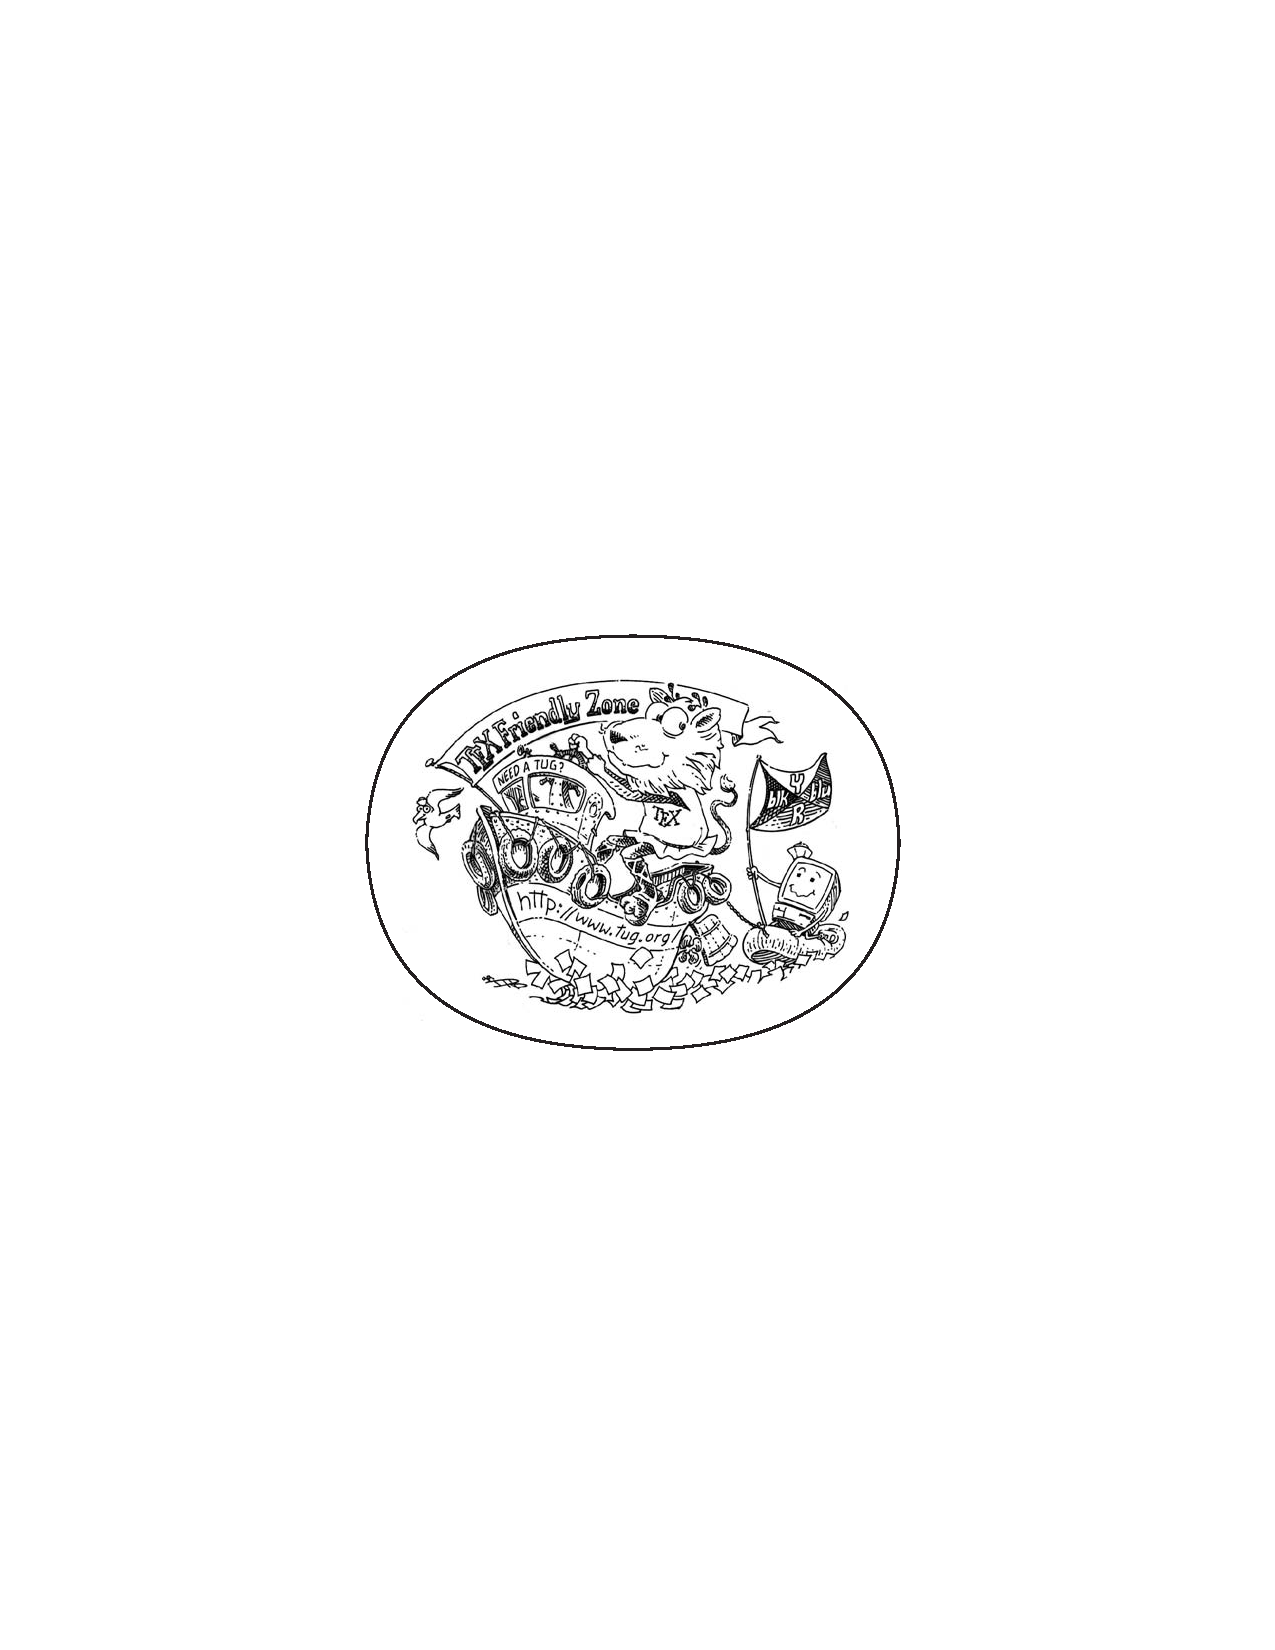
\includegraphics[width=6cm]{gfx/TFZsuperellipse_bw} \\ \medskip

        \mySubtitle \\ \medskip
        %\myDegree \\
        %\myDepartment \\
        %\myFaculty \\
        %\myUni \\ \bigskip

        \myTime\ -- \myVersion

        \vfill

    \end{center}
  \end{addmargin}
\end{titlepage}

\thispagestyle{empty}

\hfill

\vfill

\noindent\myName: \textit{\myTitle,} \mySubtitle, %\myDegree,
\textcopyright\ \myTime

%\bigskip
%
%\noindent\spacedlowsmallcaps{Supervisors}: \\
%\myProf \\
%\myOtherProf \\
%\mySupervisor
%
%\medskip
%
%\noindent\spacedlowsmallcaps{Location}: \\
%\myLocation
%
%\medskip
%
%\noindent\spacedlowsmallcaps{Time Frame}: \\
%\myTime

\cleardoublepage%*******************************************************
% Dedication
%*******************************************************
\thispagestyle{empty}
\phantomsection
\pdfbookmark[1]{Dedication}{Dedication}

\vspace*{3cm}

\begin{center}
    For Claudia and Emil \\ \smallskip
\end{center}

\cleardoublepage\include{FrontBackmatter/Foreword}
\cleardoublepage%*******************************************************
% Abstract
%*******************************************************
%\renewcommand{\abstractname}{Abstract}
\pdfbookmark[1]{Abstract}{Abstract}
% \addcontentsline{toc}{chapter}{\tocEntry{Abstract}}
\begingroup
\let\clearpage\relax
\let\cleardoublepage\relax
\let\cleardoublepage\relax

\chapter*{Abstract}
Everyday uses of audio recordings involve mixture signals: music contains a mixture of instruments; in a meeting or conference, there is a mixture of human voices.
Although human listeners find it easy to focus their attention on a particular sound source, automatically counting and separating sources remains a challenging task.
When two instruments play the same note (unison) or when many people speak concurrently (``cocktail party''), the overlap is severe, highlighting the need for new representations and powerful models to address these two tasks.
A common assumption when separating sources in the time-frequency domain (as in the case of non-negative matrix factorization) is that they are not fully overlapped.
Accurately estimating the number of sources is very important for real-world scenarios.
However, most approaches have relied on non-overlapping segments to facilitate ``counting by detection'' but with a higher amount of overlap, strategies need to shift towards directly inferring a count.
To address both problems, we used conventional signal processing techniques as well as deep neural networks (DNN).
We first address the source separation problem for unison instrument mixtures, 
thoroughly studying the distinct spectro-temporal modulations caused by vibrato. 
To exploit these modulations, we develop a method based on time warping informed by an estimate of the fundamental frequency. 
For cases where such estimates are not available, we present an unsupervised model, inspired by the way humans group time-varying sources (common fate).
This contribution comes with a novel representation that increases separability for overlapped and modulated sources on unison mixtures but also improves vocal/accompaniment separation when used as an input for a DNN model.
We approach the count estimation task by studying how humans can solve this tasks by conducting listening experiments, confirming that humans are only able to estimate up to four sources correctly.
To answer the question if machines can perform similarly, we present a DNN architecture, trained to estimate the number of concurrent speakers in a cocktail party scenario of up to ten speakers.
Our results show improvements compared to other methods, and the model even outperformed humans on the same task.
In this thesis, we affirmed the importance of modulation based signal separation. 
Our speaker count estimation model enables applications such as crowd surveillance or speaker diarization in challenging environments.
Finally, we inspected our count estimation model to glean insights on how it achieves its high performance, finding that modulations also play a crucial role in its workings.

\vfill

\begin{otherlanguage}{ngerman}
\pdfbookmark[1]{Zusammenfassung}{Zusammenfassung}
\chapter*{Zusammenfassung}

In unserem Alltag sind wir ständig von Signalmischungen umgeben: Musik  besteht aus einer Mischung von Instrumenten; in einem Meeting oder auf einer Konferenz sind wir Mischungen der menschlichen Stimme ausgesetzt.
Obwohl es für den menschlichen Zuhörer leicht ist, seine Aufmerksamkeit auf eine bestimmte Klangquelle zu fokussieren, bleibt die automatische Zählung und Trennung der Quellen eine anspruchsvolle Aufgabe.
Wenn zwei Instrumente die gleiche Note spielen (Unisono) oder wenn viele Menschen gleichzeitig sprechen (``Cocktail-Party''), ist die Überlappung groß, was die Notwendigkeit an neuen Repräsentationen und leistungsfähiger Modelle zur Bewältigung dieser beiden Aufgaben unterstreicht.
Bei der Trennung von Quellen im Zeit-Frequenzbereich (wie bei der nicht-negativen Matrixfaktorisierung) wird häufig angenommen, dass die Quellen nicht vollständig überlappt sind.
Die meisten Ansätze haben sich jedoch auf nicht überlappende Segmente konzentriert um eine Zählung durch Erkennung zu erleichtern, aber mit einer grösseren Überlappung müssen die Strategien hinzu eine direkten  Anzahl verlagert werden.
Die genaue Schätzung der Anzahl von Quellen ist für reale Szenarien sehr wichtig.
Um beide Probleme zu lösen, verwendeten wir sowohl konventionelle Signalverarbeitungstechniken als auch tiefgehendes neuronale Netze (DNN).
Wir gehen zunächst auf das Problem der Quellentrennung für unisono Instrumentenmischungen ein und untersuchen gründlich die unterschiedlichen zeitlich-spektralen Modulationen, verursacht durch Vibrato. 
Um diese Modulationen auszunutzen, entwickeln wir eine Methode, die auf dem Zeitverzerrung basiert und eine Schätzung der Grundfrequenz als zusätzliche Information nutzt.
Für Fälle, in denen diese Schätzungen nicht verfügbar sind, stellen wir ein unüberwachtes Modell vor, das inspiriert ist von der Art und Weise  wie Menschen zeitveränderliche Quellen gruppieren (Common Fate).
Dieser Beitrag enthält eine neuartige Repräsentation, die die Separierbarkeit für überlappte und modulierte Quellen in  Unisono-Mischungen erhöht, aber auch die Trennung in Gesang und Begleitung verbessert, wenn sie eingangs für ein DNN-Modell verwendet wird.
Wir bearbeiten die Aufgabe, die Anzahl von Quellen zu schätzen, indem wir zunächst untersuchen wie Menschen diese Aufgaben durch Hörversuche lösen können und bestätigen, dass Menschen nur in der Lage sind, bis zu vier Quellen korrekt in der Anzahl zu schätzen.
Um die Frage zu beantworten, ob Maschinen diese Aufgabe ähnlich gut bewältigen können, stellen wir eine DNN-Architektur vor, die erlernt hat, die Anzahl der gleichzeitigen Sprecher in einer Cocktail-Party-Umgebung von bis zu zehn Sprechern zu schätzen.
Unsere Ergebnisse zeigen Verbesserungen im Vergleich zu anderen Methoden, und das Modell übertraf sogar die Leistung des Menschen bei in der gleichen Aufgabe.
In dieser Arbeit haben wir bestätigt, wie wichtig die modulationsbasierte Signaltrennung ist. 
Unser Modell zur Schätzung der Sprecherzahl ermöglicht Anwendungen wie die Überwachung von Menschenmassen oder die beantwortung der Frage nach ``Wer spricht wann?'' in schwierigen Umgebungen.
Schließlich haben wir unser Schätzmodell für die Anzahl genau untersucht, um Erkenntnisse darüber zu gewinnen, warum es so leistungsfähig ist, und festgestellt, dass Modulationen auch hier eine entscheidende Rolle spielen.
\end{otherlanguage}

\endgroup

\vfill

\cleardoublepage%*******************************************************
% Publications
%*******************************************************
\pdfbookmark[1]{Publications}{publications}
\chapter*{Publications}
Chapters 4-8 of this thesis is mainly build upon the following publications that I published as first author during my time as a doctoral student.

\newcommand*{\boldnames}{}

\newbibmacro*{name:bold}[2]{%
  \def\do##1{\ifstrequal{#1, #2}{##1}{\bfseries\listbreak}{}}%
  \dolistloop{\boldnames}}


\xpretobibmacro{name:last}{\begingroup\usebibmacro{name:bold}{#1}{#2}}{}{}
\xpretobibmacro{name:first-last}{\begingroup\usebibmacro{name:bold}{#1}{#2}}{}{}
\xpretobibmacro{name:last-first}{\begingroup\usebibmacro{name:bold}{#1}{#2}}{}{}
\xpretobibmacro{name:delim}{\begingroup\normalfont}{}{}
\xapptobibmacro{name:last}{\endgroup}{}{}
\xapptobibmacro{name:first-last}{\endgroup}{}{}
\xapptobibmacro{name:last-first}{\endgroup}{}{}
\xapptobibmacro{name:delim}{\endgroup}{}{}

% \DeclareNameAlias{default}{last-first/first-last}

\DeclareFieldFormat{labelnumberwidth}{#1\adddot}
\newlength{\periodwidth}
\settowidth{\periodwidth}{.}

\defbibenvironment{numbered+bold}
  {\list
     {\printtext[labelnumberwidth]{%
        \printfield{prefixnumber}%
        \printfield{labelnumber}%
        }%
     }%
  {
   \setlength{\labelwidth}{\labelnumberwidth}%
   \setlength{\leftmargin}{\labelwidth}%
   \setlength{\labelsep}{\biblabelsep}%
   \addtolength{\labelsep}{1em}
   \addtolength{\leftmargin}{\labelsep}%
   \setlength{\itemsep}{\bibitemsep}%
   \setlength{\parsep}{\bibparsep}}%
   \renewcommand*{\makelabel}[1]{\hss##1}%
  }
  {\endlist}
  {\item\hskip-\periodwidth}


\newrefcontext[sorting=ynt]
\section*{Main Publications}

\begin{itemize}
  \item[\cite{stoeter19}] ~\fullcite{stoeter19}.
  \item[\cite{stoeter18}] ~\fullcite{stoeter18}.
\end{itemize}
\noindent
The publications were a result of collaboration with Soumitro Chakrabarty and Emanuël Habets. 
My contribution to this work was the initial problem formulation and the core idea to address the problem using deep neural networks. Furthermore, I designed the dataset design experimental design, and evaluation.
My college Soumitro Chakrabarty contributed to the development of the deep learning method; Emanuël Habets and Bernd Edler revised the articles.

\begin{itemize}
  \item[\cite{stoeter16}] ~\fullcite{stoeter16}.
\end{itemize}
\noindent
My contribution to this work was the experimental design, implementation and evaluation.
The original idea was developed by Antoine Liutkus, who also helped formulating the theory. Paul Magron provided code and results to compare with the HR-NMF method. Roland Badeau and Bernd Edler revised the article.

\begin{itemize}
  \item[\cite{stoeter15icassp}] ~\fullcite{stoeter15icassp}.
\end{itemize}
\noindent
My contribution in this work was the initial idea, literature overview of $F0$ estimation algorithm and the evaluation of the algorithms.
The work was done in close collaboration with my colleague Nils Werner who contributed to the efficient implementation of the $F0$ warping algorithm and the generation of appropriate warp contours to match mathematical constraints of time-warping. Bernd Edler revised this thesis.

\begin{itemize}
  \item[\cite{stoeter15acm}] ~\fullcite{stoeter15acm}.
\end{itemize}
\noindent
My contribution in this work was the initial idea which was inspired by the gap in existing $F0$ estimation datasets not providing sufficient level of annotation to derive an accurate ground truth.
The work was done together with our student, Michael Müller, who greatly helped to design and manufacture the custom experiment hardware, organize the actual recording and provide an assistance in analyzing and converting the recorded data.

\begin{itemize}
  \item[\cite{stoeter14}] ~\fullcite{stoeter14}.
\end{itemize}
\noindent
My contribution to this work was the initial idea, as well as the experimental design, and evaluation.
My college Stefan Bayer contributed important insights about the theory and implementation of time warping framework and formulated the mathematical notation therein. Bernd Edler revised the article.

\begin{itemize}
  \item[\cite{stoeter13}] ~\fullcite{stoeter13}.
\end{itemize}
\noindent
The work was based on a collaboration with Michael Schöffler and Jürgen Herre.
My contribution to this work was the initial idea, as well as the experimental prototype design, and evaluation.
My college Michael Schöffler contributed to the development of the web based evaluation software that later led to a follow-up publication~\cite{schoeffler13} which I co-authored. The article was revised by Jürgen Herre and Bernd Edler.



\section*{Additional Publications}
The following publications were not reprinted in this thesis but are nonetheless very closely related to audio based methods presented in this thesis.
\begin{refsection}[ownsideref.bib]
\nocite{*}
\printbibliography[env=numbered+bold, heading=none,resetnumbers=true, sorting=ynt]
\newrefcontext[sorting=nyt]
\end{refsection}

\section*{Open Datasets and Software}
To foster reproducible research, the following datasets and code were contributed under open licenses:
\begin{refsection}[owndata.bib]
\nocite{*}
\printbibliography[env=numbered+bold, heading=none,resetnumbers=true, sorting=ynt]
\newrefcontext[sorting=nyt]
\end{refsection}

\cleardoublepage%*******************************************************
% Acknowledgments
%*******************************************************
\pdfbookmark[1]{Acknowledgments}{acknowledgments}

\bigskip

\begingroup
\let\clearpage\relax
\let\cleardoublepage\relax
\let\cleardoublepage\relax
\chapter*{Acknowledgments}

First of all, I want to thank my supervisor Prof. Dr.-Ing. Bernd Edler for all his help and support throughout all the years. Bernd is the nicest and kindest supervisor anyone could have: his door was always open for me to have fruitful discussions and solve tricky problems together and at the same time he was giving me enough freedom to allow me to develop my own research ideas.

\bigskip

Besides my advisor, I want to thank Prof. Gaël Richard for taking the time to review my thesis.

\bigskip
I also want to thank Dr. Antoine Liutkus for inviting me to Nancy for a summer research visit that resulted in so many good ideas and a great friendship!

\bigskip

I want to thank all the amazing people in the AudioLabs, which made my work in Erlangen so enjoyable: First, I want to thank Elke, Tracy and Day-See for all the administrative help and beyond. Then, I want to thank Stefan Turowski for his great technical management in the AudioLabs. Next, I want to thank all of the colleagues at the AudioLabs (in alphabetical order): 
Alexander Adami, Stefan Bayer, Stefan Balke, Sebastian Braun, Tom Bäckström, Soumitro Chakrabarty, Youssef El Baba, Alexandra Craciun, Christian Dittmar, Sascha Disch, Jonathan Driedger, Esther Feichtner, Johannes Fischer, Yesenia Lacouture Parodi, Emanuël Habets, Jürgen Herre, Nanzhu Jiang, Patricio Lopez-Serrano, Wolfgang Mack, Goran Markovic, Vlora Arifi Müller, Meinard Müller, Thomas Prätzlich, Sebastian Rosenzweig, Konstantin Schmidt, Michael Schöffler, Armin Taghipour, Stefan Turowski, Maja Taseska, Maria Luis Valero, Elke Weiland, Christof Weiß, Nils Werner, Frank Zalkow and Julia Zalkow. Thanks to the people at Fraunhofer IIS, especially to Sascha Disch, Christopher Oates, Frederik Nagel, Christian Uhle.
And I also want to thank Thomas Zeiser from the RRZE high performance cluster for his great support.
In this vein, I want thank to all the great scientific open source tools out there that powered most of the experiments in this thesis.
\bigskip

A big thank to the students and interns I supervised and I thank them for all the great work: Berkan Ercan, Erik Johnson, Aravindh Krishnamoorty, Jeremy Hunt, Bufei Liu and Qiao Wang. 
To Karlheinz Busch from the Bamberg Symphonic Orchestra, Johannes Huber and Michael Müller for making our datasets possible. 

\bigskip

To Annika, Lisa, Florian, Chris and Chris for the great time Nuremberg and to Mathieu, Cheryl and Elias for the warm welcome in Montpellier.
I also want to thank the Faller family for their great support during the hard times of writing this thesis.

\bigskip

I deeply thank my family --- Dagmar, Heinrich and Marion --- for supporting me in every point of time in my life.

\bigskip

And last but not least, I want to thank my beloved partner and friend Claudia who gave me so much joy and hope that this journey succeeds.

\bigskip

...and to my son Emil for his beautiful smile.

\endgroup

\cleardoublepage%*******************************************************
% Table of Contents
%*******************************************************
\pagestyle{scrheadings}
%\phantomsection
\pdfbookmark[1]{\contentsname}{tableofcontents}
\setcounter{tocdepth}{1} % <-- 1 includes up to sections in the ToC
\setcounter{secnumdepth}{2} % <-- 2 numbers up to subsections
\manualmark
\markboth{\spacedlowsmallcaps{\contentsname}}{\spacedlowsmallcaps{\contentsname}}
\tableofcontents
\automark[section]{chapter}
\renewcommand{\chaptermark}[1]{\markboth{\spacedlowsmallcaps{#1}}{\spacedlowsmallcaps{#1}}}
\renewcommand{\sectionmark}[1]{\markright{\textsc{\thesection}\enspace\spacedlowsmallcaps{#1}}}
%*******************************************************
% List of Figures and of the Tables
%*******************************************************
\clearpage
% \pagestyle{empty} % Uncomment this line if your lists should not have any headlines with section name and page number
\begingroup
    \let\clearpage\relax
    \let\cleardoublepage\relax
    %*******************************************************
    % List of Figures
    %*******************************************************
    %\phantomsection
    %\addcontentsline{toc}{chapter}{\listfigurename}
    % \pdfbookmark[1]{\listfigurename}{lof}
    % \listoffigures

    % \vspace{8ex}

    %*******************************************************
    % List of Tables
    %*******************************************************
    %\phantomsection
    %\addcontentsline{toc}{chapter}{\listtablename}
    % \pdfbookmark[1]{\listtablename}{lot}
    % \listoftables

    % \vspace{8ex}
    % \newpage

    %*******************************************************
    % List of Listings
    %*******************************************************
    %\phantomsection
    %\addcontentsline{toc}{chapter}{\lstlistlistingname}
    % \pdfbookmark[1]{\lstlistlistingname}{lol}
    % \lstlistoflistings

    % \vspace{8ex}

    %*******************************************************
    % Acronyms
    %*******************************************************
    %\phantomsection
    \pdfbookmark[1]{Acronyms}{acronyms}
    \markboth{\spacedlowsmallcaps{Acronyms}}{\spacedlowsmallcaps{Acronyms}}
    \chapter*{Acronyms}
    \begin{acronym}[UMLX]
        \acro{DRY}{Don't Repeat Yourself}
        \acro{API}{Application Programming Interface}
        \acro{UML}{Unified Modeling Language}
    \end{acronym}

\endgroup

%********************************************************************
% Mainmatter
%*******************************************************
\cleardoublepage
\pagestyle{scrheadings}
\pagenumbering{arabic}
%\setcounter{page}{90}
% use \cleardoublepage here to avoid problems with pdfbookmark
\cleardoublepage
% \include{Chapters/DAFx14_StoeterEdler}
\cleardoublepage
\ctparttext{You can put some informational part preamble text here.
Illo principalmente su nos. Non message \emph{occidental} angloromanic
da. Debitas effortio simplbificate sia se, auxiliar summarios da que,
se avantiate publicationes via. Pan in terra summarios, capital
interlingua se que. Al via multo esser specimen, campo responder que
da. Le usate medical addresses pro, europa origine sanctificate nos se.}

%************************************************
\chapter{Introduction}\label{ch:introduction}
%************************************************
This bundle for \LaTeX\ has two goals:
\begin{enumerate}
    \item Provide students with an easy-to-use template for their
    Master's
    or PhD thesis. (Though it might also be used by other types of
    authors
    for reports, books, etc.)
    \item Provide a classic, high-quality typographic style that is
    inspired by \citeauthor{bringhurst:2002}'s ``\emph{The Elements of
    Typographic Style}'' \citep{bringhurst:2002}.
    \marginpar{\myTitle \myVersion}
\end{enumerate}
The bundle is configured to run with a \emph{full}
MiK\TeX\ or \TeX Live\footnote{See the file \texttt{LISTOFFILES} for
needed packages. Furthermore, \texttt{classicthesis}
works with most other distributions and, thus, with most systems
\LaTeX\ is available for.}
installation right away and, therefore, it uses only freely available
fonts. (Minion fans can easily adjust the style to their needs.)

People interested only in the nice style and not the whole bundle can
now use the style stand-alone via the file \texttt{classicthesis.sty}.
This works now also with ``plain'' \LaTeX.

As of version 3.0, \texttt{classicthesis} can also be easily used with
\mLyX\footnote{\url{http://www.lyx.org}} thanks to Nicholas Mariette
and Ivo Pletikosić. The \mLyX\ version of this manual will contain
more information on the details.

This should enable anyone with a basic knowledge of \LaTeXe\ or \mLyX\ to
produce beautiful documents without too much effort. In the end, this
is my overall goal: more beautiful documents, especially theses, as I
am tired of seeing so many ugly ones.

The whole template and the used style is released under the
\acsfont{GNU} General Public License.

If you like the style then I would appreciate a postcard:
\begin{center}
    André Miede \\
    Detmolder Straße 32 \\
    31737 Rinteln \\
    Germany
\end{center}
The postcards I received so far are available at:
\begin{center}
    \url{http://postcards.miede.de}
\end{center}
\marginpar{A well-balanced line width improves the legibility of
the text. That's what typography is all about, right?}
So far, many theses, some books, and several other publications have
been typeset successfully with it. If you are interested in some
typographic details behind it, enjoy Robert Bringhurst's wonderful book.
% \citep{bringhurst:2002}.

\paragraph{Important Note:} Some things of this style might look
unusual at first glance, many people feel so in the beginning.
However, all things are intentionally designed to be as they are,
especially these:
\begin{itemize}
    \item No bold fonts are used. Italics or spaced small caps do the
    job quite well.
    \item The size of the text body is intentionally shaped like it
    is. It supports both legibility and allows a reasonable amount of
    information to be on a page. And, no: the lines are not too short.
    \item The tables intentionally do not use vertical or double
    rules. See the documentation for the \texttt{booktabs} package for
    a nice discussion of this topic.\footnote{To be found online at
    \url{http://mirror.ctan.org/macros/latex/contrib/booktabs/}.}
    \item And last but not least, to provide the reader with a way
    easier access to page numbers in the table of contents, the page
    numbers are right behind the titles. Yes, they are \emph{not}
    neatly aligned at the right side and they are \emph{not} connected
    with dots that help the eye to bridge a distance that is not
    necessary. If you are still not convinced: is your reader
    interested in the page number or does she want to sum the numbers
    up?
\end{itemize}
Therefore, please do not break the beauty of the style by changing
these things unless you really know what you are doing! Please.

\paragraph{Yet Another Important Note:} Since \texttt{classicthesis}'
first release in 2006, many things have changed in the \LaTeX\ world.
Trying to keep up-to-date, \texttt{classicthesis} grew and evolved
into many directions, trying to stay (some kind of) stable and be
compatible with its port to \mLyX. However, there are still many
remains from older times in the code, many dirty workarounds here and
there, and several other things I am absolutely not proud of (for
example my unwise combination of \acsfont{KOMA} and
\texttt{titlesec} etc.).
\graffito{An outlook into the future of \texttt{classicthesis}.}

Currently, I am looking into how to completely re-design and
re-implement \texttt{classicthesis} making it easier to maintain and
to use. As a general idea, \texttt{classicthesis.sty} should be
developed and distributed separately from the template bundle itself.
Excellent spin-offs such as \texttt{arsclassica} could also be
integrated (with permission by their authors) as format configurations.
Also, current trends of \texttt{microtype}, \texttt{fontspec}, etc.
should be included as well. As I am not really into deep
\LaTeX\ programming,
I will reach out to the \LaTeX\ community for their expertise and help.


\section{Motivation}
A very important factor for successful thesis writing is the
organization of the material. This template suggests a structure as
the following:
\begin{itemize}
    \marginpar{You can use these margins for summaries of the text
    body\dots}
    \item\texttt{Chapters/} is where all the ``real'' content goes in
    separate files such as \texttt{Chapter01.tex} etc.
    % \item\texttt{Examples/} is where you store all listings and other
    % examples you want to use for your text.
    \item\texttt{FrontBackMatter/} is where all the stuff goes that
    surrounds the ``real'' content, such as the acknowledgments,
    dedication, etc.
    \item\texttt{gfx/} is where you put all the graphics you use in
    the thesis. Maybe they should be organized into subfolders
    depending on the chapter they are used in, if you have a lot of
    graphics.
    \item\texttt{Bibliography.bib}: the Bib\TeX\ database to organize
    all the references you might want to cite.
    \item\texttt{classicthesis.sty}: the style definition to get this
    awesome look and feel. Does not only work with this thesis template
    but also on its own (see folder \texttt{Examples}). Bonus: works
    with both \LaTeX\ and \textsc{pdf}\LaTeX\dots and \mLyX.
    % \item\texttt{ClassicThesis.tcp} a \TeX nicCenter project file.
    Great tool and it's free!
    \item\texttt{ClassicThesis.tex}: the main file of your thesis
    where all gets bundled together.
    \item\texttt{classicthesis-config.tex}: a central place to load all
    nifty packages that are used. % In there, you can also activate
    % backrefs in order to have information in the bibliography about
    % where a source was cited in the text (\ie, the page number).

    \emph{Make your changes and adjustments here.} This means that you
    specify here the options you want to load \texttt{classicthesis.sty}
    with. You also adjust the title of your thesis, your name, and all
    similar information here. Refer to \autoref{sec:custom} for more
    information.

    This had to change as of version 3.0 in order to enable an easy
    transition from the ``basic'' style to \mLyX.
\end{itemize}
In total, this should get you started in no time.


\clearpage
\section{Contributions}\label{sec:options}
There are a couple of options for \texttt{classicthesis.sty} that
allow for a bit of freedom concerning the layout:
\marginpar{\dots or your supervisor might use the margins for some
    comments of her own while reading.}
\begin{itemize}
    \item General:
        \begin{itemize}
            \item\texttt{drafting}: prints the date and time at the bottom of
            each page, so you always know which version you are dealing with.
            Might come in handy not to give your Prof. that old draft.
        \end{itemize}

    \item Parts and Chapters:
        \begin{itemize}
            \item\texttt{parts}: if you use Part divisions for your document,
            you should choose this option. (Cannot be used together with
            \texttt{nochapters}.)

            \item\texttt{linedheaders}: changes the look of the chapter
            headings a bit by adding a horizontal line above the chapter
            title. The chapter number will also be moved to the top of the
            page, above the chapter title.
        \end{itemize}

    \item Typography:
        \begin{itemize}
            \item\texttt{palatino}: Hermann Zapf's classic font is the free standard font for this style. Robert Bringhurst's book uses Adobe's commercial font Minion Pro. However, there are other free alternatives also available. Deactivate this option for loading such alternatives and see \texttt{classicthesis-config.tex} for some suggestions.

            \item\texttt{eulerchapternumbers}: use figures from Hermann Zapf's
            Euler math font for the chapter numbers. By default, old style
            figures from the Palatino font are used.

            \item\texttt{beramono}: loads Bera Mono as typewriter font.
            (Default setting is using the standard CM typewriter font.)

            \item\texttt{eulermath}: loads the awesome Euler fonts for math.
            Pala\-tino is used as default font.
        \end{itemize}

    \marginpar{Options are enabled via \texttt{option=true}}

    \item Table of Contents:
        \begin{itemize}
            \item\texttt{tocaligned}: aligns the whole table of contents on
            the left side. Some people like that, some don't.

            \item\texttt{dottedtoc}: sets pagenumbers flushed right in the
            table of contents.

            \item\texttt{manychapters}: if you need more than nine chapters for
            your document, you might not be happy with the spacing between the
            chapter number and the chapter title in the Table of Contents.
            This option allows for additional space in this context.
            However, it does not look as ``perfect'' if you use
            \verb|\parts| for structuring your document.
        \end{itemize}

    \item Floats:
        \begin{itemize}
            % \item\texttt{listings}: loads the \texttt{listings} package (if not already done) and configures the List of Listings accordingly.

            \item\texttt{floatperchapter}: activates numbering per chapter for
            all floats such as figures, tables, and listings (if used).
        \end{itemize}

\end{itemize}

Furthermore, pre-defined margins for different paper sizes are available, \eg, \texttt{a4paper}, \texttt{a5paper}, \texttt{b5paper}, and \texttt{letterpaper}. These are based on your chosen option of \verb|\documentclass|.

The best way to figure these options out is to try the different
possibilities and see what you and your supervisor like best.

In order to make things easier, \texttt{classicthesis-config.tex}
contains some useful commands that might help you.


\section{Thesis Outline}\label{sec:custom}
%(As of v3.0, the Classic Thesis Style for \LaTeX{} and \mLyX{} share
%the same two \texttt{.sty} files.)
This section will show you some hints how to adapt
\texttt{classicthesis} to your needs.

The file \texttt{classicthesis.sty}
contains the core functionality of the style and in most cases will
be left intact, whereas the file \texttt{classic\-thesis-config.tex}
is used for some common user customizations.

The first customization you are about to make is to alter the document
title, author name, and other thesis details. In order to do this, replace
the data in the following lines of \texttt{classicthesis-config.tex:}%
\marginpar{Modifications in \texttt{classic\-thesis-config.tex}%
}

\begin{lstlisting}
    % **************************************************
    % 2. Personal data and user ad-hoc commands
    % **************************************************
    \newcommand{\myTitle}{A Classic Thesis Style\xspace}
    \newcommand{\mySubtitle}{An Homage to...\xspace}
\end{lstlisting}

Further customization can be made in \texttt{classicthesis-config.tex}
by choosing the options to \texttt{classicthesis.sty}
(see~\autoref{sec:options}) in a line that looks like this:

\begin{lstlisting}
\PassOptionsToPackage{
  drafting=true,    % print version information on the bottom of the pages
  tocaligned=false, % the left column of the toc will be aligned (no indentation)
  dottedtoc=false,  % page numbers in ToC flushed right
  parts=true,       % use part division
  eulerchapternumbers=true, % use AMS Euler for chapter font (otherwise Palatino)
  linedheaders=false,       % chaper headers will have line above and beneath
  floatperchapter=true,     % numbering per chapter for all floats (i.e., Figure 1.1)
  eulermath=false,  % use awesome Euler fonts for mathematical formulae (only with pdfLaTeX)
  beramono=true,    % toggle a nice monospaced font (w/ bold)
  % palatino=false, % deactivate standard font for loading another one, see the last section at the end of this file for suggestions
}{classicthesis}
\end{lstlisting}

Many other customizations in \texttt{classicthesis-config.tex} are
possible, but you should be careful making changes there, since some
changes could cause errors.

% Finally, changes can be made in the file \texttt{classicthesis.sty},%
% \marginpar{Modifications in \texttt{classicthesis.sty}%
% } although this is mostly not designed for user customization. The
% main change that might be made here is the text-block size, for example,
% to get longer lines of text.


This section will list some information about problems using
\texttt{classic\-thesis} in general or using it with other packages.

Beta versions of \texttt{classicthesis} can be found at Bitbucket:
\begin{center}
    \url{https://bitbucket.org/amiede/classicthesis/}
\end{center}
There, you can also post serious bugs and problems you encounter.


So far, this is a quite stable version that served a couple of people
well during their thesis time. However, some things are still not as
they should be. Proper documentation in the standard format is still
missing. In the long run, the style should probably be published
separately, with the template bundle being only an application of the
style. Alas, there is no time for that at the moment\dots it could be
a nice task for a small group of \LaTeX nicians.

Please do not send me email with questions concerning \LaTeX\ or the
template, as I do not have time for an answer. But if you have
comments, suggestions, or improvements for the style or the template
in general, do not hesitate to write them on that postcard of yours.

The layout of \texttt{classicthesis.sty} can be easily used without the
framework of this template. A few examples where it was used to typeset
an article, a book or a curriculum vitae can be found in the folder
\texttt{Examples}. The examples have been tested with
\texttt{latex} and \texttt{pdflatex} and are easy to compile. To
encourage you even more, PDFs built from the sources can be found in the
same folder.


\paragraph{GNU General Public License:} This program is free software;
you can redistribute it and/or modify
it under the terms of the \acsfont{GNU} General Public License as
published by
the Free Software Foundation; either version 2 of the License, or
(at your option) any later version.

This program is distributed in the hope that it will be useful,
but \emph{without any warranty}; without even the implied warranty of
\emph{merchant\-ability} or \emph{fitness for a particular purpose}.
See the
\acsfont{GNU} General Public License for more details.

You should have received a copy of the \acsfont{GNU} General
Public License
along with this program; see the file \texttt{COPYING}.  If not,
write to
the Free Software Foundation, Inc., 59 Temple Place - Suite 330,
Boston, MA 02111-1307, USA.

\paragraph{classichthesis Authors' note:} There have been some discussions about the GPL's implications on using \texttt{classicthesis} for theses etc. Details can be found here:
\begin{center}
  \url{https://bitbucket.org/amiede/classicthesis/issues/123/}
\end{center}

We chose (and currently stick with) the GPL because we would not like to compete with proprietary modified versions of our own work. However, the whole template is free as free beer and free speech. We will not demand the sources for theses, books, CVs, etc. that were created using \texttt{classicthesis}.

Postcards are still highly appreciated.





%*****************************************
%*****************************************
%*****************************************
%*****************************************
%*****************************************


\part{fundamentals}

\section{Fundamentals of Overlapped Signals}
\kant[1-12]
\section{Signal Representations}
\kant[1-8]
\subsection{Time domain signal representation}
\kant[1-6]
\subsection{Time-Frequency Representations}
\kant[1-6]

\section{Specificies of Real World Overlapped Audio Signals (Music, Speech)}
\kant[1-6]

\subsection{Harmonicity and Pitch}
\kant[1-6]

\subsection{Temporal aspects}
\kant[1-6]

\subsection{Modulational Aspects}
\kant[1-6]

\subsection{Acoustic aspects}
\kant[1-6]

\subsection{Subjective aspects}
\kant[1-6]


\section{Scenarios and Applications}
\kant[1-6]

\subsection{Cocktail Party Environment}
\kant[1-4]

\subsection{Unison Mixtures}
\kant[1-4]

\subsection{Professional Produced Music}
\kant[1-4]


\part{Source Separation}\label{pt:showcase}

\chapter{Separation of Unison Sources}



% \section{Introduction}
% \label{sec:intro}

% Intro DAFx

Audio source separation is a very active research field with a large number of contributions. Applications are dependent on the context of the scenario, ranging from enhancements of speech signals to musically motivated analysis tasks.

% TODO Listing more application

The separation of sound sources from a single channel mixture is considered as an under-determined case which does not have a single solution. Knowing the way in which source signals are mixed together is crucial to the quality of separation systems. In the context of speech separation even unsupervised methods can lead to good results. This is due to the fact that mixtures of speech signals (like in a cocktail party environment) show a high degree of statistical independence. Mixtures of musical instruments, however, are highly correlated which is a desired aim of musical performances in general.

The Signal Separation Evaluation Campaign (SiSEC) is a solid indicator of the progress in research within the field of source separation \cite{vincent2012signal}. The results from 2013 \cite{sisec2013} show that for professionally produced music it is still difficult to achieve a high quality separation.
One reason is due to the fact that the wide use of non-linear post-processing techniques (e.g. dynamic compression or effects like reverb) break assumptions that often are required to enable good performance of source separation algorithms. Another reason is that non-stationary effects like vibrato introduce additional problems \cite{nakano2010nonnegative}.

In most scenarios for source separation of instrument signals it is common to assume that the spectral harmonics do only partially overlap. This enables algorithms like non-negative matrix factorization (NMF) to approximate the mixture from a lower-rank decomposition in an unsupervised way. Such systems are described in \cite{smaragdis2003non} and \cite{virtanen2007monaural}. Additionally the popularity of the class of NMF algorithms can be explained by the intuitive way in which they work on time-frequency representations of the mixture signal.

In the context of musical instrument source separation, many researchers have focused on including prior information about the sources in their algorithms \cite{ozerov2012general}. The availability and detail of such a-priori information varies. Often systems learn spectral as well as temporal cues from training data or parts of the mixture where only one instrument is active. One example of such informed source separation systems is described by Ewert and M\"uller \cite{ewert2012using}. It incorporates the pitch and onset information encoded in a MIDI file to improve the separation result.

Even the number of sources is a simple but very important information for source separation algorithms. One of the main drawbacks of many source separation systems is that they rely on this information. In some scenarios, like popular western music, the sources to separate are grouped into Melody + Bass + Drums and a residual signal. Constraining the system to such a scenario allows the results to be evaluated even if the set of sources being separated is incomplete. Constrained systems like these are also sufficient for real-world applications such as the eminent karaoke scenario. Limiting the number of desired sources helps not only to improve the performance of the algorithms but is also related to the fact that the number of sources humans can perceive is limited, too. Although a threshold has not been systematically addressed so far, a variety of experiments have been carried out. David Huron found \cite{huron89} that the number of voices humans can correctly identify is up to three. When St\"oter and Schoeffler et. al. \cite{stoter2013human, schoeffler2013experiment} asked participants to identify the number of instruments in a piece of music, the participants were only able to identify up to three, similar to Huron's voice experiments. There is very little chance that listeners are able to detect the presence of more than three sources. However in trials with fewer than three instruments, listeners tended to be very sensitive: One of the stimuli in the \cite{stoter2013human, schoeffler2013experiment} experiments with 1168 participants consisted of a mixture of Violin and Flute played in unison. The results showed that $76\%$ of the participants correctly identified two instruments. Only $18\%$ of the participants underestimated by one instrument, $6\%$ overestimated by one instrument.

Since humans are able to reliably detect even instruments played in unison,  this is a good motivation to expect the same from an algorithm. In this paper we want to address this scenario which has not been brought up so far. We believe creating and evaluating new algorithms for separating sources playing in unison will improve source separation systems in general.

The remainder of this paper is organized as follows: Section~\ref{sec:scenario} describes the challenges of a unison source separation scenario. We propose techniques based on the modulation characteristics of the signal to address the separation scenario in Section~\ref{sub:am} and Section~\ref{sub:frequency_modulation}. In Section~\ref{sec:experiment} we introduce a data set for the unison scenario. Further we present and discuss the results from our study and a comparison between the algorithms in Section~\ref{sec:results}. Conclusions are then presented in Section~\ref{sec:conclusions}.


% Intro commonfate

Sound source separation continues to be a very active field of research~\cite{vincentSSoverview2014} with a variety of applications. Many recent contributions are based on the popular non-negative matrix factorization (NMF). The way NMF factorizes a spectrogram matrix into frequency and activation templates makes it possible to easily design algorithms in an intuitive way. At the same time, it provides a rank reduction, needed to decompose mixtures into their source components.
In the past, many NMF-based source separation methods have been developed~\cite{smaragdis2003nmf, NMFD-Smaragdis04, virtanen2007monaural}. Expanding the NMF to tensors allows to incorporate more complex models, useful in many applications like multi-channel separation. Extensions to NMF such as shift-invariance or convolutions were carried over to non-negative tensor (NTF) based algorithms~\cite{fitzgerald2005non, fitzgerald2008extended, Fitzgerald06soundsource, fevotte_cmmr10, Ozerov2011}. These approaches, relying on decomposing mixtures of musical instruments, work well when certain assumptions hold to be true.
One is that spectral harmonics only partially overlap. However, when two sources share the same fundamental frequency, almost all partials do overlap, making it difficult for NMF-based algorithms to learn unique templates. Another assumption is that all spectral and temporal templates semantically correspond to musical notes, forming a dictionary of musically meaningful atoms.
This does not hold for instruments with time-varying fluctuations. These effects can typically be found in musical instruments like strings and brass, when played with vibrato. In a setting where two musical instruments with vibrato play in unison, both assumptions could break, which makes it a challenging scenario~\cite{stoeter2014}.
When processing such mixtures with a representation based on a standard NMF and the magnitude spectrogram, it is hard to model the sources with only a few spectral templates. Instead of increasing the number of templates per source, Hennequin proposes~\cite{hennequin2011nmf} frequency-dependent activation matrices by using a source/filter-based model.
Since the vibrato does not only cause frequency modulation (FM) but also amplitude modulation (AM), so-called modulation spectra can be used to identify the modulation pattern. This is often calculated by taking the Fourier transform of a magnitude spectrum. Thus, the \emph{modulation spectrogram} has already gathered much attention in speech recognition~\cite{greenberg1997modulation,kingsbury1998ASRmodulation} and  classification~\cite{kinnunen2008modulation,markaki2009usingmodulation}.
Barker and Virtanen~\cite{barker2013modulation} were the first to propose a modulation tensor representation for single channel source separation. This allows to elegantly apply factorization on the tensor by using the well known PARAFAC/CANDECOMP (CP) decomposition.

In this work we introduce a novel tensor signal representation which additionally exploits similarities in the frequency direction. We can therefore make use of dependencies between modulations of neighbouring bins. This is similar to the recently proposed High-Resolution Nonnegative Matrix Factorization
model that accounts for dependencies in the time-frequency plane (HR-NMF
~\cite{badeau2011hrnmf}). In short, HR-NMF models each complex entry of a time-frequency transform of an audio signal as a linear combination of its neighbours, enabling the modelling of damped sinusoids, along with an independent
innovation. This model was generalized to multichannel mixtures in~\cite{badeau2013multichannel_hrnmf,badeau2014hrnmfTASLP}
and was shown to provide considerably better oracle performance for source separation than alternative models in~\cite{magron2015hrnmfbenchmark}.
Indeed, even though some variational approximations were introduced
in~\cite{badeau2013variational_hrnmf} to strongly reduce their complexity,
those algorithms are often demanding for practical applications.
In this paper, we propose to relax some assumptions of HR-NMF in the interest of simplifying the estimation procedure. The core idea is to divide the complex spectrogram into modulation patches in order to group common modulation in time and frequency direction. We call this the \emph{Common Fate Model} (CFM), borrowing from the Gestalt theory, which describes how human perception merges objects that move together over time. Bregman~\cite{bregman1994auditory} described the Common Fate theory for auditory scene analysis as the ability to group sound objects based on their common motion over time, as occurs with frequency modulations of harmonic partials. As outlined by Bregman, the human ability to detect and group sound sources by small differences in FM and AM is outstanding. Also, it turns out that humans are especially sensitive to modulation frequencies around 5~Hz, which is the typical vibrato frequency that many musicians produce naturally.

\section{Unison Source Separation Scenario}
\label{sec:scenario}

Up to date there are very few proposed source separation methods which perform good on a variety of input signals without making general assumptions or constraints. Most of the current state-of-the-art algorithms address specific scenarios like voice or melody extraction, or harmonic percussive separation. Additionally assumptions about the mixture itself are important, too. In this paper we consider the linear single channel case:
\begin{equation}
  x(n) = \sum_{s = 1}^{N} x_s(n).
\end{equation}
Describing a source separation scenario includes the number of sources $N$ and the number of desired sources $D$ which is normally smaller than $N$ when the desired sources contain groups of sources like instrument classes (strings, woodwinds, etc.).

We propose a scenario where instruments play in unison. This means that they share the same fundamental frequency (regardless of the octave) so that the sources can overlap both in time and frequency. In fact unison\footnote{greek: with \emph{one voice}} mixtures are meant to be as much overlapped as possible, hence they are very difficult to separate. However, due to masking effects, a relatively good subjective quality for the separated sources can be obtained, even if the other sources are not perfectly suppressed.
As far as we know, there is no contribution to the source separation scene that focuses on mixtures of such unison sources. \\

The decomposition of sources with overlapping partials are covered in several other publications like \cite{nakano2010nonnegative} and \cite{smaragdis2008sparse} which are based on non-negative matrix factorization. Lin et. al. \cite{lintimbre} address the problem by defining invariant timbre based features. We propose to address the problem from a different perspective and focus on analyzing the non-stationarities of the source signals. For most musical instruments, the non-stationary features are intentionally created, for instance with vibrato or tremolo effects, which make them valuable to track. These non-stationarities can be modeled or learned from the signals themselves. \\

In this work we assume that we can separate overlapping partials of the sources based on differences in amplitude and/or frequency modulation, resulting in the following model for a signal with $P$ commonly modulated partials
\begin{equation}
  \begin{array}{l}
   x(n) = \displaystyle \sum_{p=1}^{P} \Big[\big(1 + a(n)\big) \\
   \hspace{3.5em}\displaystyle \cdot\sin \Big(2\pi f_{p,0}\big(n + \frac{1}{f_{1,0}} \sum_{m=m_0}^{n}{f(m)} \big) + \phi_{p,0} \Big)\Big] ,
  \end{array}
\end{equation}
where effectively the amplitude modulation is $a(n)$ and the frequency modulation of the first partial is $f(n)$.

\begin{figure}[H]
    \centering
    \tiny
    \subfloat[Input]{
       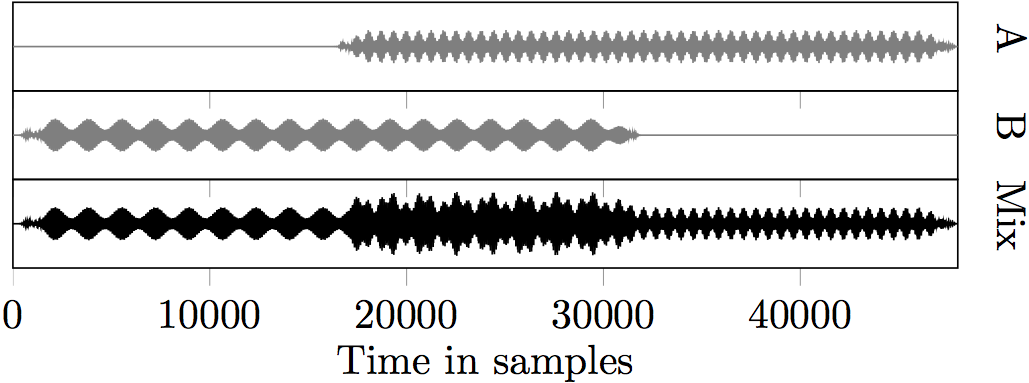
\includegraphics[width=0.92\columnwidth]{Chapters/dafx/figures/Timepdf-crop.png}	   		  \hspace{-7mm}
    }\hfill
    \subfloat[Spectrogram]{
       % This file was created by matlab2tikz% This file was created by matlab2tikz v0.4.7 (commit 3442858e5a642c135c5e9dab6a960bee5b9c6f8d) running on MATLAB 8.2.
% Copyright (c) 2008--2014, Nico Schlmer <nico.schloemer@gmail.com>
% All rights reserved.
% Minimal pgfplots version: 1.3
%
% The latest updates can be retrieved from
%   http://www.mathworks.com/matlabcentral/fileexchange/22022-matlab2tikz
% where you can also make suggestions and rate matlab2tikz.
%
\begin{tikzpicture}[font=\small]

\begin{axis}[%
width=0.15\columnwidth,
height=3.5cm,
axis on top,
xminorgrids=true,
minor xtick={1.5,2.5},
scale only axis,
xtick={1,2},
xmin=0.5,
xmax=2.5,
ymin=0.5,
ymax=137.5,
name=plot2,
xlabel=Gain Components,
ylabel=Modulation Frequency Bins,
every axis y label/.style={at={(current axis.north east)},below=18mm,xshift=8mm},
y label style={rotate=-90},
]
\addplot [forget plot] graphics [xmin=0.5,xmax=2.5,ymin=0.5,ymax=137.5] {Chapters/05_Separation_Known/figures/AMPlots/GAS-1_scaled.png};
\end{axis}

\begin{axis}[%
width=0.15\columnwidth,
height=3.5cm,
xminorgrids=true,
minor xtick={1.5,2.5},
axis on top,
scale only axis,
xtick={1,2},
xmin=0.5,
xmax=2.5,
ymin=0.5,
ymax=145.5,
xlabel=Basis Components,
ylabel=Frequency Bins,
every axis y label/.style={at={(current axis.north east)},below=18mm,xshift=8mm},
y label style={rotate=-90},
at=(plot2.left of south west),
anchor=right of south east
]
\addplot [forget plot] graphics [xmin=0.5,xmax=2.5,ymin=0.5,ymax=145.5] {Chapters/05_Separation_Known/figures/AMPlots/GAS-2_scaled.png};
\end{axis}

\begin{axis}[%
width=0.15\columnwidth,
height=3.5cm,
xminorgrids=true,
minor xtick={1.5,2.5},
axis on top,
scale only axis,
xtick={1,2},
xmin=0.5,
xmax=2.5,
ymin=0.5,
ymax=81.5,
xlabel=Activation Components,
ylabel=Frames,
every axis y label/.style={at={(current axis.north east)},below=18mm,xshift=8mm},
y label style={rotate=-90},
at=(plot2.right of south east),
anchor=left of south west
]
\addplot [forget plot] graphics [xmin=0.5,xmax=2.5,ymin=0.5,ymax=81.5] {Chapters/05_Separation_Known/figures/AMPlots/GAS-3_scaled.png};
\end{axis}
\end{tikzpicture}%
 v0.4.7 (commit 3442858e5a642c135c5e9dab6a960bee5b9c6f8d) running on MATLAB 8.2.
% Copyright (c) 2008--2014, Nico Schlmer <nico.schloemer@gmail.com>
% All rights reserved.
% Minimal pgfplots version: 1.3
%
% The latest updates can be retrieved from
%   http://www.mathworks.com/matlabcentral/fileexchange/22022-matlab2tikz
% where you can also make suggestions and rate matlab2tikz.
%
\begin{tikzpicture}[font=\small]

\begin{axis}[%
    /pgf/number format/.cd,
           use comma,
           1000 sep={},
width=0.35\columnwidth,
height=3.5cm,
axis on top,
scale only axis,
xmin=0.5,
xmax=1497.5,
ymin=0.5,
ymax=145.5,
xlabel=Frames,
ylabel=Frequency Bins,
every axis y label/.style={at={(current axis.north east)},below=18mm,xshift=4mm},
y label style={rotate=-90},
]
\addplot [forget plot] graphics [xmin=0.5,xmax=1497.5,ymin=0.5,ymax=145.5] {Chapters/dafx/figures/AMPlots/STFT-1_scaled.png};
\end{axis}
\end{tikzpicture}%
%
    }%
    \subfloat[Tensor Slice]{
       % This file was created by matlab2tikz v0.4.7 (commit 3442858e5a642c135c5e9dab6a960bee5b9c6f8d) running on MATLAB 8.2.
% Copyright (c) 2008--2014, Nico Schlmer <nico.schloemer@gmail.com>
% All rights reserved.
% Minimal pgfplots version: 1.3
%
% The latest updates can be retrieved from
%   http://www.mathworks.com/matlabcentral/fileexchange/22022-matlab2tikz
% where you can also make suggestions and rate matlab2tikz.
%
\begin{tikzpicture}[font=\small]

\begin{axis}[%
width=0.35\columnwidth,
height=3.5cm,
axis on top,
scale only axis,
xmin=0.5,
xmax=81.5,
ymin=0.5,
ymax=137.5,
xlabel=Frames,
ylabel=Modulation Frequency Bins,
every axis y label/.style={at={(current axis.north east)},below=18mm,xshift=4mm},
y label style={rotate=-90},
]
\addplot [forget plot] graphics [xmin=0.5,xmax=81.5,ymin=0.5,ymax=137.5] {Chapters/dafx/figures/AMPlots/Tmod-1_scaled.png};
\end{axis}
\end{tikzpicture}%
%
    }\hfill

    \subfloat[NMF]{
     	% This file was created by matlab2tikz v0.4.7 (commit 3442858e5a642c135c5e9dab6a960bee5b9c6f8d) running on MATLAB 8.2.
% Copyright (c) 2008--2014, Nico Schlmer <nico.schloemer@gmail.com>
% All rights reserved.
% Minimal pgfplots version: 1.3
%
% The latest updates can be retrieved from
%   http://www.mathworks.com/matlabcentral/fileexchange/22022-matlab2tikz
% where you can also make suggestions and rate matlab2tikz.
%
\begin{tikzpicture}[font=\small]

\begin{axis}[%
/pgf/number format/.cd, use comma, 1000 sep={},
width=0.225\columnwidth,
height=3.5cm,
axis on top,
scale only axis,
xtick={1,2},
xminorgrids=true,
minor xtick={1.5},
xmin=0.5,
xmax=2.5,
ymin=0.5,
ymax=145.5,
name=plot1,
xlabel=Basis Components,
ylabel=Frequency Bins,
every axis y label/.style={at={(current axis.north east)},below=18mm,xshift=4mm},
y label style={rotate=-90},
]
\addplot [forget plot] graphics [xmin=0.5,xmax=2.5,ymin=0.5,ymax=145.5] {Chapters/dafx/figures/AMPlots/WH-1_scaled.png};
\end{axis}

\begin{axis}[%
/pgf/number format/.cd, use comma, 1000 sep={},
width=0.225\columnwidth,
height=3.5cm,
axis on top,
scale only axis,
xminorgrids=true,
minor xtick={1.5},
xtick={1,2},
xmin=0.5,
xmax=2.5,
ymin=0.5,
ymax=1497.5,
xlabel=Activation Components,
ylabel=Frames,
every axis y label/.style={at={(current axis.north east)},below=18mm,xshift=4mm},
y label style={rotate=-90},
at=(plot1.right of south east),
anchor=left of south west
]
\addplot [forget plot] graphics [xmin=0.5,xmax=2.5,ymin=0.5,ymax=1497.5] {Chapters/dafx/figures/AMPlots/WH-2_scaled.png};
\end{axis}
\end{tikzpicture}%
%
    }\hfill
    \subfloat[Non-Negative Tensor Factorization]{
       % This file was created by matlab2tikz v0.4.7 (commit 3442858e5a642c135c5e9dab6a960bee5b9c6f8d) running on MATLAB 8.2.
% Copyright (c) 2008--2014, Nico Schlmer <nico.schloemer@gmail.com>
% All rights reserved.
% Minimal pgfplots version: 1.3
%
% The latest updates can be retrieved from
%   http://www.mathworks.com/matlabcentral/fileexchange/22022-matlab2tikz
% where you can also make suggestions and rate matlab2tikz.
%
\begin{tikzpicture}[font=\small]

\begin{axis}[%
width=0.225\columnwidth,
height=3.5cm,
axis on top,
xminorgrids=true,
minor xtick={1.5,2.5},
scale only axis,
xtick={1,2},
xmin=0.5,
xmax=2.5,
ymin=0.5,
ymax=137.5,
name=plot2,
xlabel=Gain Components,
ylabel=Modulation Frequency Bins,
every axis y label/.style={at={(current axis.north east)},below=18mm,xshift=4mm},
y label style={rotate=-90},
]
\addplot [forget plot] graphics [xmin=0.5,xmax=2.5,ymin=0.5,ymax=137.5] {Chapters/dafx/figures/AMPlots/GAS-1_scaled.png};
\end{axis}

\begin{axis}[%
width=0.225\columnwidth,
height=3.5cm,
xminorgrids=true,
minor xtick={1.5,2.5},
axis on top,
scale only axis,
xtick={1,2},
xmin=0.5,
xmax=2.5,
ymin=0.5,
ymax=145.5,
xlabel=Basis Components,
ylabel=Frequency Bins,
every axis y label/.style={at={(current axis.north east)},below=18mm,xshift=4mm},
y label style={rotate=-90},
at=(plot2.left of south west),
anchor=right of south east
]
\addplot [forget plot] graphics [xmin=0.5,xmax=2.5,ymin=0.5,ymax=145.5] {Chapters/dafx/figures/AMPlots/GAS-2_scaled.png};
\end{axis}

\begin{axis}[%
width=0.225\columnwidth,
height=3.5cm,
xminorgrids=true,
minor xtick={1.5,2.5},
axis on top,
scale only axis,
xtick={1,2},
xmin=0.5,
xmax=2.5,
ymin=0.5,
ymax=81.5,
xlabel=Activation Components,
ylabel=Frames,
every axis y label/.style={at={(current axis.north east)},below=18mm,xshift=4mm},
y label style={rotate=-90},
at=(plot2.right of south east),
anchor=left of south west
]
\addplot [forget plot] graphics [xmin=0.5,xmax=2.5,ymin=0.5,ymax=81.5] {Chapters/dafx/figures/AMPlots/GAS-3_scaled.png};
\end{axis}
\end{tikzpicture}%
%
    }\hfill
    \caption{Example of separating a mixture of two amplitude modulated signals by NMF and Modulation-NTF. \\ \textbf{(a)} Mixture of two sinusoids at $440$ Hz with AM of $4.7$ Hz and $12.6$ Hz (fs=$8$ kHz), \textbf{(b)} STFT (FFT length = 256), \textbf{(c)} Slice of Modulation Tensor (FFT length = 256),  \textbf{(d)} $\mathbf{W} \times \mathbf{H}$ Result of Non-Negative Matrix Factorization ($\beta = 1$) after 100 iterations, \textbf{(e)}  $\mathbf{G} \times \mathbf{A} \times \mathbf{S} $ Result of Non-Negative Tensor Factorization ($\beta = 1$) after 100 iterations,}
    \label{fig:tensor}
\end{figure}

%\newpage
%%%%%%%%%%%%%%%%%%%%%%%%%%%%%%%%%%%%%%%%%%%%%%%%%%%%%%%%%%%%%%%%%%%%%%%%%%%%%%%%%
\section{Separating by Amplitude Modulation}
\label{sub:am}

Amplitude modulation is normally not present, isolated in acoustical instruments. However electric pianos like Rhodes or Wurlitzers can generate a tremolo effect. Using the amplitude modulation to separate mixtures has already been done in \cite{li2009monaural} which makes use of the concept of \emph{Common Amplitude Modulation}.

\textsc{CAM} is effectively the property of harmonics that share the same amplitude modulation across the bins. One way of analyzing it is a modulation spectrogram which is a frequency-frequency representation of a time domain input signal. There are also other ways to generate a modulation spectrum. A complete signal representation can be archived by a modulation tensor which holds the modulation spectrograms for each time frame. Barker and Virtanen \cite{barker2013non} found a way to utilize the modulation tensor for single channel source separation. Standard NMF models the spectrogram by the sum of $K$ components which are each factored into frequency/basis and time/activations components:
\begin{equation}
   \mathbf{X}_{n,m} \approx \sum_{k=1}^{K}\mathbf{W_{n,k}}\times \mathbf{H_{k,m}}.
\end{equation}
Non-negative Tensor factorization approximates a modulation tensor by a product of three matrices containing the frequency/basis, time/activation signals, and the modulation gain for each component. Compared to \cite{barker2013non} we choose to generate the modulation tensor in way that is simpler and easier to invert. Barker and Virtanen use a Gammatone filter bank and  rectification to model the characteristics of the human auditory system. We used a two-stage DFT filter bank where the modulation domain is based on  magnitude spectrograms. Although this can give perceptually less optimal results, each step can be directly inverted by using the complex representation. Barker already showed that the NTF based approach gives better results on speech signals. We found that this approach can be used to separate two instrument mixtures by their amplitude modulation characteristics and is therefore ideal for the unison scenario.

In Figure~\ref{fig:tensor} we show the factorization of a simple amplitude modulated input signal for comparison. The signal consists of two sinusoids which are linearly mixed. Both share the same carrier frequency but have different amplitude modulation frequencies. We choose a factorization into $K=2$ components. From the activation components one can see that NMF is not able to separate the two signals sufficiently. NTF gives a smoother activation matrix and is able to generate the output with the separated amplitude modulations on each sinusoid. The modulation frequency gain matrix shows the two modulation frequency templates and the DC-component.

\begin{figure}[H]
\begin{center}
\begin{tabular}{c}
	\\
   Spectrogram of two sinusoids with same carrier\\
   frequency but different amplitude modulation frequency.\\[6pt]
	 \\
    Spectrogram of two sinusoids with same carrier\\
    frequency but different amplitude modulation frequency.\\[6pt]
	% This file was created by matlab2tikz v0.4.7 (commit 3442858e5a642c135c5e9dab6a960bee5b9c6f8d) running on MATLAB 8.2.
% Copyright (c) 2008--2014, Nico Schlmer <nico.schloemer@gmail.com>
% All rights reserved.
% Minimal pgfplots version: 1.3
%
% The latest updates can be retrieved from
%   http://www.mathworks.com/matlabcentral/fileexchange/22022-matlab2tikz
% where you can also make suggestions and rate matlab2tikz.
%
\begin{tikzpicture}[font=\small]

\begin{axis}[%
/pgf/number format/.cd, use comma, 1000 sep={},
width=0.225\columnwidth,
height=3.5cm,
axis on top,
scale only axis,
xtick={1,2},
xminorgrids=true,
minor xtick={1.5},
xmin=0.5,
xmax=2.5,
ymin=0.5,
ymax=145.5,
name=plot1,
xlabel=Basis Components,
ylabel=Frequency Bins,
every axis y label/.style={at={(current axis.north east)},below=18mm,xshift=4mm},
y label style={rotate=-90},
]
\addplot [forget plot] graphics [xmin=0.5,xmax=2.5,ymin=0.5,ymax=145.5] {Chapters/dafx/figures/AMPlots/WH-1_scaled.png};
\end{axis}

\begin{axis}[%
/pgf/number format/.cd, use comma, 1000 sep={},
width=0.225\columnwidth,
height=3.5cm,
axis on top,
scale only axis,
xminorgrids=true,
minor xtick={1.5},
xtick={1,2},
xmin=0.5,
xmax=2.5,
ymin=0.5,
ymax=1497.5,
xlabel=Activation Components,
ylabel=Frames,
every axis y label/.style={at={(current axis.north east)},below=18mm,xshift=4mm},
y label style={rotate=-90},
at=(plot1.right of south east),
anchor=left of south west
]
\addplot [forget plot] graphics [xmin=0.5,xmax=2.5,ymin=0.5,ymax=1497.5] {Chapters/dafx/figures/AMPlots/WH-2_scaled.png};
\end{axis}
\end{tikzpicture}%
 \\
    Non-Negative Matrix Factorization \\[6pt]
	 \\
    Non-Negative Tensor Factorization\\[6pt]
\end{tabular}
\caption{Example of processing a non-stationary amplitude modulated signal with NMF and Modulation-NTF}
\label{fig:tensor}
\end{center}
\end{figure}

\begin{figure}[H]
\begin{center}
\begin{tikzpicture}[block/.style={draw, minimum width=40pt, outer sep=0pt}]
  % small STFTs
  \node(A)[block, minimum height=30pt]             {STFT};
  \node(B)[block, below=of A, minimum height=30pt] {STFT};

   % huge STFT
  \node(STFT)[block, fit=(A)(B),left=of A.north west,anchor=north east, inner sep=0] {STFT};

  % arrow for input signal x
  \draw[-latex] ($(STFT.west) - (1, 0)$) |- (STFT.west) node [pos=0.75, above] (TextNode) {$x(n)$};

  % arrows to connect huge STFT with small STFTs plus labeling
  \draw[-latex] (STFT.east) |- (A.west) node [pos=0.75, above, font=\small] (TextNode) {$|x_c(n)|$};
  \draw[-latex] (STFT.east) |- (B.west) node [pos=0.75, above, font=\small] (TextNode) {$|x_c(n)|$};

  % arrows from node A to right side
  \draw[-latex] ($(A.east) + (0,0.3)$) -- ($(A.east) + (1,0.3)$);
  \draw[-latex] ($(A.east)$) -- ($(A.east) + (1,0)$);
  \draw[-latex] ($(A.east) + (0,-0.3)$) -- ($(A.east) + (1,-0.3)$);

  % arrows from node B to right side
  \draw[-latex] ($(B.east) + (0,0.3)$) -- ($(B.east) + (1,0.3)$);
  \draw[-latex] ($(B.east)$) -- ($(B.east) + (1,0)$);
  \draw[-latex] ($(B.east) + (0,-0.3)$) -- ($(B.east) + (1,-0.3)$);


  % dotted lines between small STFTs
  \draw[dotted] ($(A.south) + (0, -0.3)$) |- ($(B.north) + (0, 0.3)$);
\end{tikzpicture}
\caption{Demonstration of signal separation based on NTF}
\label{fig:ntfdemo}
\end{center}
\end{figure}

\section{Separating by Frequency Modulation}
\label{sub:frequency_modulation}

Frequency modulation caused by vibrato is a very common playing style for string instruments but also for woodwind and brass instruments. Vibrato is an effect that is well studied especially in musicology. Performers tend to perform a vibrato in the same way when repeating a performance. This can be exploited in source separation scenarios. Typically, vibratos have modulation frequencies (rates) which vary between 4 and 8 Hz. Additionally vibrato rates vary across different instruments. In \cite{macleod2006influences} the vibrato width (frequency deviation) was found to be significantly different between violinists and violists performers.

As with the amplitude modulated case NMF lacks the ability to model time varying frequencies since the $\mathbf{W}$ matrix is stationary. Several extensions for NMF have been proposed to improve the decomposition quality. \cite{hennequin2011nmf} proposes frequency dependent activations matrices, \cite{smaragdis2008sparse} has developed a system which can be described as shift invariant NMF. Another approach is to model the spectral pattern changes by Markov chains \cite{nakano2010nonnegative}. All these approaches attempt to model the non-stationary effects within the decomposition model. In this paper we propose a method that increases the stationarity of the signal in preprocessing step and then use the standard NMF for the decomposition. \\

% Content by Stefan Bayer
We make use of \emph{time-warping} which refers to a mapping of the linear
time scale $t$ to a warped time scale $\tau$ via a mapping function
$\tau=w(t)$. To ensure a unique mapping, the mapping function needs to be strictly increasing. For the discrete time case the mapping can be achieved by a time-varying re-sampling of the linear (i.e. regularly sampled) time signal under consideration.
The instantaneous sampling frequency then corresponds to the first derivative of
the mapping function. Although the mapping can be done from any time-span
$I$ on the linear time scale to any time span $J$ on the warped time scale, in
the discrete time case it is advantageous to have the same number of samples
in the linear and warped time domain. This ensures that the average sampling
frequency is the same in both domains. Such time-warping approaches have already
been proposed for different purposes such as transform-based audio coding
\cite{edler2009}. As in these applications, we derive the mapping function from
the varying instantaneous fundamental frequency in such a manner that the variation of the frequency is
reduced or removed. To be more precise the actual information needed is not
the absolute instantaneous fundamental frequency but only its change over time.
The discrete time warp map $w[n]$ is then simply the scaled sum of the relative
frequencies $f[n]$:
\begin{equation}
w[n]=N \frac{\sum^n_{l=0}{f[l]}}{\sum^N_{k=0}{f[k]}}  \qquad 0\leq n<N,
\end{equation}
where $N$ being the number of samples of the signal under consideration.
From the requirements for the mapping function it follows that the relative
frequency $f[n]$ has to be positive at all instants and preferably should not
exhibit large jumps.
For the mapping from linear to warped time now the linear domain sample points
$s[\nu]$ for the regularly spaced samples $x[\nu]$ in the warped domain are
found by inverting $w[n]$. These sample points are then used to re-sample the linear time
domain samples $x[n]$ to the warped time domain samples $x[\nu]$, in our case
by employing an 128 times oversampled FIR low-pass filter. This processing leads to a sampling rate contour which is proportional to the pitch contour. Or in other words, a fixed number of samples are obtained in each period of the signal with the varying fundamental frequency. Mutatis mutandis the sample points $s[\nu]$ can be used for the re-sampling from warped time domain to linear time
domain. \\

In this paper the time-warping was done globally over the full lengths of the
signals under consideration. The globally time-warped sample sequence
was then used in the further processing steps. In Figure~\ref{fig:timewarptime} we show the results of the warping process in the time domain. \\

A similar approach using frequency modulation to separate a harmonic
source from a mixture was proposed in \cite{wang1995instantaneous}. Here the
individual lines are demodulated to the base band using a combined frequency
tracking/demodulation approach. The difference to our approach is that first
the absolute instantaneous frequency for every harmonic line has to be known
instead of a relative frequency that is common to all harmonic lines of a single
source. This relative frequency might be obtained easier than its
absolute value for a mixed signal. Secondly every harmonic line has to be individually
frequency demodulated while in our approach the full signal is frequency demodulated in one algorithmic step.\\

\section{Single Note Instruments Dataset} % (fold)
\label{sub:test_set}
% subsection test_set (end)

To build a test set we selected 10 instrumental items noted in Table~\ref{tab:testset}. The items have each been generated by rendering C4 notes in a state of the art software sampler. All test have a duration of about three seconds. Items were equalized in loudness by using an iterative calculation of the loudness algorithm of the time varying Zwicker model. The implementation \cite{genesis} was used. The 10 instrument items then generated 45 unique mixtures of two instruments each. The processing was done in 44.1~kHz / 16 bit.

\begin{table}
\begin{center}
\footnotesize
\begin{tabular}{ l l l}
  Instrument & Vibrato &  General MIDI \# \\
  \hline
  Violin & yes & 40 \\
  Viola & yes & 41 \\
  Violon Cello & yes & 42 \\
  Trumpet & no & 56 \\
  Trombone & no & 57\\
  Horn & no & 60  \\
  Bariton Sax & yes & 67 \\ % TODO
  Oboe & no & 68\\
  Clarinet & no & 71\\
  Flute & yes & 73\\
\end{tabular}
\end{center}
\caption{Instrument item test set}
\label{tab:testset}
\end{table}

\section{Pitch Variation Informed Source Separation} % (fold)
\label{ssub:pitch_variation_informed_source_separation}

With the ability to remove the frequency modulation from a signal we can then include this system in a source separation system to address the non-stationarity issues of NMF based approaches. Figure~\ref{fig:warpingdemo} shows how this system works on a harmonic FM signal mixture. Plots (a) and (b) show the two input signals which are linearly mixed (c). For each source the warp contour needs to be calculated. The mixture is then warped with pitch variation estimates of source 1  (d) and source 2 (e). The actual separation/filtering of the sources is then done by using NMF which is not shown here. To separate the components from the warped mixture we used NMF on a spectrogram computed with a very long DFT (about 0.5 s). NMF can work unsupervised by detecting the more tonal $\textbf{W}$ component by using a spectral flatness measure. The separated signals (f) and (g) then need to be warped back into the original time domain resulting in (h) and (i).

It is important to clarify that this approach would not be
able to separate two modulating instruments playing in unison without having
prior knowledge about the individual modulation functions. Although a pitch variation estimate might be difficult to achieve in a mixture our approach shows that such a system can make sense.

\begin{figure}[t]
\begin{tikzpicture}
    \node (inputmeta) [inner sep=0pt] {
        \begin{tikzpicture}
            \node (input) [inner sep=0pt] {\resizebox{0.25\columnwidth}{!}{% This file was created by matlab2tikz v0.4.6 (commit 5265feba1c823c039fc4c4d3e94b826f57582f42) running on MATLAB 7.12.
% Copyright (c) 2008--2014, Nico Schlömer <nico.schloemer@gmail.com>
% All rights reserved.
% Minimal pgfplots version: 1.3
% 
% The latest updates can be retrieved from
%   http://www.mathworks.com/matlabcentral/fileexchange/22022-matlab2tikz
% where you can also make suggestions and rate matlab2tikz.
% 
\begin{tikzpicture}

\begin{axis}[%
width=6.01339838214984in,
height=4.0in,
scale only axis,
xmin=100,
xmax=800,
ymin=0.45,
ymax=1.55,
ticks=none,
xticklabels={\empty}
]
\addplot [color=black,solid,forget plot, line width=4pt]
  table[row sep=crcr]{1	0.808658283817458\\
2	0.805397831374914\\
3	0.802147102164398\\
4	0.798906258607479\\
5	0.795675462631829\\
6	0.792454875663097\\
7	0.789244658616792\\
8	0.786044971890382\\
9	0.782855975355114\\
10	0.779677828348103\\
11	0.776510689664449\\
12	0.773354717549147\\
13	0.770210069689259\\
14	0.76707690320611\\
15	0.763955374647261\\
16	0.760845639978889\\
17	0.757747854577816\\
18	0.754662173223827\\
19	0.751588750092002\\
20	0.74852773874486\\
21	0.745479292124817\\
22	0.742443562546498\\
23	0.739420701689087\\
24	0.736410860588824\\
25	0.733414189631408\\
26	0.730430838544512\\
27	0.727460956390244\\
28	0.724504691557784\\
29	0.721562191755921\\
30	0.718633604005635\\
31	0.715719074632877\\
32	0.712818749261081\\
33	0.709932772804078\\
34	0.707061289458689\\
35	0.704204442697592\\
36	0.701362375262222\\
37	0.698535229155502\\
38	0.695723145634814\\
39	0.692926265205014\\
40	0.690144727611258\\
41	0.68737867183215\\
42	0.684628236072749\\
43	0.681893557757633\\
44	0.679174773524096\\
45	0.67647201921528\\
46	0.673785429873407\\
47	0.67111513973299\\
48	0.66846128221419\\
49	0.665823989916116\\
50	0.663203394610163\\
51	0.660599627233537\\
52	0.658012817882568\\
53	0.655443095806328\\
54	0.652890589400128\\
55	0.650355426199063\\
56	0.647837732871752\\
57	0.645337635213875\\
58	0.642855258141954\\
59	0.640390725687165\\
60	0.637944160989014\\
61	0.635515686289296\\
62	0.633105422925943\\
63	0.630713491326936\\
64	0.628340011004342\\
65	0.625985100548311\\
66	0.623648877621161\\
67	0.621331458951467\\
68	0.619032960328285\\
69	0.616753496595327\\
70	0.614493181645233\\
71	0.612252128413889\\
72	0.61003044887475\\
73	0.607828254033297\\
74	0.605645653921464\\
75	0.603482757592108\\
76	0.60133967311365\\
77	0.599216507564572\\
78	0.597113367028109\\
79	0.595030356587007\\
80	0.592967580318164\\
81	0.59092514128749\\
82	0.588903141544797\\
83	0.586901682118598\\
84	0.584920863011151\\
85	0.582960783193424\\
86	0.581021540600124\\
87	0.579103232124888\\
88	0.57720595361533\\
89	0.575329799868343\\
90	0.573474864625326\\
91	0.57164124056748\\
92	0.569829019311224\\
93	0.568038291403584\\
94	0.566269146317685\\
95	0.564521672448248\\
96	0.562795957107244\\
97	0.561092086519448\\
98	0.559410145818167\\
99	0.557750219041032\\
100	0.556112389125712\\
101	0.554496737905817\\
102	0.552903346106844\\
103	0.551332293342053\\
104	0.549783658108592\\
105	0.54825751778349\\
106	0.546753948619823\\
107	0.545273025742942\\
108	0.543814823146646\\
109	0.542379413689543\\
110	0.540966869091389\\
111	0.539577259929491\\
112	0.538210655635209\\
113	0.536867124490468\\
114	0.535546733624356\\
115	0.534249549009748\\
116	0.532975635460043\\
117	0.53172505662591\\
118	0.530497874992085\\
119	0.529294151874305\\
120	0.528113947416178\\
121	0.526957320586228\\
122	0.525824329174931\\
123	0.524715029791809\\
124	0.52362947786265\\
125	0.522567727626684\\
126	0.521529832133895\\
127	0.520515843242402\\
128	0.519525811615805\\
129	0.518559786720707\\
130	0.517617816824221\\
131	0.516699948991549\\
132	0.515806229083653\\
133	0.514936701754948\\
134	0.514091410451078\\
135	0.513270397406733\\
136	0.512473703643558\\
137	0.511701368968091\\
138	0.510953431969767\\
139	0.510229930019018\\
140	0.509530899265368\\
141	0.508856374635656\\
142	0.508206389832282\\
143	0.50758097733151\\
144	0.506980168381876\\
145	0.506403993002593\\
146	0.505852479982065\\
147	0.505325656876465\\
148	0.504823550008326\\
149	0.504346184465247\\
150	0.503893584098644\\
151	0.503465771522538\\
152	0.503062768112441\\
153	0.502684594004284\\
154	0.50233126809341\\
155	0.502002808033628\\
156	0.501699230236335\\
157	0.501420549869693\\
158	0.501166780857875\\
159	0.500937935880363\\
160	0.50073402637132\\
161	0.500555062519015\\
162	0.500401053265319\\
163	0.50027200630525\\
164	0.500167928086598\\
165	0.500088823809596\\
166	0.500034697426661\\
167	0.500005551642202\\
168	0.500001387912477\\
169	0.500022206445525\\
170	0.500068006201156\\
171	0.500138784890999\\
172	0.500234538978623\\
173	0.500355263679705\\
174	0.500500952962277\\
175	0.500671599547022\\
176	0.500867194907642\\
177	0.501087729271279\\
178	0.501333191619008\\
179	0.501603569686386\\
180	0.501898849964063\\
181	0.50221901769846\\
182	0.502564056892501\\
183	0.502933950306423\\
184	0.50332867945862\\
185	0.503748224626586\\
186	0.50419256484789\\
187	0.504661677921216\\
188	0.50515554040749\\
189	0.505674127631043\\
190	0.506217413680829\\
191	0.506785371411753\\
192	0.507377972445988\\
193	0.507995187174427\\
194	0.508636984758149\\
195	0.509303333129941\\
196	0.509994198995941\\
197	0.510709547837263\\
198	0.511449343911741\\
199	0.512213550255717\\
200	0.513002128685876\\
201	0.513815039801161\\
202	0.514652242984737\\
203	0.515513696406036\\
204	0.516399357022823\\
205	0.517309180583359\\
206	0.518243121628626\\
207	0.519201133494559\\
208	0.520183168314427\\
209	0.521189177021188\\
210	0.522219109349949\\
211	0.523272913840501\\
212	0.524350537839838\\
213	0.525451927504847\\
214	0.526577027804974\\
215	0.527725782524941\\
216	0.528898134267618\\
217	0.530094024456839\\
218	0.531313393340348\\
219	0.532556179992797\\
220	0.533822322318764\\
221	0.535111757055873\\
222	0.536424419777945\\
223	0.537760244898237\\
224	0.539119165672692\\
225	0.540501114203283\\
226	0.541906021441432\\
227	0.5433338171914\\
228	0.544784430113867\\
229	0.54625778772944\\
230	0.547753816422295\\
231	0.549272441443879\\
232	0.550813586916577\\
233	0.552377175837587\\
234	0.553963130082724\\
235	0.555571370410293\\
236	0.557201816465118\\
237	0.558854386782522\\
238	0.560528998792359\\
239	0.562225568823221\\
240	0.563944012106549\\
241	0.565684242780896\\
242	0.567446173896233\\
243	0.569229717418258\\
244	0.571034784232816\\
245	0.572861284150351\\
246	0.574709125910407\\
247	0.576578217186184\\
248	0.578468464589179\\
249	0.580379773673808\\
250	0.582312048942145\\
251	0.58426519384873\\
252	0.586239110805301\\
253	0.588233701185777\\
254	0.590248865331134\\
255	0.592284502554341\\
256	0.594340511145483\\
257	0.596416788376798\\
258	0.598513230507758\\
259	0.600629732790362\\
260	0.602766189474273\\
261	0.604922493812144\\
262	0.607098538064978\\
263	0.60929421350742\\
264	0.611509410433309\\
265	0.613744018161066\\
266	0.615997925039258\\
267	0.618271018452201\\
268	0.620563184825538\\
269	0.622874309631946\\
270	0.62520427739684\\
271	0.627552971704182\\
272	0.62992027520224\\
273	0.632306069609481\\
274	0.634710235720515\\
275	0.637132653411953\\
276	0.639573201648526\\
277	0.642031758489082\\
278	0.644508201092615\\
279	0.647002405724539\\
280	0.649514247762719\\
281	0.652043601703831\\
282	0.654590341169574\\
283	0.657154338912925\\
284	0.659735466824629\\
285	0.662333595939486\\
286	0.664948596442836\\
287	0.667580337677079\\
288	0.670228688148137\\
289	0.672893515532067\\
290	0.675574686681654\\
291	0.678272067633103\\
292	0.680985523612669\\
293	0.683714919043425\\
294	0.686460117552076\\
295	0.689220981975659\\
296	0.69199737436854\\
297	0.694789156009197\\
298	0.697596187407184\\
299	0.700418328310156\\
300	0.703255437710743\\
301	0.70610737385375\\
302	0.708973994243168\\
303	0.711855155649226\\
304	0.714750714115695\\
305	0.717660524966959\\
306	0.720584442815283\\
307	0.723522321568117\\
308	0.726474014435323\\
309	0.72943937393656\\
310	0.732418251908622\\
311	0.735410499512896\\
312	0.738415967242724\\
313	0.741434504930919\\
314	0.744465961757259\\
315	0.74751018625601\\
316	0.750567026323541\\
317	0.753636329225852\\
318	0.756717941606242\\
319	0.75981170949302\\
320	0.762917478307062\\
321	0.766035092869698\\
322	0.769164397410388\\
323	0.772305235574431\\
324	0.775457450430928\\
325	0.778620884480547\\
326	0.781795379663317\\
327	0.784980777366691\\
328	0.788176918433328\\
329	0.791383643169102\\
330	0.794600791351113\\
331	0.797828202235619\\
332	0.801065714566119\\
333	0.804313166581396\\
334	0.807570396023602\\
335	0.810837240146347\\
336	0.814113535722888\\
337	0.817399119054204\\
338	0.820693825977212\\
339	0.823997491873029\\
340	0.827309951675043\\
341	0.830631039877338\\
342	0.833960590542886\\
343	0.837298437311752\\
344	0.840644413409568\\
345	0.84399835165579\\
346	0.847360084471966\\
347	0.850729443890284\\
348	0.854106261561819\\
349	0.857490368764996\\
350	0.860881596414076\\
351	0.864279775067453\\
352	0.867684734936314\\
353	0.871096305892967\\
354	0.874514317479403\\
355	0.877938598915845\\
356	0.88136897910921\\
357	0.884805286661702\\
358	0.888247349879354\\
359	0.891694996780662\\
360	0.895148055105091\\
361	0.898606352321727\\
362	0.902069715637954\\
363	0.90553797200793\\
364	0.909010948141418\\
365	0.912488470512359\\
366	0.915970365367461\\
367	0.919456458735071\\
368	0.922946576433649\\
369	0.926440544080665\\
370	0.929938187101225\\
371	0.933439330736714\\
372	0.936943800053709\\
373	0.940451419952563\\
374	0.94396201517621\\
375	0.947475410318968\\
376	0.950991429835214\\
377	0.954509898048213\\
378	0.958030639158867\\
379	0.961553477254559\\
380	0.965078236317852\\
381	0.968604740235327\\
382	0.972132812806443\\
383	0.975662277752182\\
384	0.979192958724056\\
385	0.982724679312761\\
386	0.98625726305705\\
387	0.989790533452604\\
388	0.993324313960698\\
389	0.996858428017204\\
390	1.00039269904133\\
391	1.00392695044435\\
392	1.0074610056386\\
393	1.01099468804625\\
394	1.01452782110797\\
395	1.018060228292\\
396	1.02159173310279\\
397	1.02512215908988\\
398	1.02865132985672\\
399	1.03217906906949\\
400	1.03570520046588\\
401	1.03922954786392\\
402	1.04275193517077\\
403	1.04627218639152\\
404	1.04979012563803\\
405	1.05330557713763\\
406	1.05681836524195\\
407	1.06032831443575\\
408	1.06383524934556\\
409	1.06733899474856\\
410	1.07083937558133\\
411	1.07433621694845\\
412	1.07782934413146\\
413	1.08131858259744\\
414	1.08480375800772\\
415	1.08828469622672\\
416	1.09176122333051\\
417	1.09523316561558\\
418	1.09870034960751\\
419	1.10216260206962\\
420	1.10561975001162\\
421	1.10907162069827\\
422	1.112518041658\\
423	1.11595884069157\\
424	1.1193938458806\\
425	1.12282288559621\\
426	1.12624578850757\\
427	1.12966238359051\\
428	1.13307250013598\\
429	1.13647596775865\\
430	1.13987261640544\\
431	1.14326227636389\\
432	1.1466447782708\\
433	1.15001995312064\\
434	1.15338763227385\\
435	1.15674764746554\\
436	1.16009983081365\\
437	1.16344401482746\\
438	1.16678003241596\\
439	1.17010771689613\\
440	1.17342690200134\\
441	1.17673742188963\\
442	1.18003911115196\\
443	1.18333180482056\\
444	1.18661533837709\\
445	1.1898895477609\\
446	1.1931542693772\\
447	1.19640934010529\\
448	1.19965459730665\\
449	1.20288987883308\\
450	1.20611502303487\\
451	1.20932986876871\\
452	1.21253425540593\\
453	1.21572802284048\\
454	1.21891101149677\\
455	1.22208306233789\\
456	1.22524401687335\\
457	1.22839371716713\\
458	1.23153200584555\\
459	1.23465872610501\\
460	1.23777372172002\\
461	1.24087683705086\\
462	1.24396791705139\\
463	1.24704680727689\\
464	1.2501133538916\\
465	1.25316740367656\\
466	1.2562088040372\\
467	1.25923740301097\\
468	1.26225304927494\\
469	1.26525559215335\\
470	1.26824488162519\\
471	1.27122076833155\\
472	1.2741831035833\\
473	1.27713173936835\\
474	1.28006652835907\\
475	1.28298732391976\\
476	1.2858939801138\\
477	1.28878635171112\\
478	1.29166429419536\\
479	1.29452766377105\\
480	1.29737631737091\\
481	1.30021011266294\\
482	1.30302890805747\\
483	1.30583256271436\\
484	1.30862093654994\\
485	1.31139389024405\\
486	1.31415128524698\\
487	1.31689298378643\\
488	1.31961884887435\\
489	1.32232874431379\\
490	1.32502253470576\\
491	1.32770008545589\\
492	1.33036126278129\\
493	1.33300593371712\\
494	1.33563396612328\\
495	1.33824522869102\\
496	1.34083959094947\\
497	1.34341692327219\\
498	1.34597709688367\\
499	1.34851998386565\\
500	1.35104545716365\\
501	1.35355339059327\\
502	1.35604365884642\\
503	1.35851613749771\\
504	1.36097070301057\\
505	1.36340723274344\\
506	1.36582560495595\\
507	1.36822569881494\\
508	1.37060739440053\\
509	1.37297057271209\\
510	1.3753151156742\\
511	1.37764090614259\\
512	1.37994782790989\\
513	1.38223576571154\\
514	1.38450460523149\\
515	1.38675423310796\\
516	1.38898453693902\\
517	1.39119540528828\\
518	1.39338672769049\\
519	1.39555839465692\\
520	1.39771029768097\\
521	1.39984232924354\\
522	1.40195438281837\\
523	1.40404635287744\\
524	1.40611813489614\\
525	1.40816962535858\\
526	1.41020072176276\\
527	1.41221132262558\\
528	1.41420132748808\\
529	1.41617063692033\\
530	1.41811915252643\\
531	1.42004677694947\\
532	1.42195341387633\\
533	1.42383896804254\\
534	1.42570334523702\\
535	1.42754645230679\\
536	1.42936819716162\\
537	1.43116848877864\\
538	1.43294723720691\\
539	1.43470435357181\\
540	1.43643975007965\\
541	1.43815334002193\\
542	1.43984503777968\\
543	1.4415147588278\\
544	1.44316241973924\\
545	1.44478793818916\\
546	1.44639123295911\\
547	1.44797222394097\\
548	1.44953083214108\\
549	1.4510669796841\\
550	1.45258058981692\\
551	1.45407158691254\\
552	1.45553989647377\\
553	1.45698544513703\\
554	1.45840816067595\\
555	1.45980797200505\\
556	1.46118480918321\\
557	1.46253860341722\\
558	1.46386928706523\\
559	1.46517679364004\\
560	1.46646105781255\\
561	1.46772201541493\\
562	1.46895960344385\\
563	1.47017376006365\\
564	1.47136442460938\\
565	1.4725315375899\\
566	1.47367504069081\\
567	1.47479487677734\\
568	1.47589098989728\\
569	1.4769633252837\\
570	1.4780118293577\\
571	1.47903644973116\\
572	1.48003713520924\\
573	1.48101383579304\\
574	1.48196650268204\\
575	1.48289508827656\\
576	1.48379954618013\\
577	1.48467983120181\\
578	1.48553589935847\\
579	1.48636770787693\\
580	1.48717521519618\\
581	1.48795838096937\\
582	1.48871716606589\\
583	1.48945153257331\\
584	1.49016144379924\\
585	1.4908468642732\\
586	1.4915077597484\\
587	1.4921440972034\\
588	1.49275584484384\\
589	1.49334297210393\\
590	1.49390544964807\\
591	1.49444324937225\\
592	1.49495634440549\\
593	1.49544470911117\\
594	1.49590831908831\\
595	1.49634715117279\\
596	1.49676118343851\\
597	1.4971503951985\\
598	1.49751476700591\\
599	1.49785428065504\\
600	1.49816891918219\\
601	1.49845866686656\\
602	1.49872350923101\\
603	1.49896343304276\\
604	1.49917842631412\\
605	1.49936847830301\\
606	1.49953357951355\\
607	1.49967372169651\\
608	1.49978889784974\\
609	1.49987910221849\\
610	1.49994433029574\\
611	1.49998457882239\\
612	1.49999984578744\\
613	1.49999013042807\\
614	1.49995543322971\\
615	1.49989575592599\\
616	1.49981110149867\\
617	1.49970147417749\\
618	1.49956687943992\\
619	1.49940732401096\\
620	1.49922281586274\\
621	1.49901336421414\\
622	1.49877897953034\\
623	1.49851967352231\\
624	1.49823545914616\\
625	1.49792635060259\\
626	1.4975923633361\\
627	1.49723351403424\\
628	1.49684982062681\\
629	1.49644130228491\\
630	1.49600797942002\\
631	1.49554987368299\\
632	1.4950670079629\\
633	1.49455940638598\\
634	1.49402709431438\\
635	1.49347009834488\\
636	1.49288844630761\\
637	1.4922821672646\\
638	1.4916512915084\\
639	1.4909958505605\\
640	1.49031587716978\\
641	1.48961140531088\\
642	1.48888247018252\\
643	1.48812910820567\\
644	1.48735135702183\\
645	1.48654925549107\\
646	1.48572284369011\\
647	1.48487216291037\\
648	1.4839972556558\\
649	1.48309816564086\\
650	1.48217493778828\\
651	1.48122761822682\\
652	1.480256254289\\
653	1.47926089450869\\
654	1.47824158861869\\
655	1.4771983875483\\
656	1.4761313434207\\
657	1.47504050955039\\
658	1.47392594044052\\
659	1.47278769178016\\
660	1.47162582044152\\
661	1.47044038447712\\
662	1.46923144311686\\
663	1.46799905676509\\
664	1.46674328699759\\
665	1.46546419655847\\
666	1.46416184935705\\
667	1.46283631046468\\
668	1.46148764611145\\
669	1.46011592368294\\
670	1.45872121171679\\
671	1.4573035798993\\
672	1.45586309906201\\
673	1.45439984117803\\
674	1.45291387935854\\
675	1.45140528784915\\
676	1.44987414202612\\
677	1.44832051839262\\
678	1.44674449457496\\
679	1.44514614931862\\
680	1.44352556248439\\
681	1.44188281504435\\
682	1.44021798907783\\
683	1.43853116776728\\
684	1.43682243539418\\
685	1.43509187733476\\
686	1.43333958005579\\
687	1.43156563111019\\
688	1.42977011913273\\
689	1.42795313383557\\
690	1.42611476600377\\
691	1.42425510749076\\
692	1.42237425121374\\
693	1.42047229114909\\
694	1.41854932232758\\
695	1.41660544082972\\
696	1.41464074378089\\
697	1.4126553293465\\
698	1.41064929672715\\
699	1.40862274615356\\
700	1.40657577888166\\
701	1.40450849718748\\
702	1.40242100436205\\
703	1.40031340470626\\
704	1.39818580352561\\
705	1.39603830712498\\
706	1.39387102280332\\
707	1.39168405884824\\
708	1.38947752453068\\
709	1.38725153009937\\
710	1.38500618677539\\
711	1.38274160674655\\
712	1.38045790316184\\
713	1.37815519012575\\
714	1.37583358269253\\
715	1.37349319686056\\
716	1.37113414956642\\
717	1.36875655867909\\
718	1.36636054299413\\
719	1.36394622222764\\
720	1.36151371701037\\
721	1.35906314888161\\
722	1.35659464028315\\
723	1.35410831455324\\
724	1.3516042959203\\
725	1.34908270949674\\
726	1.34654368127283\\
727	1.34398733811023\\
728	1.34141380773577\\
729	1.33882321873505\\
730	1.33621570054598\\
731	1.33359138345231\\
732	1.33095039857717\\
733	1.32829287787649\\
734	1.32561895413238\\
735	1.32292876094657\\
736	1.32022243273364\\
737	1.31750010471438\\
738	1.314761912909\\
739	1.31200799413031\\
740	1.30923848597696\\
741	1.3064535268265\\
742	1.30365325582844\\
743	1.30083781289743\\
744	1.29800733870611\\
745	1.29516197467815\\
746	1.29230186298125\\
747	1.28942714651989\\
748	1.28653796892834\\
749	1.28363447456339\\
750	1.28071680849714\\
751	1.27778511650981\\
752	1.2748395450824\\
753	1.2718802413894\\
754	1.26890735329143\\
755	1.26592102932784\\
756	1.2629214187093\\
757	1.25990867131036\\
758	1.25688293766193\\
759	1.25384436894374\\
760	1.25079311697692\\
761	1.24772933421622\\
762	1.24465317374248\\
763	1.24156478925509\\
764	1.23846433506411\\
765	1.23535196608267\\
766	1.23222783781929\\
767	1.22909210636995\\
768	1.22594492841044\\
769	1.22278646118846\\
770	1.21961686251574\\
771	1.21643629076021\\
772	1.2132449048381\\
773	1.2100428642059\\
774	1.20683032885254\\
775	1.20360745929123\\
776	1.20037441655158\\
777	1.19713136217148\\
778	1.19387845818907\\
779	1.19061586713458\\
780	1.1873437520223\\
781	1.18406227634235\\
782	1.18077160405255\\
783	1.17747189957027\\
784	1.17416332776412\\
785	1.17084605394574\\
786	1.16752024386167\\
787	1.16418606368485\\
788	1.16084368000649\\
789	1.15749325982767\\
790	1.15413497055097\\
791	1.15076897997226\\
792	1.14739545627206\\
793	1.14401456800739\\
794	1.14062648410319\\
795	1.13723137384391\\
796	1.13382940686512\\
797	1.13042075314495\\
798	1.12700558299565\\
799	1.12358406705503\\
800	1.12015637627799\\
801	1.11672268192797\\
802	1.11328315556831\\
803	1.10983796905384\\
804	1.10638729452213\\
805	1.10293130438494\\
806	1.09947017131972\\
807	1.09600406826075\\
808	1.09253316839078\\
809	1.08905764513212\\
810	1.08557767213809\\
811	1.08209342328444\\
812	1.07860507266046\\
813	1.07511279456038\\
814	1.07161676347477\\
815	1.06811715408161\\
816	1.06461414123771\\
817	1.06110789996996\\
818	1.05759860546649\\
819	1.05408643306803\\
820	1.05057155825911\\
821	1.04705415665927\\
822	1.04353440401427\\
823	1.04001247618741\\
824	1.03648854915061\\
825	1.03296279897569\\
826	1.02943540182561\\
827	1.02590653394553\\
828	1.0223763716542\\
829	1.01884509133498\\
830	1.01531286942707\\
831	1.01177988241681\\
832	1.00824630682868\\
833	1.00471231921657\\
834	1.00117809615504\\
835	0.997643814230322\\
836	0.994109650031631\\
837	0.990575780142312\\
838	0.98704238113096\\
839	0.983509629542684\\
840	0.979977701890231\\
841	0.97644677464518\\
842	0.972917024229141\\
843	0.969388627004878\\
844	0.965861759267589\\
845	0.962336597236035\\
846	0.958813317043769\\
847	0.955292094730274\\
848	0.951773106232255\\
849	0.948256527374804\\
850	0.944742533862562\\
851	0.94123130127109\\
852	0.937723005037918\\
853	0.93421782045386\\
854	0.930715922654345\\
855	0.927217486610478\\
856	0.923722687120455\\
857	0.920231698800772\\
858	0.916744696077449\\
859	0.91326185317746\\
860	0.90978334411984\\
861	0.906309342707139\\
862	0.902840022516687\\
863	0.899375556891873\\
864	0.895916118933574\\
865	0.892461881491445\\
866	0.889013017155314\\
867	0.885569698246502\\
868	0.882132096809296\\
869	0.878700384602312\\
870	0.875274733089855\\
871	0.87185531343351\\
872	0.868442296483403\\
873	0.865035852769753\\
874	0.861636152494432\\
875	0.858243365522294\\
876	0.854857661372774\\
877	0.851479209211498\\
878	0.848108177841639\\
879	0.844744735695702\\
880	0.841389050826904\\
881	0.838041290900927\\
882	0.834701623187484\\
883	0.831370214551924\\
884	0.828047231446975\\
885	0.824732839904372\\
886	0.821427205526589\\
887	0.818130493478511\\
888	0.814842868479261\\
889	0.811564494793933\\
890	0.808295536225327\\
891	0.805036156105914\\
892	0.801786517289499\\
893	0.79854678214317\\
894	0.795317112539257\\
895	0.792097669847066\\
896	0.788888614925022\\
897	0.78569010811245\\
898	0.782502309221644\\
899	0.779325377529956\\
900	0.776159471771687\\
901	0.773004750130228\\
902	0.769861370230238\\
903	0.766729489129601\\
904	0.763609263311717\\
905	0.760500848677633\\
906	0.757404400538219\\
907	0.754320073606477\\
908	0.751248021989769\\
909	0.748188399182133\\
910	0.745141358056572\\
911	0.742107050857484\\
912	0.739085629193009\\
913	0.736077244027468\\
914	0.733082045673826\\
915	0.730100183786128\\
916	0.727131807352149\\
917	0.724177064685798\\
918	0.721236103419776\\
919	0.718309070498272\\
920	0.71539611216948\\
921	0.712497373978362\\
922	0.709613000759444\\
923	0.706743136629432\\
924	0.703887924980134\\
925	0.701047508471253\\
926	0.698222029023224\\
927	0.69541162781019\\
928	0.692616445252903\\
929	0.689836621011723\\
930	0.687072293979645\\
931	0.684323602275318\\
932	0.681590683236212\\
933	0.678873673411709\\
934	0.676172708556304\\
935	0.673487923622776\\
936	0.670819452755515\\
937	0.668167429283782\\
938	0.665531985715008\\
939	0.662913253728288\\
940	0.660311364167665\\
941	0.657726447035657\\
942	0.655158631486821\\
943	0.652608045821169\\
944	0.650074817477868\\
945	0.64755907302883\\
946	0.645060938172353\\
947	0.642580537726946\\
948	0.640117995624955\\
949	0.637673434906478\\
950	0.635246977713181\\
951	0.632838745282163\\
952	0.630448857939959\\
953	0.628077435096488\\
954	0.625724595239106\\
955	0.623390455926646\\
956	0.621075133783605\\
957	0.618778744494286\\
958	0.616501402796982\\
959	0.614243222478341\\
960	0.612004316367568\\
961	0.609784796330836\\
962	0.607584773265755\\
963	0.60540435709572\\
964	0.603243656764476\\
965	0.601102780230724\\
966	0.598981834462607\\
967	0.596880925432503\\
968	0.594800158111608\\
969	0.592739636464746\\
970	0.590699463445223\\
971	0.588679740989575\\
972	0.586680570012563\\
973	0.584702050402094\\
974	0.582744281014245\\
975	0.580807359668289\\
976	0.578891383141859\\
977	0.576996447166087\\
978	0.57512264642079\\
979	0.573270074529822\\
980	0.571438824056302\\
981	0.569628986498029\\
982	0.567840652282959\\
983	0.566073910764582\\
984	0.564328850217573\\
985	0.562605557833281\\
986	0.560904119715419\\
987	0.559224620875799\\
988	0.557567145230002\\
989	0.555931775593228\\
990	0.554318593676201\\
991	0.552727680080991\\
992	0.551159114297071\\
993	0.549612974697308\\
994	0.548089338534036\\
995	0.546588281935231\\
996	0.545109879900681\\
997	0.543654206298255\\
998	0.542221333860182\\
999	0.54081133417946\\
1000	0.539424277706247\\
1001	0.538060233744357\\
1002	0.536719270447792\\
1003	0.535401454817318\\
1004	0.53410685269717\\
1005	0.532835528771699\\
1006	0.531587546562168\\
1007	0.530362968423609\\
1008	0.529161855541648\\
1009	0.527984267929476\\
1010	0.526830264424882\\
1011	0.52569990268725\\
1012	0.52459323919473\\
1013	0.523510329241395\\
1014	0.522451226934469\\
1015	0.521415985191648\\
1016	0.520404655738438\\
1017	0.519417289105574\\
1018	0.518453934626504\\
1019	0.517514640434903\\
1020	0.516599453462293\\
1021	0.515708419435685\\
1022	0.514841582875297\\
1023	0.513998987092321\\
1024	0.513180674186775\\
1025	0.512386685045392\\
1026	0.511617059339563\\
1027	0.510871835523392\\
1028	0.510151050831729\\
1029	0.509454741278333\\
1030	0.50878294165409\\
1031	0.508135685525233\\
1032	0.507513005231702\\
1033	0.506914931885508\\
1034	0.50634149536918\\
1035	0.50579272433429\\
1036	0.505268646199991\\
1037	0.504769287151675\\
1038	0.504294672139648\\
1039	0.503844824877889\\
1040	0.503419767842866\\
1041	0.50301952227241\\
1042	0.50264410816466\\
1043	0.502293544277052\\
1044	0.501967848125394\\
1045	0.501667035982986\\
1046	0.501391122879803\\
1047	0.501140122601755\\
1048	0.500914047689984\\
1049	0.500712909440245\\
1050	0.500536717902347\\
1051	0.500385481879639\\
1052	0.500259208928578\\
1053	0.50015790535835\\
1054	0.500081576230554\\
1055	0.500030225358949\\
1056	0.500003855309265\\
1057	0.500002467399071\\
1058	0.500026061697714\\
1059	0.500074637026314\\
1060	0.50014819095782\\
1061	0.500246719817134\\
1062	0.500370218681295\\
1063	0.500518681379725\\
1064	0.500692100494534\\
1065	0.500890467360893\\
1066	0.501113772067472\\
1067	0.501362003456921\\
1068	0.501635149126445\\
1069	0.501933195428414\\
1070	0.50225612747104\\
1071	0.502603929119137\\
1072	0.502976582994908\\
1073	0.503374070478829\\
1074	0.503796371710574\\
1075	0.504243465589998\\
1076	0.504715329778209\\
1077	0.505211940698674\\
1078	0.505733273538389\\
1079	0.506279302249138\\
1080	0.506849999548779\\
1081	0.50744533692261\\
1082	0.508065284624805\\
1083	0.50870981167988\\
1084	0.509378885884261\\
1085	0.510072473807873\\
1086	0.510790540795838\\
1087	0.511533050970174\\
1088	0.512299967231611\\
1089	0.513091251261435\\
1090	0.513906863523403\\
1091	0.514746763265727\\
1092	0.515610908523096\\
1093	0.516499256118779\\
1094	0.517411761666796\\
1095	0.518348379574102\\
1096	0.519309063042902\\
1097	0.520293764072978\\
1098	0.521302433464059\\
1099	0.522335020818328\\
1100	0.523391474542901\\
1101	0.524471741852419\\
1102	0.525575768771695\\
1103	0.526703500138393\\
1104	0.527854879605792\\
1105	0.529029849645604\\
1106	0.530228351550841\\
1107	0.531450325438768\\
1108	0.532695710253863\\
1109	0.533964443770894\\
1110	0.535256462598011\\
1111	0.536571702179937\\
1112	0.537910096801162\\
1113	0.539271579589245\\
1114	0.54065608251817\\
1115	0.542063536411692\\
1116	0.54349387094686\\
1117	0.544947014657502\\
1118	0.546422894937756\\
1119	0.547921438045771\\
1120	0.549442569107357\\
1121	0.550986212119685\\
1122	0.552552289955178\\
1123	0.554140724365254\\
1124	0.555751435984343\\
1125	0.557384344333772\\
1126	0.559039367825817\\
1127	0.560716423767798\\
1128	0.562415428366173\\
1129	0.564136296730745\\
1130	0.565878942878899\\
1131	0.567643279739918\\
1132	0.569429219159298\\
1133	0.571236671903166\\
1134	0.573065547662776\\
1135	0.574915755058935\\
1136	0.576787201646666\\
1137	0.578679793919783\\
1138	0.58059343731552\\
1139	0.582528036219342\\
1140	0.584483493969679\\
1141	0.58645971286271\\
1142	0.588456594157355\\
1143	0.590474038080076\\
1144	0.592511943829982\\
1145	0.594570209583813\\
1146	0.596648732500978\\
1147	0.598747408728803\\
1148	0.600866133407627\\
1149	0.603004800676073\\
1150	0.605163303676367\\
1151	0.607341534559622\\
1152	0.609539384491265\\
1153	0.611756743656451\\
1154	0.613993501265602\\
1155	0.616249545559839\\
1156	0.618524763816684\\
1157	0.620819042355638\\
1158	0.62313226654381\\
1159	0.625464320801765\\
1160	0.627815088609159\\
1161	0.630184452510685\\
1162	0.632572294121892\\
1163	0.634978494135036\\
1164	0.637402932325161\\
1165	0.639845487556046\\
1166	0.6423060377862\\
1167	0.644784460075088\\
1168	0.64728063058916\\
1169	0.649794424608086\\
1170	0.652325716531012\\
1171	0.654874379882776\\
1172	0.65744028732027\\
1173	0.660023310638779\\
1174	0.662623320778433\\
1175	0.665240187830586\\
1176	0.667873781044356\\
1177	0.670523968833141\\
1178	0.673190618781188\\
1179	0.675873597650248\\
1180	0.678572771386174\\
1181	0.681288005125643\\
1182	0.684019163202948\\
1183	0.686766109156648\\
1184	0.689528705736533\\
1185	0.692306814910414\\
1186	0.695100297870954\\
1187	0.697909015042749\\
1188	0.700732826089178\\
1189	0.703571589919458\\
1190	0.70642516469573\\
1191	0.709293407840078\\
1192	0.712176176041696\\
1193	0.715073325264037\\
1194	0.717984710752004\\
1195	0.72091018703922\\
1196	0.723849607955233\\
1197	0.726802826632865\\
1198	0.729769695515523\\
1199	0.732750066364625\\
1200	0.735743790266928\\
1201	0.738750717642013\\
1202	0.741770698249797\\
1203	0.744803581197917\\
1204	0.747849214949416\\
1205	0.750907447330254\\
1206	0.753978125536825\\
1207	0.75706109614375\\
1208	0.760156205111462\\
1209	0.763263297793831\\
1210	0.766382218946063\\
1211	0.769512812732262\\
1212	0.772654922733384\\
1213	0.775808391954983\\
1214	0.778973062834979\\
1215	0.78214877725169\\
1216	0.785335376531601\\
1217	0.788532701457348\\
1218	0.791740592275651\\
1219	0.794958888705348\\
1220	0.798187429945328\\
1221	0.801426054682596\\
1222	0.804674601100395\\
1223	0.807932906886141\\
1224	0.811200809239707\\
1225	0.814478144881474\\
1226	0.817764750060414\\
1227	0.821060460562431\\
1228	0.824365111718482\\
1229	0.827678538412727\\
1230	0.831000575090969\\
1231	0.834331055768707\\
1232	0.837669814039618\\
1233	0.841016683083794\\
1234	0.844371495675992\\
1235	0.847734084194168\\
1236	0.851104280627703\\
1237	0.85448191658585\\
1238	0.857866823306188\\
1239	0.861258831662978\\
1240	0.86465777217566\\
1241	0.868063475017299\\
1242	0.871475770023123\\
1243	0.874894486698946\\
1244	0.87831945422972\\
1245	0.881750501488137\\
1246	0.885187457043015\\
1247	0.888630149168081\\
1248	0.892078405850322\\
1249	0.89553205479878\\
1250	0.89899092345307\\
1251	0.902454838991928\\
1252	0.905923628342004\\
1253	0.909397118186431\\
1254	0.912875134973398\\
1255	0.916357504925008\\
1256	0.9198440540458\\
1257	0.923334608131505\\
1258	0.926828992777787\\
1259	0.930327033388877\\
1260	0.933828555186351\\
1261	0.937333383217833\\
1262	0.940841342365796\\
1263	0.944352257356224\\
1264	0.947865952767429\\
1265	0.9513822530388\\
1266	0.954900982479559\\
1267	0.958421965277601\\
1268	0.961945025508187\\
1269	0.965469987142782\\
1270	0.968996674057904\\
1271	0.972524910043769\\
1272	0.976054518813279\\
1273	0.979585324010744\\
1274	0.983117149220613\\
1275	0.986649817976466\\
1276	0.990183153769682\\
1277	0.993716980058309\\
1278	0.997251120275932\\
1279	1.00078539784041\\
1280	1.00431963616274\\
1281	1.00785365865591\\
1282	1.01138728874364\\
1283	1.01492034986933\\
1284	1.01845266550475\\
1285	1.02198405915893\\
1286	1.02551435438696\\
1287	1.02904337479886\\
1288	1.03257094406829\\
1289	1.03609688594142\\
1290	1.03962102424579\\
1291	1.04314318289895\\
1292	1.04666318591747\\
1293	1.05018085742561\\
1294	1.05369602166402\\
1295	1.05720850299874\\
1296	1.06071812592984\\
1297	1.06422471510014\\
1298	1.06772809530414\\
1299	1.07122809149657\\
1300	1.07472452880132\\
1301	1.07821723252011\\
1302	1.08170602814112\\
1303	1.08519074134787\\
1304	1.08867119802784\\
1305	1.09214722428117\\
1306	1.09561864642936\\
1307	1.099085291024\\
1308	1.10254698485535\\
1309	1.10600355496101\\
1310	1.10945482863467\\
1311	1.11290063343454\\
1312	1.11634079719217\\
1313	1.11977514802096\\
1314	1.12320351432466\\
1315	1.12662572480617\\
1316	1.13004160847582\\
1317	1.13345099466017\\
1318	1.13685371301041\\
1319	1.1402495935108\\
1320	1.14363846648734\\
1321	1.14702016261615\\
1322	1.15039451293188\\
1323	1.15376134883628\\
1324	1.15712050210651\\
1325	1.16047180490359\\
1326	1.16381508978084\\
1327	1.16715018969212\\
1328	1.1704769380003\\
1329	1.1737951684855\\
1330	1.17710471535348\\
1331	1.18040541324381\\
1332	1.18369709723824\\
1333	1.1869796028689\\
1334	1.19025276612646\\
1335	1.19351642346845\\
1336	1.19677041182732\\
1337	1.20001456861862\\
1338	1.20324873174918\\
1339	1.20647273962507\\
1340	1.20968643115985\\
1341	1.21288964578254\\
1342	1.21608222344552\\
1343	1.21926400463277\\
1344	1.22243483036765\\
1345	1.22559454222091\\
1346	1.22874298231862\\
1347	1.23187999335002\\
1348	1.23500541857541\\
1349	1.23811910183396\\
1350	1.24122088755154\\
1351	1.24431062074847\\
1352	1.24738814704726\\
1353	1.25045331268035\\
1354	1.25350596449776\\
1355	1.25654594997477\\
1356	1.25957311721953\\
1357	1.26258731498064\\
1358	1.26558839265474\\
1359	1.26857620029395\\
1360	1.27155058861349\\
1361	1.27451140899907\\
1362	1.27745851351424\\
1363	1.28039175490795\\
1364	1.28331098662179\\
1365	1.28621606279728\\
1366	1.28910683828331\\
1367	1.29198316864324\\
1368	1.29484491016218\\
1369	1.29769191985418\\
1370	1.30052405546934\\
1371	1.30334117550099\\
1372	1.30614313919266\\
1373	1.30892980654517\\
1374	1.3117010383236\\
1375	1.31445669606433\\
1376	1.31719664208182\\
1377	1.31992073947558\\
1378	1.32262885213703\\
1379	1.32532084475618\\
1380	1.32799658282856\\
1381	1.33065593266183\\
1382	1.33329876138242\\
1383	1.3359249369423\\
1384	1.33853432812552\\
1385	1.34112680455469\\
1386	1.34370223669762\\
1387	1.34626049587367\\
1388	1.34880145426031\\
1389	1.35132498489942\\
1390	1.35383096170361\\
1391	1.3563192594626\\
1392	1.35878975384943\\
1393	1.36124232142666\\
1394	1.36367683965261\\
1395	1.36609318688737\\
1396	1.36849124239897\\
1397	1.37087088636936\\
1398	1.37323199990045\\
1399	1.37557446501997\\
1400	1.37789816468744\\
1401	1.38020298280002\\
1402	1.38248880419819\\
1403	1.38475551467171\\
1404	1.38700300096511\\
1405	1.3892311507835\\
1406	1.39143985279815\\
1407	1.39362899665197\\
1408	1.39579847296513\\
1409	1.39794817334051\\
1410	1.400077990369\\
1411	1.40218781763504\\
1412	1.40427754972181\\
1413	1.40634708221654\\
1414	1.40839631171575\\
1415	1.41042513583037\\
1416	1.41243345319088\\
1417	1.41442116345237\\
1418	1.41638816729959\\
1419	1.41833436645183\\
1420	1.42025966366791\\
1421	1.42216396275101\\
1422	1.42404716855344\\
1423	1.42590918698148\\
1424	1.427749925\\
1425	1.42956929063713\\
1426	1.4313671929889\\
1427	1.43314354222369\\
1428	1.43489824958683\\
1429	1.43663122740496\\
1430	1.4383423890904\\
1431	1.44003164914556\\
1432	1.44169892316712\\
1433	1.44334412785027\\
1434	1.44496718099294\\
1435	1.44656800149982\\
1436	1.44814650938644\\
1437	1.44970262578318\\
1438	1.45123627293922\\
1439	1.45274737422639\\
1440	1.45423585414303\\
1441	1.45570163831772\\
1442	1.45714465351306\\
1443	1.45856482762928\\
1444	1.45996208970786\\
1445	1.46133636993505\\
1446	1.46268759964543\\
1447	1.46401571132524\\
1448	1.46532063861582\\
1449	1.46660231631695\\
1450	1.46786068039\\
1451	1.46909566796123\\
1452	1.47030721732494\\
1453	1.47149526794643\\
1454	1.47265976046517\\
1455	1.47380063669768\\
1456	1.47491783964046\\
1457	1.47601131347284\\
1458	1.47708100355976\\
1459	1.47812685645453\\
1460	1.47914881990146\\
1461	1.48014684283847\\
1462	1.48112087539969\\
1463	1.48207086891792\\
1464	1.48299677592705\\
1465	1.48389855016443\\
1466	1.48477614657323\\
1467	1.48562952130463\\
1468	1.48645863172006\\
1469	1.48726343639329\\
1470	1.48804389511252\\
1471	1.48879996888239\\
1472	1.48953161992595\\
1473	1.49023881168647\\
1474	1.49092150882938\\
1475	1.49157967724392\\
1476	1.49221328404494\\
1477	1.4928222975745\\
1478	1.49340668740342\\
1479	1.49396642433288\\
1480	1.4945014803958\\
1481	1.49501182885828\\
1482	1.49549744422094\\
1483	1.49595830222016\\
1484	1.49639437982934\\
1485	1.49680565526\\
1486	1.49719210796291\\
1487	1.49755371862907\\
1488	1.49789046919074\\
1489	1.4982023428223\\
1490	1.49848932394106\\
1491	1.49875139820814\\
1492	1.49898855252905\\
1493	1.49920077505449\\
1494	1.49938805518081\\
1495	1.49955038355062\\
1496	1.49968775205325\\
1497	1.49980015382513\\
1498	1.49988758325013\\
1499	1.49995003595988\\
1500	1.49998750883394\\
1501	1.5\\
};
\end{axis}
\end{tikzpicture}%}};
            \node [inner sep=0pt,below of=input,node distance=1.75cm, label={[yshift=-0.3cm]below:Input}] (pitchvariation) {\resizebox{0.25\columnwidth}{!}{% This file was created by matlab2tikz v0.4.6 (commit 5265feba1c823c039fc4c4d3e94b826f57582f42) running on MATLAB 7.12.
% Copyright (c) 2008--2014, Nico Schlömer <nico.schloemer@gmail.com>
% All rights reserved.
% Minimal pgfplots version: 1.3
% 
% The latest updates can be retrieved from
%   http://www.mathworks.com/matlabcentral/fileexchange/22022-matlab2tikz
% where you can also make suggestions and rate matlab2tikz.
% 
\begin{tikzpicture}

\begin{axis}[%
width=6.01339838214984in,
height=4in,
scale only axis,
xmin=100,
xmax=800,
ymin=-0.4,
ymax=0.4,
ticks=none,
xticklabels={\empty}
]
\addplot [color=blue,solid,forget plot]
  table[row sep=crcr]{1	-0.285595208280874\\
2	-0.253510297549853\\
3	-0.205505183025438\\
4	-0.144785975300412\\
5	-0.0752888494582544\\
6	-0.00141531961632902\\
7	0.0722518657532913\\
8	0.141233844187643\\
9	0.201424284382721\\
10	0.249325963285151\\
11	0.282242421147897\\
12	0.298415197442985\\
13	0.297100881022908\\
14	0.278586063095336\\
15	0.24414202319198\\
16	0.195924392552344\\
17	0.136825947531264\\
18	0.0702929520504031\\
19	0.000117004505442704\\
20	-0.069784888593991\\
21	-0.13558928500611\\
22	-0.193772304440653\\
23	-0.241291961919609\\
24	-0.275737987448987\\
25	-0.295442496836185\\
26	-0.299547320851793\\
27	-0.288026323027502\\
28	-0.261663499298576\\
29	-0.221989928261676\\
30	-0.171184621269982\\
31	-0.111945922818421\\
32	-0.0473412757124193\\
33	0.0193561384937714\\
34	0.0848351497748264\\
35	0.14591023538467\\
36	0.199673175262993\\
37	0.243625852107062\\
38	0.275788590879548\\
39	0.294779900322065\\
40	0.299865060222971\\
41	0.290972608819381\\
42	0.268679345674163\\
43	0.23416590577605\\
44	0.189146220558304\\
45	0.135775214065471\\
46	0.0765398548036093\\
47	0.0141391775542496\\
48	-0.0486408994971128\\
49	-0.109052199478333\\
50	-0.164502905814273\\
51	-0.212665265263427\\
52	-0.25156818590584\\
53	-0.279671402273405\\
54	-0.295918834623024\\
55	-0.299769770510863\\
56	-0.29120749846276\\
57	-0.270725983229342\\
58	-0.239296052218881\\
59	-0.198313331710237\\
60	-0.149530804755572\\
61	-0.0949793430797008\\
62	-0.0368798831084847\\
63	0.0224489308873375\\
64	0.0806838211459638\\
65	0.135587010397414\\
66	0.185090049256262\\
67	0.227368376632805\\
68	0.260904149855449\\
69	0.284535444600662\\
70	0.297490528844391\\
71	0.299406534448312\\
72	0.290332460503239\\
73	0.270717022019245\\
74	0.241382386529876\\
75	0.203485303442285\\
76	0.1584675138626\\
77	0.107997623257591\\
78	0.0539068205673976\\
79	-0.001879066151757\\
80	-0.0574086737819805\\
81	-0.110772938066105\\
82	-0.160169381268816\\
83	-0.203960800876073\\
84	-0.240726587997529\\
85	-0.269305230485968\\
86	-0.28882691353027\\
87	-0.298735505880531\\
88	-0.298799599491934\\
89	-0.289112641582938\\
90	-0.270082549317947\\
91	-0.242411518390084\\
92	-0.207067019162777\\
93	-0.165245210983654\\
94	-0.118328191909728\\
95	-0.0678366344120622\\
96	-0.0153794364661369\\
97	0.0373979575729322\\
98	0.0888649386150362\\
99	0.137455264016304\\
100	0.181713303231999\\
101	0.220335718129112\\
102	0.252207484171325\\
103	0.276431368368213\\
104	0.292350205895709\\
105	0.299561552230889\\
106	0.297924524311811\\
107	0.287558875803663\\
108	0.268836571731209\\
109	0.242366330916252\\
110	0.208971786028642\\
111	0.169664066666762\\
112	0.125609737717871\\
113	0.0780951212364819\\
114	0.0284880940875963\\
115	-0.0218015145779948\\
116	-0.0713618016682545\\
117	-0.118817849793494\\
118	-0.162868931441767\\
119	-0.202322903881226\\
120	-0.236126945842686\\
121	-0.263393910161863\\
122	-0.283423703997746\\
123	-0.295719255897642\\
124	-0.299996782689768\\
125	-0.296190224833412\\
126	-0.284449872500148\\
127	-0.265135352550461\\
128	-0.238803285302543\\
129	-0.20619004651145\\
130	-0.168190181676903\\
131	-0.125831114513424\\
132	-0.0802448675058695\\
133	-0.0326375687505787\\
134	0.0157424448649155\\
135	0.0636371028346193\\
136	0.109810834263407\\
137	0.153081763347951\\
138	0.192351114092843\\
139	0.226630130773323\\
140	0.255063895051136\\
141	0.276951507763545\\
142	0.291762200889264\\
143	0.29914705056557\\
144	0.298946072673248\\
145	0.291190595815079\\
146	0.276100919877457\\
147	0.254079379256429\\
148	0.225699035849931\\
149	0.191688325822327\\
150	0.152912073929239\\
151	0.110349368042651\\
152	0.0650688529608659\\
153	0.0182020553765647\\
154	-0.0290846098550758\\
155	-0.0756184788785265\\
156	-0.120249242398818\\
157	-0.161876840165418\\
158	-0.199477995396104\\
159	-0.232130774897552\\
160	-0.259036610677235\\
161	-0.279539280951591\\
162	-0.293140421182422\\
163	-0.299511217489579\\
164	-0.298500023643356\\
165	-0.290135736934584\\
166	-0.274626865484744\\
167	-0.252356317935307\\
168	-0.223872043836947\\
169	-0.189873747390278\\
170	-0.151195986467414\\
171	-0.108788051188012\\
172	-0.0636910899770671\\
173	-0.017013014428251\\
174	0.0300982339303417\\
175	0.0764824328666274\\
176	0.12099519719633\\
177	0.162535806471293\\
178	0.200074087483127\\
179	0.232675714510982\\
180	0.259525322647908\\
181	0.279946875690781\\
182	0.293420789142696\\
183	0.299597379718135\\
184	0.298306293957365\\
185	0.289561658525991\\
186	0.273562791658217\\
187	0.250690416983003\\
188	0.221498425494467\\
189	0.186701336439447\\
190	0.147157711079671\\
191	0.103849872321657\\
192	0.0578603758022422\\
193	0.010345761965286\\
194	-0.0374918081106311\\
195	-0.0844343697716421\\
196	-0.129278715063398\\
197	-0.170866955944763\\
198	-0.208116336374449\\
199	-0.240047542962032\\
200	-0.265810785618845\\
201	-0.284708959337987\\
202	-0.29621725547892\\
203	-0.299998664928899\\
204	-0.295914904997534\\
205	-0.284032405249307\\
206	-0.264623102661193\\
207	-0.238159921126892\\
208	-0.205306941715369\\
209	-0.166904405258037\\
210	-0.123948824595784\\
211	-0.0775686168448057\\
212	-0.0289957928903414\\
213	0.0204656413769801\\
214	0.0694738131860893\\
215	0.11668479315909\\
216	0.160789171161621\\
217	0.200548433381286\\
218	0.234830152163092\\
219	0.262641001359958\\
220	0.283156637579555\\
221	0.295747542144637\\
222	0.299999999616356\\
223	0.295731495342615\\
224	0.282999945013196\\
225	0.262106321160454\\
226	0.233590411787423\\
227	0.198219630992345\\
228	0.156970996131207\\
229	0.11100658573849\\
230	0.0616429916986057\\
231	0.0103154723028537\\
232	-0.0414623060145043\\
233	-0.0921418871817618\\
234	-0.14018581345702\\
235	-0.184114281302165\\
236	-0.222551286597922\\
237	-0.254268841528363\\
238	-0.278227847458412\\
239	-0.293614253458537\\
240	-0.299869219771277\\
241	-0.296712139184758\\
242	-0.284155545276443\\
243	-0.262511151702509\\
244	-0.232386516552009\\
245	-0.194672104284611\\
246	-0.150518817633045\\
247	-0.101306384586072\\
248	-0.0486033017083857\\
249	0.00588065560551389\\
250	0.0603480535473552\\
251	0.112971985102442\\
252	0.161957029679266\\
253	0.205601021300207\\
254	0.242355542026221\\
255	0.270883005531492\\
256	0.290108215557755\\
257	0.299262379139632\\
258	0.297917726373476\\
259	0.286011135770071\\
260	0.263855482752293\\
261	0.232137811584725\\
262	0.191903868016876\\
263	0.144529008496368\\
264	0.0916760068130586\\
265	0.035240793148318\\
266	-0.0227123351542362\\
267	-0.0800240171851465\\
268	-0.134519207915123\\
269	-0.184089840212138\\
270	-0.226777709751782\\
271	-0.260854361580484\\
272	-0.284894713759858\\
273	-0.297841238151342\\
274	-0.299055736127374\\
275	-0.288356097931891\\
276	-0.266035913083793\\
277	-0.232865394408253\\
278	-0.190072772959624\\
279	-0.13930609268932\\
280	-0.0825761545786212\\
281	-0.0221821981780085\\
282	0.0393772710611969\\
283	0.0995053347443277\\
284	0.155615347757318\\
285	0.205243066420068\\
286	0.246157445060477\\
287	0.276465136021935\\
288	0.294703749400155\\
289	0.29991917672239\\
290	0.291722761729442\\
291	0.270324805234553\\
292	0.23654180234047\\
293	0.191775900409514\\
294	0.137966295481781\\
295	0.0775136037558594\\
296	0.0131795953911683\\
297	-0.0520340038568193\\
298	-0.11502271932763\\
299	-0.172726568211706\\
300	-0.222280542328708\\
301	-0.26116101385328\\
302	-0.287320556246062\\
303	-0.299303856169009\\
304	-0.296337964855043\\
305	-0.278391096927019\\
306	-0.246195507879147\\
307	-0.201231623710862\\
308	-0.145672492025576\\
309	-0.0822896885942785\\
310	-0.0143239461782733\\
311	0.0546741393732702\\
312	0.121026046254938\\
313	0.181120986312078\\
314	0.231615121275208\\
315	0.269623419968268\\
316	0.292893064798576\\
317	0.299947764691238\\
318	0.290193423852572\\
319	0.263977333045855\\
320	0.222595335262535\\
321	0.168244174745096\\
322	0.103919334840178\\
323	0.0332619422971816\\
324	-0.0396384243953782\\
325	-0.110475139243916\\
326	-0.174977635243542\\
327	-0.22917168921068\\
328	-0.269631131631771\\
329	-0.293704916919936\\
330	-0.299704181443585\\
331	-0.287035638183314\\
332	-0.256270368459667\\
333	-0.209140664533534\\
334	-0.148461876138622\\
335	-0.0779809817620263\\
336	-0.00215855373391161\\
337	0.0741044081404492\\
338	0.145778975277096\\
339	0.208040810924948\\
340	0.256601005027981\\
341	0.288012478215635\\
342	0.299929700380377\\
343	0.291301559599119\\
344	0.262480868820731\\
345	0.215239055635324\\
346	0.152680774096477\\
347	0.0790601314780805\\
348	-0.000492524277260993\\
349	-0.0803172782996974\\
350	-0.154622536628782\\
351	-0.217906901980012\\
352	-0.265374590007632\\
353	-0.2933128428866\\
354	-0.299401056863635\\
355	-0.282925018371842\\
356	-0.244875615137067\\
357	-0.187919337773666\\
358	-0.116237314023994\\
359	-0.0352398648938394\\
360	0.0488261343078818\\
361	0.129350300539103\\
362	0.199877528079036\\
363	0.254632344876836\\
364	0.289006176004452\\
365	0.299965763737038\\
366	0.286345467652046\\
367	0.248994056997983\\
368	0.190757460233337\\
369	0.116292010290346\\
370	0.031717026427622\\
371	-0.0558700693906719\\
372	-0.13897975659647\\
373	-0.210370507341061\\
374	-0.263688820066318\\
375	-0.294052389008419\\
376	-0.298521921965321\\
377	-0.276414525907801\\
378	-0.229423719813437\\
379	-0.161527182231283\\
380	-0.0786820463176318\\
381	0.0116726750264463\\
382	0.101267924082746\\
383	0.181755662988312\\
384	0.245492067428361\\
385	0.286279470361781\\
386	0.299994165461619\\
387	0.285034809833423\\
388	0.242540626503874\\
389	0.176348883242863\\
390	0.0926855428108162\\
391	-0.000390667891873555\\
392	-0.0937447940994565\\
393	-0.178054384178177\\
394	-0.244745372783741\\
395	-0.28688132042978\\
396	-0.299912728414839\\
397	-0.282203434352741\\
398	-0.235270649969198\\
399	-0.163702501957884\\
400	-0.0747495151321571\\
401	0.0223788647111988\\
402	0.117448511147523\\
403	0.200273589417248\\
404	0.261817028740784\\
405	0.295199323553006\\
406	0.29650135292249\\
407	0.26526476301053\\
408	0.204623043083826\\
409	0.121035056443441\\
410	0.023636568341961\\
411	-0.0767304951376784\\
412	-0.16871180743785\\
413	-0.241728193526827\\
414	-0.287211351585398\\
415	-0.299642002025287\\
416	-0.277261794603242\\
417	-0.222363487064852\\
418	-0.141110107415198\\
419	-0.0428881637753088\\
420	0.0607436847676697\\
421	0.15739751204075\\
422	0.235337384016927\\
423	0.284922577259561\\
424	0.299833861094939\\
425	0.277923643573813\\
426	0.221571350247205\\
427	0.137482814492136\\
428	0.0359402844702375\\
429	-0.0704202459656998\\
430	-0.16816420733111\\
431	-0.244757681821057\\
432	-0.290196245784553\\
433	-0.298349804721451\\
434	-0.267838694917289\\
435	-0.202310895659196\\
436	-0.110064463876929\\
437	-0.00304430794538969\\
438	0.104672756020949\\
439	0.198717572783744\\
440	0.266354816471778\\
441	0.298237084298636\\
442	0.289742196642437\\
443	0.241697295461062\\
444	0.160370935839148\\
445	0.0567118108333659\\
446	-0.0550827194020229\\
447	-0.159487949420965\\
448	-0.241806997955105\\
449	-0.290261498027482\\
450	-0.297718125863585\\
451	-0.262792998103036\\
452	-0.190156679907726\\
453	-0.0899722807937952\\
454	0.0234768888066393\\
455	0.133792986671107\\
456	0.224826244644429\\
457	0.283055937321539\\
458	0.299636991996929\\
459	0.271797657542348\\
460	0.203360615773877\\
461	0.104284651069886\\
462	-0.010730881420476\\
463	-0.124392379195041\\
464	-0.21940170951329\\
465	-0.281103807882911\\
466	-0.299785351349044\\
467	-0.272258935433183\\
468	-0.20246709231482\\
469	-0.100985765489665\\
470	0.0165236160238992\\
471	0.131696496147254\\
472	0.226325756824505\\
473	0.285257056593615\\
474	0.298856485350174\\
475	0.264643025794977\\
476	0.187801223074821\\
477	0.0804629422798138\\
478	-0.0401553287961194\\
479	-0.154483090473244\\
480	-0.243766936344381\\
481	-0.293169602211196\\
482	-0.294281700938943\\
483	-0.246614147248914\\
484	-0.157797711984513\\
485	-0.042425790096999\\
486	0.0802963312786549\\
487	0.189725680388839\\
488	0.267259044104937\\
489	0.299527502943133\\
490	0.280754666310283\\
491	0.213854441329321\\
492	0.110050814177882\\
493	-0.0129471244483937\\
494	-0.133929150586541\\
495	-0.231831080106852\\
496	-0.289420249826491\\
497	-0.296371797579871\\
498	-0.251179658225408\\
499	-0.16153913453556\\
500	-0.0431011828120528\\
501	0.0832127894696841\\
502	0.194883948196787\\
503	0.271816459909066\\
504	0.299986833837163\\
505	0.274053977302461\\
506	0.198435202607527\\
507	0.0866220217007219\\
508	-0.04117316085009\\
509	-0.161639450533733\\
510	-0.252615854549268\\
511	-0.297192333828885\\
512	-0.286900408827119\\
513	-0.223383044466116\\
514	-0.118204429526218\\
515	0.00919836955448768\\
516	0.135070471547076\\
517	0.235757953583325\\
518	0.292170504811743\\
519	0.29344288048565\\
520	0.239085319313917\\
521	0.13918721713479\\
522	0.0126023923980989\\
523	-0.116569535245951\\
524	-0.223556830960511\\
525	-0.287679248043579\\
526	-0.296383066186758\\
527	-0.247753211190645\\
528	-0.150989845785789\\
529	-0.0247248564906396\\
530	0.106525641505867\\
531	0.217105354847289\\
532	0.285243547629272\\
533	0.297375877078354\\
534	0.250896043824635\\
535	0.154770380011779\\
536	0.0278628280242492\\
537	-0.104728368151223\\
538	-0.216618629816227\\
539	-0.285397219071277\\
540	-0.297148815727849\\
541	-0.249317625081584\\
542	-0.151315069900019\\
543	-0.0227190391276406\\
544	0.110601644620501\\
545	0.221677531847344\\
546	0.287904782180192\\
547	0.295677032280967\\
548	0.243227139643366\\
549	0.141076108713248\\
550	0.00996913495147715\\
551	-0.123306227801633\\
552	-0.231383067861083\\
553	-0.291946950696199\\
554	-0.292374755194148\\
555	-0.232409465489701\\
556	-0.124295297114405\\
557	0.00968144775813793\\
558	0.141760562253989\\
559	0.244453901079744\\
560	0.29628063136397\\
561	0.286291716825479\\
562	0.216423889359842\\
563	0.101168669700366\\
564	-0.0353986245336722\\
565	-0.164628038231566\\
566	-0.259303889740126\\
567	-0.299392949275762\\
568	-0.276313855908423\\
569	-0.194811200544907\\
570	-0.0720173656514589\\
571	0.0661208746750308\\
572	0.190311378453105\\
573	0.274130928719369\\
574	0.299665230301542\\
575	0.261366391413207\\
576	0.167290861972415\\
577	0.037435010915994\\
578	-0.100494387752634\\
579	-0.216984244238631\\
580	-0.287036726914771\\
581	-0.295552200163492\\
582	-0.240609858488294\\
583	-0.133927470210491\\
584	0.00161459486136121\\
585	0.136866704790022\\
586	0.242676625859029\\
587	0.296182076809411\\
588	0.285768264246191\\
589	0.213611041415033\\
590	0.0952439284862731\\
591	-0.0437699948196122\\
592	-0.173351359623276\\
593	-0.265414861556082\\
594	-0.299966439176232\\
595	-0.269460734529791\\
596	-0.180465391274613\\
597	-0.0522613873128851\\
598	0.0873253284693463\\
599	0.207961184600276\\
600	0.283401146693658\\
601	0.297207582369778\\
602	0.246343008390564\\
603	0.141848611515797\\
604	0.00645473888310909\\
605	-0.130360803024087\\
606	-0.238792289267114\\
607	-0.2952042907773\\
608	-0.287289955078485\\
609	-0.216761579158149\\
610	-0.0989836790514605\\
611	0.0403735585256843\\
612	0.170931247228806\\
613	0.264227728311527\\
614	0.299926683969343\\
615	0.270251790822604\\
616	0.181679918592732\\
617	0.0535241500924046\\
618	-0.0862824781099003\\
619	-0.207280439745413\\
620	-0.283123257051286\\
621	-0.297314285974336\\
622	-0.246790890725025\\
623	-0.142577728696619\\
624	-0.00737143871141172\\
625	0.129411738195359\\
626	0.238042188098689\\
627	0.294939724514919\\
628	0.287787015365418\\
629	0.218185270651664\\
630	0.101281668134351\\
631	-0.0375419906676293\\
632	-0.168191893565626\\
633	-0.262391279113749\\
634	-0.299797481116763\\
635	-0.272383595266849\\
636	-0.186142969627382\\
637	-0.0597583787649564\\
638	0.0794641797059386\\
639	0.201507578820864\\
640	0.28011814228711\\
641	0.298444852442424\\
642	0.2526330997151\\
643	0.152610184675564\\
644	0.0199082541449797\\
645	-0.116992259354992\\
646	-0.228786630646371\\
647	-0.291617336757813\\
648	-0.292150539683282\\
649	-0.23038004486952\\
650	-0.119574442279418\\
651	0.0166030380265682\\
652	0.149170241783501\\
653	0.250003432810102\\
654	0.297797046841662\\
655	0.282543749504368\\
656	0.207596993036786\\
657	0.0888980179515314\\
658	-0.048447849681888\\
659	-0.175503162007355\\
660	-0.265601046901934\\
661	-0.299929850700187\\
662	-0.27143230229811\\
663	-0.186216791981324\\
664	-0.0622072794354522\\
665	0.0746617876740369\\
666	0.195890286415183\\
667	0.276349054306098\\
668	0.299470844025822\\
669	0.260626696117335\\
670	0.168006850918365\\
671	0.040849090343441\\
672	-0.0945934668550894\\
673	-0.210492337071563\\
674	-0.283159783764452\\
675	-0.297866922668256\\
676	-0.251788363485834\\
677	-0.154493158973505\\
678	-0.0259095396135969\\
679	0.107794338799882\\
680	0.219554464127986\\
681	0.286884462944847\\
682	0.296372247512726\\
683	0.246306099205839\\
684	0.146925495828964\\
685	0.0182759187549432\\
686	-0.113873211236181\\
687	-0.223208429950659\\
688	-0.288104972016227\\
689	-0.295872961625849\\
690	-0.245189421291627\\
691	-0.146260240481763\\
692	-0.0187112124909773\\
693	0.112346061319402\\
694	0.221276881567441\\
695	0.286930263393767\\
696	0.296713327800025\\
697	0.248954855658388\\
698	0.153125036151759\\
699	0.0279008742444503\\
700	-0.10251736443956\\
701	-0.213104009590423\\
702	-0.28280417102563\\
703	-0.298510241571207\\
704	-0.257474054887951\\
705	-0.167721475543947\\
706	-0.0464231386969366\\
707	0.0834377255019658\\
708	0.197445147901325\\
709	0.274338725855494\\
710	0.299948699027898\\
711	0.26975526210536\\
712	0.189620147656052\\
713	0.0745867081234093\\
714	-0.0539960812089844\\
715	-0.172466774202553\\
716	-0.259209430606112\\
717	-0.298573278583118\\
718	-0.28364807297833\\
719	-0.217412424152736\\
720	-0.112077626897469\\
721	0.0132208511428238\\
722	0.135938246543154\\
723	0.23418956918408\\
724	0.290636498956552\\
725	0.295504997817756\\
726	0.248216487915293\\
727	0.157372370285797\\
728	0.0391275368992834\\
729	-0.0857298862356003\\
730	-0.195456952079557\\
731	-0.271137851380898\\
732	-0.299912771859265\\
733	-0.277108594587776\\
734	-0.206928681781768\\
735	-0.101614360464022\\
736	0.0207463599538509\\
737	0.139361879618787\\
738	0.234280111335763\\
739	0.289726578914697\\
740	0.296682602594477\\
741	0.254290201480942\\
742	0.169876546994663\\
743	0.057625135073131\\
744	-0.0638565020933886\\
745	-0.174648092791771\\
746	-0.256782885633684\\
747	-0.29713391918073\\
748	-0.289461747737765\\
749	-0.235313254693452\\
750	-0.143654630016344\\
751	-0.0293275423515587\\
752	0.0893974298427927\\
753	0.193760646933359\\
754	0.267470953287523\\
755	0.299216340238776\\
756	0.284346644197839\\
757	0.225487369501894\\
758	0.13201657557126\\
759	0.0185142403991753\\
760	-0.0975519584277521\\
761	-0.198531758108257\\
762	-0.269267498036221\\
763	-0.299335963310913\\
764	-0.284531174212982\\
765	-0.227386300487235\\
766	-0.136682516698481\\
767	-0.0260446323341207\\
768	0.0881449382155137\\
769	0.189189483337788\\
770	0.262512331013531\\
771	0.297729058617527\\
772	0.290068269039223\\
773	0.240954855651556\\
774	0.157695753593625\\
775	0.0523380576390153\\
776	-0.0601156008083066\\
777	-0.163865053541938\\
778	-0.244531271673896\\
779	-0.291125106078438\\
780	-0.297500712576847\\
781	-0.263108477489274\\
782	-0.192964792863688\\
783	-0.0968658232330671\\
784	0.01202586809398\\
785	0.119012764572339\\
786	0.209854033109986\\
787	0.272647178372863\\
788	0.299353738239017\\
789	0.286778834961733\\
790	0.236892945377355\\
791	0.156474177425435\\
792	0.056138355147056\\
793	-0.0510992045840251\\
794	-0.151531500556216\\
795	-0.232511432045028\\
796	-0.284024153862855\\
797	-0.299888096829487\\
798	-0.278446292095802\\
799	-0.222678369878723\\
800	-0.139738017328908\\
801	-0.0399912670868967\\
802	0.0643107688435686\\
803	0.160551735736504\\
804	0.23727282334909\\
805	0.285515862514712\\
806	0.299832659471637\\
807	0.278852150519592\\
808	0.225353404274181\\
809	0.145852513120663\\
810	0.0497677663868334\\
811	-0.0517262065318287\\
812	-0.147013248482368\\
813	-0.225363738658063\\
814	-0.278124972159304\\
815	-0.299644579171363\\
816	-0.287832924810296\\
817	-0.244314530120716\\
818	-0.174166139566628\\
819	-0.08528466251498\\
820	0.0125330891488027\\
821	0.108689029314392\\
822	0.192936277404792\\
823	0.256460411257117\\
824	0.29277725921127\\
825	0.298359149006631\\
826	0.272933809739159\\
827	0.219436681288671\\
828	0.143634160132836\\
829	0.0534684647073409\\
830	-0.0417988869131414\\
831	-0.13255084799784\\
832	-0.209784976492794\\
833	-0.265992795687498\\
834	-0.295864528624831\\
835	-0.296756298886339\\
836	-0.268882988622483\\
837	-0.215228330117251\\
838	-0.14119157140195\\
839	-0.0540145367668146\\
840	0.0379480743821225\\
841	0.126040250291428\\
842	0.202118844754842\\
843	0.259294450090257\\
844	0.292533284857118\\
845	0.299070210083668\\
846	0.278602548525\\
847	0.233255689409121\\
848	0.16733246867352\\
849	0.0868771362414365\\
850	-0.000900205831283553\\
851	-0.088282610248676\\
852	-0.167727937286009\\
853	-0.232513210764461\\
854	-0.277287752180897\\
855	-0.298491513504597\\
856	-0.294608549281085\\
857	-0.266240914446152\\
858	-0.216004031593223\\
859	-0.148259387098164\\
860	-0.0687131074539479\\
861	0.0160813884873871\\
862	0.0992724766063103\\
863	0.174264900145805\\
864	0.235235350757232\\
865	0.277569821594141\\
866	0.298191566222121\\
867	0.295758579283239\\
868	0.270720688505003\\
869	0.225237670028718\\
870	0.162970381448705\\
871	0.0887659801708288\\
872	0.00826525970910534\\
873	-0.0725354023138662\\
874	-0.147733211060411\\
875	-0.211945827698011\\
876	-0.260685817370283\\
877	-0.290657834482044\\
878	-0.299960503466183\\
879	-0.288182661364066\\
880	-0.256391636040339\\
881	-0.207018949584036\\
882	-0.143655732385051\\
883	-0.0707757774199975\\
884	0.00659175655959438\\
885	0.0832156512178885\\
886	0.154017062756357\\
887	0.214401376491945\\
888	0.260546471360362\\
889	0.289630323555509\\
890	0.299985717747602\\
891	0.29117519458571\\
892	0.263984859096628\\
893	0.220340939825823\\
894	0.163157698542467\\
895	0.0961291799785632\\
896	0.0234801672908803\\
897	-0.0503065428313789\\
898	-0.120768846209033\\
899	-0.183732856435477\\
900	-0.235553640105732\\
901	-0.27331595896504\\
902	-0.294984873512595\\
903	-0.299499544786984\\
904	-0.286807242207106\\
905	-0.257838195918448\\
906	-0.214425311885522\\
907	-0.159175717028861\\
908	-0.0953034784715779\\
909	-0.0264345474441199\\
910	0.0436040377250387\\
911	0.110998401130597\\
912	0.172153684462543\\
913	0.22388072720309\\
914	0.263554381901383\\
915	0.289236268021882\\
916	0.299757029351503\\
917	0.29475555028696\\
918	0.274674969691393\\
919	0.240717582038308\\
920	0.194762725208247\\
921	0.139253434284682\\
922	0.0770589264300631\\
923	0.0113208339926333\\
924	-0.0547084928761739\\
925	-0.117827327122644\\
926	-0.175037704049291\\
927	-0.22368331411896\\
928	-0.261566200250691\\
929	-0.287037628760033\\
930	-0.299059965344725\\
931	-0.297237914247493\\
932	-0.281818993161789\\
933	-0.253664548087873\\
934	-0.214193899805201\\
935	-0.165305306796737\\
936	-0.10927829095233\\
937	-0.0486624782369447\\
938	0.0138415538163849\\
939	0.0755038540960608\\
940	0.133683707755096\\
941	0.185940284126884\\
942	0.230130922246834\\
943	0.264493401923475\\
944	0.287709409408262\\
945	0.298947336439284\\
946	0.29788350593095\\
947	0.284701855156063\\
948	0.260072989971292\\
949	0.225114318555749\\
950	0.181333653367559\\
951	0.130559215318252\\
952	0.0748593712277649\\
953	0.0164556780769016\\
954	-0.0423671042923962\\
955	-0.0993504301859911\\
956	-0.152347408916222\\
957	-0.199401179615425\\
958	-0.238813546278516\\
959	-0.269201693568046\\
960	-0.289541352642681\\
961	-0.299195365519705\\
962	-0.297927182807347\\
963	-0.285899400993223\\
964	-0.263657981896518\\
965	-0.232103281074273\\
966	-0.192449429729963\\
967	-0.14617395515032\\
968	-0.0949597805869903\\
969	-0.0406319129397103\\
970	0.0149087948800098\\
971	0.0697524277526237\\
972	0.122045047751994\\
973	0.170049860102552\\
974	0.21220260139801\\
975	0.247159522444127\\
976	0.273836654445178\\
977	0.291439390537547\\
978	0.29948177211002\\
979	0.297795228523788\\
980	0.286526868097609\\
981	0.266127746971499\\
982	0.237331841462744\\
983	0.201126711059423\\
984	0.15871705721241\\
985	0.111482553262691\\
986	0.0609314406027932\\
987	0.00865145465050592\\
988	-0.0437403378755243\\
989	-0.0946472393254536\\
990	-0.142540683365865\\
991	-0.186004698862109\\
992	-0.223775865373198\\
993	-0.254777728993216\\
994	-0.27814884788493\\
995	-0.293263852458713\\
996	-0.299747128843449\\
997	-0.297478959341345\\
998	-0.286594173586278\\
999	-0.267473573252297\\
1000	-0.240728586142558\\
1001	-0.207179777818984\\
1002	-0.167829996914134\\
1003	-0.123833051040758\\
1004	-0.0764589018398553\\
1005	-0.0270564290759307\\
1006	0.0229851554354352\\
1007	0.0722751622983427\\
1008	0.119459493280947\\
1009	0.163256924455059\\
1010	0.202492682168576\\
1011	0.236128489626879\\
1012	0.263288378816924\\
1013	0.283279693366065\\
1014	0.295608848879328\\
1015	0.299991564370957\\
1016	0.296357427753099\\
1017	0.28484880617489\\
1018	0.265814254773011\\
1019	0.239796711815655\\
1020	0.207516891351565\\
1021	0.169852393772116\\
1022	0.127813148031863\\
1023	0.0825138749916978\\
1024	0.0351443182570689\\
1025	-0.0130619737158312\\
1026	-0.0608595128468759\\
1027	-0.107022584494808\\
1028	-0.150376029655909\\
1029	-0.189824356244214\\
1030	-0.224378494480938\\
1031	-0.253179581210981\\
1032	-0.275519240491381\\
1033	-0.290855920836337\\
1034	-0.298826950705632\\
1035	-0.299256080714512\\
1036	-0.292156391107539\\
1037	-0.277728553755201\\
1038	-0.256354546843315\\
1039	-0.22858702517103\\
1040	-0.195134647336616\\
1041	-0.156843751055813\\
1042	-0.114676847613045\\
1043	-0.0696884744385525\\
1044	-0.0229989997759518\\
1045	0.0242329856399205\\
1046	0.0708390287159055\\
1047	0.115669253523727\\
1048	0.157620211658827\\
1049	0.195661493564768\\
1050	0.228860483876758\\
1051	0.256404690197774\\
1052	0.277621133352837\\
1053	0.291992356766069\\
1054	0.299168691586334\\
1055	0.298976500826589\\
1056	0.291422218194466\\
1057	0.27669209349482\\
1058	0.255147654423518\\
1059	0.227316992162462\\
1060	0.193882073361118\\
1061	0.155662371821634\\
1062	0.113595197570212\\
1063	0.0687131771798911\\
1064	0.0221194055693098\\
1065	-0.0250391554194637\\
1066	-0.0715994137863434\\
1067	-0.116410372542707\\
1068	-0.158361181484284\\
1069	-0.196408353563317\\
1070	-0.229601498444925\\
1071	-0.257106955035577\\
1072	-0.278228748138885\\
1073	-0.292426351143133\\
1074	-0.299328805731999\\
1075	-0.298744829686145\\
1076	-0.290668633341467\\
1077	-0.275281262362427\\
1078	-0.25294738717554\\
1079	-0.224207565515466\\
1080	-0.18976611177283\\
1081	-0.150474812829542\\
1082	-0.107312832430513\\
1083	-0.06136324247825\\
1084	-0.0137867076409753\\
1085	0.0342070728647509\\
1086	0.0813894975400074\\
1087	0.126544049600347\\
1088	0.168497384770622\\
1089	0.2061497484612\\
1090	0.238503951509926\\
1091	0.264692152805535\\
1092	0.283999734938296\\
1093	0.295885615185388\\
1094	0.299998407916185\\
1095	0.296187944673433\\
1096	0.284511763136718\\
1097	0.265236293865961\\
1098	0.238832601717517\\
1099	0.20596667435375\\
1100	0.167484390254048\\
1101	0.124391439743397\\
1102	0.0778286113151798\\
1103	0.0290429883186512\\
1104	-0.0206442756987596\\
1105	-0.0698728245917191\\
1106	-0.117279738145456\\
1107	-0.161536995518585\\
1108	-0.201388765988116\\
1109	-0.235687502497551\\
1110	-0.263427813158294\\
1111	-0.283777113219807\\
1112	-0.296102115650335\\
1113	-0.299990302129652\\
1114	-0.295265626995036\\
1115	-0.28199784272237\\
1116	-0.260504994323094\\
1117	-0.231348808252539\\
1118	-0.195322895002913\\
1119	-0.153433888770492\\
1120	-0.106875857126833\\
1121	-0.0569985227376798\\
1122	-0.00527004175615998\\
1123	0.0467647266989967\\
1124	0.0975293548639875\\
1125	0.145463133779596\\
1126	0.189069148538336\\
1127	0.226961697354133\\
1128	0.257911572227796\\
1129	0.280887724531955\\
1130	0.295093890466829\\
1131	0.299998850024116\\
1132	0.295359138415341\\
1133	0.281233218934027\\
1134	0.257986357434618\\
1135	0.226285705977772\\
1136	0.187085400139896\\
1137	0.141601793047155\\
1138	0.0912792801269644\\
1139	0.0377475016118753\\
1140	-0.0172289660762266\\
1141	-0.0718070152891353\\
1142	-0.124125822110379\\
1143	-0.17237015673689\\
1144	-0.214834100463298\\
1145	-0.249982969602582\\
1146	-0.276511207110342\\
1147	-0.293394040282291\\
1148	-0.299930821186321\\
1149	-0.295778166332067\\
1150	-0.280971291380245\\
1151	-0.255932290301654\\
1152	-0.221464527986866\\
1153	-0.178732789488264\\
1154	-0.129229343521118\\
1155	-0.0747266156676568\\
1156	-0.0172177088275088\\
1157	0.0411534658027802\\
1158	0.0981701961113519\\
1159	0.15162643548436\\
1160	0.199412701217833\\
1161	0.239601129994474\\
1162	0.270526284052067\\
1163	0.290858299890501\\
1164	0.299665108068404\\
1165	0.296460731560441\\
1166	0.281237089347778\\
1167	0.254477283354359\\
1168	0.217149016220646\\
1169	0.170677554234711\\
1170	0.116898487703881\\
1171	0.0579914186941531\\
1172	-0.00360341230302898\\
1173	-0.0652827022040143\\
1174	-0.124388232818161\\
1175	-0.178321301420518\\
1176	-0.224658640465748\\
1177	-0.26126471310848\\
1178	-0.286395165531796\\
1179	-0.298786344993536\\
1180	-0.297726164418545\\
1181	-0.28310220988385\\
1182	-0.25542383435257\\
1183	-0.215816035209923\\
1184	-0.165984138200133\\
1185	-0.108149658606841\\
1186	-0.0449591244019805\\
1187	0.0206309398223591\\
1188	0.0854883256709166\\
1189	0.146453007571251\\
1190	0.200491834101543\\
1191	0.244852608860055\\
1192	0.277209756147601\\
1193	0.295793776894705\\
1194	0.299497116668746\\
1195	0.287949897171795\\
1196	0.261560190597039\\
1197	0.221515104890682\\
1198	0.169740836933007\\
1199	0.108821958024962\\
1200	0.0418824212202293\\
1201	-0.0275669923282235\\
1202	-0.0958079654308469\\
1203	-0.159111997286077\\
1204	-0.213945656265035\\
1205	-0.257172576427233\\
1206	-0.286240622202422\\
1207	-0.299342870168517\\
1208	-0.295541957480483\\
1209	-0.274848918112096\\
1210	-0.238249824519507\\
1211	-0.187676285770035\\
1212	-0.125918995741158\\
1213	-0.0564869132953762\\
1214	0.0165819013751292\\
1215	0.0889484842420826\\
1216	0.156227976760602\\
1217	0.214256897538076\\
1218	0.259356573832085\\
1219	0.288576006473673\\
1220	0.299897853305312\\
1221	0.292392709514581\\
1222	0.266309416505895\\
1223	0.223092649677106\\
1224	0.165323352478762\\
1225	0.0965824647615312\\
1226	0.0212435458272554\\
1227	-0.0557950167876149\\
1228	-0.129422848509634\\
1229	-0.194656212837226\\
1230	-0.246980351421584\\
1231	-0.282672040871995\\
1232	-0.299079009850082\\
1233	-0.294834672166863\\
1234	-0.269990099245131\\
1235	-0.226050140772246\\
1236	-0.165906844891367\\
1237	-0.0936704540896875\\
1238	-0.014405789914318\\
1239	0.0662107488438589\\
1240	0.142291633312995\\
1241	0.208168694146539\\
1242	0.258822549352904\\
1243	0.290278332087692\\
1244	0.2999359808579\\
1245	0.28680678497429\\
1246	0.251633738302374\\
1247	0.196881241513687\\
1248	0.126589308932485\\
1249	0.046098011860542\\
1250	-0.0383413722611725\\
1251	-0.120042008005661\\
1252	-0.192409010885421\\
1253	-0.249477838645815\\
1254	-0.28641960992537\\
1255	-0.299969939615027\\
1256	-0.288742132442062\\
1257	-0.253393416242788\\
1258	-0.196623882277559\\
1259	-0.123001181210646\\
1260	-0.0386187824608841\\
1261	0.0493894733457055\\
1262	0.133442032323688\\
1263	0.206161697589022\\
1264	0.261031658004164\\
1265	0.292996943846497\\
1266	0.29895485501571\\
1267	0.278085278898427\\
1268	0.231984134748442\\
1269	0.164579612234207\\
1270	0.0818301266553968\\
1271	-0.00877665614066346\\
1272	-0.0988846441364152\\
1273	-0.180033829293079\\
1274	-0.244459704334365\\
1275	-0.285852168949899\\
1276	-0.299998872627089\\
1277	-0.285245707487508\\
1278	-0.24272201740886\\
1279	-0.176298977301558\\
1280	-0.0922747810264891\\
1281	0.0011925384818605\\
1282	0.0948573075432203\\
1283	0.179292985472983\\
1284	0.245846012189238\\
1285	0.287540350241492\\
1286	0.299837069708692\\
1287	0.281164156831524\\
1288	0.233152113874104\\
1289	0.160539241510495\\
1290	0.0707441702404014\\
1291	-0.0268611072903099\\
1292	-0.121910538010725\\
1293	-0.204140172627186\\
1294	-0.264506481806432\\
1295	-0.296204612626186\\
1296	-0.295470129915538\\
1297	-0.262066914611705\\
1298	-0.199394984219312\\
1299	-0.114192188384915\\
1300	-0.015848910658861\\
1301	0.0845998701172707\\
1302	0.175700802181836\\
1303	0.246892506296587\\
1304	0.289750361957812\\
1305	0.299017448187769\\
1306	0.273292436378738\\
1307	0.215280687061527\\
1308	0.13156324259774\\
1309	0.031894655671926\\
1310	-0.0719018035416592\\
1311	-0.16732107199652\\
1312	-0.24268530187083\\
1313	-0.288593320071828\\
1314	-0.299128958763503\\
1315	-0.272669505059501\\
1316	-0.212179434375947\\
1317	-0.124935109015184\\
1318	-0.0216963546097388\\
1319	0.0845877737586464\\
1320	0.180388350580094\\
1321	0.253323705579877\\
1322	0.293783958293151\\
1323	0.296237517253418\\
1324	0.260037689293711\\
1325	0.189606778835777\\
1326	0.0939532818096333\\
1327	-0.0144346027885737\\
1328	-0.121190318087524\\
1329	-0.21196450415274\\
1330	-0.27436659249431\\
1331	-0.299688779515277\\
1332	-0.284168960245037\\
1333	-0.229604085618918\\
1334	-0.143208908949201\\
1335	-0.0367168256580069\\
1336	0.0751740420537834\\
1337	0.176810122479832\\
1338	0.253775841659816\\
1339	0.294964149391727\\
1340	0.294223883182154\\
1341	0.251334306158643\\
1342	0.17214608338363\\
1343	0.0678439480181173\\
1344	-0.0465865138468582\\
1345	-0.154485495875609\\
1346	-0.239941851628621\\
1347	-0.290160967010441\\
1348	-0.297422830646343\\
1349	-0.260325268491281\\
1350	-0.184105142690623\\
1351	-0.0799633853653573\\
1352	0.0365308277138787\\
1353	0.14773796778702\\
1354	0.236614214422964\\
1355	0.289344176257498\\
1356	0.297531173100666\\
1357	0.259592117865889\\
1358	0.181117689209121\\
1359	0.0741140283454249\\
1360	-0.0447833968214676\\
1361	-0.156866934297413\\
1362	-0.244297110780562\\
1363	-0.292965204859016\\
1364	-0.294815681700825\\
1365	-0.249239738732491\\
1366	-0.163290665262102\\
1367	-0.0506567191170282\\
1368	0.0704709401106923\\
1369	0.180311786323112\\
1370	0.260728909427059\\
1371	0.29825316411734\\
1372	0.286390037645837\\
1373	0.226806583482061\\
1374	0.129172831014046\\
1375	0.00965300348087523\\
1376	-0.111729357035048\\
1377	-0.214430464398076\\
1378	-0.280875896753644\\
1379	-0.299506365080837\\
1380	-0.266845875249742\\
1381	-0.188213454953999\\
1382	-0.0769251528883554\\
1383	0.0479078784295258\\
1384	0.164631089045245\\
1385	0.252800507004018\\
1386	0.296789049181132\\
1387	0.288605010285354\\
1388	0.229406494561711\\
1389	0.129415185962486\\
1390	0.00621186744307852\\
1391	-0.118313859141432\\
1392	-0.22183821855092\\
1393	-0.285619379828101\\
1394	-0.297930345825422\\
1395	-0.25627310289202\\
1396	-0.167946376416751\\
1397	-0.0488312459341688\\
1398	0.0794164994364945\\
1399	0.193280161001976\\
1400	0.271699334041794\\
1401	0.299997292471819\\
1402	0.272680580617374\\
1403	0.194567628049982\\
1404	0.0800048572838712\\
1405	-0.0497166452151206\\
1406	-0.170288923831058\\
1407	-0.25894050905419\\
1408	-0.298762850705277\\
1409	-0.281983162066688\\
1410	-0.211541530239329\\
1411	-0.100642121528321\\
1412	0.0296690437949278\\
1413	0.154466067974942\\
1414	0.24970536747544\\
1415	0.296879378080953\\
1416	0.286656981329391\\
1417	0.220786364233162\\
1418	0.11186207801568\\
1419	-0.0190308661083677\\
1420	-0.146365867824508\\
1421	-0.245145567465807\\
1422	-0.295828051144686\\
1423	-0.288233877636777\\
1424	-0.223644865381127\\
1425	-0.11465188170094\\
1426	0.0172496833712422\\
1427	0.145867895026947\\
1428	0.245508175386023\\
1429	0.296124436892187\\
1430	0.28739103313028\\
1431	0.220860623915347\\
1432	0.109747227359327\\
1433	-0.0236519728479691\\
1434	-0.152402677787311\\
1435	-0.250366471024554\\
1436	-0.297525672933636\\
1437	-0.284111329887715\\
1438	-0.212675376583277\\
1439	-0.0976580190033261\\
1440	0.0374896089917298\\
1441	0.165062842655336\\
1442	0.258780563057732\\
1443	0.299218757665268\\
1444	0.277872870908471\\
1445	0.198991701287362\\
1446	0.0787784953186496\\
1447	-0.0579014117860766\\
1448	-0.182644874228597\\
1449	-0.26941472402804\\
1450	-0.299995194705243\\
1451	-0.267851213554551\\
1452	-0.179566407531874\\
1453	-0.0535352603276397\\
1454	0.0838397947246231\\
1455	0.20366616352649\\
1456	0.280642958096392\\
1457	0.298425091232608\\
1458	0.2531272910285\\
1459	0.154209655660497\\
1460	0.0225359521287104\\
1461	-0.114004128507354\\
1462	-0.226394704246793\\
1463	-0.290668455256486\\
1464	-0.293039940085884\\
1465	-0.232892816917158\\
1466	-0.122967009750974\\
1467	0.0133128609308938\\
1468	0.14681318189697\\
1469	0.248917214740007\\
1470	0.297670491494876\\
1471	0.282522983625206\\
1472	0.206638657427198\\
1473	0.0862610195234803\\
1474	-0.0527442759657518\\
1475	-0.180437774597695\\
1476	-0.269256799402113\\
1477	-0.29997728213586\\
1478	-0.265893957625636\\
1479	-0.174305348908053\\
1480	-0.0449700265926266\\
1481	0.0941434315152887\\
1482	0.212900846381754\\
1483	0.28553504330482\\
1484	0.29624863232696\\
1485	0.242665451019455\\
1486	0.136372823425608\\
1487	0.000427752461913793\\
1488	-0.135638574244735\\
1489	-0.242236369581933\\
1490	-0.296158258834385\\
1491	-0.285641524525897\\
1492	-0.212944617858093\\
1493	-0.0938709849412012\\
1494	0.0456613476151868\\
1495	0.175260488330945\\
1496	0.266683534093902\\
1497	0.299996848883221\\
1498	0.267928158885533\\
1499	0.177458471841013\\
1500	0.048304196977524\\
1501	-0.0913807117442087\\
};
\end{axis}
\end{tikzpicture}%}};
        \end{tikzpicture}
    };
    \node [right of=input,node distance=0.38\columnwidth,draw,minimum width=0.25\columnwidth,minimum height=0.16\columnwidth,inner sep=0pt] (TW) {TW};
    \node [right of=TW,node distance=0.33\columnwidth,inner sep=0pt, label={[yshift=-0.76cm]below:Output}] (output) {\resizebox{0.25\columnwidth}{!}{% This file was created by matlab2tikz v0.4.6 (commit 5265feba1c823c039fc4c4d3e94b826f57582f42) running on MATLAB 7.12.
% Copyright (c) 2008--2014, Nico Schlömer <nico.schloemer@gmail.com>
% All rights reserved.
% Minimal pgfplots version: 1.3
% 
% The latest updates can be retrieved from
%   http://www.mathworks.com/matlabcentral/fileexchange/22022-matlab2tikz
% where you can also make suggestions and rate matlab2tikz.
% 
\begin{tikzpicture}

\begin{axis}[%
width=6.01339838214984in,
height=4in,
scale only axis,
xmin=100,
xmax=800,
ymin=-0.4,
ymax=0.4,
ticks=none,
xticklabels={\empty}
]
\addplot [color=blue,solid,forget plot]
  table[row sep=crcr]{1	0.0112375593608282\\
2	0.104054027270611\\
3	0.185659443540537\\
4	0.249116295067321\\
5	0.288637090749755\\
6	0.299777867539804\\
7	0.281623510020854\\
8	0.23610628156478\\
9	0.167790360278693\\
10	0.0825485590193881\\
11	-0.0106015014344606\\
12	-0.102529122373024\\
13	-0.184317183180363\\
14	-0.248615534911024\\
15	-0.288360673246228\\
16	-0.299821281220836\\
17	-0.282068826668459\\
18	-0.237009712391777\\
19	-0.168423918253911\\
20	-0.0834793879375805\\
21	0.00941865463469753\\
22	0.101194926602266\\
23	0.183689294117423\\
24	0.248001128365307\\
25	0.287973002957407\\
26	0.299877541741918\\
27	0.282456755518574\\
28	0.237912798895348\\
29	0.169242660776412\\
30	0.0848192539847733\\
31	-0.00761837071740019\\
32	-0.0999323184800757\\
33	-0.182280679495485\\
34	-0.247221538531601\\
35	-0.287442031987116\\
36	-0.299916175524785\\
37	-0.283145319878605\\
38	-0.238448684998989\\
39	-0.170437165997998\\
40	-0.085936874433079\\
41	0.0067079922343034\\
42	0.0992666885438733\\
43	0.18119893350842\\
44	0.246539200766412\\
45	0.287146224000055\\
46	0.29993762093401\\
47	0.283401704589276\\
48	0.239378255199546\\
49	0.171659781408742\\
50	0.0873324227062733\\
51	-0.00526529471435114\\
52	-0.0978836738063544\\
53	-0.180019052367934\\
54	-0.245651672299934\\
55	-0.286672392084536\\
56	-0.299968076301883\\
57	-0.284009985716896\\
58	-0.240107237249115\\
59	-0.172808940516944\\
60	-0.0888720343293032\\
61	0.00343116031233622\\
62	0.0958974780711973\\
63	0.179403776639671\\
64	0.244561734192625\\
65	0.286250318176386\\
66	0.29999171429595\\
67	0.284457597782985\\
68	0.241193360502576\\
69	0.174015302764896\\
70	0.090718850371994\\
71	-0.00257143363262935\\
72	-0.0945898492355176\\
73	-0.177845451330406\\
74	-0.243558650299533\\
75	-0.285780826363441\\
76	-0.300002922123118\\
77	-0.284877626883362\\
78	-0.241937929523447\\
79	-0.175628285826437\\
80	-0.0918632453240638\\
81	0.000578380379041642\\
82	0.0933729747871525\\
83	0.176743498018826\\
84	0.242696516245057\\
85	0.285283043298781\\
86	0.300006165464375\\
87	0.285504183839068\\
88	0.242836772911666\\
89	0.177075130776372\\
90	0.093167561758634\\
91	0.00112606033680896\\
92	-0.0913898262061582\\
93	-0.175313601237434\\
94	-0.241827844845546\\
95	-0.284899880015489\\
96	-0.300003226603007\\
97	-0.285982425856583\\
98	-0.244099299146542\\
99	-0.178155689420278\\
100	-0.0950727309735491\\
101	-0.0023969850562007\\
102	0.0901611189229004\\
103	0.173643138568475\\
104	0.240963238524448\\
105	0.284174443874572\\
106	0.299988172006713\\
107	0.286366040863395\\
108	0.244982447039306\\
109	0.179617830420892\\
110	0.0964645378184282\\
111	0.00423890328953314\\
112	-0.0880238872318821\\
113	-0.172557491339168\\
114	-0.239861820317097\\
115	-0.283628396746788\\
116	-0.299954340259848\\
117	-0.287021180258964\\
118	-0.245875761113755\\
119	-0.18089044867354\\
120	-0.098669326539597\\
121	-0.00604937777521506\\
122	0.0867563550333993\\
123	0.170757443319199\\
124	0.23876945543491\\
125	0.283149866080037\\
126	0.299917324434594\\
127	0.287479793568311\\
128	0.247038648664814\\
129	0.182415089719173\\
130	0.100378026872305\\
131	0.00784046751674588\\
132	-0.0850328335501926\\
133	-0.169239215933411\\
134	-0.237573622786092\\
135	-0.282442068289872\\
136	-0.299870356349823\\
137	-0.288037619220752\\
138	-0.247995350320755\\
139	-0.184033701989515\\
140	-0.102111167696166\\
141	-0.010151647823681\\
142	0.0828946745558184\\
143	0.167922617483927\\
144	0.236217422431687\\
145	0.281854265397597\\
146	0.299808549150762\\
147	0.288599447797963\\
148	0.249258433965014\\
149	0.185578173034263\\
150	0.103740544775203\\
151	0.0117186282080908\\
152	-0.0809639602580095\\
153	-0.166296975050464\\
154	-0.235017018844395\\
155	-0.281170696736489\\
156	-0.299725483614238\\
157	-0.28905349379556\\
158	-0.250318905161816\\
159	-0.186872783442049\\
160	-0.10557519335059\\
161	-0.0140473668796044\\
162	0.0793356931855125\\
163	0.164495667635178\\
164	0.234000558700958\\
165	0.28057317583298\\
166	0.29964122661185\\
167	0.28957337152427\\
168	0.251229670635474\\
169	0.188370463930901\\
170	0.107192757099051\\
171	0.0156179967340141\\
172	-0.0774191336259189\\
173	-0.163277887818999\\
174	-0.232778165104032\\
175	-0.279845796427311\\
176	-0.299556884402294\\
177	-0.290029307056149\\
178	-0.252294320194841\\
179	-0.190067078497345\\
180	-0.109046733766561\\
181	-0.0174305217523798\\
182	0.0757763910656362\\
183	0.161525157551632\\
184	0.231782315553456\\
185	0.279113145736286\\
186	0.299436643852756\\
187	0.290445421510679\\
188	0.253225045546788\\
189	0.191134599270342\\
190	0.110461866990029\\
191	0.0191199523740884\\
192	-0.0739898754670617\\
193	-0.160169381268816\\
194	-0.230620055168004\\
195	-0.278533921543273\\
196	-0.299345126003325\\
197	-0.290953876435106\\
198	-0.254200440032958\\
199	-0.192394622908404\\
200	-0.112176209685748\\
201	-0.0207544679636095\\
202	0.0726149305247711\\
203	0.158828337358542\\
204	0.229771606558825\\
205	0.277984430335479\\
206	0.299234520266135\\
207	0.291249860627523\\
208	0.254858719199907\\
209	0.193654696755593\\
210	0.113266659941355\\
211	0.0222045747734398\\
212	-0.0713618016682545\\
213	-0.157919013364711\\
214	-0.229010219503948\\
215	-0.277539539146801\\
216	-0.299155528022457\\
217	-0.291481950512762\\
218	-0.255449806760833\\
219	-0.194266041440522\\
220	-0.114334821236447\\
221	-0.0228250037073524\\
222	0.0706362038757387\\
223	0.156954685923511\\
224	0.228346235018431\\
225	0.277239190311472\\
226	0.299090038913477\\
227	0.291634481437101\\
228	0.255651657982665\\
229	0.194816023042601\\
230	0.114820274910397\\
231	0.0233755342407119\\
232	-0.0698770592422766\\
233	-0.156554365757119\\
234	-0.228106483042188\\
235	-0.277062957489631\\
236	-0.29906151807601\\
237	-0.291754071290981\\
238	-0.255883212323356\\
239	-0.194964487534305\\
240	-0.114945860125818\\
241	-0.0236366751253523\\
242	0.0700409155182462\\
243	0.156594101452823\\
244	0.228179155898745\\
245	0.277202435616442\\
246	0.299067032952988\\
247	0.291680326637097\\
248	0.255680528470692\\
249	0.194758567973111\\
250	0.114635408690245\\
251	0.0234287306989521\\
252	-0.070293652498048\\
253	-0.1570052486884\\
254	-0.228510263721418\\
255	-0.277327339905378\\
256	-0.299121723695321\\
257	-0.291579661997024\\
258	-0.255496061928648\\
259	-0.194148806582269\\
260	-0.114048939982222\\
261	-0.022442882407689\\
262	0.0709853627895671\\
263	0.157813755227611\\
264	0.228865877098285\\
265	0.277722772445114\\
266	0.299188467499925\\
267	0.291290811187834\\
268	0.254828125435915\\
269	0.193360097950802\\
270	0.112877365825646\\
271	0.0212386027585478\\
272	-0.0721782251947352\\
273	-0.158961907871913\\
274	-0.229846799874633\\
275	-0.278227847458412\\
276	-0.299276116674018\\
277	-0.291003977581619\\
278	-0.2541969144287\\
279	-0.192411021441981\\
280	-0.111646228311201\\
281	-0.0197687992901933\\
282	0.0737557718620985\\
283	0.160132173193288\\
284	0.230867121428946\\
285	0.278756810496545\\
286	0.299381690496978\\
287	0.290645171979842\\
288	0.253276070379396\\
289	0.191214257601351\\
290	0.109935919546954\\
291	0.0180929078543032\\
292	-0.0751761623485204\\
293	-0.161599877921191\\
294	-0.231840197421598\\
295	-0.279391165933639\\
296	-0.299506739205565\\
297	-0.290226379861303\\
298	-0.252292808002177\\
299	-0.189704567885351\\
300	-0.108437806554459\\
301	-0.0164173018560925\\
302	0.0772906910891075\\
303	0.163046626240184\\
304	0.232898726934937\\
305	0.28014774707427\\
306	0.29961582017589\\
307	0.289762563638388\\
308	0.251418224653192\\
309	0.188262320188605\\
310	0.106512940457331\\
311	0.0147103290989609\\
312	-0.0790629363182466\\
313	-0.164610940252596\\
314	-0.234077192267248\\
315	-0.280805046243487\\
316	-0.29969566477326\\
317	-0.289218767804095\\
318	-0.250376924627627\\
319	-0.186569672928664\\
320	-0.104771074009466\\
321	-0.0127037183260243\\
322	0.080592160385127\\
323	0.16642208563072\\
324	0.235412927125954\\
325	0.281352082976987\\
326	0.299783132711688\\
327	0.288730308377377\\
328	0.24921058060302\\
329	0.185132323451613\\
330	0.102853813533004\\
331	0.0110895507565488\\
332	-0.0827784052278759\\
333	-0.16788191217496\\
334	-0.23648250943687\\
335	-0.282115431926672\\
336	-0.299839132751279\\
337	-0.288209462504306\\
338	-0.24828323090244\\
339	-0.183594829864307\\
340	-0.10136646478014\\
341	-0.00876344161358123\\
342	0.084577927358015\\
343	0.169482444415843\\
344	0.237666292236689\\
345	0.282752356235294\\
346	0.299901427095065\\
347	0.28758501923239\\
348	0.247145076802499\\
349	0.182186952021795\\
350	0.0994192265821275\\
351	0.00706627865585365\\
352	-0.086396195860564\\
353	-0.171161986874845\\
354	-0.23895826277815\\
355	-0.283265964163941\\
356	-0.299944960939511\\
357	-0.287160429145008\\
358	-0.245998086260375\\
359	-0.180711839881067\\
360	-0.0978729110070249\\
361	-0.00504059128725217\\
362	0.088051883091927\\
363	0.172285901407436\\
364	0.239931584915451\\
365	0.283853801859493\\
366	0.299974773417793\\
367	0.286546612174885\\
368	0.245150489800154\\
369	0.179511653386059\\
370	0.0958359864276279\\
371	0.00363499826417101\\
372	-0.0899392018156172\\
373	-0.173759176455929\\
374	-0.240890292491698\\
375	-0.284509621863798\\
376	-0.299997359515192\\
377	-0.286128293401565\\
378	-0.244149783004769\\
379	-0.177890576816005\\
380	-0.0943499444265777\\
381	-0.0018919970699802\\
382	0.0910868868936795\\
383	0.17540015097609\\
384	0.242129227769262\\
385	0.284951656798339\\
386	0.299999527361273\\
387	0.285487285889869\\
388	0.24297118987422\\
389	0.176348883242863\\
390	0.0926855428108161\\
391	0.000349459703539682\\
392	-0.0930390778004778\\
393	-0.176852868251936\\
394	-0.243004123946602\\
395	-0.285533636339276\\
396	-0.300001995571618\\
397	-0.28491768174853\\
398	-0.242159505031441\\
399	-0.175006388192929\\
400	-0.0916176353337047\\
401	0.001718019791129\\
402	0.09444978333789\\
403	0.178159736093328\\
404	0.244002753532735\\
405	0.286074190248099\\
406	0.299995583451329\\
407	0.284595081945042\\
408	0.241117730740943\\
409	0.174254057575489\\
410	0.0900996558134009\\
411	-0.00319627928446005\\
412	-0.0957002225355136\\
413	-0.179073683578422\\
414	-0.244992397402258\\
415	-0.286509915899487\\
416	-0.299972215358782\\
417	-0.284059720536585\\
418	-0.240316191406775\\
419	-0.17280916927769\\
420	-0.0880173408535955\\
421	0.00495313803586388\\
422	0.0976917871472481\\
423	0.180367108012491\\
424	0.245629836332489\\
425	0.286915502042277\\
426	0.299958623716707\\
427	0.283460423398204\\
428	0.239089266009175\\
429	0.171676136515527\\
430	0.0873437434853588\\
431	-0.00577048133828395\\
432	-0.0985560520084902\\
433	-0.181144124058912\\
434	-0.24669176071819\\
435	-0.2872180793289\\
436	-0.299921391317911\\
437	-0.28312929402411\\
438	-0.238517483217089\\
439	-0.170278316425704\\
440	-0.085817422601102\\
441	0.00724583855131347\\
442	0.0998231827824174\\
443	0.182754771864631\\
444	0.247246949120847\\
445	0.287672607946677\\
446	0.299886295551042\\
447	0.282771221360836\\
448	0.237500062040361\\
449	0.169138540123689\\
450	0.0839748001360038\\
451	-0.00879983240552822\\
452	-0.10091852041746\\
453	-0.183356552411278\\
454	-0.247935116572917\\
455	-0.288143256109577\\
456	-0.299849250387457\\
457	-0.282227282036941\\
458	-0.236824544727081\\
459	-0.167940781975734\\
460	-0.0831100696789355\\
461	0.0100274705679842\\
462	0.102363123205186\\
463	0.184791580801326\\
464	0.248594399487864\\
465	0.288287297347702\\
466	0.299793465129982\\
467	0.281898298442507\\
468	0.236105972689515\\
469	0.167582579823939\\
470	0.0816806205400565\\
471	-0.0116467651633384\\
472	-0.103145241427887\\
473	-0.185533314260566\\
474	-0.249161668769187\\
475	-0.288833710297502\\
476	-0.299748943706754\\
477	-0.281497078873918\\
478	-0.235370001094641\\
479	-0.166602028688525\\
480	-0.0805472483429496\\
481	0.0127906999714842\\
482	0.104154916527722\\
483	0.186327207060333\\
484	0.25019330150406\\
485	0.289059640372384\\
486	0.299716875067351\\
487	0.280968393571809\\
488	0.234520390523751\\
489	0.165606962195794\\
490	0.0795478740968438\\
491	-0.0136262771206323\\
492	-0.105605763595907\\
493	-0.187363148332173\\
494	-0.250798786456623\\
495	-0.289282303883937\\
496	-0.299688486130094\\
497	-0.280541527376535\\
498	-0.233953003072044\\
499	-0.164303385542386\\
500	-0.0792925473949801\\
501	0.014481055461008\\
502	0.1060620708672\\
503	0.188218612643761\\
504	0.251182257435885\\
505	0.289603712201916\\
506	0.299604625090123\\
507	0.280409124409813\\
508	0.233374584435724\\
509	0.163939245095048\\
510	0.0784196707686497\\
511	-0.0158895772012837\\
512	-0.10690897210468\\
513	-0.188505327484439\\
514	-0.251620515981318\\
515	-0.289678544998301\\
516	-0.29956673543073\\
517	-0.28001491259578\\
518	-0.233072588357347\\
519	-0.163209419699253\\
520	-0.0772049088020185\\
521	0.0165074521546294\\
522	0.107785521848022\\
523	0.189514741972315\\
524	0.251963567828808\\
525	0.289909987632952\\
526	0.299501196452363\\
527	0.279831392269158\\
528	0.232564601931876\\
529	0.162325252141693\\
530	0.0759495028022723\\
531	-0.0170632626714264\\
532	-0.109453140291079\\
533	-0.190275487862462\\
534	-0.252615854549268\\
535	-0.290268713710216\\
536	-0.299462354684511\\
537	-0.279197240050848\\
538	-0.231995244252587\\
539	-0.161423646484309\\
540	-0.0757692225675667\\
541	0.018381893805406\\
542	0.109864986355638\\
543	0.190697399803762\\
544	0.252950444227011\\
545	0.290454607526773\\
546	0.299413390627371\\
547	0.279251225566979\\
548	0.231419583120898\\
549	0.160607624884067\\
550	0.0747993374408725\\
551	-0.018371759446418\\
552	-0.110827279873276\\
553	-0.191502361695329\\
554	-0.253502504827331\\
555	-0.290704320023654\\
556	-0.299418141912627\\
557	-0.278902569934836\\
558	-0.230845234363222\\
559	-0.160776263128662\\
560	-0.0740469792088834\\
561	0.0190632908429572\\
562	0.111390838466733\\
563	0.191897263944719\\
564	0.253718172426735\\
565	0.290772374537796\\
566	0.299342983293564\\
567	0.278508439034495\\
568	0.230255826672454\\
569	0.160138698289169\\
570	0.0734689887747117\\
571	-0.0194788329063458\\
572	-0.111609590977259\\
573	-0.191926973133258\\
574	-0.254191222703894\\
575	-0.290937432630517\\
576	-0.299312504791759\\
577	-0.278426723401722\\
578	-0.230269361290979\\
579	-0.159476301937658\\
580	-0.0729616097190101\\
581	0.0207870316373497\\
582	0.111588755149932\\
583	0.192498839538825\\
584	0.254431951672948\\
585	0.290975198752278\\
586	0.299249052971804\\
587	0.278214356626125\\
588	0.230117822375678\\
589	0.15865579253317\\
590	0.0723678723630357\\
591	-0.0210417996944514\\
592	-0.11247466241367\\
593	-0.192938725028206\\
594	-0.254534667392527\\
595	-0.291188427357916\\
596	-0.299213719082084\\
597	-0.277792436456556\\
598	-0.229665730521853\\
599	-0.158416513903486\\
600	-0.0725271282046802\\
601	0.0215123152822032\\
602	0.112486727322435\\
603	0.193415291861333\\
604	0.254620179020601\\
605	0.291364893019579\\
606	0.299193739125311\\
607	0.277882067839143\\
608	0.229438682740516\\
609	0.158563980334015\\
610	0.0721557480362903\\
611	-0.0224582851939305\\
612	-0.112852725255997\\
613	-0.193303209289885\\
614	-0.254827983696118\\
615	-0.291318702973943\\
616	-0.299170991694224\\
617	-0.277566261584958\\
618	-0.229273643299477\\
619	-0.157937581920363\\
620	-0.0709603695953195\\
621	0.0219912547853012\\
622	0.113852193739862\\
623	0.193660034417458\\
624	0.255303997724683\\
625	0.291381500790285\\
626	0.299123576932881\\
627	0.277538560727217\\
628	0.228972393823046\\
629	0.157181154863052\\
630	0.0707495609795946\\
631	-0.0225930378152698\\
632	-0.113773679505498\\
633	-0.193888380554395\\
634	-0.255081991400932\\
635	-0.291376198517632\\
636	-0.299093377559499\\
637	-0.277279140892979\\
638	-0.228308509852851\\
639	-0.157864960507638\\
640	-0.0712192177050529\\
641	0.0224414443895584\\
642	0.113939200189669\\
643	0.194253332721968\\
644	0.255500764847822\\
645	0.291635068381731\\
646	0.299151873404447\\
647	0.277482855660387\\
648	0.228459465802232\\
649	0.156908165934899\\
650	0.0709410250855776\\
651	-0.0229978112888876\\
652	-0.114673572957094\\
653	-0.194208901068754\\
654	-0.255599907298989\\
655	-0.291466908193198\\
656	-0.299108063444763\\
657	-0.277158296469089\\
658	-0.228490090051739\\
659	-0.156784170866881\\
660	-0.0705979806861048\\
661	0.0235242683864564\\
662	0.11430885805717\\
663	0.194888944741467\\
664	0.255565898636421\\
665	0.291493344276065\\
666	0.299089592918642\\
667	0.277422979233661\\
668	0.228147719659932\\
669	0.157149516514025\\
670	0.0698314556116394\\
671	-0.0233225582830936\\
672	-0.114235744158759\\
673	-0.194894028607158\\
674	-0.255622440345891\\
675	-0.291543790077769\\
676	-0.299062719385684\\
677	-0.277293957982834\\
678	-0.228588372793079\\
679	-0.156740966107719\\
680	-0.0703940686036791\\
681	0.0228065000465975\\
682	0.114801448876213\\
683	0.194545424295134\\
684	0.255403611174818\\
685	0.291700314333262\\
686	0.299097364572183\\
687	0.277444012234854\\
688	0.228128824134376\\
689	0.157096136584384\\
690	0.0708001742464438\\
691	-0.0234561805061995\\
692	-0.114353387279838\\
693	-0.194999393632413\\
694	-0.255681326626401\\
695	-0.291557868289535\\
696	-0.299065814946152\\
697	-0.277300683983013\\
698	-0.228660534478835\\
699	-0.156908585988796\\
700	-0.0706779184572233\\
701	0.0234834107259865\\
702	0.114300125503\\
703	0.194860565872571\\
704	0.255529122137698\\
705	0.291724882028024\\
706	0.299102335250502\\
707	0.277142025892032\\
708	0.228472523054891\\
709	0.156792443730543\\
710	0.0707045069015897\\
711	-0.0233069636372536\\
712	-0.113967656265852\\
713	-0.194451414525277\\
714	-0.255737029303082\\
715	-0.291505280722783\\
716	-0.299105638029589\\
717	-0.277224922814672\\
718	-0.228744804542867\\
719	-0.157349803038392\\
720	-0.0704777998747652\\
721	0.0232970055867207\\
722	0.113733289851002\\
723	0.194081630307555\\
724	0.255336884096652\\
725	0.291525104584727\\
726	0.29912516527812\\
727	0.277396160273101\\
728	0.228523031637741\\
729	0.157297761150969\\
730	0.0707089919978454\\
731	-0.0227464378634943\\
732	-0.113963043857109\\
733	-0.194016853145302\\
734	-0.255119936092144\\
735	-0.291358585190949\\
736	-0.299117334338863\\
737	-0.277527447055101\\
738	-0.228975379520608\\
739	-0.157260931196617\\
740	-0.0710396242161504\\
741	0.0220411890022942\\
742	0.113960213235312\\
743	0.193710415307192\\
744	0.255281643131748\\
745	0.291326323007766\\
746	0.29915653598605\\
747	0.277478564061208\\
748	0.229149916984176\\
749	0.157880070975918\\
750	0.0711173026106135\\
751	-0.0215240795111276\\
752	-0.113042814193589\\
753	-0.193433969760987\\
754	-0.254842847633784\\
755	-0.291268098334223\\
756	-0.299212634662179\\
757	-0.277935061904526\\
758	-0.22955732252877\\
759	-0.157937539728734\\
760	-0.0716740340559388\\
761	0.0215017076047528\\
762	0.11252700173335\\
763	0.193430793110517\\
764	0.254542755459389\\
765	0.291258338025936\\
766	0.299261046960719\\
767	0.277966578768061\\
768	0.229300440701196\\
769	0.159008567269061\\
770	0.0724247988555108\\
771	-0.0211952611921554\\
772	-0.112679715626755\\
773	-0.193082277696143\\
774	-0.254536931705743\\
775	-0.291106367587294\\
776	-0.299272247787675\\
777	-0.278286822031726\\
778	-0.229589735813891\\
779	-0.159034354263188\\
780	-0.07311059219427\\
781	0.0208729886596031\\
782	0.11175119375062\\
783	0.192593761434479\\
784	0.254389882441704\\
785	0.290870142767576\\
786	0.299313672003517\\
787	0.278400331314863\\
788	0.230260209684801\\
789	0.159641921604359\\
790	0.0735092972364674\\
791	-0.0197031675001395\\
792	-0.111919442274286\\
793	-0.19213384167411\\
794	-0.253654109555733\\
795	-0.290856641644429\\
796	-0.299300468024893\\
797	-0.278629855032147\\
798	-0.230505117240401\\
799	-0.159773135993662\\
800	-0.0734492212496514\\
801	0.0199728967433427\\
802	0.111376582321705\\
803	0.191832869532848\\
804	0.253542532697222\\
805	0.290587578572506\\
806	0.299363254091551\\
807	0.278915199367895\\
808	0.230910116929367\\
809	0.160202288583338\\
810	0.0748241164208721\\
811	-0.0186692415491117\\
812	-0.110254098576973\\
813	-0.190981354993184\\
814	-0.252996358524542\\
815	-0.290606241380054\\
816	-0.299422450566215\\
817	-0.279218725112737\\
818	-0.231410696761861\\
819	-0.160848646796354\\
820	-0.0755256365082095\\
821	0.0179612186930153\\
822	0.109588053864795\\
823	0.19042801994844\\
824	0.252606566443877\\
825	0.290413180506125\\
826	0.299471050821075\\
827	0.279157674966775\\
828	0.231982379653393\\
829	0.161674845575027\\
830	0.0755677947151697\\
831	-0.0178409711075983\\
832	-0.109378701198924\\
833	-0.190155431823835\\
834	-0.252362650150811\\
835	-0.290265356030773\\
836	-0.299509228195206\\
837	-0.279491704352273\\
838	-0.23265056893045\\
839	-0.162705331789718\\
840	-0.0769491321281617\\
841	0.0162149854255096\\
842	0.108616888142263\\
843	0.189349070955668\\
844	0.252203286083181\\
845	0.289882719637162\\
846	0.299553748445901\\
847	0.279863292115417\\
848	0.23286013499555\\
849	0.163218779846856\\
850	0.0778125736009029\\
851	-0.0159849622553138\\
852	-0.107159677073038\\
853	-0.18866417557766\\
854	-0.251535879494589\\
855	-0.289717696748096\\
856	-0.299607560781636\\
857	-0.280355863241097\\
858	-0.233341941773194\\
859	-0.164211351934794\\
860	-0.0784271875335105\\
861	0.0149329691955583\\
862	0.106686306912831\\
863	0.187894362726024\\
864	0.250737392997057\\
865	0.289474779222492\\
866	0.299631494949109\\
867	0.280700507171816\\
868	0.234294834949082\\
869	0.16510602350044\\
870	0.0790429116425228\\
871	-0.0137262448074969\\
872	-0.105906790527856\\
873	-0.187545821252307\\
874	-0.250179646587591\\
875	-0.289289388982138\\
876	-0.299692157502738\\
877	-0.281054640510169\\
878	-0.234726775456366\\
879	-0.165435855284521\\
880	-0.080098834929157\\
881	0.012887901637032\\
882	0.104469741970478\\
883	0.186529231947036\\
884	0.249576749900452\\
885	0.288793507692927\\
886	0.299764161170021\\
887	0.281251093008118\\
888	0.235558417005078\\
889	0.166452821558765\\
890	0.0811683740742273\\
891	-0.0118825297463947\\
892	-0.103614134203509\\
893	-0.185136644604335\\
894	-0.249133494743609\\
895	-0.288585806197319\\
896	-0.299793661277893\\
897	-0.281828638315175\\
898	-0.236035017309848\\
899	-0.167878168273363\\
900	-0.0828672463982933\\
901	0.0100525710687425\\
902	0.102663730804934\\
903	0.184266011609485\\
904	0.248450999640169\\
905	0.28821317308805\\
906	0.299845624620133\\
907	0.282098493063515\\
908	0.236649671494359\\
909	0.168857667383755\\
910	0.0833611534743443\\
911	-0.00930063496556918\\
912	-0.101692041966885\\
913	-0.183226576225454\\
914	-0.24803760155548\\
915	-0.287926088209844\\
916	-0.299863627294157\\
917	-0.282679824274386\\
918	-0.237938169415242\\
919	-0.169481028398677\\
920	-0.0853260036633578\\
921	0.00771386713398231\\
922	0.0997822905133552\\
923	0.182629512288473\\
924	0.246835111341387\\
925	0.287419373917264\\
926	0.299904228232987\\
927	0.283058956566168\\
928	0.238445938977626\\
929	0.170654008417075\\
930	0.086447738703159\\
931	-0.00674659712807175\\
932	-0.0990454772999646\\
933	-0.181466446903535\\
934	-0.246098027298823\\
935	-0.287085786463278\\
936	-0.29994647378457\\
937	-0.283381482153053\\
938	-0.239509047979521\\
939	-0.172072249000776\\
940	-0.0873010242664558\\
941	0.005010649138775\\
942	0.0973698851018032\\
943	0.180008604627266\\
944	0.245475774219098\\
945	0.286734351987264\\
946	0.299969923744373\\
947	0.283875320432676\\
948	0.240038149149889\\
949	0.172964511780408\\
950	0.0893462802085846\\
951	-0.0034253231557954\\
952	-0.0963503396007635\\
953	-0.178898769433727\\
954	-0.244474819033751\\
955	-0.286346448869155\\
956	-0.299991471371958\\
957	-0.284557719449458\\
958	-0.241108831244469\\
959	-0.174166139566628\\
960	-0.0904692989427364\\
961	0.0024997241206012\\
962	0.0949378440618198\\
963	0.177869569171417\\
964	0.243825751256605\\
965	0.285816020096077\\
966	0.300000377957454\\
967	0.284819686801589\\
968	0.242034400250451\\
969	0.175432480867536\\
970	0.091969891133015\\
971	-0.0008604194126244\\
972	-0.093299818560891\\
973	-0.176390968923577\\
974	-0.242664081311601\\
975	-0.285381218594106\\
976	-0.300005703681695\\
977	-0.285408279705092\\
978	-0.242874128008569\\
979	-0.176840407947425\\
980	-0.0932534350672161\\
981	-0.000872849135017431\\
982	0.0912657143645827\\
983	0.175475512324946\\
984	0.241715748307705\\
985	0.284717267268988\\
986	0.300001654095295\\
987	0.285968134349328\\
988	0.243895484216698\\
989	0.178199923299957\\
990	0.0948478525955361\\
991	0.00257079579762506\\
992	-0.0896036288860426\\
993	-0.173958310571883\\
994	-0.240944008197083\\
995	-0.284250222500529\\
996	-0.299986902525991\\
997	-0.286549946379258\\
998	-0.245193881177875\\
999	-0.179716830814401\\
1000	-0.0969936061777435\\
1001	-0.00456622201856015\\
1002	0.0879267071487003\\
1003	0.172107301326391\\
1004	0.239662644279997\\
1005	0.283591513843026\\
1006	0.299957602542117\\
1007	0.286942560836311\\
1008	0.245984591803235\\
1009	0.181409342586659\\
1010	0.0985081358526003\\
1011	0.00635167517169444\\
1012	-0.0866261251776665\\
1013	-0.170778461218256\\
1014	-0.238493862415205\\
1015	-0.283047519308088\\
1016	-0.299910319416602\\
1017	-0.287484495453051\\
1018	-0.246992433508019\\
1019	-0.182735366541733\\
1020	-0.100068331207393\\
1021	-0.00801658819204922\\
1022	0.0843796874418677\\
1023	0.169264233930878\\
1024	0.237277342332625\\
1025	0.282507584126483\\
1026	0.299854958703014\\
1027	0.288108447388326\\
1028	0.248103000757594\\
1029	0.184132360567974\\
1030	0.102175261464785\\
1031	0.0101738698056829\\
1032	-0.0829090814567563\\
1033	-0.167959640251835\\
1034	-0.236259103429544\\
1035	-0.281700533577478\\
1036	-0.299813272443139\\
1037	-0.288561268900265\\
1038	-0.24919192719861\\
1039	-0.18549118565109\\
1040	-0.103642014213135\\
1041	-0.0121757271131489\\
1042	0.0810263699233356\\
1043	0.166323900992117\\
1044	0.235025466483082\\
1045	0.281158085760698\\
1046	0.299712890634799\\
1047	0.289095257732745\\
1048	0.250424540899245\\
1049	0.187063366730984\\
1050	0.105877822414921\\
1051	0.0139168039468138\\
1052	-0.0793882591565103\\
1053	-0.164459650249443\\
1054	-0.23392655025572\\
1055	-0.280492918883907\\
1056	-0.299647259762136\\
1057	-0.28969052626073\\
1058	-0.251240957814882\\
1059	-0.188494048538234\\
1060	-0.107439174397893\\
1061	-0.0160091055961165\\
1062	0.0773895511515961\\
1063	0.16314368303206\\
1064	0.232586101516959\\
1065	0.279693824876842\\
1066	0.29954767369068\\
1067	0.290100348577452\\
1068	0.252252669467933\\
1069	0.190142056703407\\
1070	0.109268290145526\\
1071	0.0178394938343814\\
1072	-0.0756754717086594\\
1073	-0.161300873425569\\
1074	-0.231498814863128\\
1075	-0.279062072767323\\
1076	-0.299438920064414\\
1077	-0.290575828604229\\
1078	-0.253337406983422\\
1079	-0.191434037943176\\
1080	-0.110581259249898\\
1081	-0.0194061330866803\\
1082	0.0739571785975364\\
1083	0.159994785095812\\
1084	0.230660169901069\\
1085	0.278491877764511\\
1086	0.299323178589292\\
1087	0.290961144594767\\
1088	0.254071373417813\\
1089	0.192651559637281\\
1090	0.112251206430211\\
1091	0.0209816541026357\\
1092	-0.072657299358199\\
1093	-0.158747175541413\\
1094	-0.229620187048076\\
1095	-0.277997599356241\\
1096	-0.299230191587091\\
1097	-0.291295599610141\\
1098	-0.254803395339484\\
1099	-0.193648911441715\\
1100	-0.113343578083424\\
1101	-0.0219749224692323\\
1102	0.0715168475313588\\
1103	0.157674534844187\\
1104	0.228794841537062\\
1105	0.277546811669699\\
1106	0.299155079677633\\
1107	0.291485371291265\\
1108	0.255455285092072\\
1109	0.194261187067957\\
1110	0.114298463403942\\
1111	0.0231155605898375\\
1112	-0.0704156929325113\\
1113	-0.157150992167543\\
1114	-0.228314985202902\\
1115	-0.277265059040169\\
1116	-0.29910618091681\\
1117	-0.291641685000971\\
1118	-0.255774021248262\\
1119	-0.19485276384945\\
1120	-0.114676847613045\\
1121	-0.0233679288883251\\
1122	0.0701205644415021\\
1123	0.156676777005951\\
1124	0.228143493311191\\
1125	0.277200299921363\\
1126	0.299055912710319\\
1127	0.291769341842137\\
1128	0.255920755866398\\
1129	0.195005824783296\\
1130	0.11496006230261\\
1131	0.023592100839505\\
1132	-0.0701631470866814\\
1133	-0.156787498564051\\
1134	-0.228165399334412\\
1135	-0.277248117890898\\
1136	-0.299087946279188\\
1137	-0.291656321354326\\
1138	-0.255717972235223\\
1139	-0.194645904548449\\
1140	-0.114622688317609\\
1141	-0.0231576753954516\\
1142	0.0704623518962599\\
1143	0.157083270176514\\
1144	0.228527673301737\\
1145	0.277462856516927\\
1146	0.299146382197741\\
1147	0.291507924219786\\
1148	0.255338492518698\\
1149	0.19420475119593\\
1150	0.113739713796888\\
1151	0.0224604669115922\\
1152	-0.0713909625453895\\
1153	-0.157886692536154\\
1154	-0.228965756199112\\
1155	-0.277812067043738\\
1156	-0.299212410597533\\
1157	-0.291284014361159\\
1158	-0.25475759680668\\
1159	-0.193172016360847\\
1160	-0.112912493144082\\
1161	-0.0211419947513503\\
1162	0.0724061343561896\\
1163	0.158933772293919\\
1164	0.229914745403917\\
1165	0.278327830201858\\
1166	0.299306677746524\\
1167	0.290962312080429\\
1168	0.2540201818909\\
1169	0.192035944758609\\
1170	0.111417683119193\\
1171	0.0197735985699318\\
1172	-0.0739075247872378\\
1173	-0.160417820632736\\
1174	-0.230923038729244\\
1175	-0.278847841894275\\
1176	-0.299413891945045\\
1177	-0.290602108983312\\
1178	-0.253086271368823\\
1179	-0.190819267209879\\
1180	-0.109694808650298\\
1181	-0.0181294395213192\\
1182	0.075313016802054\\
1183	0.161865708999631\\
1184	0.2318453206802\\
1185	0.279460494696906\\
1186	0.299520497504895\\
1187	0.290101598274991\\
1188	0.252184551591411\\
1189	0.189446473903874\\
1190	0.10841939957828\\
1191	0.0162661741867349\\
1192	-0.0771184499794885\\
1193	-0.163410736297703\\
1194	-0.233263534678363\\
1195	-0.280224053993668\\
1196	-0.299604952681241\\
1197	-0.289649975575196\\
1198	-0.251097624245704\\
1199	-0.188128899727032\\
1200	-0.106718432727429\\
1201	-0.0143231707391143\\
1202	0.0790252889131076\\
1203	0.164663071971993\\
1204	0.234158386385397\\
1205	0.280880094442741\\
1206	0.299714218532782\\
1207	0.289117990770417\\
1208	0.25014756768685\\
1209	0.186622529112671\\
1210	0.104779283330548\\
1211	0.0126757836886209\\
1212	-0.0806481152713719\\
1213	-0.166503371413707\\
1214	-0.235491347903973\\
1215	-0.28139641997388\\
1216	-0.299785640512815\\
1217	-0.288694217845345\\
1218	-0.249123864513538\\
1219	-0.185007135171822\\
1220	-0.102723824733954\\
1221	-0.010400346727548\\
1222	0.0828682735627634\\
1223	0.167937707079373\\
1224	0.236858096874344\\
1225	0.282107648498011\\
1226	0.29984786908024\\
1227	0.288085526738536\\
1228	0.248060713562572\\
1229	0.183803000149706\\
1230	0.101121805154201\\
1231	0.00858520187932153\\
1232	-0.0846649723355832\\
1233	-0.169477674173321\\
1234	-0.237971261127875\\
1235	-0.282672040871995\\
1236	-0.299899385845006\\
1237	-0.287539738021457\\
1238	-0.247122474482317\\
1239	-0.182259535548135\\
1240	-0.0996379352339583\\
1241	-0.00681480175888847\\
1242	0.0864960146770928\\
1243	0.171118527666816\\
1244	0.238826025478202\\
1245	0.283348266435852\\
1246	0.299943900386213\\
1247	0.286997272135755\\
1248	0.245796927974471\\
1249	0.180581981212063\\
1250	0.0979065700163163\\
1251	0.00528129115837627\\
1252	-0.0882524792468403\\
1253	-0.172823381421952\\
1254	-0.240191135592441\\
1255	-0.283917077904904\\
1256	-0.299969939615027\\
1257	-0.286430400828388\\
1258	-0.245062479720874\\
1259	-0.179040801172894\\
1260	-0.0961715064397777\\
1261	-0.00287829375493107\\
1262	0.0897463382747541\\
1263	0.173932834691518\\
1264	0.24126433153159\\
1265	0.284618111086763\\
1266	0.299997422557934\\
1267	0.285990894819654\\
1268	0.244061979610172\\
1269	0.178018254328402\\
1270	0.0941238606547194\\
1271	0.00125997332028715\\
1272	-0.0913788544360228\\
1273	-0.175380538866379\\
1274	-0.241914830025924\\
1275	-0.28495698725107\\
1276	-0.300000000148087\\
1277	-0.285472110388361\\
1278	-0.24272201740886\\
1279	-0.176298977301558\\
1280	-0.0929791228555042\\
1281	0.000449529778406626\\
1282	0.0927329352648172\\
1283	0.176885320537459\\
1284	0.243238144407293\\
1285	0.28553557177126\\
1286	0.300001763651589\\
1287	0.284932275136609\\
1288	0.24198098141157\\
1289	0.175096373638208\\
1290	0.0913973887773353\\
1291	-0.00152511826305198\\
1292	-0.0945883824133704\\
1293	-0.177927047496396\\
1294	-0.244028380742616\\
1295	-0.286187514977131\\
1296	-0.299989409434011\\
1297	-0.284514697223593\\
1298	-0.24077132113833\\
1299	-0.174158060837059\\
1300	-0.0896793646042365\\
1301	0.0031661713943386\\
1302	0.0959722227543628\\
1303	0.179557316552177\\
1304	0.245061725318644\\
1305	0.286401070728032\\
1306	0.299973733052204\\
1307	0.283983671170218\\
1308	0.239993452767772\\
1309	0.172785984575585\\
1310	0.0884818250161186\\
1311	-0.00476332977078519\\
1312	-0.0977929603446545\\
1313	-0.180687774268733\\
1314	-0.245555816072159\\
1315	-0.286963097997976\\
1316	-0.299951592713203\\
1317	-0.283491862952366\\
1318	-0.238978355086806\\
1319	-0.171297993631995\\
1320	-0.0866354785458984\\
1321	0.00595254027354911\\
1322	0.0989924444795953\\
1323	0.181732643646493\\
1324	0.246789969296979\\
1325	0.287343034592658\\
1326	0.29992408993443\\
1327	0.283092539942913\\
1328	0.238290571282732\\
1329	0.170455756708241\\
1330	0.0857698138601038\\
1331	-0.00755898148223215\\
1332	-0.100357179812224\\
1333	-0.182715955000496\\
1334	-0.247359478857713\\
1335	-0.287800896625171\\
1336	-0.29989207573658\\
1337	-0.282741440897747\\
1338	-0.237825982113113\\
1339	-0.169385786940782\\
1340	-0.0840374434713818\\
1341	0.00897058503530805\\
1342	0.101307431670227\\
1343	0.183877508732606\\
1344	0.247943550085111\\
1345	0.288209678767634\\
1346	0.299832972934095\\
1347	0.282294942148081\\
1348	0.236804603656451\\
1349	0.168457747689814\\
1350	0.0826260552930975\\
1351	-0.00984451422744951\\
1352	-0.102392155048386\\
1353	-0.184991044283288\\
1354	-0.248863554060504\\
1355	-0.288482036100048\\
1356	-0.299791000128844\\
1357	-0.281823685056891\\
1358	-0.235844544697589\\
1359	-0.167051102712341\\
1360	-0.0817290383066583\\
1361	0.0118040235674463\\
1362	0.1034730943438\\
1363	0.185967146876098\\
1364	0.249587281026985\\
1365	0.288849479407954\\
1366	0.299773005411379\\
1367	0.281342924554073\\
1368	0.23555471853129\\
1369	0.165904924769588\\
1370	0.080435135117499\\
1371	-0.0121587827145501\\
1372	-0.104607080102102\\
1373	-0.186119619760715\\
1374	-0.250159843403819\\
1375	-0.289094181330831\\
1376	-0.29970012619943\\
1377	-0.280798146811565\\
1378	-0.234694056928721\\
1379	-0.165673103868112\\
1380	-0.0794476114361301\\
1381	0.0138934341305485\\
1382	0.106021976164558\\
1383	0.187113729311765\\
1384	0.250722959617886\\
1385	0.289284983843782\\
1386	0.299680492649043\\
1387	0.280754742139368\\
1388	0.234208519107577\\
1389	0.164509732026316\\
1390	0.0784503377425837\\
1391	-0.0145578346444364\\
1392	-0.106305206968393\\
1393	-0.187785113458832\\
1394	-0.250959352511684\\
1395	-0.289543404773003\\
1396	-0.299611657272294\\
1397	-0.280371180344495\\
1398	-0.233224454719309\\
1399	-0.163611133671668\\
1400	-0.0778740010822008\\
1401	0.0156295203982227\\
1402	0.107711392189496\\
1403	0.188528339999273\\
1404	0.251730882862226\\
1405	0.289762361245636\\
1406	0.299538900665829\\
1407	0.279791998343742\\
1408	0.232575327423799\\
1409	0.163257218822036\\
1410	0.0771385197502901\\
1411	-0.0167235330548964\\
1412	-0.108136762900437\\
1413	-0.189128363162278\\
1414	-0.252307450662133\\
1415	-0.290114626216661\\
1416	-0.299504585432178\\
1417	-0.279443857001009\\
1418	-0.232451920191825\\
1419	-0.162052600628416\\
1420	-0.0764696493521674\\
1421	0.0176465753078495\\
1422	0.109177146161705\\
1423	0.190162420692887\\
1424	0.252596253359525\\
1425	0.290289409714611\\
1426	0.299453845314855\\
1427	0.279436906869818\\
1428	0.231691879045805\\
1429	0.161789411741504\\
1430	0.0750700303355998\\
1431	-0.0182128453036516\\
1432	-0.109800737903483\\
1433	-0.190740084187787\\
1434	-0.253054347718069\\
1435	-0.290522210024172\\
1436	-0.299452131121071\\
1437	-0.279063821635639\\
1438	-0.231000747125063\\
1439	-0.160845351569293\\
1440	-0.0749673576820985\\
1441	0.0183287012904888\\
1442	0.110878466183295\\
1443	0.191621922048503\\
1444	0.25309992787486\\
1445	0.29053956259548\\
1446	0.299385329252388\\
1447	0.278689898800458\\
1448	0.231058671950445\\
1449	0.160097274858156\\
1450	0.074192016633041\\
1451	-0.0190308661083677\\
1452	-0.111453502111931\\
1453	-0.192013244562566\\
1454	-0.253859930503884\\
1455	-0.290861756768782\\
1456	-0.299308549825133\\
1457	-0.278699969033\\
1458	-0.230512536405815\\
1459	-0.159508201907224\\
1460	-0.0736927137992694\\
1461	0.0204058526267217\\
1462	0.111579407245347\\
1463	0.191958232104223\\
1464	0.254269166599015\\
1465	0.290994481755877\\
1466	0.299287095028041\\
1467	0.278282681732767\\
1468	0.229951793922959\\
1469	0.158987784529012\\
1470	0.0733643594640615\\
1471	-0.0204717712219659\\
1472	-0.112352496766626\\
1473	-0.192367419690401\\
1474	-0.254395520918108\\
1475	-0.290972076064194\\
1476	-0.299241684705739\\
1477	-0.2781637066462\\
1478	-0.229962864274217\\
1479	-0.159306349439774\\
1480	-0.0720067943955734\\
1481	0.0215048041557069\\
1482	0.112958495653867\\
1483	0.193391807918626\\
1484	0.2543303520852\\
1485	0.291100295064273\\
1486	0.299233831600281\\
1487	0.277872870908471\\
1488	0.229738512809566\\
1489	0.158475846135995\\
1490	0.0725242780361242\\
1491	-0.021589741813276\\
1492	-0.112601815991596\\
1493	-0.19356792918197\\
1494	-0.254760256113496\\
1495	-0.291177970281424\\
1496	-0.299170940423548\\
1497	-0.277711121169119\\
1498	-0.229114715457353\\
1499	-0.158095943770798\\
1500	-0.0715471281280287\\
1501	0.0220468421121782\\
};
\end{axis}
\end{tikzpicture}%}};
    \path[draw,->, line width=0.4mm] ($(inputmeta.east) + (0.0 ,+0.6)$) -- ($(TW.west) + (-0.08 ,+0.2)$);
    \path[draw,->, line width=0.4mm] ($(inputmeta.east) + (0.0 ,-0.6)$) -- ($(TW.west) + (-0.08 ,-0.2)$);
    \path[draw,->, line width=0.4mm] (TW) -- (output);
\end{tikzpicture}
\caption{Example of applying warping to an input signal by using a frequency variation contour.}
\label{fig:timewarptime}
\end{figure}

\section{Modulation Spectrogram based Separation}

%%%%%%%%%%%%%%%%%%%%%%%%%%%%%%%%%%%%%%%%%%%%%%%%%%%%%%%%%%%%%%%%%%%%%%%%%%%%%%%%%%%
% \section{Studies} % (fold)
% \label{sec:experiment}
\kant[1-4]

We wanted to evaluate the methods proposed in Sections~\ref{sub:am} and \ref{sub:frequency_modulation} so that they show the fundamental differences in their separation quality. Like in \cite{barker2013non} we choose not to address the problem of clustering the components after the matrix factorization operation. Instead of processing mixtures in a $A-B-AB$ or $A-AB-B$ paradigm we went for a supervised learning phase where we had access to the original source individually. In this \emph{oracle} supervised approach for each of the sources we then learned the spectral, temporal (for NMF), and modulation gain components (for MOD-NTF) and concatenated them. The learned coefficients were then used to initialize the final factorization process. This way we can achieve the maximum possible quality.


%%%%%%%%%%%%%%%%%%%%%%%%%%%%%%%%%%%%%%%%%%%%%%%%%%%%%%%%%%%%%%%%%%%%%%%%%%%%%%%%%%%
% \subsection{Algorithms} % (fold)
% \label{sub:algorithms}

The test set was processed by three algorithms: standard NMF, pitch variation informed NMF (PVI-NMF) (Section~\ref{ssub:pitch_variation_informed_source_separation}) and the non-negative tensor factorization based on modulation spectra (MOD-NTF) as described in Section~\ref{sub:am}). All factorizations for NMF and NTF were computed by minimizing the $\beta = 1$ divergence (Kullback-Leibler divergence). The Pitch Variation Informed-NMF (PVI-NMF) has been set up in the same way as the other algorithms. We choose to calculate results with $K=2$ and $K=4$. The pitch variation estimator is based on a method that was proposed by B\"ackstr\"om in 2009 \cite{backstrom2009pitch} with a subsequent post-processing to ensure the smoothness of the mapping. \\

Each of the algorithms did perform on the same filter bank and with the same sample rate. NMF approach did use a 2048 STFT with 512 samples hop size. For the MOD-NTF a second STFT based filter bank was used with 256 sample DFT size and 64 sample hop size. All methods use soft masking / wiener filtering for the actual synthesis.

% \subsection{Evaluation} % (fold)
% \label{sec:results}

The results were evaluated by using commonly used evaluation measures provided by the PEASS Toolbox \cite{emiya2011subjective}. The evaluation measure are:

\begin{itemize}
  \item Overall Perceptual Score (OPS)
  \item Target-related Perceptual Score (TPS)
  \item Interference-related Perceptual Score (IPS)
  \item Artifacts-related Perceptual Score (APS)
  \item Signal to Distortion Ratio (SDRi)
  \item Source to Interference Ratio (SIRi)
  \item Sources to Artifacts Ratio (SARi) \footnote{The $i$ indicates that these scores have been calculated by decomposition with PEASS \cite{emiya2011subjective} instead of \textsc{BSS Eval}.}
\end{itemize}

The mean values of the PEASS evaluation are provided in Table~\ref{tab:results}. It can be seen that the SDR values give a different tendency than the OPS score, showing that the differences between both measures are substantial. Since unison mixtures are even very challening for humans to segregate we chose to focus on the psycho-acoustically weighted performance measures only. The results show a slightly better overall performance for the PVI-NMF. A more fine grained overview from the OPS results experiment is presented in Figure~\ref{tab:resultsmatrix}. It can be seen that results vary a lot between the mixtures. The modulation tensor factorization (MOD-NTF) performs good on mixtures like Clarinet-Viola (71-41) or Clarinet-Cello (71-42)  where one source has vibrato and the other does not (see plots (e,f)). Although it performs well on average, MOD-NTF shows a high variance in the OPS results. The results have also been evaluated and confirmed subjectively by informal listening. Additionally we provide selected stimuli online on an acompanying webpage \footnote{\url{http://www.audiolabs-erlangen.de/resources/2014-DAFx-Unison/}}. In general the PEASS scores give a good indication of quality. However the artifacts that are introduced by the standard NMF synthesis seem to be not well reflected. One possible reason is that PEASS toolbox has not been tested on artifacts from unison mixtures. \\
Future work could include a robust multi pitch variation estimator for musical instruments. Salamon and Gomez \cite{salamon2012melody} describe the current state of the art of f0 estimation. Some approaches use source separation to estimate multiple f0 pitch tracks. Therefore our approach shows that a robust multi pitch f0 estimate can also help to improve source separation. In the future an iterative multi-step procedure could lead to better results in both problem domains.

This paper proposes a new source separation scenario for instruments played in unison. It highlights the time-varying aspects of the signal sources like amplitude or frequency modulations. By addressing these aspects, the separation quality for non-unison mixtures can generally be improved, too.
Furthermore we present two methods to decompose those mixtures based on differences in the amplitude or frequency modulation of the sources. One is using a method already published based on a modulation tensor factorization. The other is a novel method that uses an estimate of the pitch variation of the two input sources to warp the mixture. Within the warped domain the frequency modulation of the desired source is removed so that the sources can be separated more easily from the mixture. The results of 45 mixtures have been evaluated by using the PEASS toolbox. The scores indicate an improvement of about 2 OPS points in favor of the pitch variation informed NMF compared to the standard NMF.

\begin{table}
\begin{center}
\small
\begin{tabular}{ r | r r r }
  Algorithm & NMF & PVI-NMF & MOD-NTF \\
  \hline
  OPS & 15.76 & \textbf{17.64} & 17.35 \\
  TPS & 30.17 & 32.80 & \textbf{34.03} \\
  IPS & 26.07 & \textbf{27.03} & 22.73 \\
  APS & 46.14 & \textbf{54.74} & 46.06 \\
  \hline
  SDRi & \textbf{2.96} & 2.54 & 2.20 \\
  SIRi & 2.31 & 1.80 & \textbf{3.13} \\
  SARi & 22.87 & 23.35 & \textbf{26.09} \\
\end{tabular}
\end{center}
  \caption{Results from Evaluation with PEASS 2.0 Toolbox \cite{emiya2011subjective}. Best performing algorithm is marked bold.}
  \label{tab:results}
\end{table}

\begin{figure}[H]
\begin{center}
\begin{tabular}{cc}
    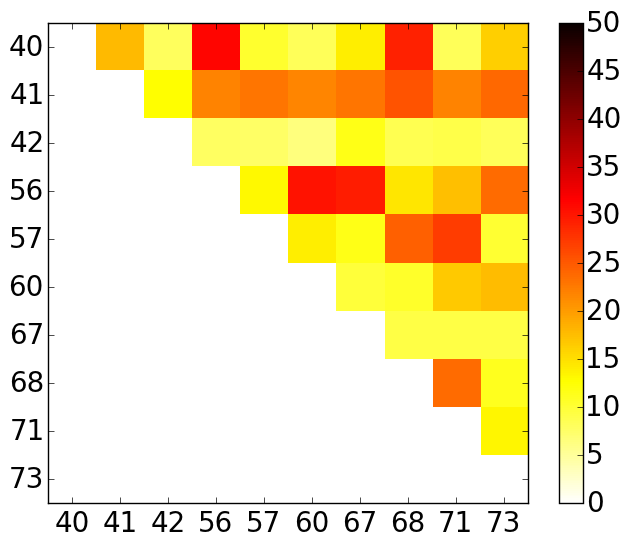
\includegraphics[width=35mm]{Chapters/dafx/figures/PEASSplots/OPS/NMF2.png} & 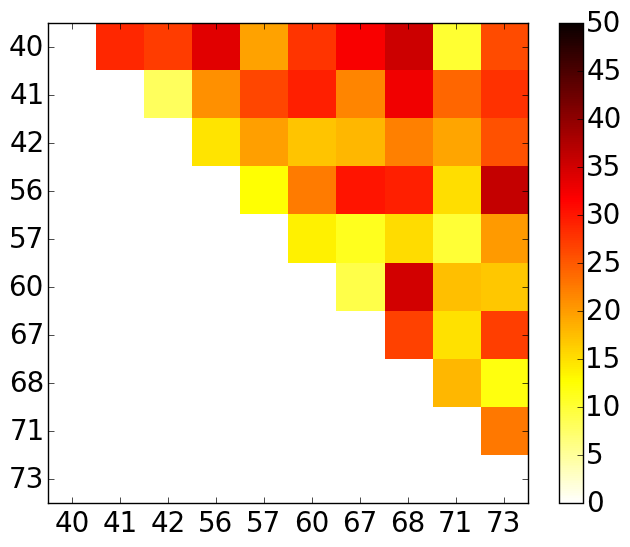
\includegraphics[width=35mm]{Chapters/dafx/figures/PEASSplots/OPS/NMF4.png} \\
    (a) NMF $K=2$ & (b) NMF $K=4$ \\[6pt]
        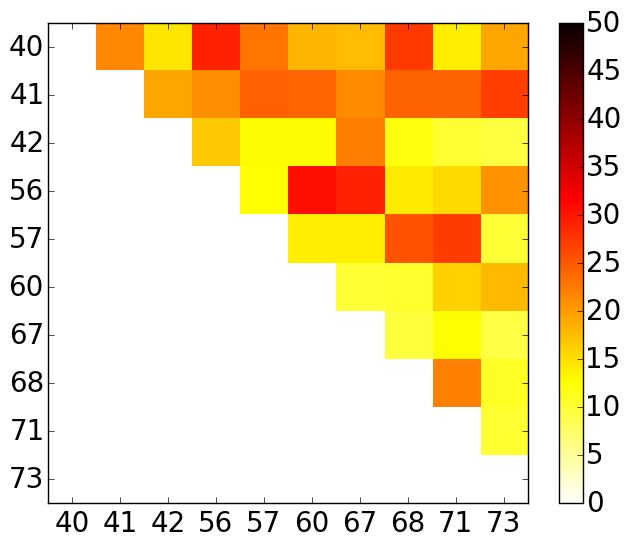
\includegraphics[width=35mm]{Chapters/dafx/figures/PEASSplots/OPS/NMFWARP2.png} & 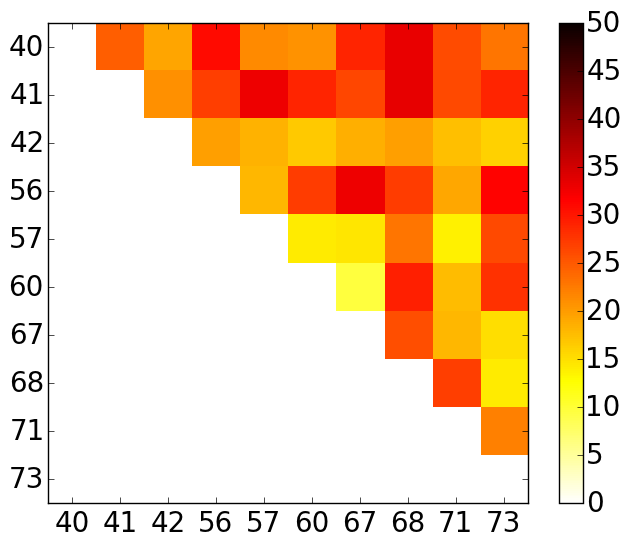
\includegraphics[width=35mm]{Chapters/dafx/figures/PEASSplots/OPS/NMFWARP4.png} \\
    (c) PVI-NMF $K=2$ & (d) PVI-NMF $K=4$ \\[6pt]
         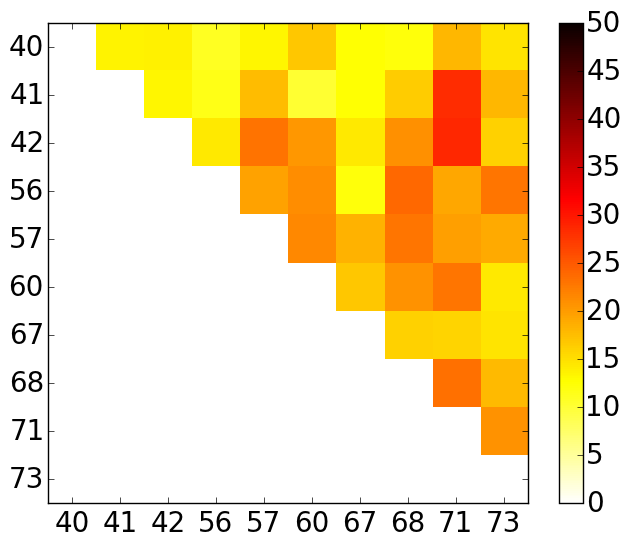
\includegraphics[width=35mm]{Chapters/dafx/figures/PEASSplots/OPS/NTF2.png} & 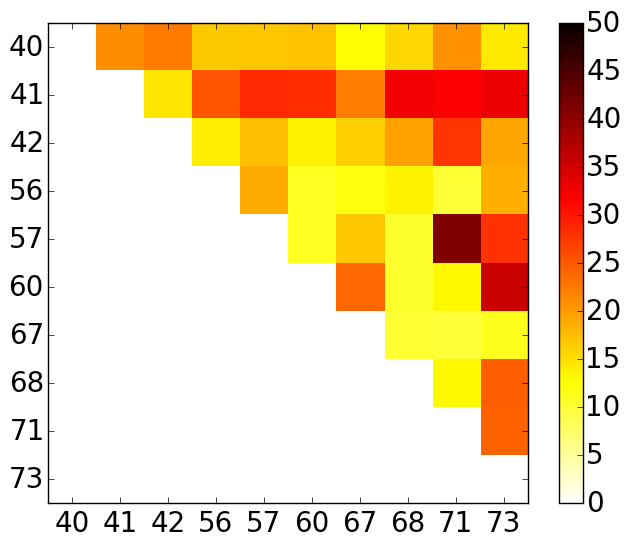
\includegraphics[width=35mm]{Chapters/dafx/figures/PEASSplots/OPS/NTF4.png} \\
    (e) MOD-NTF $K=2$ & (f) MOD-NTF $K=4$ \\[6pt]
\end{tabular}
\caption{Results of Overall Perceptual Score. Each matrix represents the mean OPS values for each individual mixture of two sources. The x and y axis represent the instrument IDs in General MIDI notation (See Table~\ref{tab:testset}).}
\label{tab:resultsmatrix}
\end{center}

\end{figure}

\begin{figure}[H]
    \centering
    \tiny
    \subfloat[Source 1]{
        \begin{tikzpicture}
            \begin{axis}[mystyle]
            \addplot [forget plot] graphics [xmin=0.5,xmax=1121.5,ymin=0.5,ymax=273.5] {Chapters/dafx/figures/src1-1.png};
            \end{axis}
        \end{tikzpicture}%
    }\hfill
    \subfloat[Source 2]{
        \begin{tikzpicture}
            \begin{axis}[mystyle]
            \addplot [forget plot] graphics [xmin=0.5,xmax=1121.5,ymin=0.5,ymax=273.5] {Chapters/dafx/figures/src2-1.png};
            \end{axis}
        \end{tikzpicture}%
    }

    \subfloat[Mixture]{
        \begin{tikzpicture}
            \begin{axis}[mystyle]
            \addplot [forget plot] graphics [xmin=0.5,xmax=1121.5,ymin=0.5,ymax=273.5] {Chapters/dafx/figures/mix-1.png};
            \end{axis}
        \end{tikzpicture}%
    }

    \subfloat[Mix. warped by Pitch 1]{
        \begin{tikzpicture}
            \begin{axis}[mystyle]
            \addplot [forget plot] graphics [xmin=0.5,xmax=1121.5,ymin=0.5,ymax=273.5] {Chapters/dafx/figures/mixwrpedsrc1-1.png};
            \end{axis}
        \end{tikzpicture}%
    }\hfill
    \subfloat[Mix. warped by Pitch 2]{
        \begin{tikzpicture}
            \begin{axis}[mystyle]
            \addplot [forget plot] graphics [xmin=0.5,xmax=1121.5,ymin=0.5,ymax=273.5] {Chapters/dafx/figures/mixwrpedsrc2-1.png};
            \end{axis}
        \end{tikzpicture}%
    }

    \subfloat[Target 1 warped]{
        \begin{tikzpicture}
            \begin{axis}[mystyle]
            \addplot [forget plot] graphics [xmin=0.5,xmax=1121.5,ymin=0.5,ymax=273.5] {Chapters/dafx/figures/src1wrped-1.png};
            \end{axis}
        \end{tikzpicture}%
    }\hfill
    \subfloat[Target 2 warped]{
        \begin{tikzpicture}
            \begin{axis}[mystyle]
            \addplot [forget plot] graphics [xmin=0.5,xmax=1121.5,ymin=0.5,ymax=273.5] {Chapters/dafx/figures/src2wrped-1.png};
            \end{axis}
        \end{tikzpicture}%
    }

    \subfloat[Target 1 unwarped]{
        \begin{tikzpicture}
            \begin{axis}[mystyle]
            \addplot [forget plot] graphics [xmin=0.5,xmax=1121.5,ymin=0.5,ymax=273.5] {Chapters/dafx/figures/src1unwarped-1.png};
            \end{axis}
        \end{tikzpicture}%
    }\hfill
    \subfloat[Target 2 unwarped]{
        \begin{tikzpicture}
            \begin{axis}[mystyle]
            \addplot [forget plot] graphics [xmin=0.5,xmax=1121.5,ymin=0.5,ymax=273.5] {Chapters/dafx/figures/src2unwarped-1.png};
            \end{axis}
        \end{tikzpicture}%
    }
    \caption{Example of pitch variation informed NMF in the warped domain. \textit{Time} is shown on horizontal axes. \textit{Frequency} is shown on vertical axes.}
    \label{fig:warpingdemo}
\end{figure}

%\newpage
% \nocite{*}
% \bibliographystyle{IEEEbib}
% \bibliography{DAFx14_tmpl} % requires file DAFx14_tmpl.bib


\chapter{Vocal/Accompaniment Separation}


\section{$F0$ informed Source Separation} % (fold)
\label{sec:method}

\kant[1-4]

\subsection{$F0$ Estimation Methods}

An estimate of the fundamental frequency $F0$ of a signal is required in various applications of audio and speech signal processing. $F0$ is often synonymously referred to as pitch which is a perceptual measure. In the past, a number of algorithms were presented to provide such estimates, with many of them being designed for specific applications. Some scenarios are targeted to extract the fundamental frequency of the predominant source~\cite{salamon2012melody} in a mixture of other sources. In other applications, algorithms are used to extract fundamental frequencies of multiple sources simultaneously present in a signal~\cite{klapuri2003multiple}. However, the most common scenario in many works is to extract the fundamental frequency of a monophonic and harmonic audio signal containing speech or music~\cite{talkin1995robust, boersma2002praat, de2002yin, resch, camacho2007swipe, tidhar2010high, christensen2007joint}.
%
The development of novel methods for fundamental frequency estimation, performing as well as earlier methods, such as the popular correlation based \textsc{YIN} algorithm~\cite{de2002yin}, has proven challenging. In a recent study~\cite{babacan2013comparative} it is stated that YIN still clearly performs best in terms of accuracy. Nevertheless, when using YIN or other block based algorithms, a frame length and a hop size have to be selected trading temporal resolution on one side against frequency accuracy and robustness on the other side.

Especially when the signal is polyphonic, the robustness is the most crucial aspect of a pitch estimator. In recent work from Mauch et al.~\cite{mauch2014pyin}, the robustness of the \textsc{YIN} algorithm is improved by probabilistic post-processing. However, besides robustness, there is a variety of use cases requiring high accuracy as well as high temporal resolution. Application in parametric audio coding~\cite{purnhagen2000hiln} requires the parameterization of pitch bends and vibratos. Furthermore, source separation algorithms aiming at the extraction of harmonic sources from the mixture can make use of an instantaneous $F0$ estimate~\cite{virtanen2008combining, stoterunison}. There are already contributions addressing the improvement of accuracy of $F0$ estimates such as~\cite{medan1991super} which introduced a non-integer similarity model or~\cite{christensen2007joint} which belongs to the group of parametric pitch estimators.

We propose to improve the output of already existing algorithms in terms of temporal resolution as well as accuracy by iterative time warping. Two other contributions already make use of time warping in the context of pitch estimation. Resch et al.~\cite{resch} proposed an instantaneous pitch estimation technique which optimizes a warping function that would lead to a constant pitch signal. Their optimization framework minimizes a cost function specifically targeted for speech signals. Azarov et al.\ have introduced an improved version of RAPT (called iRAPT1 and iRAPT2) which also uses time warping to some extent~\cite{azarov2012instantaneous} but misses an additional step as will be shown in Section~?.
Our main contribution is a time warping based refinement method that is applicable to any F0 estimate. Our method emphasizes the strengths of different estimators and thus can even help to improve their robustness. In the following, we will describe the refinement method (Section~?) and show the experimental evaluation and its results (Section~?).


Depending on the algorithm and application, there are several reasons why $F0$ estimators deliver a less than ideal performance. When the signal tested is not tonal --- like in unvoiced parts of speech --- a proper estimation is impossible. If the estimator is optimized on purely harmonic signals, inharmonicity or frequency jitter of the input signal will increase the estimation error. Many of these reasons will lead to errors on the coarse level of the estimate (like octave jumps). The fine level accuracy is mostly influenced by parameters like time and/or frequency resolution of the estimator. A signal containing rapid changes of the frequency or modulations like ``vibrato'' is therefore more affected regarding fine level error. To obtain a more accurate estimate, we propose to time warp the signal by using the coarse level estimate towards a more constant pitch. The underlying assumption here is that pitch estimators generally perform better the more constant the pitch is.
In this section, we formulate the mathematical background of the time warping and present our proposed method for obtaining a refined $F0$ estimate.
% \subsection{Initial $F0$ estimate}
% \label{sub:initial_estimate}

The first step is to calculate an initial $F0$ estimate by using an existing pitch estimator. Note that we later require the estimate to be defined for every input sample, thus $\Pitch[n]$ may require interpolation. In our pipeline, we use linear interpolation for all estimators. $F0$ estimators, like YIN~\cite{de2002yin}, also provide a measure of confidence $c[n]$.
\subsection{Time warping}
\label{sub:Refinement}

In this step, we apply \emph{time warping} which refers to a strictly monotonous mapping
of the natural or linear time scale $t$ to a warped time scale $\tau$ via a
mapping function $\tau=w(t)$.
The mapping between the two domains for the continuous time case then is:
\begin{equation}\label{eq:contWarpedTime}
\breve{x}(\tau)=x(w^{-1}(\tau)), \quad x(t)=\breve{x}(w(t))
\end{equation}
where $x(t)$ is the linear-time signal and $\breve{x}(\tau)$ is the warped-time signal.
For the discrete time case, the signals in both linear-time and warped-time domains are sampled
using a constant sample interval $T$. With sample indices $\nu$ and $n$ for the warped-time domain and linear time-domain respectively, the warping is performed by

\begin{align}
\breve{x}[\nu] &= x(\sigma[\nu]) & \textrm{ with } & \sigma[\nu] = w^{-1}(\nu T), \\
\intertext{and the inverse warping by}
x{}[n] &= \breve{x}(s[n]) & \textrm{ with } & s{}[n] = w(nT).
\end{align}

% \subsubsection{Warp contour}
% \label{subs:warp_contour}

In our application, the warp map $w(t)$ is constructed in such a way that the instantaneous changes in frequency of the signal in the linear time domain are minimized in the warped time domain. For this, we derive the map from an estimate of the fundamental frequency $F0$.

For processing, the actual information needed is not the absolute instantaneous fundamental frequency but only its change over time. This means that the warping contour can be derived from an algorithm which may differ from the actual $F0$ estimator.

The discrete time warp map $w[n]$ is the scaled sum of the relative
frequency contour (the \emph{warp contour}) $W[n]$:
\begin{equation}
w[n]=N \frac{\sum^n_{l=0}{W[l]}}{\sum^{N-1}_{k=0}{W[k]}}  \qquad 0\leq n<N,
\end{equation}
where $N$ being the number of samples of the signal under consideration.
As stated above the full warp map $w(t)$ is then obtained by linearly interpolating $w[n]$. From the requirements for the mapping function it follows that $W[n]$ has to be greater than zero for all $n$. In the case of a perfect $F0$ estimate, the signal warped with the resulting contour would have a constant $F0$ equal to the average $\bar{W}$.

In the scope of this work, the warping is applied globally over the full length of the signals under consideration. An optional confidence measure $c[n]$ can be incorporated for a processed version of the warping contour. This ensures that the warp contour has no discontinuities that result in additional artifacts after re-sampling. If the estimator does not provide such a measure, a separate voiced/unvoiced detection algorithm can be used. To obtain a warp contour $W[n]$ from an $F0$ estimate we propose the following steps: \textbf{(A)} initialize the warp contour with $F0$ estimate $W = \Pitch$, \textbf{(B)} find contour segments with high confidence, i.e. $c[n]$ exceeds a given threshold, \textbf{(C)} linearly connect the high confidence contour segments and \textbf{(D)} set start and end of warp contour to a constant value if confidence is below threshold. That way warping according to $F0$ is applied in the regions of high confidence without significantly affecting the gaps in-between.

\subsection{Source Extraction}
\kant[1-12]

%\vspace{-0.1cm}
\section{SiSEC Evaluation Campaigns}
\label{sec:evaluation}

\subsection{Organisation and Open Source Tools}
\label{ssec:background}

The problem of evaluating the quality of audio signals is a research topic of its own, which is deeply connected to psychoacoustics~\cite{zwicker13} and has many applications in engineering because it provides an objective function to optimize when designing processing methods. While mean squared error (MSE) is often used for mathematical convenience whenever an error is to be computed, it is a very established fact that MSE is not representative of audio perception~\cite{rix01,wang09}. For example, inaudible phase shifts would dramatically increase the MSE. Moreover, it should be acknowledged  that the concept of quality is rather application-dependent.

In the case of signal separation or enhancement, processing is often only a part of a whole architecture and a relevant methodology for evaluation is to study the positive or negative impact of this module on the overall performance of the system, rather than to consider it independently from the rest. For example, when embedded in an automatic speech recognition (ASR) system, performance of speech denoising can be assessed by checking whether it decreases word error rate~\cite{barker15}.

When it comes to music processing, and more particularly to lead and accompaniment separation, the evaluation of separation quality has traditionally been inspired by work in the audio coding community~\cite{recommendation2001MUSHRA,rix01} in the sense that it aims at comparing ground truth vocals and accompaniment with their estimates, just like audio coding compares the original with the compressed signal.

%\vspace{-0.2cm}
\subsection{Metrics}
\label{ssec:metrics}

As noted previously, MSE-based error measures are not perceptually relevant. For this reason, a natural approach is to have humans do the comparison. The gold-standard for human perceptual studies is the MUlti Stimulus test with Hidden Reference and Anchor (MUSHRA) methodology, that is commonly used for evaluating audio coding~\cite{recommendation2001MUSHRA}.

However, it quickly became clear that the specific evaluation of separation quality cannot easily be reduced to a single number, even when achieved through actual perceptual campaigns, but that quality rather depends on the application considered. For instance, karaoke or vocal extraction come with opposing trade-offs between isolation and distortion. For this reason, it has been standard practice to provide different and complementary metrics for evaluating separation that measure the amount of distortion, artifacts, and interference in the results.

While human-based perceptual evaluation is definitely the best way to assess separation quality~\cite{vincent062,cano11}, having computable objective metrics is desirable for several reasons. First, it allows researchers to evaluate performance without setting up costly and lengthy perceptual evaluation campaigns. Second, it permits large-scale training for the fine-tuning of parameters. In this respect, the Blind Source Separation Evaluation (BSS Eval) toolbox~\cite{fevotte05,vincent06} provides quality metrics in decibel to account for distortion (SDR), artifacts (SAR), and interferences (SIR). Since it was made available quite early and provides somewhat reasonable correlation with human perception in certain cases \cite{fox07,fox072} it is still widely used to this day.

Even if BSS Eval was considered sufficient for evaluation purposes for a long time, it is based on squared error criteria. Following early work in the area~\cite{kornycky08}, the Perceptual Evaluation of Audio Source Separation (PEASS) toolkit \cite{emiya10,emiya11,vincent122} was introduced as a way to predict perceptual ratings. While the methodology is very relevant, PEASS however was not widely accepted in practice. We believe this is for two reasons. First, the proposed implementation is quite computationally demanding. Second, the perceptual scores it was designed with are more related to speech separation than to music.
%Derry: Do we have space to add references to work which shows that PEASS fails to correlate with perception for many separation tasks?

Improving perceptual evaluation often requires a large amount of experiments, which is both costly and requires many expert listeners. One way to increase the number of participants is to conduct web-based experiments. In~\cite{cartwright16}, the authors report they were able to aggregate 530 participants in only 8.2 hours and obtained perceptual evaluation scores comparable to those estimated in the controlled lab environment.

Finally, we highlight here that the development of new perceptually relevant objective metrics for singing voice separation evaluation remains an open issue~\cite{gupta15}. It is also a highly crucial one for future research in the domain.

\subsection{Results SiSEC 2015}
\label{ssec:performance}

\kant[1-16]

%\vspace{-0.2cm}
\subsection{Results SiSEC 2016}
\label{ssec:performance}

In this section, we will discuss the performance of $23$ source separation methods evaluated on the DSD100, as part of the task for separating professionally-produced music recordings at SiSEC 2016. The methods are listed in Table~\ref{tab:systems}, along with the acronyms we use for them, their main references, a very brief summary, and a link to the section where they are described in the text. To date, this stands as the largest evaluation campaign ever achieved on lead and accompaniment separation. The results we discuss here are a more detailed report for SiSEC~2016~\cite{liutkus17}, presented in line with the taxonomy proposed in this paper.

\begin{table}[htbp]
	\centering
	\caption{Methods evaluated during SiSEC 2016.}
	\label{tab:systems}
	\begin{tabular}{|lll@{}l@{}|}
		\hline
		\textbf{Acronym} & \textbf{Ref.} & \textbf{Summary} & \textbf{Section}\\
		\hline
		HUA & \cite{huang12} & RPCA standard version & \ref{ssec:RPCA}\\
		\hline
		RAF1 & \cite{rafii13} & REPET standard version & \ref{ssec:methods_repet}\\
		RAF2 & \cite{liutkus12} & REPET with time-varying period & \\
		RAF3 & \cite{rafii12} & REPET with similarity matrix & \\
		KAM1-2 & \cite{liutkus15} & KAM with different configurations &\\
		\hline
		CHA & \cite{chan15} & RPCA with vocal activation information &\ref{ssec:methods_structureinformed}\\
		JEO1-2 & \cite{jeong17} &  $l_1$-RPCA with vocal activation information &\\
		\hline
		DUR & \cite{durrieu11} & Source-filter NMF &\ref{ssec:methods_sourcefilter}\\
		\hline
		OZE & \cite{salaun14} & Structured NMF with learned dictionaries & \ref{ssec:methods_datadriven_nmf}\\
		\hline
		KON & \cite{huang15} & RNN & \ref{ssec:methods_dnn} \\
		GRA2-3 & \cite{grais16} & DNN ensemble &\\
		STO1-2 & \cite{stoter16} & FNN on \textit{common fate} TF representation&\\
		UHL1 & \cite{Uhlich15} & FNN with context&\\
		\hline
		NUG1-4 & \cite{nugraha16} & FNN with multichannel information &\ref{sec:multichannel}\\
		UHL2-3 & \cite{uhlich17} & LSTM with multichannel information &\\
		\hline
		IBM & & ideal binary mask &  \\
		\hline
	\end{tabular}
\end{table}

%announcing the results and the webpage
The objective scores for these methods were obtained using BSS Eval and are given in Figure~\ref{fig:eval}. For more details about the results and for listening to the estimates, we refer the reader to the dedicated interactive website\footnote{\url{http://www.sisec17.audiolabs-erlangen.de}}.

\begin{figure*}[htbp]
	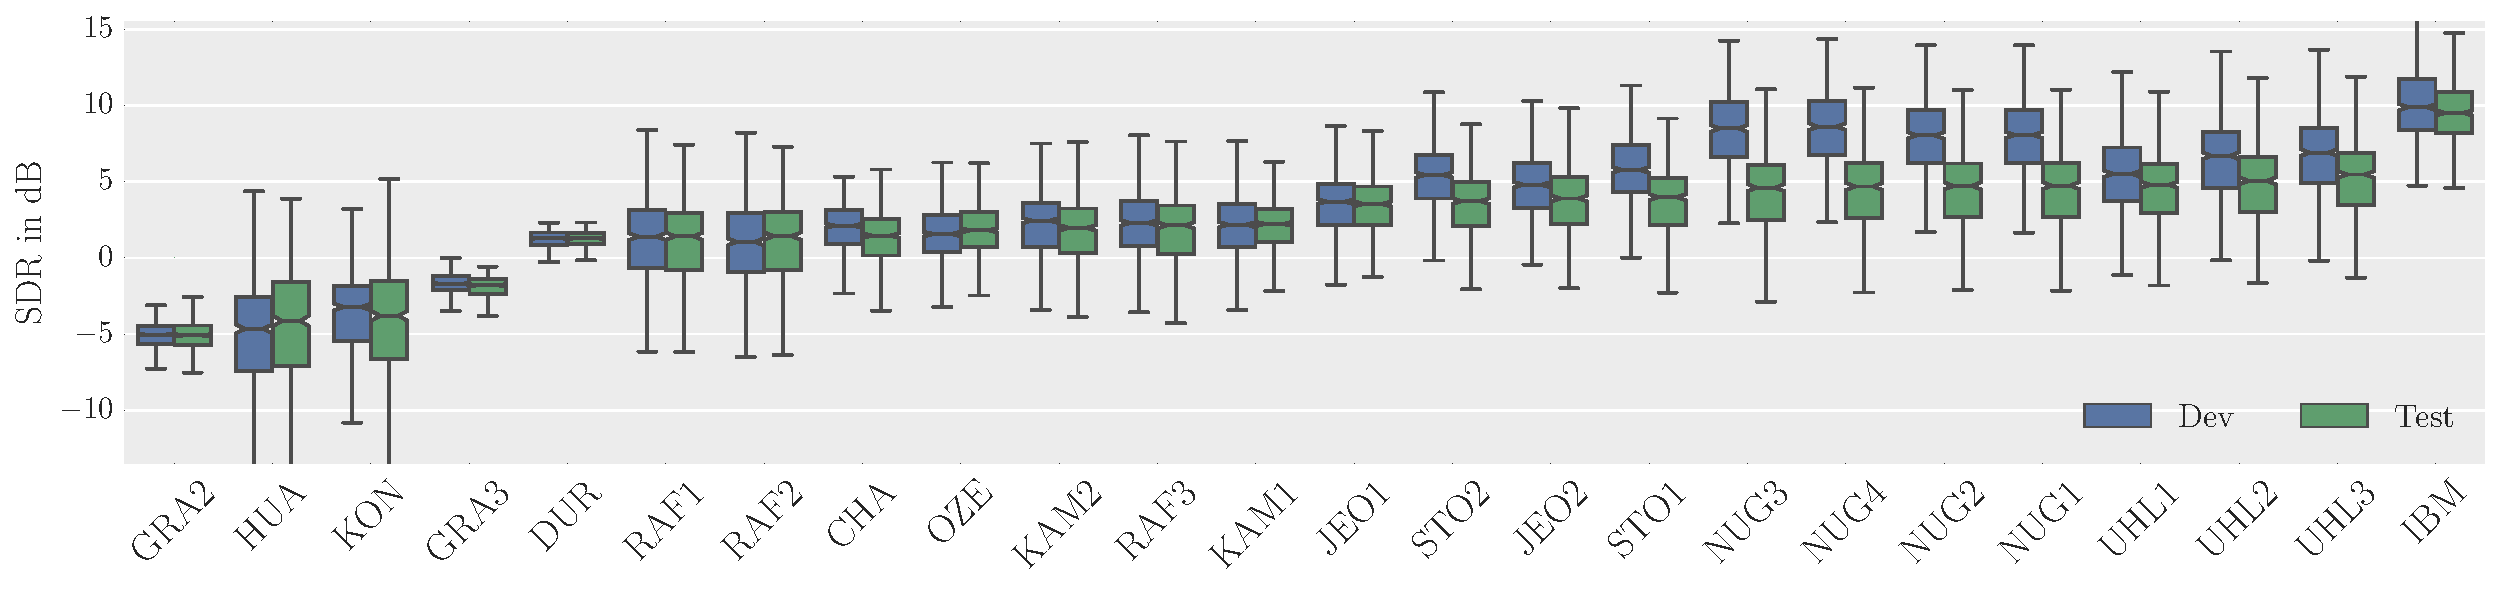
\includegraphics[width=\textwidth]{gfx/vocalsSDR.pdf}
	\caption{BSS Eval scores for the vocals and accompaniment estimates for SiSEC 2016 on the DSD100 dataset. Results are  shown for the \emph{test} set only. Scores are grouped as in Table~\ref{tab:systems} according to the section they are described in the text, indicated below each group.}
	\label{fig:eval}
\end{figure*}

%RPCA suffers from full-length recordings
As we first notice in Figure~\ref{fig:eval}, the HUA method, corresponding to the standard RPCA as discussed in Section~\ref{ssec:RPCA}, showed rather disappointing performance in this evaluation. After inspection of the results, it appears that processing full-length tracks is the issue there: at such scales, vocals also exhibit redundancy, which is captured by the low-rank model associated with the accompaniment. On the other hand, the RAF1-3 and KAM1-3 methods that exploit redundancy through repetitions, as presented in Section~\ref{ssec:methods_repet}, behave much better for full-length tracks: even if somewhat redundant, vocals are rarely as repetitive as the accompaniment. When those methods are evaluated on datasets with very short excerpts (e.g., MIR-1K), such severe practical drawbacks are not apparent.

%DUR also+non harmonic lead
Likewise, the DUR method that jointly models the vocals as harmonic and the accompaniment as redundant, as discussed in Section~\ref{ssec:methods_sourcefilter}, does show rather disappointing performance, considering that it was long the state-of-the-art in earlier SiSECs \cite{vincent12}. After inspection, we may propose two reasons for this performance drop. First, using full-length excerpts also clearly revealed a shortcoming of the approach: it poorly handles silences in the lead, which were rare in the short-length excerpts tested so far. Second, using a much larger evaluation set revealed that vocals are not necessarily well modeled by a harmonic source-filter model; breathy or saturated voices appear to greatly challenge such a model.

%RPCA informed by lead presence behaves well
While processing full-length tracks comes as a challenge, it can also be an opportunity. It is indeed worth noticing that whenever RPCA is helped through vocal activity detection, its performance is significantly boosted, as highlighted by the relatively good results obtained by CHAN and JEO.

%OZE could benefit from the new learning data
As discussed in Section~\ref{sec:datadriven-approaches}, the availability of learning data made it possible to build data-driven approaches, like the NMF-based OZE method which is available through the Flexible Audio Source Separation Toolbox (FASST) \cite{salaun14,ozerov12}. Although it was long state-of-the-art, it has been strongly outperformed recently by other data-driven approaches, namely DNNs. One first reason clearly appears as the superior expressive power of DNNs over NMF, but one second reason could very simply be that OZE should be trained anew with the same large amount of data.

%DNN are definitely performing awesomely
As mentioned above, a striking fact we see in Figure~\ref{fig:eval} is that the overall performance of data-driven DNN methods is the highest. This shows that exploiting learning data does help separation greatly compared to only relying on \textit{a priori} assumptions such as the harmonicity or redundancy. Additionally, dynamic models such as CNN or LSTM appear more adapted to music than FNN. These good performances in audio source separation go in line with the recent success of DNNs in fields as varied as computer vision, speech recognition, and natural language processing \cite{lecun15}.

%but it's clear that they benefit from smart ideas
However, the picture may be seen to be more subtle than simply black-box DNN systems beating all other approaches. For instance, exploiting multichannel probabilistic models, as discussed in Section~\ref{sec:multichannel}, leads to the NUG and UHL2-3 methods, that significantly outperform the DNN methods ignoring stereo information. In the same vein, we expect other specific assumptions and musicological ideas to be exploited for further improving the quality of the separation.

%weakness of metrics
One particular feature of this evaluation is that it also shows obvious weaknesses in the objective metrics. For instance, the GRA method behaves significantly worse than any other methods. However, when listening to the separated signals, this does not seem deserved. All in all, designing new and convenient metrics that better match perception and that are specifically built for music on large datasets clearly appears as a desirable milestone.

%IBM much better: room for improvement
In any case, the performance achieved by a totally informed filtering method such as IBM is significantly higher than that of any submitted method in this evaluation. This means that lead and accompaniment separation has room for much improvement, and that the topic is bound to witness many breakthroughs still. This is even more true considering that IBM is not the best upper bound for separation performance: other filtering methods such as \textit{ideal ratio mask}~\cite{liutkus15c} or multichannel Wiener filter~\cite{duong10} may be considered as references.

%importance of implementations and details, links to online ressources
Regardless of the above, we would also like to highlight that good algorithms and models can suffer from slight errors in their low-level audio processing routines. Such routines may include the STFT representation, the overlap-add procedure, energy normalization, and so on. Considerable improvements may also be obtained by using simple tricks and, depending on the method, large impacts can occur in the results by only changing low-level parameters. These include
%the length of each window, S: I think that this is not a trick. Various window sizes lead to different representations (sparser/disjoint) and they are a part of modelling the data. I believe we should keep it out.
the overlap ratio for the STFT, specific ways to regularize matrix inverses in multichannel models, etc. Further tricks such as the exponentiation of the TF mask by some positive value can often boost performance significantly more than using more sophisticated models. However, such tricks are often lost when publishing research focused on the higher-level algorithms. We believe this is an important reason why sharing source code is highly desirable in this particular application. Some online repositories containing implementations of lead and accompaniment separation methods should be mentioned, such as \textbf{nussl}\footnote{\url{https://github.com/interactiveaudiolab/nussl}} and \textbf{untwist} \cite{roma16}. In the companion webpage of this paper\footnote{\url{https://sigsep.github.io}}, we list many different online resources such as datasets, implementations, and tools that we hope will be useful to the practitioner and provide some useful pointers to the interested reader.


\section{Conclusion}

\part{Source Count Estimation}\label{pt:showcase}

\chapter{Perceptual Experiments}

\renewcommand{\rothead}[2][90]{\makebox[0mm][l]{\rotatebox{#1}{\makecell[c]{#2}}}}%
\renewcommand{\arraystretch}{1.4}

\newcommand*\node[1]{
\unitlength1ex
\begin{picture}(2.5,2.5)
\put(0.75,0.75){
	\circle{3}}
	\put(0.7,0.7){
		\makebox(0,0){#1}
	}
\end{picture}
}

\section{Introduction}
Decomposing music into its original audio sources can be a challenging task. Source separation methods can be analyzed how well they perform mathematically, but a human versus machine comparison is cumbersome because measurement of the human separation performance is problematic. One can easily evaluate if humans can detect the number of sources in a mixture of several sources. However, there are indications that even for this task, humans tend to fail if more than three sources are present at the same time \cite{huron89}. Therefore, we want to take a first step by designing an experiment where we focus on polyphonic music of inhomogeneous timbre, where the question is: What is the number of instruments humans can estimate correctly? Several results are addressed in this paper including a possible upper limit of the number of perceived instruments, but also if one can see significant differences in performance of musicians compared to non-musicians. Such results can be used in auditory modeling or as a pre-processing step for source separation algorithms.
This paper presents the results of an experiment, a detailed description of the stimuli and the statistical methods that were used.
\vspace{-1.0em}
\section{Related Work}
The perception of concurrent sound sources has been analyzed on different scales so far. Bregman's and McAdams' \cite{mcadams79} auditory stream theory can be seen as an analytical way of describing how sound events are perceived by the human auditory system. Unfortunately, it is difficult to model professionally produced music by auditory stream models because of its high complexity. As described by Wang \cite{wang2006} there exist several algorithms to estimate the actual number of sources. However, none of them is motivated to model the perceived number of musical sources. Kashino et. al \cite{kashino1995} addresses the questions for concurrent speakers in a ``cocktail party'' like environment and found an upper limit of three voices humans can perceive. When the focus shifts to musical instruments as sources, research has to take concepts from musicology into account. Huron \cite{huron89} was the first who addressed this question in 1989 at a musically meaningful level. Huron asked for the number of voices within a piece of music, where by voices in musicology one can define it as a line of sound or note events (See \cite{cambouropoulos2008voice} for further definitions). Huron determined by experimental results that the number of correctly identified voices is up to three. Later in 1996, Reuter \cite{reuter96} has analyzed how combinations of different instruments are perceived which sets the focus on different instrumentation and not on denumerability.
\vspace{-1.0em}
\section{Experiment}
For the purpose of gaining more knowledge in understanding the human perception of multiple present instruments, an experiment was conducted. Huron selected voices from organ pieces only. We wanted to address the more general case where voices are played by different instruments. Therefore we used a method between musicology and auditory stream analysis to address this question. As we set our focus mainly on comparison between musicians and non-musicians, our experiment was designed so that it respects the fact that the latter have only limited musical background.

Although it might be interesting to have direct comparison with Huron's experiment, we agree that expanding the methods to an inhomogeneous timbre case is error prone. One reason is that there is reasonable doubt about the non-musicians understandings in terms of how a voice is defined. This is why we choose a trade-off with a more simplified experiment where we asked for the number of instruments instead of voices. Also whereas Huron \cite{huron89}  excluded subjects from his experiment because of their lower performance, we compared the results of both groups.
\vspace{-1.0em}
\subsection{Stimuli}

The selection of music items is crucial for our experiment setup. Usually music recordings have no ground truth metadata available to determine the actual number of instruments. Using annotated music like that from the RWC database \cite{rwc} fulfills this requirement but lacks the possibility to remix, attenuate or suppress specific sources. This is important so that the experiment consists of equally grouped stimuli. Instead of the original RWC recordings, the annotated MIDI data itself was used as prototypes for the stimuli.

To make the counting task less ambiguous for the subjects, the instrumentation needs to be mostly constant during the music piece. Therefore we calculated an ``instrumental stationarity'' measure. The annotated MIDI files from \cite{rwc} were converted into piano roll representations for each instrument channel. This representation was then converted into a binary \emph{instrumentation activity matrix} $\mathbf{I}_{AM}\lbrack \mathbf{\underline{k}}_1 \vert \mathbf{\underline{k}}_2 \vert  ... \vert \mathbf{\underline{k}}_N \rbrack \in \{0,1\}$, where at each discrete time instant $i$ a vector $\mathbf{\underline{k}}_i$ indicates which instruments are active. The aim is then to select frames of length $N$ which are stationary by means of changes in instrumentation and activity. To get many items with a high instruments count, the maximum number of instruments within a frame was stored in a binary mask $\mathbf{\underline{k}}_{max}$ which was compared with all $\mathbf{\underline{k}}_{i=1...N}$ so that $(\vert\mathbf{\underline{k}}_{i} \oplus \mathbf{\underline{k}}_{max}\vert \leq 1) \lor (\mathbf{\underline{k}}_{i} = \underline{0})$. The resulting binary vector was smoothed with an averaging kernel of size $N$. By peak picking we got a list of possible candidates which contained a high stationarity in instrumentation.
Further the RWC files were filtered a priori to exclude items dominated by electronic instruments or singing voice. Table~\ref{tab:items} presents the selected 12 items representing pairs of one to six simultaneously present instruments. Each item is around seven seconds long. By cutting at note offsets we varied the lengths of the items to make it semantically more meaningful. Six items (notated as RM-C***) belong to the classical western music genre whereas the other items are of mixed genre.

The MIDI files were humanized randomly and rendered in a professional sequencer software utilizing state-of-the-art commercial sampling products. The rendered files were processed with convolutive reverb to better match the original recordings. Additionally equalization were applied to take loudness measures according to \textsc{EBU R128} recommendations into account. To avoid spatial cues every item was rendered to mono at 16 bit/44.1 kHz.

\begin{table}[h]
\center
\tiny
\begin{tabular}{c|r@{.}l|r@{.}l|l|l|l|l|l|l|l|l|l|l|l|l|l|l|l|l|l|l}
\toprule[1.5pt]

	\multicolumn{5}{l}{ } &
	\multicolumn{18}{c}{Instrument Name} \\

	RWC-MDB ID
	& \multicolumn{2}{c}{Start [s]}
	& \multicolumn{2}{c|}{Dur. [s]}
	& \rothead{Piano}
	& \rothead{Acoustic Guitar}
	& \rothead{Electric Guitar}
	& \rothead{Contrabass (pizz.)}
	& \rothead{Electric Bass}
	& \rothead{Violin}
	& \rothead{Viola}
	& \rothead{Violoncello}
	& \rothead{Contrabass}
	& \rothead{Trumpet}
	& \rothead{Trombone}
	& \rothead{French Horn}
	& \rothead{Tenor Sax}
	& \rothead{Oboe}
	& \rothead{Bassoon}
	& \rothead{Clarinet}
	& \rothead{Flute}
	& $\sum$ \\
	\midrule \hline
J021** & 46&5	& 6&6 & \cellcolor[gray]{0.9} $\times$& & & \cellcolor[gray]{0.9} $\times$& & & & & & \cellcolor[gray]{0.9} $\times$& & & & & & & & 3\\ \hline  \hline
C001 & 0&0 	& 9&0 & & & & & & & & & & & & & & & \cellcolor[gray]{0.9} $\times$& & & \multirow{2}{*}{1} \\
G047 & 35&3	& 8&3 & & & & & & & & \cellcolor[gray]{0.9} $\times$& & & & & & & & & &  \\ \hline
C016 & 0&9	& 7&6 & & & & & & & \cellcolor[gray]{0.9} $\times$ &\cellcolor[gray]{0.9} $\times$& & & & & & & & & & \multirow{2}{*}{2} \\
G068 & 132&4 & 6&6 & & & & & &\cellcolor[gray]{0.9} $\times$& & & & & & & & & & &\cellcolor[gray]{0.9} $\times$ & \\ \hline
C018 & 240&4	& 5&4 &\cellcolor[gray]{0.9} $\times$& & & & &\cellcolor[gray]{0.9} $\times$& & & & & &\cellcolor[gray]{0.9} $\times$& & & & & & \multirow{2}{*}{3} \\
G046 & 0&3	& 7&9 &\cellcolor[gray]{0.9} $\times$& & & & & & &\cellcolor[gray]{0.9} $\times$&\cellcolor[gray]{0.9} $\times$& & & & & & & & & \\ \hline
C013 & 5&6 	& 6&0 & & & & & &\cellcolor[gray]{0.9} $\times$&\cellcolor[gray]{0.9} $\times$&\cellcolor[gray]{0.9} $\times$& & & & & & & & &\cellcolor[gray]{0.9} $\times$ & \multirow{2}{*}{4} \\
G036 & 0&0	& 6&5 &\cellcolor[gray]{0.9} $\times$&\cellcolor[gray]{0.9} $\times$& & &\cellcolor[gray]{0.9} $\times$&\cellcolor[gray]{0.9} $\times$& & & & & & & & & & & & \\ \hline
C012 & 112&0 & 6&0 & & & & & &\cellcolor[gray]{0.9} $\times$&\cellcolor[gray]{0.9} $\times$&\cellcolor[gray]{0.9} $\times$&\cellcolor[gray]{0.9} $\times$& & & & & & & &\cellcolor[gray]{0.9} $\times$ & \multirow{2}{*}{5} \\
G037 & 67&1	& 7&0 &\cellcolor[gray]{0.9} $\times$&\cellcolor[gray]{0.9} $\times$& &\cellcolor[gray]{0.9} $\times$& & & & & & & & &\cellcolor[gray]{0.9} $\times$& & & &$\cellcolor[gray]{0.9} \times$ & \\ \hline
C001 & 147&8 & 6&0 & & & & & &\cellcolor[gray]{0.9} $\times$& & &\cellcolor[gray]{0.9} $\times$& & &\cellcolor[gray]{0.9} $\times$& &\cellcolor[gray]{0.9} $\times$&\cellcolor[gray]{0.9} $\times$&\cellcolor[gray]{0.9} $\times$& & \multirow{2}{*}{6} \\
G028 & 17&5 	& 6&5 &\cellcolor[gray]{0.9} $\times$& &\cellcolor[gray]{0.9} $\times$& &\cellcolor[gray]{0.9} $\times$& & & & &\cellcolor[gray]{0.9} $\times$&\cellcolor[gray]{0.9} $\times$& & & & & &\cellcolor[gray]{0.9} $\times$ & \\ \hline
\bottomrule[1.5pt]

\end{tabular}
\caption{Selected items from the RWC Music Database \cite{rwc}. Item \emph{J021**} is used as training item.}
\label{tab:items}
\end{table}

\subsection{Methods and Participants}

The experiment was attended by 62 participants, where half of them regularly play a musical instrument. They were asked to count how many different instruments they can hear. 12 items from the test set (Table~\ref{tab:items}) were played back in random order. The experiment was presented by a user interface depicted in Figure~\ref{fig:experiment_ui}. Except for the training item, every subject could play back each stimulus up to three times. Additionally they were asked to estimate how certain they were in their decision (ranged from \emph{uncertain} to \emph{very certain}).
\begin{figure}[h]
	\centering
		\fbox{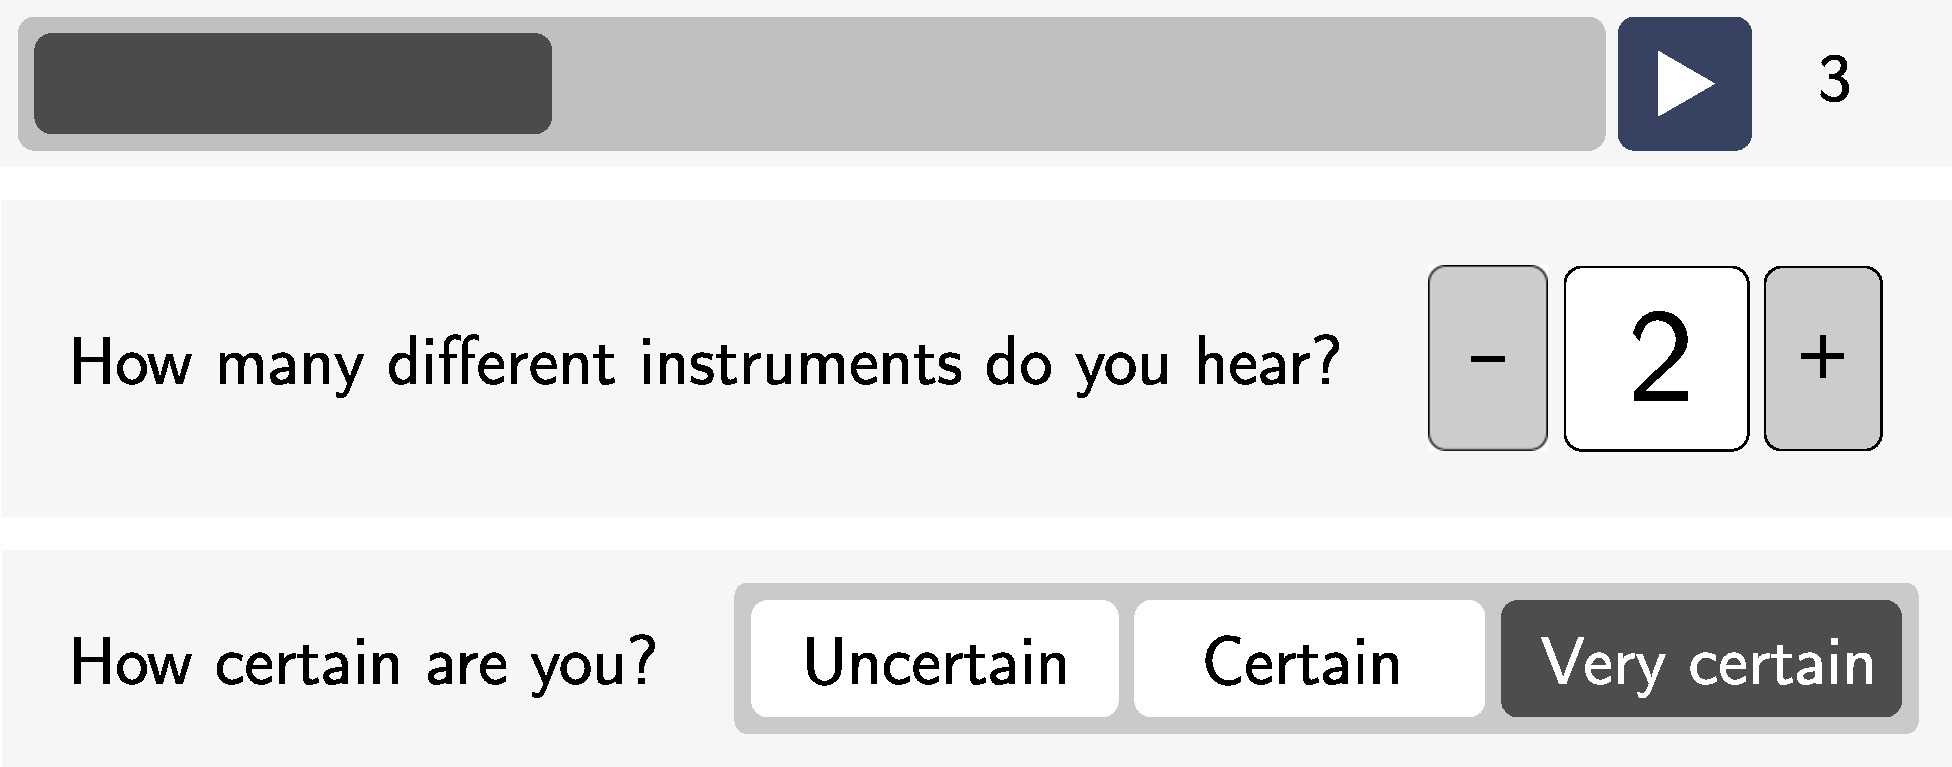
\includegraphics[width=3in]{Chapters/ica/images/userinterface.pdf}}
	\caption{Experiment User Interface}
	\label{fig:experiment_ui}
\end{figure}
Instead of a slider UI-element, the interface only features plus and minus buttons so that the subjects were not biased about the maximum number of instruments. Item \emph{J021**} had been selected as training item and was presented to the subjects during the introduction phase to make them familiar with the user interface. This trial also unveiled the number and name of the instruments within that piece. After they had read the introduction page, the subjects were asked to adjust the volume during the training example to their preference and leave the volume at that level for the duration of the experiment. The stimuli were presented on \textsc{Beyerdynamics DT770} headphones connected to a \textsc{RME Babyface}. The complete test took about 20 minutes on average for every participant.
\vspace{-1.0em}
\section{Results}

The independent variable $I(i)$ is the number of instruments of one music item $i$ where in this case $I(i) \in \{1,2,...,6\}$. $R(i,s)$ is defined as the number of instruments that are perceived and counted by subject $s$ for music item $i$. The dependent variable is the derived from the main subject response as $\Delta(i,s) = I(i) - R(i,s)$ and can also be transformed into a binary scale:
\begin{align*}
	E(i,s)&=\begin{cases}
		0 & \text{if $|\Delta| = 0 $ } \\
		1 & \text{if $|\Delta| > 0 $ .}\\
	\end{cases}
\end{align*}

As we want to address a possible upper bound for the number of instruments that humans are able to correctly count. The primary statistical null hypothesis ($H_1$) is stated in that the means of $\Delta$ and $E$\footnote{The fact that $E$ is dichotomous will lead to a mean value that equals to a probability of a binary distribution.}, grouped by the number of instruments, do not differ significantly. As we also want to test the between-groups performance of musicians versus non-musicians, we introduce another dependent variable $M(s) \in \{0,1\}$ of binary scale. This is stated in a secondary null hypothesis ($H_2$) where the means of $\Delta$ and $E$ are not significantly different between musicians and non-musicians.

The outcome of the experiment is shown in Table~\ref{tab:resultsoverall}. No subjects were screened from the results, although there are two cases where no valid response had been made. Results are grouped by items of $I$ instruments.

In general participants tended to perform worse for items with more than two instruments. The probability of correctly counting one instrument was 90.0\% whereas only one person out of 62 gave a correct response for an item with six instruments. In some cases the number of instruments does not correspond to the number of voices for every item. Items where an instrument plays more than one voice and voices which are played by more than one instrument. However most of the chosen instruments are monophonic so in our case this occured only for items where piano or guitar is present. Also we made sure that the number of total voices did not exceed the maximum number of instruments in that item. Voices being played by more than one instrument are called unisono, which is present in G068, that showed surprisingly good results.
The overall results of the means of $\Delta$ and $E$ are plotted in Figure~\ref{fig:meanerror}.
%!TEX root = ../ica_nautlib.tex
\begin{table}
\begin{center}
\tiny
\begin{tabular}{rrrrrrrrrrrrrrr}
\toprule[1.5pt]
\multicolumn{ 2}{c}{Responses} & \multicolumn{ 13}{c}{Stimuli of RWC-MDB items sorted by number of instruments} \\ 
 \cmidrule(r){1-2} \cmidrule(l){3-15}
 &  & \multicolumn{2}{c}{$I=1$} 
	& \multicolumn{2}{c}{$I=2$} 
	& \multicolumn{2}{c}{$I=3$} 
	& \multicolumn{2}{c}{$I=4$} 
	& \multicolumn{2}{c}{$I=5$} 
	& \multicolumn{2}{c}{$I=6$} 
	& \multicolumn{1}{l}{} \\ 
\cmidrule(r){3-4} \cmidrule(lr){5-6} \cmidrule(lr){7-8} \cmidrule(lr){9-10} \cmidrule(lr){11-12} \cmidrule(l){13-14}
Count & Subject Group &  C001-1 & G047 & C016 & G068 & C018 & G046 & C013 & G036 & C012 & G037 & C001-2 & G028 & n \\ 
\midrule

\multirow{2}{*}{$R=0$} & $M=0$ & 0 & 0 & 0 & 0 & 0 & 0 & 1 & 0 & 0 & 0 & 0 & 0 & 1 \\ 
 & $M=1$ & 0 & 1 & 0 & 0 & 0 & 0 & 0 & 0 & 0 & 0 & 0 & 0 & 1 \\ 
% & $\sum$ & \multicolumn{2}{r}{1} & \multicolumn{2}{r}{0} & \multicolumn{2}{r}{0} & \multicolumn{ 2}{r}{1} & \multicolumn{2}{r}{0} & \multicolumn{2}{r}{0} & 2 \\  

\midrule
\multirow{2}{*}{$R=1$} & $M=0$ & \cellcolor[gray]{0.9} 25 & \cellcolor[gray]{0.9} 30 & 7 & 6 & 0 & 0 & 1 & 1 & 2 & 0 & 1 & 0 & 73 \\ 
 & $M=1$ & \cellcolor[gray]{0.9} 26 & \cellcolor[gray]{0.9} 30 & 7 & 1 & 0 & 0 & 0 & 0 & 0 & 0 & 0 & 0 & 64 \\ 
% & $\sum$ & \multicolumn{2}{r}{\cellcolor[gray]{0.9} 111} & \multicolumn{2}{r}{21} & \multicolumn{2}{r}{0} & \multicolumn{ 2}{r}{2} & \multicolumn{ 2}{r}{2} & \multicolumn{2}{r}{1} & 137 \\  

\midrule
\multirow{2}{*}{$R=2$} & $M=0$ & 6 & 1 & \cellcolor[gray]{0.9} 21 & \cellcolor[gray]{0.9} 25 & 21 & 17 & 14 & 5 & 11 & 7 & 9 & 9 & 146 \\ 
 & $M=1$ & 5 & 0 & \cellcolor[gray]{0.9} 18 & \cellcolor[gray]{0.9} 29 & 6 & 4 & 3 & 3 & 3 & 0 & 3 & 0 & 74 \\ 
% & $\sum$ & \multicolumn{ 2}{r}{12} & \multicolumn{ 2}{r}{\cellcolor[gray]{0.9} 93} & \multicolumn{ 2}{r}{48} & \multicolumn{ 2}{r}{25} & \multicolumn{ 2}{r}{21} & \multicolumn{ 2}{r}{21} & 220 \\  

\midrule
\multirow{2}{*}{$R=3$} & $M=0$ & 0 & 0 & 2 & 0 & \cellcolor[gray]{0.9} 8 & \cellcolor[gray]{0.9} 14 & 11 & 20 & 11 & 17 & 13 & 13 & 109 \\
 & $M=1$ & 0 & 0 & 4 & 1 & \cellcolor[gray]{0.9} 18 & \cellcolor[gray]{0.9} 27 & 19 & 14 & 10 & 11 & 16 & 8 & 128 \\ 
% & $\sum$ & \multicolumn{ 2}{r}{0} & \multicolumn{ 2}{r}{7} & \multicolumn{ 2}{r}{\cellcolor[gray]{0.9} 67} & \multicolumn{ 2}{r}{64} & \multicolumn{ 2}{r}{49} & \multicolumn{2}{r}{50} & 237 \\  

\midrule
\multirow{2}{*}{$R=4$} & $M=0$ & 0 & 0 & 1 & 0 & 2 & 0 & \cellcolor[gray]{0.9} 4 & \cellcolor[gray]{0.9} 4 & 7 & 5 & 6 & 8 & 37 \\
 & $M=1$ & 0 & 0 & 2 & 0 & 7 & 0 & \cellcolor[gray]{0.9} 9 & \cellcolor[gray]{0.9} 13 & 15 & 18 & 5 & 22 & 91 \\ 
% & $\sum$ & \multicolumn{ 2}{r}{0} & \multicolumn{ 2}{r}{3} & \multicolumn{ 2}{r}{9} & \multicolumn{ 2}{r}{\cellcolor[gray]{0.9} 30} & \multicolumn{ 2}{r}{45} & \multicolumn{ 2}{r}{41} & 128 \\  

\midrule
\multirow{2}{*}{$R=5$} & $M=0$ & 0 & 0 & 0 & 0 & 0 & 0 & 0 & 1 & \cellcolor[gray]{0.9} 0 & \cellcolor[gray]{0.9} 2 & 2 & 1 & 6 \\
 & $M=1$ & 0 & 0 & 0 & 0 & 0 & 0 & 0 & 1 & \cellcolor[gray]{0.9} 2 & \cellcolor[gray]{0.9} 2 & 6 & 1 & 12 \\ 
% & $\sum$ & \multicolumn{ 2}{r}{0} & \multicolumn{ 2}{r}{0} & \multicolumn{ 2}{l}{} & \multicolumn{ 2}{r}{2} & \multicolumn{ 2}{r}{\cellcolor[gray]{0.9} 6} & \multicolumn{ 2}{r}{10} & 18 \\  

\midrule
\multirow{2}{*}{$R=6$} & $M=0$ & 0 & 0 & 0 & 0 & 0 & 0 & 0 & 0 & 0 & 0 & \cellcolor[gray]{0.9} 0 & \cellcolor[gray]{0.9} 0 & 0 \\
 & $M=1$ & 0 & 0 & 0 & 0 & 0 & 0 & 0 & 0 & 1 & 0 & \cellcolor[gray]{0.9} 1 & \cellcolor[gray]{0.9} 0 & 2 \\ 
% & $\sum$ & \multicolumn{ 2}{r}{0} & \multicolumn{ 2}{r}{0} & \multicolumn{ 2}{r}{0} & \multicolumn{ 2}{r}{0} & \multicolumn{ 2}{r}{1} & \multicolumn{ 2}{r}{\cellcolor[gray]{0.9} 1} & 2 \\ 
\midrule 
 &  $\sum$& \multicolumn{12}{c}{62 participants, 744 responses} & \\    
\midrule[1pt]
\multirow{3}{*}{Error Probability} & $M=0$ & 0.19 & 0.03 & 0.32 & 0.19 & 0.74 & 0.55 & 0.87 & 0.87 & 1.00 & 0.94 & 1.00 & 1.00 & 0.64 \\ 
 & $M=1$ & 0.16 & 0.03 & 0.42 & 0.06 & 0.42 & 0.13 & 0.71 & 0.58 & 0.94 & 0.94 & 0.97 & 1.00 & 0.53 \\ \cmidrule(r){3-4} \cmidrule(lr){5-6} \cmidrule(lr){7-8} \cmidrule(lr){9-10} \cmidrule(lr){11-12} \cmidrule(lr){13-14} \cmidrule(l){15-15}
 & $\sum$ & \multicolumn{2}{c}{0.10} & \multicolumn{ 2}{c}{0.25} & \multicolumn{2}{c}{0.46} & \multicolumn{2}{c}{0.76} & \multicolumn{ 2}{c}{0.95} & \multicolumn{2}{c}{0.99} & 0.59 \\  
\midrule
\multirow{3}{*}{Mean($\Delta = I-R$)} & $M=0$ & -0.19 & -0.03 & 0.10 & 0.19 & 0.61 & 0.55 & 1.48 & 1.03 & 2.26 & 1.94 & 3.03 & 2.97 & 1.16 \\ 
 & $M=1$ & -0.16 & 0.03 & -0.03 & 0.00 & -0.03 & 0.13 & 0.81 & 0.61 & 1.39 & 1.29 & 2.45 & 2.23 & 0.73 \\ \cmidrule(r){3-4} \cmidrule(lr){5-6} \cmidrule(lr){7-8} \cmidrule(lr){9-10} \cmidrule(lr){11-12} \cmidrule(lr){13-14} \cmidrule(l){15-15}
 & $\sum$ & \multicolumn{2}{c}{-0.09} & \multicolumn{2}{c}{0.06} & \multicolumn{2}{c}{0.31} & \multicolumn{2}{c}{0.98} & \multicolumn{ 2}{c}{1.72} & \multicolumn{2}{c}{2.67} & 0.94 \\ 
\bottomrule[1.5pt]
\end{tabular}
\end{center}
\caption{Experiment results by subjects. Gray background indicates correct responses.}
\label{tab:resultsoverall}
\end{table}


\begin{figure}[h]
\begin{minipage}{0.5\textwidth}
\begin{tabular}{c}
	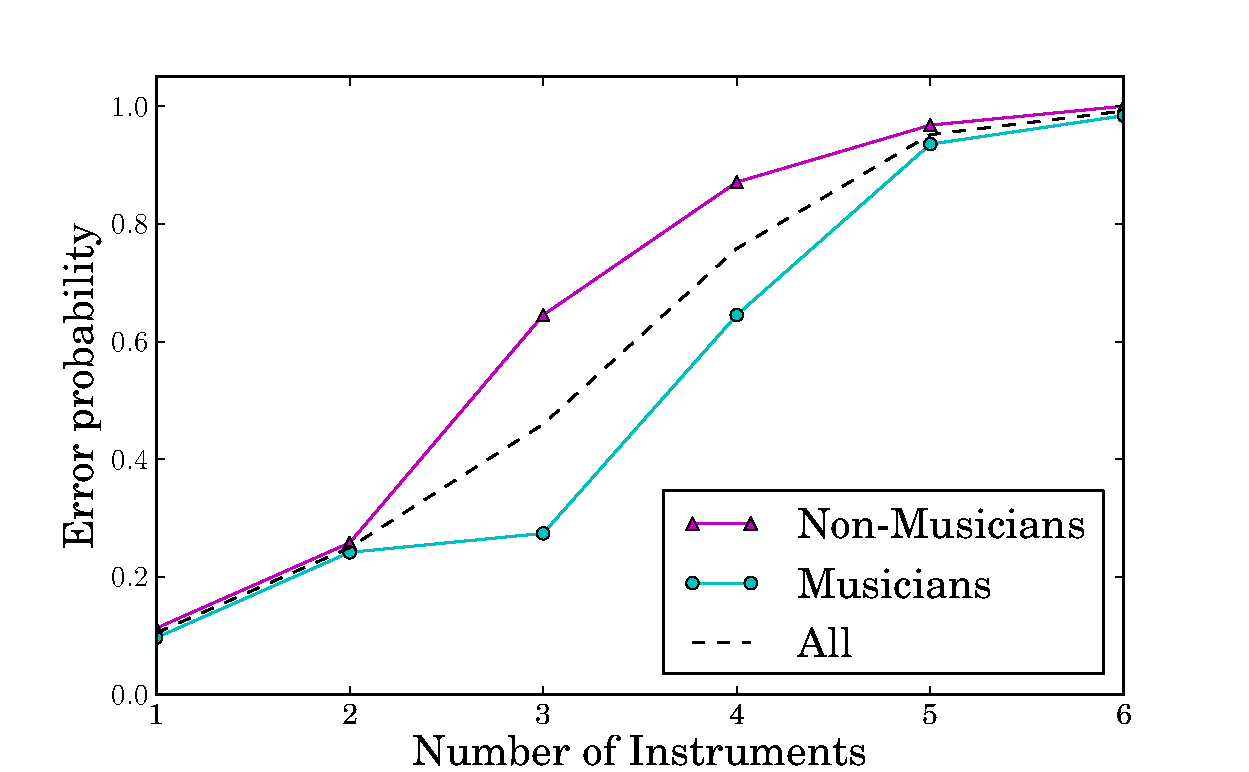
\includegraphics[width=\textwidth]{Chapters/ica/images/error_means.pdf}
\end{tabular}
\end{minipage}
%\hfill
\begin{minipage}{0.5\textwidth}
\begin{tabular}{c}
	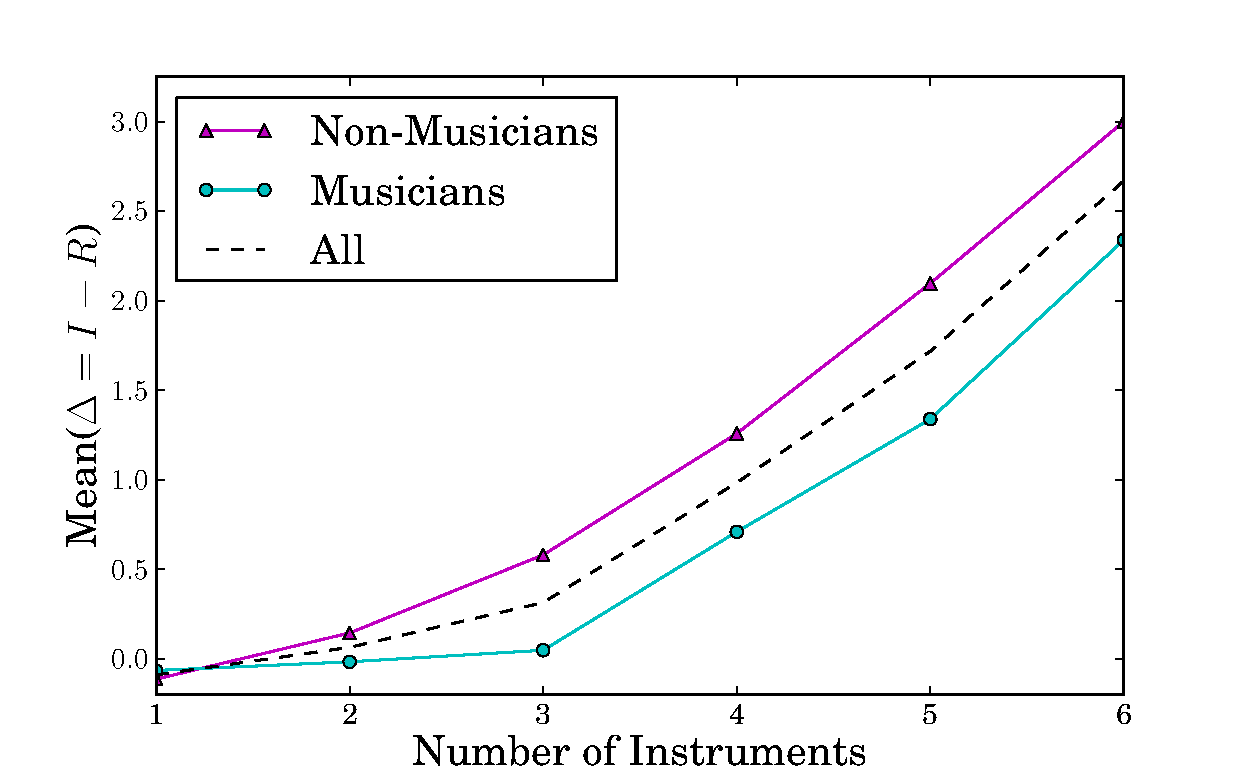
\includegraphics[width=\textwidth]{Chapters/ica/images/error_diff.pdf}
\end{tabular}
\end{minipage}
\caption{Error probability (left) and Mean of $\Delta = I-R$ (right) categorized by the number of instruments.}
\label{fig:meanerror}
\end{figure}
\vspace{-1.0em}

\subsection{Underestimation}

We confirm \cite{huron89} that the most common error is the underestimation of one instrument, although this accounts only for 43 \% of the responses in our experiment. Only in one case $\Delta$ is negative (overestimation) which is item C016, a ``Clarinet Quintet in A major by Wolfgang Amadeus Mozart (K.581. 1st mvmt)'' where we have excluded the solo clarinet part and two strings. Still, the remaining sound seems to be so similar to that of a quartet that musicians tended to hear ``phantom'' instruments.
\vspace{-1.0em}

\subsection{Self-Evaluation}

Figure~\ref{fig:certainty} shows the results of the subjects certainty grouped by instrument count. Although the rate of ``very certain'' responses drops down to 11.3\% for items with six instruments the rate of ``certain'' responses is still as high as 43.5\%. When we take $\Delta$ into account we find a significant linear correlation between $\Delta$ and certainty where 0 is uncertain and 2 is very certain (Pearson's $r = -0.227$ at the $p=0.05$ level).

\begin{figure}[h]
	\centering
		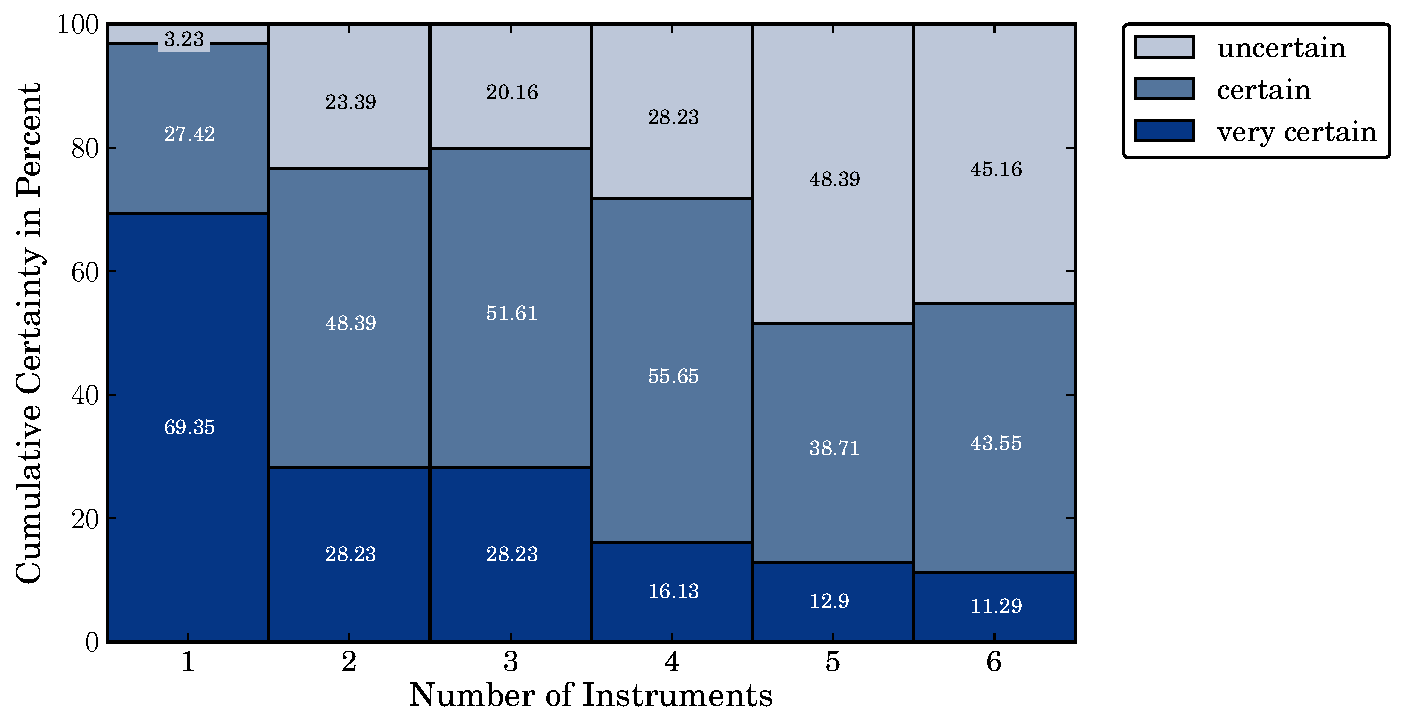
\includegraphics[height=2.5in]{Chapters/ica/images/certainty.pdf}
	\caption{Responses for certainty of subjects by number of instruments}
	\label{fig:certainty}
\end{figure}

\subsection{Main Effects}

Rejecting the null hypotheses ($H_1$ and $H_2$) requires further statistical methods. One reason is that the dependent variables $\Delta$ and $E$ have different scales. We will show that both variables qualify to reject our hypotheses.
As $E$ is dichotomous we focus on $\Delta$ first which can be classified as an interval scaled variable. To show differences between means of two or more groups, usually One-Way-ANOVA tests are applied. ANOVA tests expect independent normally distributed variables and homogeneity of the variances in each group. However both the Kolmogorov--Smirnov test of normal distribution and Levene's test to determine the homogeneity of group variances fail. In such cases variables scaled like $\Delta$ could be transformed so that the boundaries are straightened out. A typically used $arcsin(\sqrt{\Delta})$ transformation was applied to $\Delta$ resulting in slightly higher $p$ values but still not statistically significant. Although ANOVA is known to be robust enough to run the tests against non-normal distributed cases and unequal variances, the significance levels of the results are doubtful. Therefore we choose to run a non-parametric test. The Kruskal--Wallis test can be applied even if the data is not normally distributed. However it has to be run on a slightly modified hypothesis which compares the medians of groups instead of the means. The Kruskal--Wallis test allows to reject both modified hypotheses (asymptotic $p = 0.000$, $\chi^2 = 499636$, $df=5$). As mentioned by \cite{fagerland2009} it may be crucial for the Kruskal--Wallis test to be run on groups with differently shaped distributions. This may not be assured in the case of $\Delta$ as the skewness highly increases for $I \geq 3$. Although the significance of the test has to be treated with caution, the median is a good indicator of a possible upper limit. The overall medians for all groups are plotted in Figure~\ref{fig:median} where one can see that three instruments are a possible upper bound.

\begin{figure}[h]
	\centering
	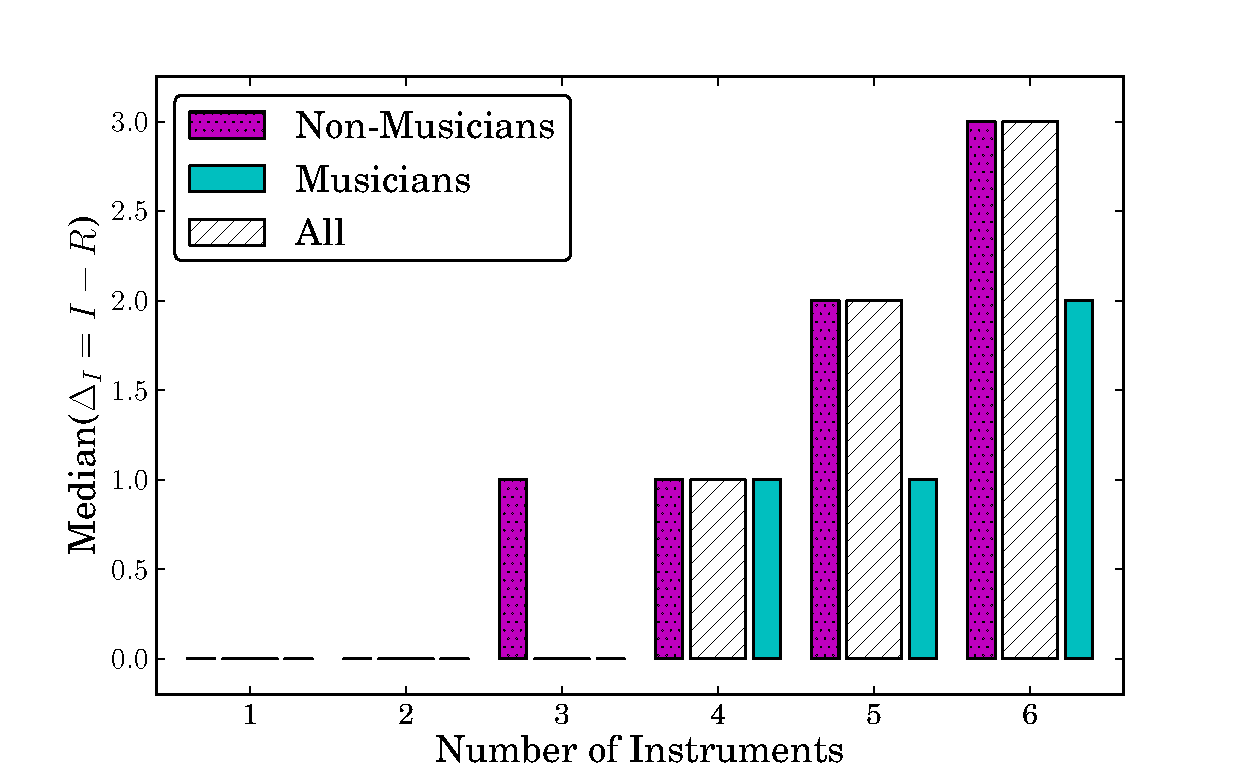
\includegraphics[width=0.6\textwidth]{Chapters/ica/images/diff_medians.pdf}
\caption{Median of $\Delta$ categorized by the number of instruments}
\label{fig:median}
\end{figure}

The reason why an ANOVA is not recommended to be run on $E$ is because it is a categorical variable. Like described in \cite{jaeger2008} this leads to problems which can be avoided by using a binary regression model that turns the mean of $E$ into a an binomial distributed probability. Whereas in standard linear models like ANOVA the output variable will be modeled by a linear equation, in a so called \emph{binary logit regression} the output will be modeled by \emph{log linear} values. By including the main factors $I$ and $M$ we set up a \emph{Generalized Linear Model} (GLM)
\begin{equation}
	logit(E) =  \text{Intercept} + x_1 \text{I} + x_2 \text{M} .
	\label{eq:logit_main}
\end{equation}
A test of the main effects is statistically significant ($\chi^2$ = $437418$, $p < 0.000$, $df = 6$) so that both null hypotheses ($H_1$ and $H_2$) can be rejected. The significance of both effects is shown in Table~\ref{tab:glm_logit} whereas parameter estimates and Wald values of the calculated model are shown in Table~\ref{tab:glm_logit_parameter_estimates}. The intercept represents a constant calculated offset within the regression.

\begin{table}
\center
\scriptsize
\begin{tabular}{cccccc}
\toprule[1.5pt]
Parameter & B & Std. Error & Wald $\chi^2$ & df & Sig. \\
\midrule
(Intercept) & -4.456 & 1.0067 & 19.590 & 1 & .000\\
$M=0$ & -.910 & .2147 & 17.977 & 1 & .000\\
$M=1$ & 0 & . & . & . &  \\
$I=1$ & 7.136 & 1.0507 & 46.131 & 1 & .000\\
$I=2$ & 6.061 & 1.0291 & 34.691 & 1 & .000\\
$I=3$ & 5.081 & 1.0228 & 24.677 & 1 & .000\\
$I=4$ & 3.715 & 1.0274 & 13.076 & 1 & .000\\
$I=5$ & 1.841 & 1.0892 & 2.856 & 1 & .091\\
$I=6$ & 0 & . & . & . & .\\
\bottomrule[1.5pt]
\end{tabular}
\caption{Parameter Estimates for GLM model. Missing values are represented by the Intercept.}
\label{tab:glm_logit_parameter_estimates}
\end{table}

The tests we introduced in the last section show that there is a significant difference in the error probability for groups of different instrumentation but also for musicians versus non-musicians. A pairwise comparison test based on the mean differences reveals where these differences are located. Regarding the error probability of different instrument counts, the pairwise comparison test reveals that nearly all groups show significant mean differences between each other, which was the expected result. However, by calculation using the logit GLM model shown in equation~\ref{eq:logit_main} we found that there are two groups of items of five and six instruments (mean difference $0.04$, std. error = $0.019$, $df = 1$, $p = 0.055$) that did not show any significant difference. For both groups the error probability is close to 100\%.
\subsection{A gap of one instrument between musicians and non-musicians}
To investigate the difference in performance between musicians and non-musicians a pairwise comparison between those two groups was run. Overall musicians perform about 20\% better throughout the test (mean difference = $0.18$, std. error = $ 0.0044$, $df = 1$, $p=0.000$). We do not know what caused these differences as the level of professionalism had not been surveyed. Also 37 \% of the musicians additionally had experience in audio engineering due to their profession. Further to look at possible interaction effects between the number of instruments and the groups of musicians and non-musicians we adapted our logit equation to
\begin{equation}
	logit(E) =  \text{Intercept} + x_1 \text{I} + x_2 \text{M} + x_3 \text{M}\times\text{I} .
	\label{eq:logit_interactions}
\end{equation}
We then reran the GLM analysis selecting only items of three and four instruments. This avoids quasi-complete separation in the logit regression model which is caused by low variances in the error probability for items of $I \in \{1,2,5,6\}$. The model effects of the subset of items are shown in Table~\ref{tab:glm_logit_34}.
\begin{table}
\center
\scriptsize
\begin{minipage}[b]{0.45\textwidth}\centering
	\begin{tabular}{rccc}
	\toprule[1.5pt]
	Source    & Wald $\chi^2$ & df & p \\
	\midrule
	Intercept & 22.643 & 1 & 0.000 \\
	I & 185.359	& 5 & 0.000 \\
	M & 17.977 & 1 & 0.000 \\
	& & & \\
	\bottomrule[1.5pt]
	\end{tabular}
	\caption{Tests of Model Effects of dependent variable $E$ }
    \label{tab:glm_logit}
\end{minipage}
\hfill
\begin{minipage}[b]{0.45\textwidth}
	\begin{tabular}{rccc}
	\toprule[1.5pt]
	Source    & Wald $\chi^2$ & df & p \\
	\midrule
	Intercept & 12.434 & 1 & 0.000 \\
	I & 22.742	& 1 & 0.000 \\
	M & 22.742 & 1 & 0.000 \\
	M$\times$I	& 0.184 & 1 & 0.668 \\
	\bottomrule[1.5pt]
	\end{tabular}
	\caption{Tests of Model Effects of dependent variable $E$ for a subset of items with $I \in \{3,4\}$}
    \label{tab:glm_logit_34}
\end{minipage}
\end{table}

\begin{figure}[h]
	\centering
	\scriptsize
	\begin{tikzpicture}[node distance=2cm]
		\draw [-,thick] (0,5*1.25) node (yaxis) [left] {$ $}
	        |- (7,0.75) node (xaxis) {$ $};

		\draw (-1.1, 5) node[left,rotate=90] {Error~Probability};

		\draw (1,-0.2+0.75) -- (1,0+0.75) node[below=4pt] {musician};
		\draw (5.5,-0.2+0.75) -- (5.5,0+0.75) node[below=4pt] {non-musician};

	%	\draw (-0.1, 0) -- (0.1, 0) node[left=4pt] {$0\%$};
		\draw (-0.1, 1.3710*1.25) -- (0.1, 1.3710*1.25) node[left=4pt] {$0.27$};
		\draw (-0.1, 3.2258*1.25) -- (0.1, 3.2258*1.25) node[left=4pt] {$0.65$};
		\draw (-0.1, 4.3548*1.25) -- (0.1, 4.3548*1.25) node[left=4pt] {$0.87$};
	%	\draw (-0.1, 5*1.25) -- (0.1, 5*1.25) node[left=4pt] {$100\%$};

		\draw[dashed,style={color=black!35}] (0, 1.3710*1.25) -- (1.5, 1.3710*1.25) node[left=4pt] {};
		\draw[dashed,style={color=black!35}] (0, 3.2258*1.25) -- (1.5, 3.2258*1.25) node[left=4pt] {};
		\draw[dashed,style={color=black!35}] (0, 4.3548*1.25) -- (5.5, 4.3548*1.25) node[left=4pt] {};

		\GraphInit[vstyle=Normal]
		\tikzset{EdgeStyle/.style={}}
		\tikzset{colorstyle/.style={
			shape= circle,
			line width = 1pt,
			draw = black,
			fill = #1!30}
		}

		\Vertex[L=3,x=1,y=1.3710*1.25,style={colorstyle=red,line width = 4pt}] {3M}
		\Vertex[L=4,x=1,y=3.2258*1.25,style={colorstyle=blue,line width = 2pt}] {4M}
		\Vertex[L=3,x=5.5,y= 3.2258*1.25,style={line width = 4pt}] {3N}
		\Vertex[L=4,x=5.5,y=4.3548*1.25,style={colorstyle=green, draw = black!0,line width = 0}] {4N}

		\Edge[label=$0.23$,style={color=black!50}](3N)(4N)
		\Edge[label=$0.37$,style={color=black!50}](3N)(3M)

		\Edge[label=$0.23$,style={color=black!50}](4N)(4M)
		\Edge[label=$0.37$,style={color=black!50}](4M)(3M)
		\Edge[label=$0.60$,style={color=black!50}](3M)(4N)
		\Edge[label=$0.00$,style={color=red, line width = 2pt}](3N)(4M)

		\end{tikzpicture}
		\caption{Pairwise comparison between interaction of Musician/Non-Musician and the number of instruments (labeled in nodes). The costs between nodes indicates the mean differences between groups. The red/bold line indicates that is there is no significant difference at the $p=0.005$ level}
		\label{fig:graph}
\end{figure}
The interaction of Musician$\times$Instruments is not significant on a $p=0.05$ level in general and a pairwise comparison test reveals two groups of equal probability. The pairwise comparisons are depicted in Figure~\ref{fig:graph}. The red vertex indicates there is no significant difference in the error probability for the group of musicians in items with four instruments compared to non-musicians in items of three instruments. Therefore a gap in the error probability of one instrument between those two groups becomes apparent.
\section{Conclusion}
This paper shows that counting the number of instruments in a music item is a difficult task for humans. A new experiment with 62 participants was conducted to address the question of how many instruments one can estimate correctly.
In this experiment, the focus was set on stimuli of inhomogeneous timbre and also mixed genre. By comparing musicians to non-musicians, we revealed that there is a significant difference in performance. Particularly this gap is most prominent for items of three and four instruments. Furthermore, for all stimuli (ranging from one to six instruments) we see that musicians performed about 20\% better than non-musicians. The experiment shows an assumed upper limit for items with more than three instruments. Our results are closely related to a previous experiment which focused on voices instead of instruments.
This work can be used as a basis to define target functions for related research in auditory modeling. Future work could address different groups of items to reveal if certain instrumentations or compositions influence the results.

% \bibliographystyle{jasanum}
%\bibliographystyle{jasaauthyear}

% -----------------------------------------------
% Template for ISMIR 2013
% (based on earlier ISMIR templates)
% -----------------------------------------------
%
% \usepackage{ismir2013,amsmath,cite}
% \usepackage{graphicx}
% %custom packages
% \usepackage{footnote}
% \usepackage{color}
% \usepackage{multirow}
% \usepackage{xcolor}
% \usepackage{multirow}
% \usepackage{makecell}
% \usepackage{textcomp}
% \usepackage{subfigure}
% \usepackage{amssymb}
% \usepackage{booktabs}
% \usepackage{siunitx}
% \usepackage{colortbl,array}
% \usepackage{url}
% \makeatletter
% \g@addto@macro{\UrlBreaks}{\UrlOrds}
% \makeatother
% \usepackage{tikz}
% \usetikzlibrary{arrows}
% \usepackage{pgfplots}
% \pgfplotsset{compat=1.8}
% \usepgfplotslibrary{statistics}
% \usetikzlibrary{patterns}
% \usepackage{anyfontsize}

Internet experiments in the fields of music perception and music information retrieval are becoming more and more popular. However, not many Internet experiments are compared to laboratory experiments, the consequence being that the effect of the uncontrolled Internet environment on the results is unknown.
In this paper the results of an Internet experiment with 1168 participants are compared to those of the same experiment with 62 participants but previously conducted in a controlled environment. The comparison of the Internet and laboratory results enabled us to make a point on whether the Internet can be used for our experiment procedure. The experiment aimed to investigate the listeners ability to correctly estimate the number of instruments being played back in a given excerpt of music. The participants listened to twelve short classical and pop music excerpts each composed using one to six instruments. For each music excerpt the participants were asked how many instruments they could hear and how certain they were about their estimation.
%
\section{Introduction}\label{sec:introduction}
%For developing source separation algorithms, knowing the maximum number of instruments humans are able to identify could be helpful. E.~g. this number can be used as a target value which the algorithm has to outperform when the algorithm has to be better than the auditory system of humans.

In psychoacoustics, a sequence of sounds grouped by the auditory system is known as an ``auditory stream'' which was coined by Bregman and Campbell\cite{Bregman1971}. In the past decades, a lot of experimental work related to ``auditory streams'' has been done\cite{Bregman1990}. A majority of these experiments were psychoacoustically motivated, e.~g. the stimuli used were mostly of simple type like sinusoids or noises. Especially from a psychoacoustic point of view, music is a very complex sound signal which contains high-level information (e.~g. instrumentation and song lyrics). When listening to music, this high-level information is also mentally processed by humans. For developing auditory models, it could be helpful to know the maximum number of instruments humans are able to estimate when listening to music.

For many types of music perception experiments such as estimating the number of instruments, it is essential that the selected participants represent a large population. As recent research in cross-cultural music perception and cognition reveals: The perception of music is dependent on the origin of people\cite{Stevens2012}. Besides the cultural background, other aspects like their profession might have an influence when estimating the number of instruments being played back, e.~g. musicians might recognize instruments much more easily since they are in touch with instruments in their everyday life. One of the advantages of Internet experiments (also called web-based experiments or web experiments) is that it is easier to gather participants with different backgrounds and from different regions than in laboratory experiments. For a summary of benefits and disadvantages of Internet experiments see \cite{Reips2002}. In music perception a major argument against Internet experiments is that there is no control about the environment. With the spreading of mobile devices with Internet connections this argument becomes more apparent, since the environment of the participants can range from a quiet place at home to a noisy place outside.

By comparing the results of the Internet experiment presented in this paper to the results of the same experiment but previously conducted in a controlled environment\cite{Stoter2013}, we contribute to answering the research question, whether the Internet can be used for experiments in music perception. Furthermore, subpopulations like headphones-users and loudspeaker-users are examined whether they lead to more reliable responses.

\section{Related Work}\label{sec:related_work}
The ability of estimating the number of instruments is probably related to the ability of auditory stream segregation. An overview of auditory stream segregation in general is given by Bregman\cite{Bregman1990} and Wang and Brown\cite{wang2006}.

In 1989, Huron conducted a musically motivated experiment related to stream segregation\cite{Huron1989}. In his experiment he asked the participants for the number of voices in excerpts of organ music. Huron defined a voice as a single ``line'' of sound, more or less continuous, that maintains a separate identity in a sound field or musical texture (an overview of voice definitions is given by Cambouropoulos\cite{Cambouropoulos2008}). Huron came to the conclusion that the number of correctly identified voices is up to three. Based on Hurons work, we carried out an experiment where we asked musicians and non-musicians how many instruments they could hear in short pieces of music\cite{Stoter2013}. In contrast to Huron we addressed a more general case where voices are played by different instruments and not only by organ. In Huron's experiment the responses of the participants were time-varying for each stimulus. Another difference is that in Huron's experiment all six participants except one had a musical background whereas our experiment was also attended by a large group of non-musicians.

It has been becoming more and more popular to use the Internet for experiments in music or auditory perception. One of the first auditory experiments were conducted by Welch and Krantz\cite{Welch1996} in 1996. A web experiment related to MIREX tasks using \emph{Amazon Mechanical Turk} has been conducted by Lee \cite{lee2010}. An experiment with a large attendance was done by Salganik~\textit{et~al.}\cite{Salganik2006} in 2006. They had over 14.000 participants and examined the social influence on participants in an artificial music market. An overview of recent Internet experiments is given by Reips\cite{Reips2012}.

\section{Method}\label{sec:method}

\subsection{Stimuli}\label{sec:stimuli}
For the stimuli generation, MIDI files of music pieces from the RWC database\cite{rwc} were selected. The MIDI files were modified so that each file has a specific number of instruments being played back. Since the number of instruments being played back had to be as constant as possible, a so-called ``instrumental stationarity'' for each music piece was calculated. The ``instrumental stationarity'' is a measure that shows whether all instruments are played the whole time for a given start position and length. See \cite{Stoter2013} for the detailed equation of ``instrumental stationarity'' and more information about the stimuli generation. The RWC files were manually filtered a priori to exclude items dominated by lead instruments or singing voices. From the remaining items thirteen excerpts of MIDI files were selected with the help of the ``instrumental stationarity'' having one to six simultaneously playing instruments. Table~\ref{table:items} shows the selected excerpts including their instrumentation. The duration of each excerpt is around seven seconds. By cutting at note offsets we varied the lengths of the excerpts to make them semantically more meaningful. Six items (notated as C0**) belong to the classical Western music genre whereas the other items are of mixed genre.
\renewcommand{\arraystretch}{1.1}
\begin{table}[htb]
\center
\tiny
\begin{tabular}{c|r@{.}l|r@{.}l|p{3.8cm}|c}
\toprule[1.5pt]
RWC~ID & \multicolumn{2}{c}{Start~[s]} & \multicolumn{2}{c}{Dur.~[s]} & Instrumentation & $\sum$\\
\midrule
\hline
J021 & 46 & 5 & 6 & 6 & Piano, Contrabass~(pizz.) and Trumpet & 3\\
\hline
\hline
C001 & 0&0 & 9&0 & Bassoon & 1  \\
G047 & 35&3 & 8&3 & Violoncello & 1 \\
\hline
C016 & 0&9 & 7&6 & Viola and Violoncello & 2\\
G068 & 132&4 & 6&6 & Violin and Flute &  2\\
\hline
C018 & 240&4 & 5&4 & French~Horn, Piano and Violin & 3\\
G046 & 0&3 & 7&9 & Contrabass, Piano and Violoncello & 3\\
\hline
C013 & 5&6 & 6&0 & Flute, Viola, Violin and Violoncello & 4\\
G036 & 0&0 & 6&5 &  Acoustic~Guitar, Electric~Bass, Piano  and Violin & 4\\
\hline
C012 & 112&0 & 6&0 & Contrabass, Flute, Viola, Violin and  Violoncello & 5\\
G037 & 67&1 & 7&0 & Acoustic~Guitar, Contrabass~(pizz.), Flute, Piano and Tenor~Sax & 5\\
\hline
C001 & 147&8 & 6&0 & Bassoon, Clarinet, Contrabass, French~Horn, Oboe and Violin & 6\\
G028 & 17&5 & 6&5 & Electric~Bass, Electric~Guitar, Flute, Piano, Trombone and Trumpet & 6\\
\hline
\bottomrule[1.5pt]
\end{tabular}
\renewcommand{\arraystretch}{1}
\caption{Selected items from the RWC~Music~Database\cite{rwc}. Item \emph{J021} was used as training item.}
\label{table:items}
\end{table}
The MIDI excerpts were humanized and rendered by a sequencer software utilizing state-of-the-art commercial sampling products into WAV files. The rendered files were processed with convolutive reverb to match the original recordings. In informal listening tests the quality of the renderings was evaluated. In addition, participants did not give negative feedback about the artificialness of the items during the laboratory experiment. Additionally a loudness normalization was applied according to EBU-R128\cite{EBU2011}. To avoid spatial cues the files were downmixed to mono at 16~bit/44.1~kHz.

\subsection{Participants}
Participation in the experiment was done by visiting the experiment's website\footnote{{\scriptsize\url{http://www.audiolabs-erlangen.com/experiments/wice/}}}. The experiment was promoted in mailing lists, forums, social networks and by personal invitations. Most of the forums and mailing lists were audio-related. No material incentive was given to participants. For motivating the participants a high score was added to the experiment.

In total 1310 website visitors attended the experiment. We identified 115 of them as participants who did the experiment more than once by using a browser fingerprinting method (for more details in browser fingerprinting, see \cite{Eckersley2010}). In this case, only the first trial is used in the results analysis. Our browser fingerprinting method created a hash value by using the visitor's browser settings, e.~g. screen resolution and installed plugins. In addition, we excluded 27 participants since they gave at least one non-serious response. We defined responses with zero instruments (25~participants) and responses with more than 12 instruments (two participants) as invalid. After the screening we had 1168 valid participants.

The participants were asked by a questionnaire whether they have a professional background in audio, play at least one instrument (including singing) and are familiar with listening tests. Detailed information about the participants are described in Table~\ref{table:info_participants}.
\begin{table}[htb]
\center
\scriptsize
\renewcommand{\arraystretch}{1.2}
%\begin{tabular}{cr@{.}lr@{.}lr@{.}l}
\begin{tabular*}{0.45\textwidth}{c r@{ }l r@{ }l r@{ }l r@{ }l r@{ }l}
\toprule[1.5pt]
Total & \multicolumn{2}{c}{Age group} & \multicolumn{2}{c}{Musician} & \multicolumn{2}{c}{Professional} & \multicolumn{2}{c}{Headphones} \\
\midrule
1168 &  0  & [0-12]  & -   &  	   & -   &       & -   &       \\
 	 \cline{2-9} \rule{0pt}{10pt}
     & 110 & [13-19] & 74  & [yes] & 12  & [yes] & 5   & [yes] \\
     &     &         &	   &       &     &       & 7   & [no]  \\
     &     &   		 &     &       & 62  & [no]  & 30  & [yes] \\
     &     &         &	   &       &     &       & 32  & [no]  \\
     &     &   		 & 36  & [no]  & 0   & [yes] & -   &       \\
     &     &         &	   &       &     &       & -   &       \\
     &     &   		 &     &       & 36  & [no]  & 17  & [yes] \\
     &     &         &	   &       &     &       & 19  & [no]  \\
     \cline{2-9} \rule{0pt}{10pt}
     & 889 & [20-39] & 463 & [yes] & 128 & [yes] & 81   & [yes] \\
     &     &         &	   &       &     &       & 47   & [no]  \\
     &     &   		 &     &       & 335 & [no]  & 154  & [yes] \\
     &     &         &	   &       &     &       & 181  & [no]  \\
     &     &   		 & 426 & [no]  & 46  & [yes] & 31   & [yes] \\
     &     &         &	   &       &     &       & 15   & [no]  \\
     &     &   		 &     &       & 380 & [no]  & 164  & [yes] \\
     &     &         &	   &       &     &       & 216  & [no]  \\
     \cline{2-9} \rule{0pt}{10pt}
     & 143 & [40-59] & 98 & [yes] & 32  & [yes] & 22   & [yes] \\
     &     &         &	  &       &     &       & 10   & [no]  \\
     &     &   		 &    &       & 66  & [no]  & 31   & [yes] \\
     &     &         &	  &       &     &       & 35   & [no]  \\
     &     &   		 & 45 & [no]  & 8   & [yes] & 5    & [yes] \\
     &     &         &	  &       &     &       & 3    & [no]  \\
     &     &   		 &    &       & 37  & [no]  & 17   & [yes] \\
     &     &         &	  &       &     &       & 20   & [no]  \\
     \cline{2-9} \rule{0pt}{10pt}
     & 26  & [60+]   & 13 & [yes] & 6   & [yes] & 3    & [yes] \\
     &     &         &	  &       &     &       & 3    & [no]  \\
     &     &   		 &    &       & 7   & [no]  & 4    & [yes] \\
     &     &         &	  &       &     &       & 3    & [no]  \\
     &     &   		 & 13 & [no]  & 2   & [yes] & 2    & [yes] \\
     &     &         &	  &       &     &       & 0    & [no]  \\
     &     &   		 &    &       & 11  & [no]  & 5    & [yes] \\
     &     &         &	  &       &     &       & 6    & [no]  \\
\bottomrule[1.5pt]
\end{tabular*}
\caption{Information about the participants.}
\renewcommand{\arraystretch}{1}
\label{table:info_participants}
\end{table}

\subsection{Materials and Apparatus}\label{sec:materials}
The main functionality of the experiment's website was written in HTML5 and JavaScript. The website was tested for all major web browsers and optimized for mobile devices and desktop computers. The default file format for the stimuli was WAV. Since some browsers (e.~g. Internet Explorer) did not support WAV, MP3 (encoded with \SI{256}{kbits/s} CBR with Fraunhofer Encoder) was used as alternative file format. The alternative file format was only used when WAV was not supported by the browser.

\subsection{Procedure}\label{sec:procedure}
The experiment started on February the 15th, 2013 and lasted until March the 15th, 2013. %TODO the data was captured between... and ...

At first, participants filled out a short questionnaire. They were asked which audio setup they are using, whether they regularly play any musical instruments or do singing, have a background in professional audio, are familiar with listening tests and which age group they belong to.

After filling out the questionnaire, the participants did a short training. The purpose of the training was to familiarize the participants with the user interface and to give them the option to adjust the volume. The training had one stimulus with three instruments being played. The instruments were piano, bass and trumpet. The participants were told on the training page how many and which instruments are played back. During the training it was possible to listen to the stimulus unlimited times.

Followed by the training, the participants had to estimate the number of instruments being played in twelve stimuli. The experiment question was ``How many different instruments do you hear?". Participants could listen to each stimulus up to three times. In addition, they were asked how certain they were in their response. They could choose between ``uncertain'', ``certain'' and ``very certain''. The user interface is shown in Figure~\ref{figure:user_interface}.

\begin{figure}[htb]
	\centering
		\fbox{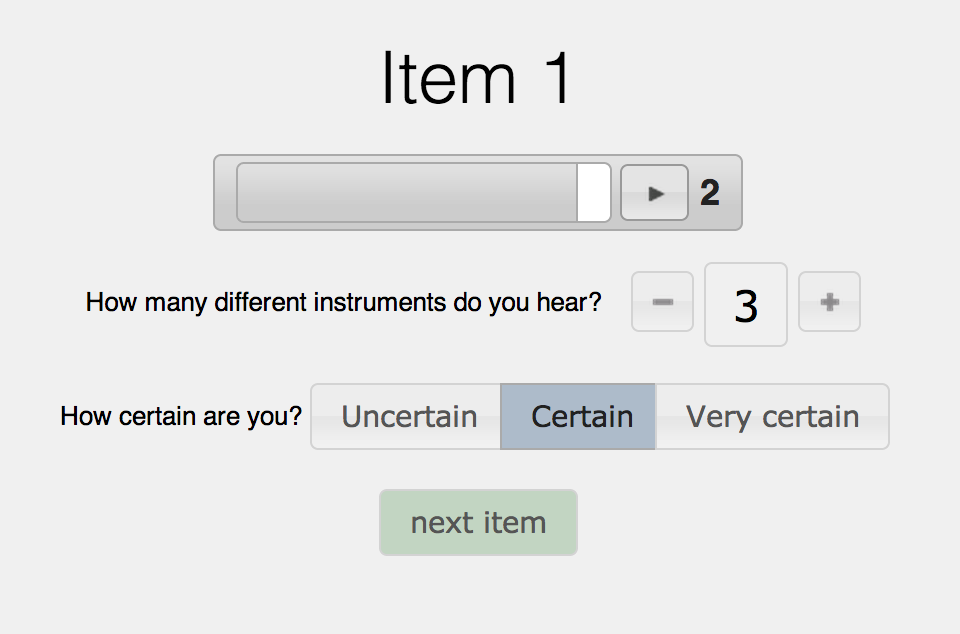
\includegraphics[width=2.8in]{Chapters/ismir/user_interface.png}}
	\caption{Experiment User Interface.}
	\label{figure:user_interface}
\end{figure}

After the participants estimated the number of instruments for all twelve stimuli, they were given a score based on their performance. Besides their personal score, a percentile rank showed how each participant performed compared to all the other participants.

\section{Results}\label{sec:results}

The independent variables are the number of instruments being played back ($\textit{Num}_{\mathrm{Inst}}$), whether a participant is musical ($\textit{Musical}$), professional in audio ($\textit{Professional}$) and which setup was used ($\textit{Setup}$). A participant is defined as musical ($\textit{Musical} = true$) when he or she is regularly playing an instrument (including singing). The same applies to being professional ($\textit{Professional} = true$) which is set when the participant responded that he or she is a professional in audio. The responses for the setup used can either be headphones ($\textit{Setup} = \textrm{`}headphones\textrm{'}$) or loudspeaker ($\textit{Setup} = \textrm{`}loudspeaker\textrm{'}$). The dependent variable is the participant's estimation of the number of instruments being played back ($\textit{Resp}$). A correct estimation is defined as
\begin{equation}
\label{equation:response_correct}
\textit{Resp}_{\mathrm{Correct}} =
\begin{cases}
0 & \text{if } \text{\textit{Num}}_{\mathrm{Inst}} \neq \text{\textit{Resp}}
\\
1 & \text{if } \text{\textit{Num}}_{\mathrm{Inst}} = \text{\textit{Resp}}
\end{cases}
\mathrm{.}
\end{equation}
Table~\ref{table:responses} shows the responses of the participants for all stimuli.
\tabcolsep=5.5pt
\begin{table}[t]
\tiny
\begin{tabular}{p{1cm}ccccccc}
\toprule[1.5pt]
 & \multicolumn{ 7}{c}{$\textit{Num}_{\mathrm{Inst}}$} \\
  \cmidrule(l){2-8}
 $\textit{Resp}$ & $I=1$ & $I=2$ & $I=3$ & $ I=4$ & $I=5$ & $I=6$ & n \\

 \midrule
 $R=1$ & \cellcolor[gray]{0.9} 2025 & 373 & 5 & 18 & 13 & 12 & 2446 \\
 \midrule
 $R=2$ & 298 & \cellcolor[gray]{0.9} 1642 & 810 & 736 & 451 & 382 & 4319 \\
 \midrule
 $R=3$ & 12 & 277 & \cellcolor[gray]{0.9} 1343 & 1145 & 1093 & 1069 & 4939 \\
 \midrule
 $R=4$ & 1 & 43 & 158 & \cellcolor[gray]{0.9} 386 & 645 & 680 & 1913 \\
 \midrule
 $R=5$ & 0 & 1 & 18 & 48 & \cellcolor[gray]{0.9} 120 & 155 & 342 \\
 \midrule
 $R=6$ & 0 & 0 & 1 & 3 & 12 & \cellcolor[gray]{0.9} 30 & 46 \\
 \midrule
 $R>6$ & 0 & 0 & 1 & 0 & 2 & 8 & 11 \\

 \midrule
 & \multicolumn{7}{c}{14016 responses (1168 participants $\cdot$ 12 items)} \\
\midrule[1pt]

Probability of $\textit{Resp}_{\mathrm{Correct}}$ & 0.87 & 0.70 & 0.57 & 0.17 & 0.05 & 0.01 &  \\

 \bottomrule[1.5pt]
\end{tabular}
\caption{Responses from the participants. The cells with a gray background represent correct estimations.}
\label{table:responses}
\end{table}
\tabcolsep=6pt

For testing hypotheses, a logistic regression model with the response variable $\textit{Resp}_{\mathrm{Correct}}$ and the predictor variables $\textit{Num}_{\mathrm{Inst}}$, $\textit{Musical}$, $\textit{Professional}$ and $\textit{Setup}$ was calculated.
The estimated coefficients, p-values and average marginal effects are shown in Table~\ref{table:data_web_lm}.
\tabcolsep=5.5pt
\begin{table}[t]
\center
\scriptsize
\begin{tabular}{p{1.5cm}ccccp{0.8cm}}
\toprule[1.5pt]
Coefficient & Estimate & Std. Error & z-value & p-value & Average Marginal Effects \\
\midrule
(Intercept) & 1.5015 & 0.06836 & 21.963 & \textless~2e-16 & 0.1886 \\
$\textit{Num}_{\mathrm{Inst}} = 2$ & -1.0293 & 0.07651 & -13.453  & \textless~2e-16 & -0.1293\\
$\textit{Num}_{\mathrm{Inst}} = 3$ & -1.6021 & 0.07463 & -21.466  & \textless~2e-16 & -0.2012\\
$\textit{Num}_{\mathrm{Inst}} = 4$ & -3.5674 & 0.08380 & -42.572  & \textless~2e-16 & -0.4481\\
$\textit{Num}_{\mathrm{Inst}} = 5$ & -4.8759 & 0.11290 & -43.188  & \textless~2e-16 & -0.6125\\
$\textit{Num}_{\mathrm{Inst}} = 6$ & -6.3061 & 0.19428 & -32.459  & \textless~2e-16 & -0.7922\\
$\textit{Musical} = true$ & 0.5266 & 0.04932 & 10.676  & \textless~2e-16 & 0.0661\\
$\textit{Professional} = true$ & 0.3306 & 0.06234 & 5.303  & 1.14e-07 & 0.0415\\
$\textit{Setup} = \textrm{`}headphones\textrm{'}$ & 0.1071 & 0.04823 & 2.220  & 0.0264 & 0.0135\\
\midrule
\multicolumn{6}{l}{(Dispersion parameter for binomial family taken to be 1)}\\
\multicolumn{6}{l}{Null deviance: 18816  on 14015  degrees of freedom}\\
\multicolumn{6}{l}{Residual deviance: 11036  on 14007  degrees of freedom}\\
\multicolumn{6}{l}{AIC: 11054}\\
\multicolumn{6}{l}{Number of Fisher Scoring iterations: 7}\\
\multicolumn{6}{l}{McFadden's Pseudo R-squared: 0.413}\\
\bottomrule[1.5pt]
\end{tabular}
\tabcolsep=6pt
\caption{Logit regression model for response variable $\textit{Resp}_{\mathrm{Correct}}$ calculated from the data obtained by the Internet experiment.}
\label{table:data_web_lm}
\end{table}
Average marginal effects in the regression model describe the increase in probability for correctly estimating the number of instruments when the predictor variable is increased by one level. Compared to the other coefficients the average marginal effect of $\textit{Setup} = \textrm{`}headphones\textrm{'}$ is very low. By using headphones instead of loudspeakers it is $1.35\%$ more likely to estimate the number of instruments correctly.

As expected, participants who play an instrument or do singing ($\textit{Musical} = true$) performed slightly better than non-musicians. According to the average marginal effect their chance of estimating the number of instruments correctly is $6.61\%$ more likely for all stimuli. A similar increase for estimating the number correctly ($4.15\%$) can be seen for participants being a professional in audio ($\textit{Professional} = true$).

The average marginal effects of $\textit{Num}_{\mathrm{Inst}}$ indicates up to which point humans are able to correctly estimate the number of instruments being played back. The average marginal effect of $\textit{Num}_{\mathrm{Inst}} = 2$ shows that it is $12.93\%$ less likely to estimate correctly when listening to two instruments instead of one instrument. Furthermore, in case of three instruments being played back the probability of estimating the wrong number increases to $20.12\%$. The highly negative average marginal effect of $-0.4481$ for $\textit{Num}_{\mathrm{Inst}} = 4$ indicates that it is becoming very unlikely for humans to estimate the number of instruments correctly compared to estimating the number of one to three instruments.

For a detailed analysis of the differences between the Internet experiment and the laboratory experiment in a controlled environment, a second logit regression model was calculated. This logit regression model includes the data of the previous experiment which has responses of 62 participants. Besides $\textit{Num}_{\mathrm{Inst}}$ an additional predictor variable $\textit{Environment}$ was added which can have the values $\textrm{`}web\textrm{'}$ or $\textrm{`}lab\textrm{'}$ (described in Table~\ref{table:data_both_lm}).
\begin{table}[t]
\center
\scriptsize
\begin{tabular}{p{1.5cm}ccccp{0.8cm}}
\toprule[1.5pt]
Coefficient & Estimate & Std. Error & z-value & p-value & Average Marginal Effects \\
\midrule
(Intercept) & 2.0226 & 0.11718 & 17.260 & \textless~2e-16 & 0.2590\\
$\textit{Num}_{\mathrm{Inst}} = 2$ & -1.0135 & 0.07424 & -13.652  & \textless~2e-16 & -0.1298\\
$\textit{Num}_{\mathrm{Inst}} = 3$ & -1.5914 & 0.07223 & -22.033  & \textless~2e-16 & -0.2038\\
$\textit{Num}_{\mathrm{Inst}} = 4$ & -3.4786 & 0.08031 & -43.316  & \textless~2e-16 & -0.4454\\
$\textit{Num}_{\mathrm{Inst}} = 5$ & -4.8058 & 0.10919 & -44.015  & \textless~2e-16 & -0.6154\\
$\textit{Num}_{\mathrm{Inst}} = 6$ & -6.2481 & 0.19033 & -32.827  & \textless~2e-16 & -0.8000\\
$\textit{Environment} = \textrm{`}web\textrm{'}$ & -0.1435 & 0.10569 & -1.358  & 0.174 & -0.0184\\
\midrule
\multicolumn{6}{l}{(Dispersion parameter for binomial family taken to be 1)}\\
\multicolumn{6}{l}{Null deviance: 19826  on 14759  degrees of freedom}\\
\multicolumn{6}{l}{Residual deviance: 11819  on 14753  degrees of freedom}\\
\multicolumn{6}{l}{AIC: 11833}\\
\multicolumn{6}{l}{Number of Fisher Scoring iterations: 7}\\
\multicolumn{6}{l}{McFadden's Pseudo R-squared: 0.404}\\
\bottomrule[1.5pt]
\end{tabular}
\caption{Logit regression model for response variable $\textit{Resp}_{\mathrm{Correct}}$ calculated from the data obtained by the Internet experiment and the laboratory experiment.}
\label{table:data_both_lm}
\end{table}
The second logit regression model reveals that there are no significant differences ($p = 0.174$) between the two experiments. The low average marginal effect of $-0.0184$ also confirms that the type of the conducted experiments is applicable for an Internet environment.

Figure~\ref{figure:error_probability_iis_vs_web} depicts the mean probability for correctly estimating the number of instruments grouped by the environment. Since in \cite{Stoter2013} the differences between musicians and non-musicians were emphasized, their data is also depicted in Figure~\ref{figure:error_probability_iis_vs_web}.
\begin{figure}[t]
\centering
\begin{tikzpicture}

\begin{axis}[
xlabel={Number of Instruments},
ylabel={Mean of $\textit{Resp}_{\mathrm{Correct}}$},
legend style={
font=\tiny,
ymax=1.1,
legend pos=north east,
},
legend cell align=left
]

\addplot[color=red,mark=triangle,dash pattern=on 1pt off 1pt] plot file {Chapters/ismir/plotdata/error_prob_iis_musicians.data};
\addlegendentry{Musicians [lab]}

\addplot[color=blue,mark=o,dash pattern=on 1pt off 1pt] plot file {Chapters/ismir/plotdata/error_prob_iis_non_musicians.data};
\addlegendentry{Non-Musicians [lab]}

\addplot[color=black,mark=square,dash pattern=on 1pt off 1pt] plot file {Chapters/ismir/plotdata/error_prob_iis_all.data};
\addlegendentry{All [lab]}


\addplot[color=red,mark=triangle] plot file {Chapters/ismir/plotdata/error_prob_web_musicians.data};
\addlegendentry{Musicians [web]}

\addplot[color=blue,mark=o] plot file {Chapters/ismir/plotdata/error_prob_web_non_musicians.data};
\addlegendentry{Non-Musicians [web]}

\addplot[color=black,mark=square] plot file {Chapters/ismir/plotdata/error_prob_web_all.data};
\addlegendentry{All [web]}



\end{axis}
\end{tikzpicture}
\caption{Probability of $\textit{Resp}_{\mathrm{Correct}}$ grouped by Internet experiment (web) and laboratory experiment (lab). Solid lines represents the results of the Internet experiment and dashed lines represents the results of the laboratory experiment.}
\label{figure:error_probability_iis_vs_web}
\end{figure}
As the logit regression model indicated, the difference in the performance of the participants between the Internet experiment and the laboratory experiment are very low. The participants in the laboratory experiment were about 4.6\% better in average for all stimuli than the participants of the Internet experiment. When looking into the differences between musicians and non-musicians, the outcome for the Internet experiment and laboratory experiment differ slightly. In the laboratory experiment musicians performed about 31.6\% better than non-musicians and in the Internet experiment musicians performed about 20.85\% better.

The probability of correctly estimating the number of instruments does not consider how close an estimation is to the actual number of instruments. This means that a participant who estimates wrong by one instrument for all items has the same $\textit{Resp}_{\mathrm{Correct}}$ like a participant who is always wrong by two instruments. Despite this work focuses on the correct estimation, the differences in the absolute deviation to the correct number of instruments was also analyzed. The absolute deviation is defined as
\begin{equation}
\textit{Dev}_{\mathrm{Abs}} = | \textit{Num}_{\mathrm{Inst}} - \textit{Resp} |
\mathrm{.}
\label{equation:absolute_deviation}
\end{equation}
Figure~\ref{figure:absolute_deviation} depicts the mean of $\textit{Dev}_{\mathrm{Abs}}$ for the laboratory experiment and the Internet experiment. A knee point can be seen for $\textit{Num}_{\mathrm{Inst}} = 3$ where the slope of $\textit{Dev}_{\mathrm{Abs}}$ changes.

\begin{figure}[t]
\centering
\vspace{0.38cm}
\begin{tikzpicture}

\begin{axis}[
xlabel={Number of Instruments},
ylabel={Mean of Absolute Deviation},
legend style={
font=\tiny,
legend pos=north west,
},
legend cell align=left
]


\addplot[color=blue,mark=triangle,dash pattern=on 1pt off 1pt] plot file {Chapters/ismir/plotdata/mean_absolute_deviation_iis.data};
\addlegendentry{lab}

\addplot[color=red,mark=triangle] plot file {Chapters/ismir/plotdata/mean_absolute_deviation_web.data};
\addlegendentry{web}


\end{axis}
\end{tikzpicture}
\caption{The mean of the absolute deviation grouped by Internet Experiment (web) and laboratory experiment (lab).}
\label{figure:absolute_deviation}
\end{figure}

\makeatletter
\pgfplotstableread{Chapters/ismir/plotdata/share_very_certain.data}\tableA
\pgfplotstableread{Chapters/ismir/plotdata/share_certain.data}\tableB
\pgfplotstableread{Chapters/ismir/plotdata/share_uncertain.data}\tableC
\pgfplotsset{calculate offset/.code={\pgfkeys{/pgf/fpu=true,/pgf/fpu/output format=fixed}\pgfmathsetmacro\testmacro{(\pgfplotspointmeta*10^\pgfplots@data@scale@trafo@EXPONENT@y)/2*\pgfplots@y@veclength)}\pgfkeys{/pgf/fpu=false}},nodes near coords vertically centered/.style={every node near coord/.append style={/pgfplots/calculate offset,yshift=-\testmacro},nodes near coords align=center}}
\makeatother

\begin{figure}[t]
\centering
\vspace{2.5pt}

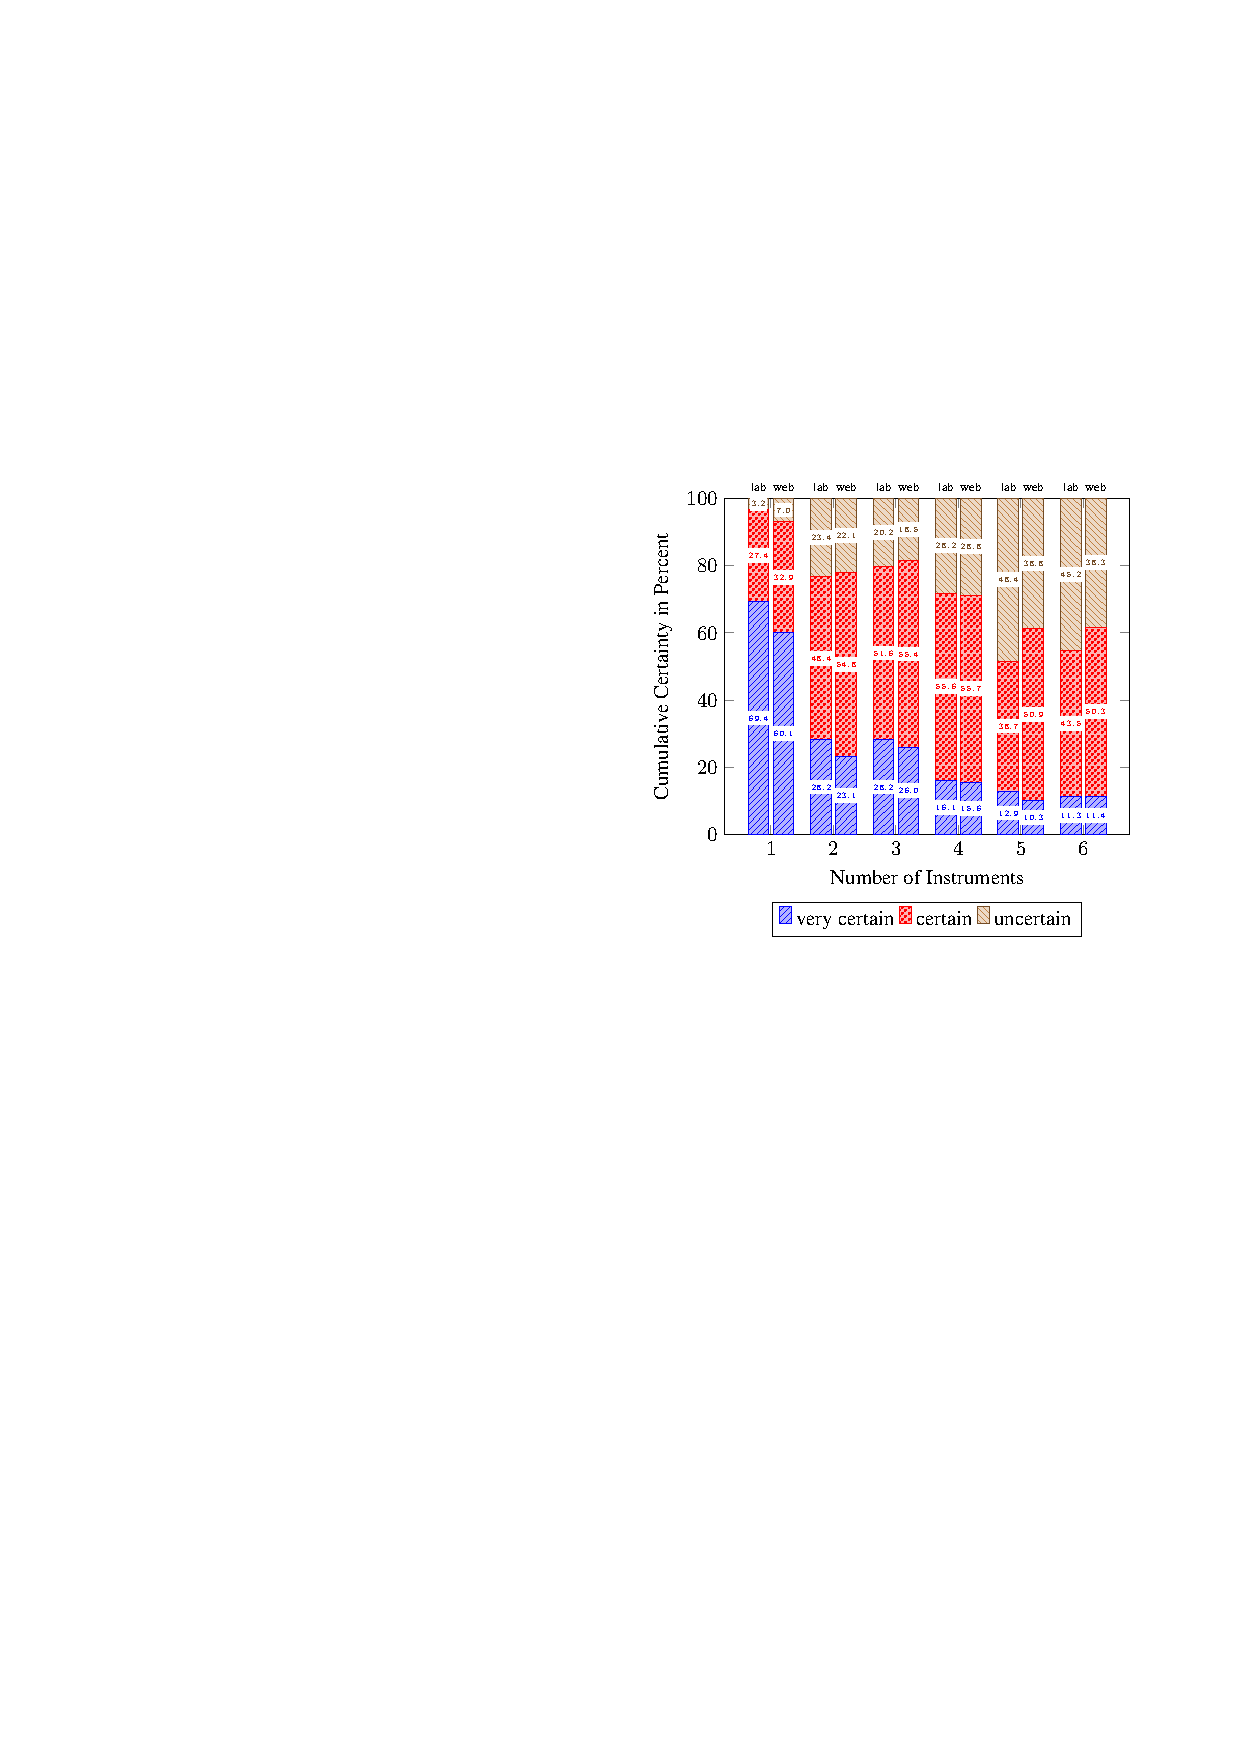
\includegraphics[width=0.45\textwidth]{Chapters/ismir/plotdata/certainty.pdf}
\caption{Differences in certainty between the Internet experiment (web) and laboratory experiment (lab).}
\label{figure:certainty_web_iis}
\end{figure}

To confirm the marginal differences between the Internet experiment and laboratory experiment for $\textit{Dev}_{\mathrm{Abs}}$, a linear regression model was calculated (see Table~\ref{table:lm_absolute_deviation}). Compared to the predictor variable $\textit{Num}_{\mathrm{Inst}}$, the coefficient of $\textit{Environment}$ is very low.
\begin{table}[h]
\center
\scriptsize
\begin{tabular*}{0.45\textwidth}{p{1.5cm}ccccp{0.8cm}}
\toprule[1.5pt]
Coefficient & Estimate & Std. Error & z-value & p-value\\
\midrule
(Intercept) & 0.08535 & 0.02706 & 3.154 & 0.00161\\
$\textit{Num}_{\mathrm{Inst}} = 2$ & 0.17683 & 0.01881 & 9.401  & \textless~2e-16\\
$\textit{Num}_{\mathrm{Inst}} = 3$ & 0.30122 & 0.01881 & 16.014  & \textless~2e-16\\
$\textit{Num}_{\mathrm{Inst}} = 4$ & 1.02154 & 0.01881 & 54.309  & \textless~2e-16\\
$\textit{Num}_{\mathrm{Inst}} = 5$ & 1.67967 & 0.01881 & 89.297  & \textless~2e-16\\
$\textit{Num}_{\mathrm{Inst}} = 6$ & 2.56667 & 0.01881 & 136.453  & \textless~2e-16\\
$\textit{Environment} = \textrm{`}web\textrm{'}$ & 0.05481 & 0.02482 & 2.208  & 0.02724\\
\midrule
\multicolumn{5}{l}{Residual standard error: 0.6597 on 14753 degrees of freedom}\\
\multicolumn{5}{l}{Multiple R-squared: 0.6603,	Adjusted R-squared: 0.6602}\\
\multicolumn{5}{l}{F-statistic:  4779 on 6 and 14753 DF,  p-value: \textless~2.2e-16}\\
\bottomrule[1.5pt]
\end{tabular*}
\caption{Linear regression model for $\textit{Dev}_{\mathrm{Abs}}$ calculated from the data obtained by the Internet experiment and the laboratory experiment.}
\label{table:lm_absolute_deviation}
\end{table}

Another response variable that was obtained from the participants was the certainty of their estimation. Figure~\ref{figure:certainty_web_iis} depicts the certainty values for the Internet experiment and the laboratory experiment.


For testing whether the environment has a significant influence on the certainty of the participants ($\textit{Certainty}$), a cumulative link model (also called ordered regression model) was calculated\cite{Christensen2012}. The cumulative link model is used since $\textit{Certainty}$ is an ordered dependent variable with the possible values `uncertain', `certain' and `very certain'. The predictor variables for the ordered regression model are $\textit{Num}_{\mathrm{Inst}}$ and $\textit{Environment}$. In Table~\ref{table:olr_both} is the cumulative link model for $\textit{Certainty}$ described.
\begin{table}[t]
\center
\scriptsize
\begin{tabular*}{0.45\textwidth}{cccccc}
\toprule[1.5pt]
Coefficient & Estimate & Std. Error & z-value & p-value\\
\midrule
$\textit{Num}_{\mathrm{Inst}} = 2$ & -1.61273 & 0.05744 & -28.078  & \textless~2e-16\\
$\textit{Num}_{\mathrm{Inst}} = 3$ & -1.43164 & 0.05701 & -25.114  & \textless~2e-16\\
$\textit{Num}_{\mathrm{Inst}} = 4$ & -2.02315 & 0.05804 & -34.858  & \textless~2e-16\\
$\textit{Num}_{\mathrm{Inst}} = 5$ & -2.47933 & 0.05901 & -42.013  & \textless~2e-16\\
$\textit{Num}_{\mathrm{Inst}} = 6$ & -2.43573 & 0.05900 & -41.283  & \textless~2e-16\\
$\textit{Environment} = \textrm{`}web\textrm{'}$ & -0.01008 & 0.07355 & -0.137  & 0.891\\
\midrule
\multicolumn{5}{l}{Threshold coefficients:}\\
& Estimate & Std. Error & z-value &\\
$uncertain|certain$ & -2.90465 & 0.08434 & -34.441  &\\
$certain|very certain$ & -0.41072 & 0.08090 & -5.077  &\\
\multicolumn{5}{l}{AIC: 28242.52}\\
\bottomrule[1.5pt]
\end{tabular*}
\caption{Logit cumulative link model of certainty that was calculated from the data obtained by the Internet experiment and the laboratory experiment.}
\label{table:olr_both}
\end{table}
Same as $\textit{Resp}_{\mathrm{Correct}}$, the environment of the experiment has no significant influence on the dependent variable $\textit{Certainty}$. Considering the number of participants and the comparable low coefficient, the environment had a very low influence on $\textit{Certainty}$.

\vspace{-0.1in}
\section{Discussion}\label{sec:discussion}

Regarding the ability of estimating the number of instruments, the web experiment confirmed the results of the laboratory experiment\cite{Stoter2013}. Both experiments share the same outcome: The probability to correctly estimate up to about three instruments is higher than 50\%.

In our previous result analysis of the laboratory experiment\cite{Stoter2013} we set the focus on the differences between musicians and non-musicians. Between the Internet experiment and the laboratory experiment, slightly different results were obtained when looking into how musicians and non-musicians performed (Figure~\ref{figure:error_probability_iis_vs_web}). In the laboratory experiment musicians performed much better compared to non-musicians than in the Internet Experiment. One reason seems to be that in the laboratory experiment 74.2\% of the musicians had also a professional background in audio. In the Internet experiment only 27.5\% of the musicians had a professional background in audio. Since audio professionals more often have to detect hardly audible differences in audio files they are more trained in this field. As mentioned before, being a musician in our context does just mean that the participant plays an instrument without any information about his expert level or the time he or she spends on practicing.

When examining the responses for items with the same number of instruments being played back, noticeable differences between the genres were found. For the stimuli with $\textit{Num}_{\mathrm{Inst}} \le 4$ the mean of $\textit{Resp}_{\mathrm{Correct}}$ was $53.0\%$ and for non-classical items $62.5\%$. Since the experiment was not designed for testing classical versus non-classical items, we cannot make definitive statements about whether humans are better in estimating instruments for a specific music genre. Moreover, we did not address this issue in our result analysis.

One of the main reasons for conducting the experiment was to find out which influence the Internet environment has on the results. All three regression models which included data of both experiments (Table \ref{table:data_both_lm}, \ref{table:lm_absolute_deviation} and \ref{table:olr_both}) revealed that the Internet environment had only very minor effects on the results. Moreover, despite the large number of participants in both experiments, the predictor variable $\textit{Environment}$ was even not significant in two out of three regression models.

It is often recommended to use headphones instead of loudspeakers for Internet experiments. From the relative low average marginal effect of $\textit{Setup}$ (Table~\ref{table:data_web_lm}), it can be derived that the type of the setup had only minor effects on the results of the Internet experiment.

Surprising was the small number of participants who had to be screened. We excluded 27 participants since they gave at least one non-serious response which is about 2.3\% (1195 participants remained after excluding all trials which were not the first ones). Most of these excluded participants responded with either very high numbers (e.~g. 99) or responded with zeros for their estimated number of instruments being played. We assume that especially participants who responded with zero only wanted to get an impression of the experiment.


% The analysis of certainty revealed how difficult the task of estimating the number of instruments is: For up to three instruments the majority of the participants tend to estimate their level on certainty reliably. In more than half of the responses the participants still felt certain or very certain for items of five and six instruments. which gives another indication for the proposed upper limit of three instruments.

\section{Conclusion}\label{sec:conclusion}
The Internet experiment presented in this paper confirmed the results of a previous laboratory experiment that humans are able to correctly estimate up to around three instruments in music. Furthermore significant differences in performance between musicians and non-musicians found out by the previous experiment were confirmed.
The comparison between the results of the Internet experiment and laboratory experiment revealed that only minor differences between both environments exist. Using headphones instead of loudspeaker is often held to be important when conducting listening tests over the Internet. In this experiment the audio setup used had only a minor influence on the results.
According to these results, experiments in the fields of music perception or music information retrieval related to our procedure are well suited for being conducted over the Internet.


\chapter{Methods}

% % Draft version
% % \documentclass[journal, onecolumn, draftcls, 11pt]{IEEEtran}
% % Final
% \documentclass[journal]{IEEEtran}
% \usepackage[utf8]{inputenc}
% \usepackage{amsmath,amssymb,graphicx,romannum}
% \usepackage{tikz}
% \usepackage{url}
% \usepackage{color}
% \usepackage{mathtools}
% \usepackage{cite}
% \usepackage{booktabs}
% \usepackage{lipsum,adjustbox}
% \usepackage{verbatim}
% \usepackage{tikz}
% \usepackage{pgfplots}
% \usepackage{subcaption}
% \usepackage{multirow}
% \usepackage{hyperref}
% \usepackage{flushend}

% \pgfplotsset{compat=1.14}
% \usetikzlibrary{pgfplots.groupplots}
% \usetikzlibrary{chains,scopes,positioning,arrows,fit}
% \usetikzlibrary{arrows, positioning, patterns, calc, decorations.pathmorphing}
% \usetikzlibrary{colorbrewer}
\tikzset{every pin/.style = {font = \small}}
\definecolor{FCNN}{rgb}{0.298039215686275,0.447058823529412,0.690196078431373}
\definecolor{CNN}{rgb}{0.333333333333333,0.658823529411765,0.407843137254902}
\definecolor{FCRNN}{rgb}{0.768627450980392,0.305882352941176,0.32156862745098}
\definecolor{CRNN}{rgb}{0.505882352941176,0.447058823529412,0.698039215686274}
\definecolor{RNN}{rgb}{0.8,0.725490196078431,0.454901960784314}

% \hypersetup{
%     bookmarks=true,         % show bookmarks bar?
%     unicode=false,          % non-Latin characters in Acrobat’s bookmarks
%     pdftoolbar=true,        % show Acrobat’s toolbar?
%     pdfmenubar=true,        % show Acrobat’s menu?
%     pdffitwindow=false,     % window fit to page when opened
%     pdfstartview={FitH},    % fits the width of the page to the window
%     pdftitle={CountNet: Estimating the Number of Concurrent Speakers Using Supervised Learning},    % title
%     pdfauthor={Fabian-Robert Stöter, Soumitro Chakrabarty, Bernd Edler, Emanuël A. P. Habets},     % author
%     pdfsubject={Subject},   % subject of the document
%     pdfcreator={Creator},   % creator of the document
%     pdfproducer={Fabian-Robert Stöter}, % producer of the document
%     pdfkeywords={keyword1, key2, key3}, % list of keywords
%     pdfnewwindow=true,      % links in new PDF window
%     colorlinks=false,       % false: boxed links; true: colored links
%     linkcolor=red,          % color of internal links (change box color with linkbordercolor)
%     citecolor=green,        % color of links to bibliography
%     filecolor=magenta,      % color of file links
%     urlcolor=cyan           % color of external links
% }
% Define Math
\newcommand{\duration}{\ensuremath{d}}
\newcommand{\cardinality}{\ensuremath{k}}

% Define color
\definecolor{myblue}{rgb}{0.2,0.2,0.9}
\newcommand{\chakraso}[1]{{\color{myblue}#1}}

% % Autogenerated, do not edit
\newcommand{\revisiondate}{2018-10-12}
\newcommand{\revision}{134f96f}


% chktex-file 46
% chktex-file 45

% \addtolength{\textfloatsep}{0.9em}
% \setlength{\abovecaptionskip}{0.6em}

% \begin{document}
%
% \title{CountNet: Estimating the Number of Concurrent Speakers Using Supervised Learning}
%
% \author{Fabian-Robert Stöter, Soumitro Chakrabarty, \emph{Student Member, IEEE},\\ Bernd Edler, and Emanuël A. P. Habets, \emph{Senior Member, IEEE}
% \thanks{Copyright~\copyright~2017 IEEE.\@ Personal use of this material is permitted. However, permission to use this material for any other purposes must be obtained from the IEEE by sending a request to pubs-permissions@ieee.org.}%
% \thanks{F. Stöter, S. Chakrabarty, B. Edler and E.A. Habets are with the International Audio Laboratories Erlangen, a joint research institute between the Friedrich-Alexander University Erlangen-Nürnberg (FAU) and Fraunhofer Institute of Integrated Circuits, IIS, Erlangen, Germany (e-mail: fabian-robert.stoeter@audiolabs-erlangen.de)}%
% }
%
% \markboth{{IEEE/ACM} TRANSACTIONS ON AUDIO, SPEECH, AND LANGUAGE PROCESSING, VOL. XX, NO. X, MMM YYYY}%
% {Stöter \MakeLowercase{\textit{et al.}}: CountNet: Estimating the Number of Concurrent Speakers Using Supervised Learning}
%
% \maketitle

\begin{abstract}
Estimating the maximum number of concurrent speakers from single-channel mixtures is a challenging problem and an essential first step to address various audio-based tasks such as blind source separation, speaker diarization, and audio surveillance.
% Building upon powerful machine learning methodology and the possibility to generate large amounts of learning data, Deep Neural Network (DNN) architectures are well suited to directly estimate speaker counts.
We propose a unifying probabilistic paradigm, where deep neural network architectures are used to infer output posterior distributions.
These probabilities are in turn processed to yield discrete point estimates.
Designing such architectures mostly involves two important and complementary aspects that we investigate and discuss.
First, we study how recent advances in deep architectures may be exploited for the task of speaker count estimation.
In particular, we show that convolutional recurrent neural networks clearly outperform recurrent networks used in a previous study when adequate input features are used.
Even for short segments of speech mixtures, we can reliably estimate up to five speakers, with a significantly lower error than other methods.
Second, through comprehensive evaluation, we compare the best-performing method to several baselines, as well as the influence of gain variations, different data sets, and reverberation.
The output of our proposed method is compared to human performance.
Finally, we give insights into the strategy used by our proposed method.
\end{abstract}


% \begin{IEEEkeywords}
% speaker count estimation, number of concurrent speakers, overlapped speech, cocktail-party
% \end{IEEEkeywords}

%!TEX root = ../stoeter_sourcecount.tex
\section{Introduction}%
\label{sec:introduction}
% Introduce the task of estimating the maximum number of concurrent speakers in a single-channel mixture.
% * Lets start right into the task
% Source Separation (count estimate make blind SS fully blind)
In a ``cocktail-party'' scenario, one or more microphones capture the signal from many concurrent speakers. In this setting, different applications may be envisioned such as localization, crowd monitoring, surveillance, speech recognition, speaker separation, etc.
When devising a system for such a task, it is typically assumed that the actual number of concurrent speakers is known.
This assumption turns out to be of paramount importance for the effectiveness of subsequent processing.
Notably, for separation algorithms~\cite{common10},
real world systems do not straightforwardly provide information about the actual number of concurrent speakers.
% Assuming knowledge of speaker counts thus appears more as convenient than as realistic in practice.
It therefore is desirable to close the gap between theory and practice by devising reliable methods to estimate the number of sound sources in realistic environments.
Surprisingly, very few methods exist for this purpose in an audio context, in particular from a single microphone recording.

\par

% TODO: Maybe mention model selection, spectral clustering, gap statistics etc.
%% Transition paragraphs
% Describe two ways of getting the number of speakers: Counting vs Estimation
From a theoretical perspective, estimating the number of concurrent speakers is closely related to the more difficult problem of \textit{identifying} them, which is the topic of speaker diarization~\cite{angueramiro12, rouvier13, rouvier15, ramaiah17}. Intuitively, if a system is able to tell who speaks when, it is naturally also able to tell how many speakers are actually active in a mixture. We call this ``counting by detection''.
As diarization only works when a clear segmentation is possible, the first step of such a strategy often is to find homogeneous segments in the audio where only one speaker is active.
The segment borders can be found by speaker change detection~\cite{Yin17}.
These homogeneous segments are used to discriminate and temporally locate the speakers within a given recording.
When sources are simultaneously active, as in real cocktail party environments, such a segmentation is hardly possible.
In fact, overlapping speech segments typically are a major source of error in speaker diarization~\cite{angueramiro12}.
To improve the robustness of these detection-based methods, a number of approaches attempt to detect and possibly reject the overlapping speech segments to improve performance~\cite{boakye08, huijbregts09, geiger13, andrei17}.
In any case, diarization appears as a very complex problem to tackle when one is only interested in the number of concurrent speakers.
% * Briefly explain differences between counting by detection and directly estimate a count
% with respect to regression or classification. We want to directly estimate the count!
% * Explain how humans count/estimate.
% * Indications that humans are able to do directly estimate vision.
% * How do humans do count and why can't machines?
\par
When speaker overlap is as prevalent as in a ``cocktail-party'' scenario, developing an algorithm to detect the number of speakers is challenging.
This is in contrast to humans where we know that humans are excellent in segregating one source from a mixture~\cite{bregman} and tend to use this skill to perceptually segregate speakers before they can estimate a count, as highlighted, e.g.\ in~\cite{kawashima15}.
As shown in~\cite{kashino96, kawashima15}, humans are able to correctly estimate up to three simultaneously active speakers without using spatial information.
Similarly, in music, psycho-acoustic researchers came up with a ``one-two-three-many'' hypothesis~\cite{huron89, stoeter13, schoeffler13}.
The question if machines could outperform humans, or if they are subject to similar limitations, remains to be answered.
%
\par
Identifying isolated sources in realistic mixtures is challenging~\cite{bregman} and psychology studies in vision~\cite{jevons1871} have shown that humans can instantly estimate the number of objects without actually counting and therefore identifying them.
This phenomenon is known as \textit{subitizing} and has been inspiring research in vision~\cite{chattopadhyay17}.
Since there are indications that the auditory system is also capable of subitizing sources~\cite{hoopen79}, we transfer this fact to the audio domain and directly attempt in this study to estimate the number of audio sources instead of counting them after identification.
We refer to this strategy as ``direct count estimation''.

\par

%% State-of-the-art
% Reference counting methods with restrictions to audio and concurrent speech.
% * Single-channel vs. multi-channel (harder problem is single-channel)
Directly estimating the number of sources in audio mixtures has many applications and appears as a reasonable objective that mimics the process of human perception.
Since humans do have two ears that provide spatial diversity, a first natural idea to imitate human performance is to exploit \textit{binaural} information to proceed to source count estimation.
In terms of signal processing, this is achieved by estimating directions of arrival (DoA) and clustering them~\cite{loesch08, araki09, arberet10, pavlidi12, drude14_icassp, mirzaei15, walter15, Pasha17_reverb}.
However, many audio devices provide only a single microphone signal, and being able to also count sources in that case is desirable. Thus, the single-channel scenario has been considered in many studies:
\par
One of the first methods was proposed 2003 by Arai~\cite{arai03}.
It is based on the assumption that speech mixed from more than one speaker has a more complex amplitude modulation pattern than a single speaker.
The modulation pattern is aggregated and used as a decision function to distinguish between different number of speakers.
In~\cite{sayoud10}, the authors propose an energy feature based on temporally averaged mel filter outputs.
The number of concurrent speakers was determined by manually determining thresholds that best match individual speaker counts.
In a more recent work,
Xu et.al.~\cite{xu13} estimate the number of speakers by applying hierarchical clustering on fixed-length audio segments using mel frequency cepstral coefficients (MFCCs) and additional pitch features.
The method assumes non-overlapped speech and was evaluated on real world data of 20 hours duration and an average count estimation error of one speaker is reported using excerpts of eight-minutes duration and featuring up to eight speakers.
In another vein, Andrei et.al.~\cite{andrei15_interspeech} proposed an algorithm which correlates single frames of multi-speaker mixtures with a set of single-speaker utterances.
The resulting score was then used to estimate the number of speakers using thresholds.

\par

%% What is the gap?
In all the aforementioned methods, the speaker count estimation problem was devised.
The different strategies undertaken there rely on classical and grounded signal processing strategies and exhibit fair performance in a controlled setup.
However, our experience shows (see Section~\ref{sec:evaluation}) that they leave much room for improvement when applied to more diverse and challenging signals than those corresponding to their targeted applications, notably in the case of many different and constantly overlapping speakers.
% * Existing single-channel methods require segments where only a single speaker is active.
This is due to their main common weakness, which is to rely on the assumption that there are segments where only one speaker is active, in a way that is similar to the classical speaker diarization studies mentioned before.
In~\cite{stoeter17} a first data-driven approach based on a recurrent network was presented, motivated by the recent and impressive successes of deep learning approaches in various audio tasks like speech separation~\cite{yu16, hershey16, grais17} and speaker diarization~\cite{yella14, hruz16, garciaromero17}.
The methods proposed in~\cite{stoeter17} to address speaker count estimation using deep learning were built upon recent methods to count objects in images, which is a popular application with many contributions from the deep learning community~\cite{wang15, chattopadhyay17, khan16, segui15, zhang15, arteta16, marsden16, boominathan16, zhang2015salient}.
In~\cite{stoeter17} two main paradigms were evaluated: a) count estimation as regression problem, where the systems are directly trained to output the number of objects as a point estimate, and b) classification, where every possible number of objects is encoded as a different class and the output of a predicting system corresponds to a probability distribution over these classes.
The results of the proposed method indicated that a classification based neural network performed better than one based on regression.
One drawback however is that the maximum number of speakers (the number of classes) is known in advance.

% Many tasks in machine learning are formulated as classification problems and many models were proposed to address count estimation in this setup~\cite{segui15, zhang2015salient, khan16}, with good performance.

\par

In this study, we build upon~\cite{stoeter17} and focus on the network architecture design, as well as on finding limitations for different test scenarios.
This work makes the following contributions:
%% List of Contributions
% * Defining the problem of Estimating Number of Concurrent Sources.
i) we generalize the problem formulation by fusing classification and regression, which allows to estimate discrete outputs while controlling the error term. This is done by picking a point estimate from a full posterior distribution provided by the deep architectures;
% * Influence of three different problem formulations: regression, poisson regression. classification
% * Solution: Investigation of several deep learning architectures.
ii) in addition to the recurrent network introduced in~\cite{stoeter17}, we propose alternative speaker-independent neural network architectures based on the convolution operation to improve count estimation.
Each of the proposed networks is adjusted to estimate the number of speakers from audio segments shorter than 10 seconds;
iii) we test the performance of these networks in multiple experiments and compare them to several baseline methods, pointing out possible limitations.
Furthermore, we present a statistical analysis of the results to determine whether classification outperforms regression for all architectures;
% * Experiments aim to identify the learned strategy.
iv) we conducted a listening experiment to relate the best-performing machine to human performance.
We describe one of the strategies taken by the data-driven approach that might explain its superior performance.
Finally, for the sake of reproducibility, the trained networks (models) as well as the test dataset are made available on the accompanying website\footnote{\url{https://www.audiolabs-erlangen.de/resources/2017-CountNet}.}.
\par
%% Organisation
The remainder of this paper is organized as follows. In Section~\ref{sec:problem_formulation}, we describe the count estimation problem formally and the general ideas we propose to tackle it.
In Section~\ref{sec:supervised_learning}, we propose several architectures, each of them adjusted to estimate the number of speakers from short audio segments of less than 10~s.
In Section~\ref{sec:hyperparameters}, we then assess several common hyper parameters for all of our proposed architectures, so that we are able to propose a single, best performing model.
In Section~\ref{sec:evaluation} this model is compared to several baseline systems under various acoustical conditions.
Additionally, we compare the proposed method to human performance.
We point out possible limitations and provide indications for the strategy being taken by the DNN in Section~\ref{sec:ablation} before we conclude in Section~\ref{sec:conclusion}.

%!TEX root = ../stoeter_sourcecount.tex
% chktex-file 46
% chktex-file 45

\section{Problem Formulation}%
\label{sec:problem_formulation}
% introduce the section
We consider the task of estimating the maximum number of concurrent speakers \( \cardinality \in \mathbb{Z}^{+}_{0} \) in a single-channel audio mixture \(\mathbf{x}\).
This is achieved by applying a mapping from \(\mathbf{x}\) to \(\cardinality \).
We now provide details on the notations, the general structure of the method, and various ways to exploit the deep learning framework to estimate \(\cardinality \).

\subsection{Signal Model}%
\label{ssec:signal_model}
Let \(\mathbf{x}\) be a vector with \(N\) discrete time samples, representing a linear mixture of \(L\) single speaker speech signal vectors \(\mathbf{s}_l\).
The value observed at sample~\(n\) for the mixture is given by~$x_n$ and for the individual speech segments by~$s_{nl}$.
The mixture then results in
%
\begin{equation}
  x_n = \sum_{l=1}^{L}{s_{nl}} \; \forall n \in \mathbb{Z}^N.
  \label{eq:mixing_model}
\end{equation}
%
Naturally, each speaker~$l=1,\dots,L$ is not active at every time instant.
On the contrary, we assume there is a latent binary \textit{speech activity} variable~$v_{nl}\in \left\{ 0,1 \right\}$ that is defined as:
\begin{equation}
v_{nl}=\begin{cases}
1 & \text{if }\left|s_{nl}\right|>0\\
0 & \text{otherwise}.
\end{cases}\label{eq:definition_speech_activity}
\end{equation}

Our objective of estimating the maximum number of concurrent speakers can now be formulated as
%
\begin{equation}
k=\underset{n}{\max}\left(\sum_{l = 1}^{L} v_{nl}\right) \; n \in \{ 1,\ldots, N \}
\label{eq:definition_k}.
\end{equation}
%
As can be seen, our proposed task of estimating $k\leq L$, is more closely related to source separation whereas the estimation of \(L\) is more useful for tasks where speakers do not overlap.
For instance, three non-overlapping speakers would result in \(L = 3\) and \(\cardinality = 1\).
In the rest of this work, we assume that no additional prior information about the speakers is given to the system except possibly the maximum number of concurrent speakers~$k_{\max}$, that is application-dependent and represents an upper bound for the estimation.

While speaker diarization would mean estimating the whole speech activity matrix~$v_{nl}$ in~(\ref{eq:definition_speech_activity}), our problem of estimating only~$k$ in~(\ref{eq:definition_k}) is more abstract as it requires a direct estimation of the count as advocated in Section~\ref{sec:introduction}.
\begin{figure}[t]
  \centering
  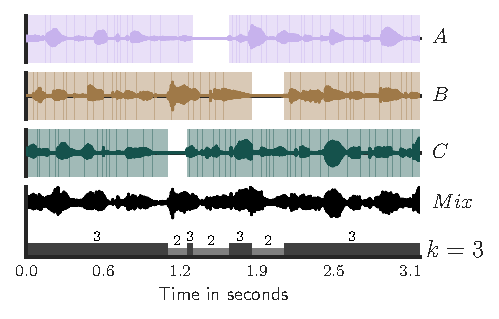
\includegraphics[width=0.8\columnwidth]{Chapters/dsc/figures/teaser.pdf}
  \caption{Illustration of our application scenario of three concurrent speakers (A, B, C) and their respective speech activity. Bottom plot shows the mixture (input), the number of concurrently active speakers and its maximum \(k\) which is our targeted output.}%
  \label{fig:teaser}%
\end{figure}
In Figure~\ref{fig:teaser}, we illustrate our setup in a ``cocktail-party'' scenario featuring~$L=3$ unique speakers.
At any given time, we see that at most~$k=L=3$ speakers are active at the same time and~$k=2$ could be the outcome if a smaller excerpt would be evaluated.

Now, the system we propose is actually not inputting the signal vector $\mathbf{x}$, but rather a Time-Frequency (TF) representation as the absolute value of the Short-Term Fourier Transform of~$\mathbf{x}$ that is denoted by $\mathbf{X}$.
In the following, $\mathbf{X}$ is the non-negative input for the system.

\subsection{Probabilistic formulation}%
\label{ssec:model}
In a supervised scenario, let~$ \left\{\mathbf{X}_t,k_t\right\}_t$ be all of our learning examples, where~$t \in{1,\dots,T}$ denotes the $t$-th training item from the training database.
For the purpose of learning a mapping between~$\mathbf{X}$ and~$k$, we adopt a probabilistic viewpoint and introduce a flexible generative model that explains how a particular source count~$k$ corresponds to some given input ~$\mathbf{X}$.

First, we consider that all training samples~$\left\{\mathbf{X}_t,k_t\right\}_t$ are independent.
For each sample, we consider that~$k_t$ is drawn from a probability distribution of a known parametric family, parameterized by some latent and unobserved parameters~$\mathbf{y}_t$
\begin{equation}
\mathbb{P}\left(k_{t}\mid\mathbf{X}_{t}\right)=\mathcal{L}\left(k_{t}\mid \mathbf{y}_{t}\right),
\end{equation}

% @soumitro
% \begin{equation}
% k_{t} \sim \mathcal{P}(k_{t} | \mathbf{y}_{t})
% \end{equation}

the distribution~$\mathcal{L}\left(\cdot\mid \mathbf{y}_{t}\right)$ is called the \textit{output distribution} in the following.
We further assume that there is some deterministic mapping between~$\mathbf{X}_t$ and~$\mathbf{y}_t$, embodied as
\begin{equation}
\mathbf{y}_{t}=f_{\mathbf{\theta}}\left(\mathbf{X}_{t}\right),
\end{equation}
where $\mathbf{\theta}$ are the parameters for this deterministic mapping, that is independent of~$t$. This results in an output distribution given by
\begin{equation}
\mathbb{P}\left(k_{t}\mid\mathbf{X}_{t}\right)=\mathcal{L}\left(k_{t}\mid f_{\mathbf{\theta}}\left(\mathbf{X}_{t}\right)\right).\label{eq:output_distribution}
\end{equation}
Assume for the rest of this section that these parameters~$\mathbf{\theta}$ are known.
Given a previously unseen input~$\mathbf{X}$, expression~(\ref{eq:output_distribution}) means we can compute the distribution of the source count~$k$.
% The advantage of that probabilistic formulation is to introduce some flexibility instead of enforcing a more classical deterministic mapping such as~$k_{t}=f_{\mathbf{\theta}}\left(\mathbf{X}_{t}\right)$.

The objective of our counting system is to produce a point estimate~$\hat{k}$ rather than a whole output distribution~$\mathbb{P}\left(k\mid\mathbf{X}\right)$.
A first option is to pick as an estimate the most likely outcome for the output distribution, thus resorting to Maximum A Posteriori (MAP) estimation:
\begin{equation}
\hat{k}=\underset{k}{\text{argmax}}\ \mathcal{L}\left(k\mid f_{\mathbf{\theta}}\left(\mathbf{X}\right)\right).
\end{equation}

However, MAP is not the only option and a broad range of point estimation techniques may be obtained when resorting to decision theory~\cite{berger1985}.
We may for example also choose~$\hat{k}$ as the value that minimizes the marginal average cost of choosing an estimate $\hat{k}$ instead of the true value $k$, when $k$ is distributed with respect to the output distribution
\begin{equation}
\hat{k}=\underset{u}{\text{argmin}}\intop_{k}d\left(k,u\right)\mathcal{L}\left(k\mid f_{\mathbf{\theta}}\left(\boldsymbol{X}\right)\right) \mathrm{d} k,\label{eq:estimate_hatk}
\end{equation}
where $d\left(k,u\right)$ is the cost of picking $u$ as an estimate when the true value is~$k$.
It may be any function that seems appropriate, not restricted to the subject of differentiability.
% For instance, when we take~$d\left(k,u\right)=\left|k-u\right|^{2}$, we obtain the Minimum Mean Squared Error (MMSE) estimate.
However, we retain the more general formulation~(\ref{eq:estimate_hatk}) because other choices will sometimes prove more effective, as we show later.
For notational convenience, we write~(\ref{eq:estimate_hatk}) as
\begin{equation}
\hat{k}=q\left(f_{\mathbf{\theta}}\left(\boldsymbol{X}\right)\right),
\end{equation}
and $q\left(\cdot\right)$ is called the~\textit{decision function}.
Using this strategy, we have everything to produce a single source count estimate~$\hat{k}$ from input features~$\mathbf{X}$, provided the parametric family~$\mathcal{L}$ and the mapping $f_{\mathbf{\theta}}$ as well as its parameters $\mathbf{\theta}$ are known.

In this study, we choose a deep neural network for the mapping $f_{\mathbf{\theta}}$, whose weights~$\mathbf{\theta}$ are trained in a supervised manner.
Once a particular network architecture has been chosen, learning its parameters is achieved through classical stochastic gradient descent.
If we assume that the particular family~$\mathcal{L}$ of output distributions has been chosen, it appears natural to learn the parameters~$\mathbf{\theta}$ that maximize the likelihood of the learning data.
More specifically, the total cost to be minimized becomes
\begin{equation}
C=\sum_{t=1}^{T}-\log\mathcal{L}\left(k_{t}\mid f_{\theta}\left(\boldsymbol{X}_{t}\right)\right).\label{eq:total_cost}
\end{equation}
The derivative of this cost (\ref{eq:total_cost}) with respect to the parameters can be used to learn the network parameters.
\par
Three different choices for the family of output distributions (classification, Gaussian regression and Poisson regression) as well as the corresponding decision functions~$q\left(\cdot\right)$ were investigated and discussed in~\cite{stoeter17}, and the reader is referred to it for further details.


% \subsubsection{Classification}
%
% In a classification setting, the output distribution is directly taken as \textit{discrete}, discarding any meaning concerning the ordering of the different possible values.
% In other words, \(\cardinality \) may only take a finite set of values, whose actual labelling is not assumed to bear any particular information.
% In that case, the output distribution~$\mathcal{L}\left(k\mid f_\mathbf{\theta}\left(\mathbf{X}\right)\right)$ is taken as multinomial with~$L+1$ (when we assume that \(k\) can be 0) classes.
% Given some particular input~$\mathbf{X}$, the network generates the posterior output probability for each of those \((L + 1)\) classes, and a MAP decision function may for instance be chosen that simply picks the most likely class:
%
% \begin{equation}
% \hat{k}=q\left(f_{\mathbf{\theta}}\left(\mathbf{X}\right)\right)=\arg\max\mathcal{L}(k\mid f_{\mathbf{\theta}}\left(\mathbf{X}\right)).
% \end{equation}
%
% Notwithstanding its conceptual simplicity, classification has two drawbacks.
% First, the intuitive ranking between different estimates is lost: e.g. \(p(\cardinality = 6) \) may not depend on \(p(\cardinality = 5) \).
% Second, the largest possible count $L$ is given \textit{a priori}.
% Despite these limitations, classification based approaches have successfully been applied in deep neural networks for counting objects~\cite{segui15, zhang2015salient, khan16} in images.
%
% \subsubsection{Gaussian Regression}
% Compared to classification, where the ordering of $k\in\mathbb{N}$ is not at all taken into account, adopting a strategy where~$k$ derives from an output distribution defined on the real line seems like a desirable setup.
% However, this strategy comes with the additional difficulty of handling the fact that~$k$ is integer.
% To circumvent it, we take $k$ as the rounding of a latent variable $f_{\mathbf{\theta}}\left(\mathbf{X}\right)\in\mathbb{R}$, and exploit the fact that rounding may be efficiently modelled as introducing white additive Gaussian noise, so that we may write:
% \begin{equation}
% k\sim\mathcal{N}\left(f_{\mathbf{\mathbf{\theta}}}\left(\mathbf{X}\right),\Delta\right),\label{eq:AWGN_model}
% \end{equation}
% where $\mathcal{N}$ is the Gaussian scalar distribution and $\Delta$ is the rounding noise variance, that is independent of any model parameters but only depends on the fact that $k$ is the integer closest to $f_{\mathbf{\mathbf{\theta}}}\left(\mathbf{X}\right)$.
%
% As can be seen, the output distribution in that setting becomes the Gaussian and the associated cost function is the classical squared error.
% During inference and given the output~$f_{\mathbf{\mathbf{\theta}}}\left(\mathbf{X}\right)$ of the network, the best discrete value that is consistent with the model is simply the rounding operator $\left[\cdot\right]$:
%
% \begin{equation}
% \hat{k}=\left[f_{\mathbf{\mathbf{\theta}}}\left(\mathbf{X}\right)\right].
% \end{equation}
%
% Gaussian regression has achieved state-of-the-art counting performance in computer vision using deep learning frameworks~\cite{zhang15, arteta16, marsden16, boominathan16}.
%
% \subsubsection{Discrete Poisson modelling}
% When it comes to modelling count data, it is often shown effective to adopt the Poisson distribution.
% First, this strategy retains the advantage of the classification approach to directly pick a probabilistic model over the actual discrete observations, avoiding the somewhat artificial trick of introducing a latent variable that would be rounded to yield the observation.
% Second, that model retains the algebraic structure of $k\in\mathbb{N}$ and thus avoids the inconvenient of the classification approach to completely drop dependencies between classes.
%
% Due to these advantages, the Poisson distribution already enjoyed some use in studies devising deep architectures for counting systems~\cite{Rezatofigh16}.
% In~\cite{fallah09, chan09, Rezatofigh16} it is for instance shown that the number of objects in images can be well modelled by the Poisson distribution. Inspired by these previous work, we also consider the Poisson output distribution:
% \begin{equation}
% \mathbb{P}\left(k\mid f_{\mathbf{\theta}}\left(\mathbf{X}\right)\right)=\mathcal{P}\left(k\mid f_{\mathbf{\mathbf{\theta}}}\left(\mathbf{X}\right)\right),
% \end{equation}
% where $\mathcal{P}\left(\cdot\mid\lambda\right)$ denotes the Poisson distribution with scale parameter~$\lambda$.
%
% In that setup, the cost function at learning time is the Poisson negative log-likelihood and the deep architecture at test time provides the predicted scale parameter $f_{\mathbf{\mathbf{\theta}}}\left(\mathbf{X}\right)\in\mathbb{R}_+$, which summarizes the whole output distribution.
%
% As a decision function~$q$ in that setting, we considered several alternatives. A first option is to again resort to MAP estimation and pick the mode $\left[f_{\mathbf{\mathbf{\theta}}}\left(\mathbf{X}\right)\right]$ of that distribution as a point estimate. However, experience showed that this is not the best choice. After some investigations, it appeared that the posterior median (corresponding to the absolute error $d\left(k,u\right)=\left|k-u\right|$ in~\ref{eq:estimate_hatk}) does yield a better estimation:
% \begin{subequations}
% \begin{align}
% q\left(f_{\mathbf{\mathbf{\theta}}}\left(\mathbf{X}\right)\right) & =\underset{\hat{k}}{\text{argmin}}\sum_{k=0}^{\infty}\left|\hat{k}-k\right|\mathcal{P}\left(k\mid f_{\mathbf{\mathbf{\theta}}}\left(\mathbf{X}\right)\right)\\
%  & =\text{median}\left(k\sim\mathcal{P}\left(f_{\mathbf{\mathbf{\theta}}}\left(\mathbf{X}\right)\right)\right)\\
%  & \approx\left\lfloor f_{\mathbf{\mathbf{\theta}}}\left(\mathbf{X}\right)+\frac{1}{3}-\frac{0.02}{f_{\mathbf{\mathbf{\theta}}}\left(\mathbf{X}\right)}\right\rfloor, \label{eq:decision_function_poisson}
% \end{align}
% \end{subequations}
% where the last expression is a good approximation of the median of a Poisson distributed random variable of scale parameter~$f_{\mathbf{\mathbf{\theta}}}\left(\mathbf{X}\right)$~\cite{Choi94}.

% \begin{figure}[t]
%   \centering
%   \begin{adjustbox}{width=1\columnwidth}
%     \begin{tikzpicture}[>=stealth, auto, node distance=4cm]
    \tikzstyle{every path}=[line width=0.4mm]
    % Place nodes
    % Define the style for the blue dotted boxes
    \tikzset{blue dotted/.style={draw=blue!80!white, line width=1pt,
                          dash pattern=on 1pt off 1pt on 1pt off 1pt,
                           inner sep=4mm, rectangle, rounded corners}};
    \tikzset{red dotted/.style={draw=red!80!white, line width=1pt,
                           dash pattern=on 1pt off 1pt on 1pt off 1pt,
                           rectangle}};
    \tikzstyle{red text}=[text=red!80]
    \tikzstyle{blue text}=[text=blue!80]
    \tikzstyle{block} = [draw, rectangle, inner sep=3pt, minimum width=3cm, minimum height=1cm, align=center]
    \tikzstyle{pinstyle} = [pin edge={to-,thin,blue!80}]
    \tikzstyle{pinstyle2} = [pin edge={-to,thin,red!80, dash pattern=on 1pt off 1pt on 1pt off 1pt}]


    \node [block] (feat) {Feature Extraction};
    \node [block, right of=feat, node distance=4cm] (norm) {Normalisation +\\Standardization};
    \node [block, right of=norm, pin={
      [pinstyle, blue text, name=k_train]above:$k$
    }] (dnn) {DNN};
    \node [block, red dotted, red text, below of=dnn, pin={[pinstyle2, red text, name=k_inf]right:$\hat{k}$}, node distance=2cm] (inference) {q};
    \coordinate [left of=feat, node distance=2cm] (input) {};
    \node at ($(k_train.east)+(11mm, 0)$) [blue text, above, inner sep=3mm] {\textbf{Training}};
    \node at ($(inference.south east)+(0, -3mm)$) [red text, below, inner sep=3mm] {\textbf{Inference}};

    % Connect nodes
    \draw [->] (input) -- node {$x$} (feat);
    \draw [->] (feat) -- node {$\mathbf{X}$} (norm);
    \draw [->] (norm) -- (dnn);
    \draw [dash pattern=on 1pt off 1pt on 1pt off 1pt, ->] (dnn) -- node {$y$} (inference);

\end{tikzpicture}

%   \end{adjustbox}
% \caption{%
% Block diagram of the proposes supervised learning model.
% Training is realised using tuples of spectro-temporal inputs \(\mathbf{X}\) and
% the true number of concurrent speakers \(k\). For inference the output \(y\) is post-processed using a decision function \(q\) to generate estimates \(\hat{k}\).
% }%
% \label{fig:blockdiagram}
% \end{figure}

%!TEX root = ../stoeter_sourcecount.tex
\section{DNNs for Count Estimation}%
\label{sec:supervised_learning}
% A short review of deep learning architectures used for related tasks and proposal for count estimate architectures.
Applying deep learning to an existing task, often is a matter of choosing a suitable network architecture.
Typically an architecture describes the overall structure of the network including (but not limited to) the type and number of layers in the network and how these layers are connected to each other.
In turn, designing such an architecture requires deep knowledge about input and output representations and their required level of abstraction.
% Introduce our three/five basic networks. For all of them we:
% * reference the use cases, and the strengths and weaknesses,
% * explain why and how they can be used for count estimation
Many audio related applications like speech recognition~\cite{HintonSpeech} or speaker diarization share similar common architectural structures, often found by incorporating domain knowledge and through extensive hyper parameter searches.
For our task of source count estimation, however, domain knowledge is difficult to incorporate, as our studies aim at revealing the best strategy to address the problem.
This is why we chose architectures that already have shown a good level of generalizability for audio applications.
All architectures under investigation are summarized in Figure~\ref{fig:networkoverview}.
\par
% introduce some basic notations for the input
The input of all networks is a batch of samples, represented as time frequency representations \(\mathbf{X} \in \mathbb{R}^{ D \times F \times C } \), where \(D\) refers to the time dimension, \(F\) to the frequency dimension and \(C\) to the channel dimension (in the single-channel case, \(C=1\)).
In the following, we discuss several commonly used DNN architectures and their benefits in using them for the task of estimating the number of speakers.


\subsubsection{Convolutional Neural Network (CNN)}%
Convolutional Neural Networks (CNNs) are a variant of standard fully-connected neural networks, where the architecture generally consists of one or more ``convolution layers'' followed by fully-connected layers leading to the output.

A convolution layer generally consists of a convolution operation, followed by feature pooling.
The convolution operation applies a set of filters to local regions of the input, and the application of each such filter outputs a \emph{feature map}.
It should be noted that the convolution operation, generally, also constitutes the application of a point-wise non-linear activation function on each feature map.
This is followed by feature pooling, that aims to reduce the feature space dimensions by combining the filter activations over a specified region.
Since the individual elements of the filters (weights) are learned during the training stage, convolution layers can also be interpreted as feature extractors.
By stacking up additional layers, CNNs can extract more abstract features in higher level layers~\cite{Simonyan15}.
\par
The sizes of the filter kernels are crucial, and it was shown in~\cite{pons2017timbre} that many audio applications can benefit if domain knowledge is put into the design of the filter kernel size.
The use of small filter kernels, as often used in image classification tasks, does not necessarily decrease performance, when combined with many layers.
Also larger kernels increase the number of parameters and therefore the computational complexity.
It was shown in~\cite{schluter15} that \(3 \times 3\) kernels resulted in state-of-the-art results in singing voice detection tasks.
Due to its hierarchical architecture, CNNs with small filters have the benefit that they can model time and frequency invariances regardless of the scaling of the frequency axis.
\par
Our proposed architecture is similar to the ones proposed by ~\cite{schluter16} used for singing voice activity detection.
In our proposed CNN, we consider local filters of size \(3 \times 3\). In the first layer, 2D convolution is performed by moving the filter across both dimensions of the input in steps of 1 element (striding \(s = 1\) to generate \(C = 64\) feature maps/channels resulting in an output volume of \(64 \times (D - 3 + 1) \times (F - 3 + 1)\).
In the subsequent convolution layers, a similar operation is applied but for each convolutional layer, we consider a different number of feature maps.
Note, that the convolution operation is performed independently for every input channel, and then summed up along the dimension \(C\) for each output element.
In preliminary experiments we found that by using max-pooling we received significantly better performance when used after CNN layers.

\subsubsection{Recurrent Neural Network (RNN)}%
While convolutional layers excel in capturing local structures, RNNs can detect structure in sequential data of arbitrary length.
This makes it ideal to model time series, however, in practice, the learned temporal context is limited to only a few time instances, because of the vanishing gradient problem~\cite{Hochreiter98}.
To alleviate this problem, forgetting factors (also called gating) were proposed.
One of the most popular variants of RNNs with forgetting factors is the Long Short-Term Memory (LSTM)~\cite{Hochreiter97} cell.
In~\cite{stoeter17} such an architecture based on three bi-directional LSTM cells, was proposed. The architecture is similar to the one employed in~\cite{Leglaive15}.

% \begin{figure}[t]
% \centering
% 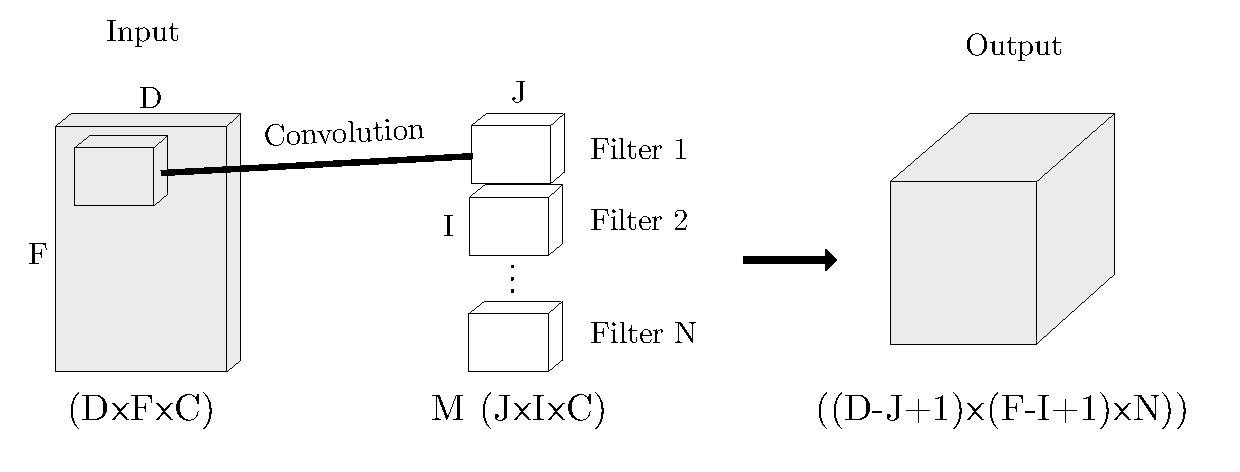
\includegraphics[width=\columnwidth]{figures/conv.pdf}
% \caption{Illustrative diagram to show the convolution operation in
% convolution layers of CNN.\@ We consider N different local filters each
% of size \(J\times I\)}%
% \label{fig:conv}
% \end{figure}

% * good for temporal dependencies.
% * State-of-the-art speech recognition, NLP, diarization
% A recurrent neural network (RNN) layer is very similar to a fully connected network, except that RNN applies the same set of weights \(\mathbf{A}\) recursively over an input sequence.
% While convolutional layers excel in capturing local structures, RNNs can detect structure in sequential data of arbitrary length. %have an internal memory of infinite length of the past input sequence history.
% This makes it ideal to model time series, however, in practice, the temporal context learnt is limited to only a few time instances, because of the vanishing gradient problem~\cite{Hochreiter98}.
%
% To alleviate this problem, forgetting factors (also called gating) were proposed.
% One of the most popular gated recurrent cells is the Long Short-Term Memory (LSTM)~\cite{Hochreiter97} cell.
% Its effectiveness has been proven in various applications and LSTMs are the state-of-the-art approach for speech recognition~\cite{Graves13} and singing voice detection~\cite{Leglaive15}~\footnote{For a deeper mathematical background of LSTMs, due to space constraints, the reader is referred to the aforementioned papers.}.
% For a given input of dimensions \(D \times F \times C\), the output of a recurrent layer is either only the last step of dimension \(1 \times A\) or the full sequence \(D \times A\).
% The latter is useful to stack multiple LSTMs or to apply temporal max pooling of the sequence.

\subsubsection{Convolutional Recurrent Neural Network (CRNN)}%
% * Combination of CNN and Recurrent
Recently the a combination of convolutional and recurrent (LSTM) layers were proposed for audio related tasks~\cite{sainath15, amodei16, Choi17, cakir17}.

The main motivation to stack these layers is to combine the benefits of convolutional layers with those of recurrent architectures, namely the benefit of convolutional layers in aggregating local features with the ability of recurrent layers to model long-term temporal data.

There are different ways to stack CNNs and RNNs to form a CRNN architecture.
In our application the motivation is to aggregate local time-frequency features coming from the output convolutional neural network and use the LSTM layer to model long temporal structures.
As the output of a CNN layer is a 3D volume \(D \times F \times C\) and the input of a recurrent layer only takes a 2D sequence, the dimension would need to be reduced. Naturally, the time dimension would need to be kept, therefore the channel dimension \(C\) is stacked with the frequency dimension \(F\) resulting in a \(D \times F \cdot C\) output.
% \begin{figure}[t]
% \centering
% 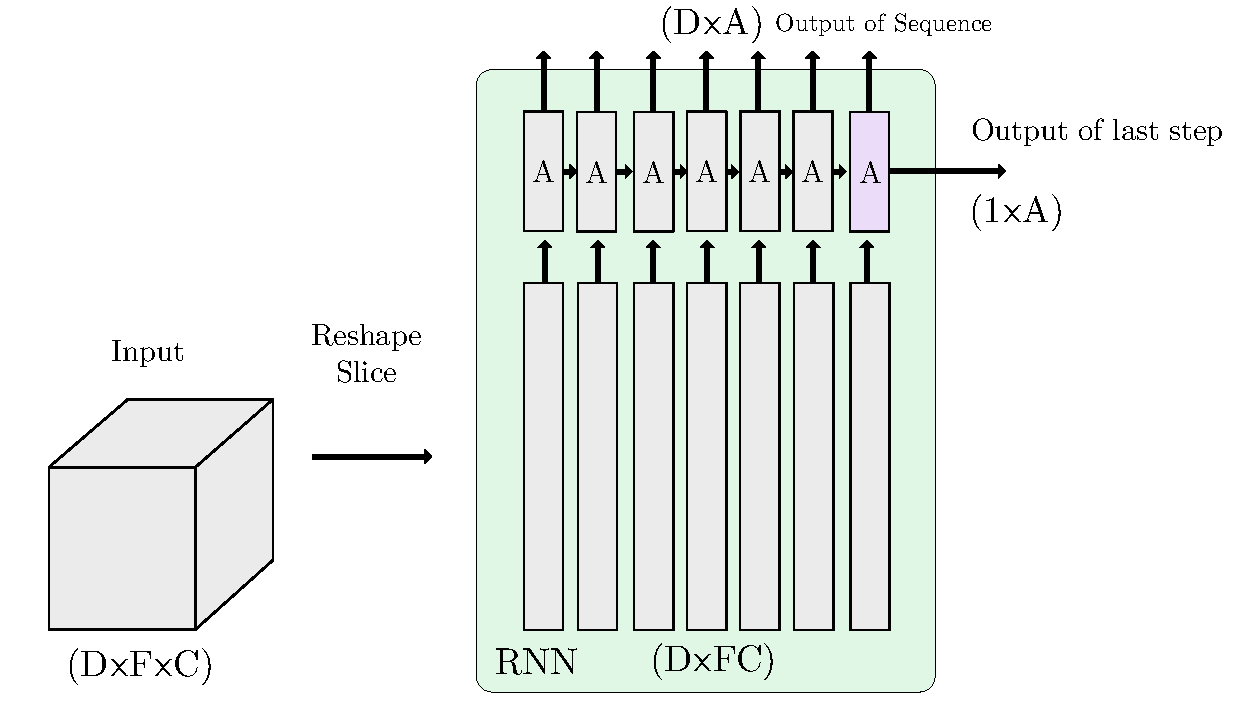
\includegraphics[width=\columnwidth]{figures/crnn.pdf}
% \caption{Illustrative diagram to show the stacking of the output of a convolution layer into a recurrent layer with \(A\) hidden nodes per memory cell.}%
% \label{fig:crnn}
% \end{figure}

\subsubsection{Full-band Convolutional Neural Networks (F-CNN)}%
% * using full frequency band filters.
% * Very few Parameters, easy to train.
Architectures where filters span the full frequency range and therefore apply convolution in temporal direction only, have already been successfully deployed in speech~\cite{amodei16} and music application~\cite{Choi17, Pons16, Dieleman14}).
Our motivation here is that the activity of speakers happen over wide frequency ranges and a count (unlike in counting objects in images) cannot be split into sub counts.
The full-range kernel configuration only affects the first hidden layer, as in consecutive outputs all frequency bands are squashed down to one single frequency band using ``valid'' convolutions.
This is computationally very efficient, because it reduces the middle layer's dimensionality of the network significantly due to this aggregation.
To further optimize the performance of the network, we applied a hyper parameter optimization technique using Tree-structured Parzen Estimator (TPE)~\cite{bergstra11}.
We used a search space of several hyper parameters as shown in Table~\ref{tab:fcnnhyper} and set the maximum number of evaluations to 200.

\begin{table}
  \caption{Parameter Optimization of F-CNN Model through hyper-parameter search. Bold hyper-parameters were found optimal.}%
  \label{tab:fcnnhyper}
  \centering
\begin{tabular}{lll}
  \toprule
  Layer               & Parameters        & Value Range \\
  CNN 1               & Feature Maps      & \( \{16, \mathbf{32}, 64\} \) \\
  CNN 1               & Filter Length     & \( \{\mathbf{3}, 5, 7\} \) \\
  Pooling 1           & Pooling Length    & \( \{1, \mathbf{2}, 4\} \) \\
  CNN2                & Feature Maps      & \( \{16, \mathbf{32}, 64\} \) \\
  CNN2                & Filter Length     & \( \{\mathbf{3}, 5, 7\} \) \\
  Pooling 2           & Pooling Length    & \( \{1, 2, 4\} \) \\
  \midrule
  CNN 3               & Presence of Layer & \( \{\mathbf{Yes}, No\} \) \\
  CNN 3               & Feature Maps      & \( \{16, 32, \mathbf{64}, 128\} \) \\
  CNN 3               & Filter Length     & \( \{\mathbf{3}, 5, 7\} \) \\
  Pooling 3           & Pooling Length    & \( \{1, \mathbf{2}, 4\} \) \\
  \midrule
  Fully Connected 1   & Hidden Unit       & \( \{64, \mathbf{128}\} \) \\
  Dropout 1           & Dropout Percentage& \( [0.1, \mathbf{0.2}, 0.5] \) \\
  Fully Connected 2   & Hidden Unit       & \( \{32, \mathbf{48}\} \) \\
  Dropout 2           & Dropout Percentage& \( [0.1, \mathbf{0.2}, 0.5] \) \\
  \bottomrule
  \end{tabular}
\end{table}

The results are in agreement with the findings in~\cite{schluter16} where small filter kernels of size 3 outperformed larger kernels. Also it can be seen from the results, that increasing the number of feature maps of the convolutional layers does not necessarily increase the performance.

\subsubsection{Full-Range Convolutional Recurrent Neural Networks (F-CRNN)}%
% * Also add recurrent.
Similarly to \emph{CRNN} and to the Deep Speech 2 implementation~\cite{amodei16}, we added an LSTM recurrent layer to the output of the last convolutional layer.
Since each filter output is only of dimension one, an additional flattening as in \emph{CRNN} is not required.

% \subsection{Output Activation Functions for Count Estimation}%
% \label{ssec:objectives}
% As we introduced in Section~\ref{ssec:estimation_framework}, the count estimation problem can be addressed using three different strategies.
% For each of the decision function a suitable output activation and loss is used.
%
% % Reference image object counting networks.
% % * Describe matching loss functions in detail.
% % Describe the DNN networks output layers very shortly
%
% % * Classification+Softmax
% \subsubsection{Classification}
% For \emph{classification}, the output is required to be one-hot-encoded so that the output is of dimension \(y \in \mathbb{B}^{L + 1}\), where \(L\) is the maximum number of concurrent speakers to be expected.
% In the final layer of the network, a softmax activation
% function is used to perform classification:
% \begin{equation}
%   f_j(z) = \frac{e^{z_j}}{\sum_k e^{z_k}}
% \end{equation}
% The softmax activation function generates the posterior probability for each of the \(L + 1\) classes, by squashing the output of the last layer to values between 0 and 1.
% The categorical cross entropy is used to generate the loss where \(p\) is the correct probability and \(u\) is the amount generated by model:
%
% \begin{equation}
%   E = \sum p(x) \log(u)
% \end{equation}
%
% % * Regression+MSE
% \subsubsection{Gaussian Regression}
% For the gaussian regression model the final output layer is of dimension \(y \in \mathbb{R}^{1}\).
% An activation function is not applied, the output is therefore linear.
% For training we use the mean squared error (MSE) function
%
% \begin{equation}
%   E = \sum \left|k-u\right|^{2}
% \end{equation}.
%
% Using the MSE can be interpreted as being derived from the negative log likelihood of normal distribution.
% So when we use MSE, we estimate the mean parameter of Normal distribution (output of the model) that is most likely to generate our data.
%
% % * Regression+Poisson Loss
% \subsubsection{Poission Regression}
% Poisson loss calculates the likelihood of parameter \(\lambda \) given the true count \(\cardinality \) using the negative log likelihood loss (also poisson loss):
%
% \begin{equation}
%   E = \sum \lambda - \cardinality * \log(\lambda + eps)
% \end{equation}.
%
\begin{figure*}[tb]
\centering
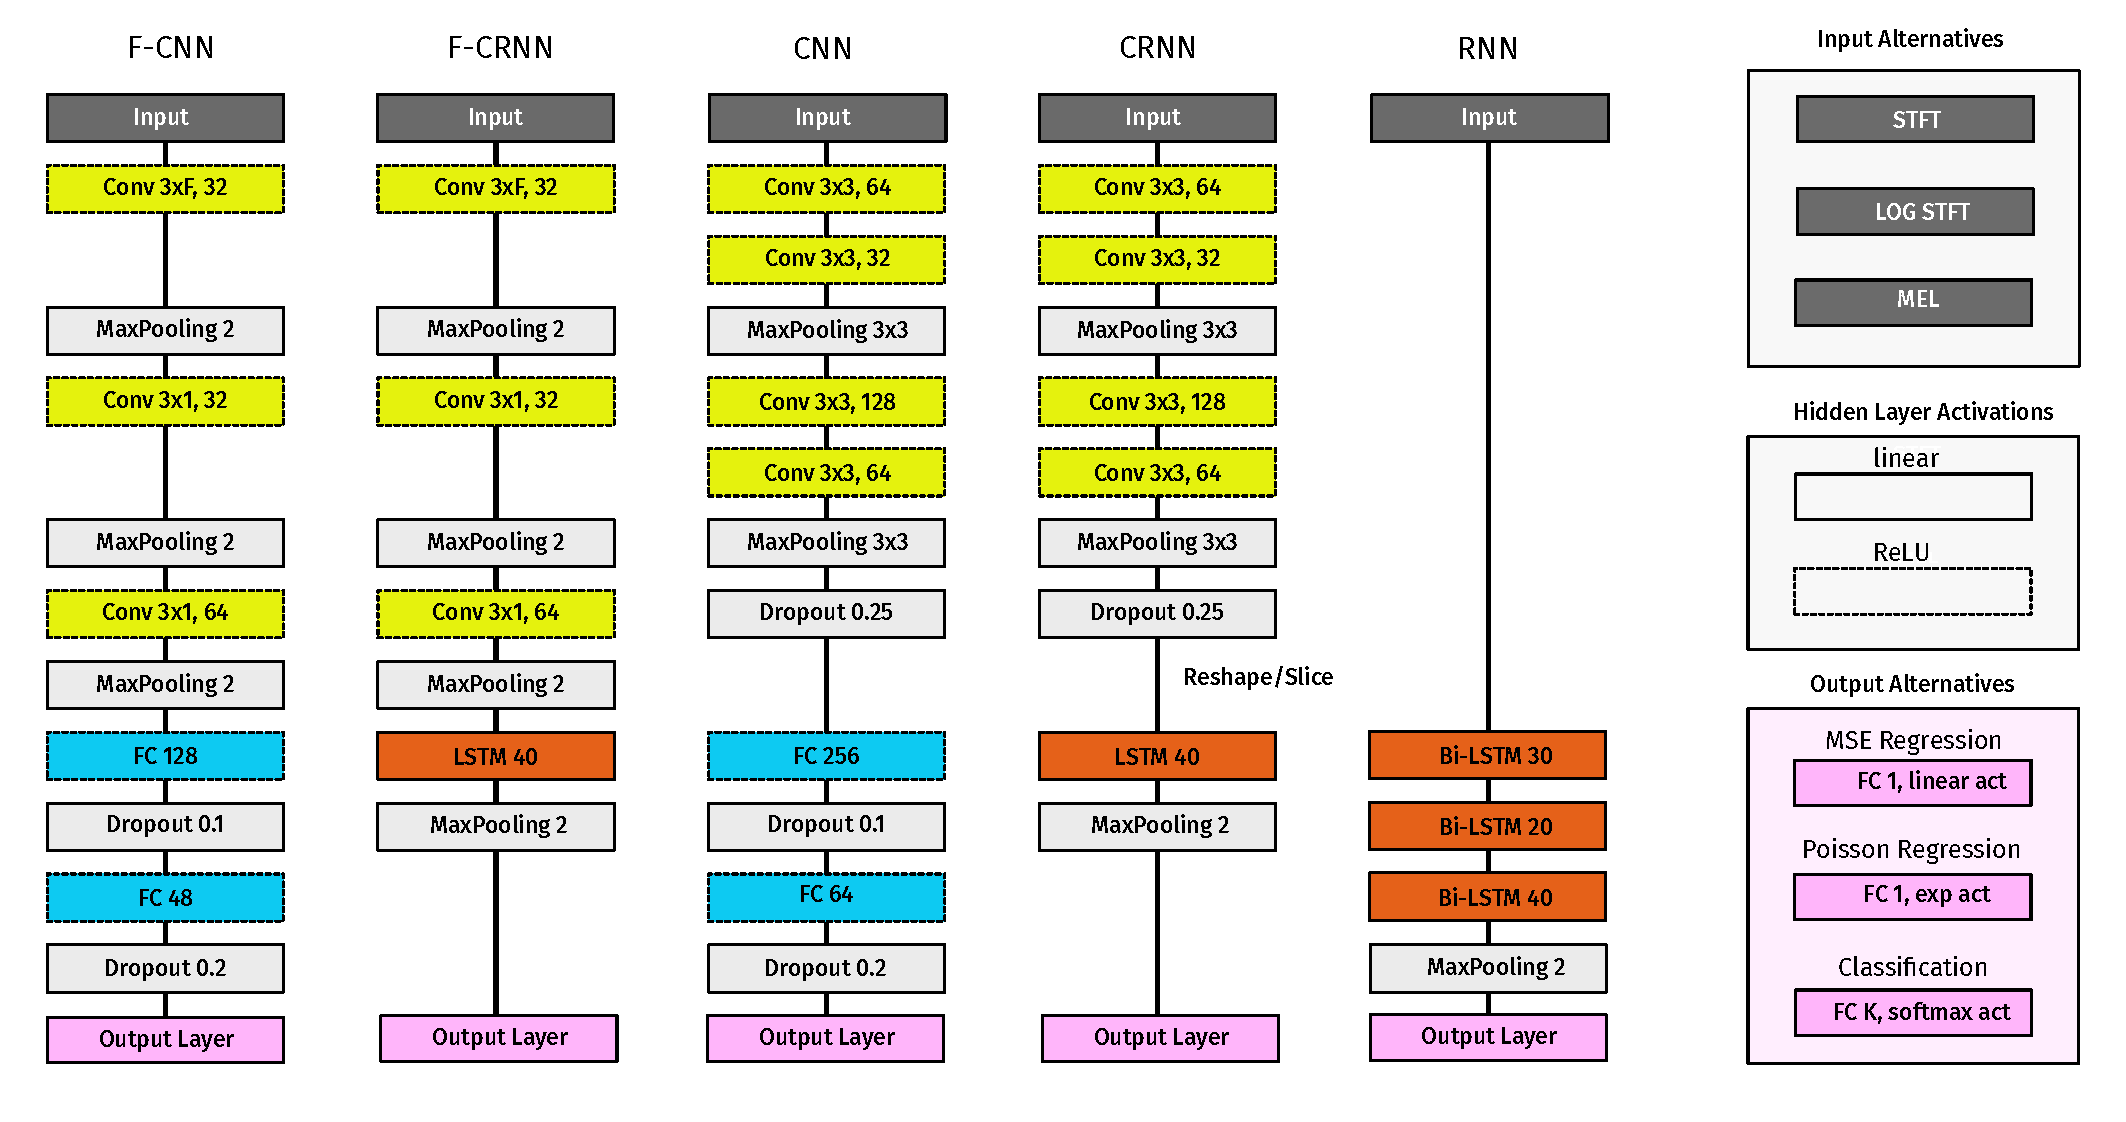
\includegraphics[width=0.9\textwidth]{Chapters/dsc/figures/networkoverview.pdf}
\caption{Overview of the proposed Architectures.}%
\label{fig:networkoverview}%
\end{figure*}

%!TEX root = ../stoeter_sourcecount.tex
\section{Training}%
\label{sec:training}

To successfully train and evaluate the proposed DNNs, due to the number of parameters, a large amount of training data is required.
In this section we introduce relevant speech corpora and describe how the training dataset was assembled.

\subsection{Speech Corpora and Annotations}%
\label{ssec:corpus}
% * Libri Speech
% * Describe the used VAD
To date many available speech datasets contain recordings where only a single speaker is active.
Datasets that include overlapped speech segments, either lack accurate annotations because the annotation of speech onsets and offsets in mixtures is cumbersome for humans as shown in Section~\ref{sec:introduction} or lack a controlled auditory environment such as in TV/broadcasting scenarios~\cite{Gravier12}.
Since a realistic dataset of fully overlapped speakers is not available, we  chose to generate synthetic mixtures.
We recognize that in a simulated ``cocktail-party'' environment, mixtures lack the conversational aspect of human communication but provide a controlled environment which helps to understand how a DNN solves the count estimation problem.
As we aim for a speaker independent solution, we selected a speech corpus with a high number of different speakers instead of large number of utterances, yielding to a larger number of unique mixtures.
For training we selected \emph{LibriSpeech clean-360}\ \cite{panayotov15} which includes 363 hours of clean speech of English utterances from 921 speakers (439 female and 482 male speakers) sampled at 16 kHz.
% Compared to \emph{LibriSpeech}, \emph{TIMIT} is of lower recording quality and \emph{THCHS} represents mandarin speech.
% \par
% As revealed in Equation~\ref{eq:definition_k}, the maximum number of concurrent speakers \(cardinality\) requires annotation of the activity of each individual speaker.
% Even though many corpora come with word and phonemes annotation, they often are not consistent across different corpora.
% We therefore generated annotations based on a voice activity detection algorithm (VAD). As we rely on a robust VAD estimate, we found the implementation from the \emph{Chromium Web Browser} as part of the WebRTC Standard~\footnote{WebRTC 1.0: Real-time Communication Between Browsers W3C Editor's Draft 05 June 2017} to yield good results.
In the further course of this work (see Section~\ref{sec:evaluation}), we also present the results from test sets of two other datasets as listed in Table~\ref{tab:corpora}.
Furthermore, we included non-speech examples from the TUT Acoustic Scenes dataset~\cite{Mesaros16} in our training data to avoid using zero input samples for \(\cardinality = 0\) to increase the robustness against noise.

% \subsection{Training Data Set}%
% \label{ssec:train}
%
% To generate a single training sample, a tuples of speech mixtures and their ground truth speaker count \(\cardinality \), we draw a unique set of \(\cardinality \) speakers from the corpus.
% For each of the speakers we then select a random utterance, resampled to 16 kHz sampling rate and apply VAD.\@
% The VAD method was configured using default parameters using a hop size of 10~ms.
% Further, the VAD estimate was used to remove silence in the beginning and the end of an utterance recording.
% In the next step, more utterances from the same speaker are drawn from the corpus until the desired duration is reached.
% Both, the audio recording and the VAD annotation of each utterance is concatenated.
% The procedure is repeated for all speaker so that \(\cardinality \) time domain signals are created.
% Signals are mixed according to Equation~\ref{eq:mixing_model} and peak normalised to avoid clipping.
% Mixtures are then transformed to a time-frequency matrix \(X \in D \times F\).
% The VAD matrix \(v_{nl}\) is upsampled in temporal direction using nearest neighbour interpolation to match \(D\).
% The ground truth output \(\cardinality \) is then computed based on Equation~\ref{eq:definition_k}.
% \par
% We follow the proposal of~\cite{wang15} and include non-speech examples in our training data to avoid using zero input samples for \(\cardinality = 0\) and also to increase the robustness against noise.
% We used the TUT Acoustic Scenes dataset~\cite{Mesaros16} to create training samples using the same procedure as described above.
% As environmental sounds could include speech, we omitted obvious subsets such as \texttt{cafe/restaurant}, \texttt{grocery store} and \texttt{metro station}.
% Additionally we used the VAD to verify if any sample contains speech.
\begin{table}
  \centering
  \caption{Overview of speech corpora used in this work.}%
\label{tab:corpora}
\begin{tabular}{llrrr}
  \toprule
  & & \multicolumn{3}{c}{Number of Speakers} \\
  \cmidrule(r){3-5}
  Name & Language &  Train & Valid. & Test\\
  \midrule
  LibriSpeech~\cite{panayotov15} & English & 921 & 40 & 40 \\
  TIMIT~\cite{TIMIT93} & English & 462 & 24 & 168 \\
  THCHS~\cite{THCHS15} & Mandarin & 30 & 10 & 10 \\
  \bottomrule
  \end{tabular}
\end{table}

\par
A single training tuple \( \left\{\mathbf{X}, k\right\} \) is generated by a synthetic speech mixture and their ground truth speaker count \(\cardinality \).
The mixtures are formed from random utterances of different speakers where silence in the beginning and end was removed.
Signals are mixed according to Equation~\ref{eq:mixing_model}, peak normalized and then transformed to a time-frequency matrix \(X \in D \times F\).
Based on a voice activity detection algorithm (VAD), we used an implementation based on the WebRTC Standard~\cite{webrtc} where we computed the ground truth output \(\cardinality \) via  Equation~\ref{eq:definition_k}.
All samples are normalized to the average Euclidean norm of \(duration\) frames to be robust against gain variations as proposed by~\cite{Uhlich15}.
Furthermore the data was scaled to zero mean and unit standard deviation across the frequency dimension \(F\) over the full training data.
Scaling parameters were saved for validation and test.

% \subsubsection{Standardization, Normalization}%
% \label{ssec:norm}
%
% As our application more closely relates to source separation we want our trained DNN system to be robust against gain variations.
% We therefore find it important that the DNN can not leverage the gain factors of the mixture.
% We found that the averaged energy of one bin across \(duration\) already is a solid indicator for the number of speakers.
% In fact, in early experiments of the methods described in~\cite{sayoud10, andrei15} we were only able to reproduce their results when no normalization was applied.
% To accommodate these findings, we normalize \(\mathbf{X}\) to the average Euclidean norm of \(duration\) frames as proposed by~\cite{Uhlich15}.
% Additionally, as common in machine learning, we scale the normalised input representation so that the feature dimension \(F\) have zero mean and unit variance/standard deviation across the whole training dataset (Standardization).

\subsection{Training Procedure}%
\label{ssec:parameters}
% * Optimizer
% other things
% To train each network we use Poisson sampling to balance the number of samples \(T_{ \cardinality}\) for each \(\cardinality \).
For all experiments we chose a medium sized training dataset of \(\cardinality \in \textrm{\{0, \ldots, 10\}}\) forming a total of \(T_{\textrm{train}} = 20.020\) mixtures  (1820 per \(k\)), each containing 10 seconds of audio, resulting in 55.55 hours of training material.
For each sample fed into the network, we select a random excerpt of duration \(D\) from each mixture.
That way, for each epoch, the network is seeing slightly different samples, reducing the number of redundant samples and thus helping to speed up the stochastic gradient based training process.
\footnote{Note that for the validation and testing, excerpts are fixed.}
A similar training procedure is detailed in~\cite{schluter16, stoeter17}.
Each architecture is trained using the ADAM optimizer~\cite{kingma14} (learning rate: \(1 \cdot 10^{-3}\), \(\beta_1=0.9\), \(\beta_2=0.999\), \(\epsilon=1 \cdot 10^{-8}\)) using mini-batches of size 32.
Our training procedure verifies that all samples within a batch are from a different set of speakers.
In addition to the training dataset, we created a fully separated validation dataset of \(T_{\textrm{valid}} = 5720\) samples using a different set of speakers from \emph{LibriSpeech dev-clean}.
Early stopping (\(patience = 10\)) is applied by monitoring the validation loss to reduce the effect of overfitting.
% As we are interested in evaluating different input durations, we need to accommodate this our training procedure where we, instead of using the full duration of one input sample, may select an excerpt of duration \(D\).
% Now instead iterating with hop size of 1 resulting in many redundant (slightly shifted) samples, we instead randomly select the offset of this excerpt for each sample.
% This procedure verifies that all samples within a batch are from different speakers.
% After every epoch the offsets are being reset so that each epoch is seeing slightly different samples (in different order) of the same training dataset.
% Note that this is not the case for the evaluation and test dataset where the offsets are fixed using an initial seed.
% We found this procedure (also used in~\cite{schluter16}) help to speed up the stochastic gradient based training process.
% Additionally it allows us to evaluate on different excerpt durations \(D\), while keeping the training dataset fixed.
Training never exceeded more than 50 epochs.
\par
We used the Keras~\cite{chollet2015keras} framework and trained on multiple instances of Nvidia GTX 1080 architecture.

%!TEX root = ../stoeter_sourcecount.tex
\section{Model Selection}%
\label{sec:hyperparameters}
% Describe popular Input representations and why MFCCs are not used in
% experiments, MEL  STFT, LOG STFT
%
% * All mixtures have the same 0dB SNR to all others
% * Trained on 20.020 Libri Speech Mixtures
% * Number Speakers [0, 1, 2, ..., 10]
% * Temporal Context (5s)
% * Different Input Representations (STFT 400, MEL40, log(STFT + 1)))
% * Different Output Objectives (classification, regression, p-regression)
%
% * --> Fix Input Representation to STFT because of little influence
% * --> Fix Output Objective to Classification for best overall performance

In this section we evaluate of three configurations of our proposed architectures, introduced in Section~\ref{sec:supervised_learning}.
Besides the architecture we investigate different input representations as well as the three proposed output distributions (see Section~\ref{sec:problem_formulation}).
The goal of this is to determine the effect of these parameters and fix them to select a final trained network (model) based on these parameters.
\par
% maybe move this down to "model comparison?"
To allow for a controlled test environment and at the same time limit the number of training iterations, we fix certain parameters:
In this experiment all speakers were mixed to 0~dB SNR.\@
Furthermore, the input duration \(D\) was fixed to five seconds.
For all experimental parameters we repeated the training three times with different random seeds for each run and report averaged results to minimize random effects caused by early stopping.
We used the \emph{LibriSpeech} dataset for both training and validation and
performed evaluation of all models on \(T_{\textrm{test}} = 5720\) unique and unseen speaker mixtures from \emph{LibriSpeech test-clean} set with \(k_{\max} = 10\).
\par
% \subsection{Input Representations}
% Up to date, most discriminative models for speech applications rely on  time-frequency (TF) magnitude representations.
% This is because, compared to raw time-domain models, TF models allow for faster training due to less data redundancy leading to generally fewer trainable parameters or shorter training duration.
Several well established input representations were evaluated in~\cite{stoeter17} such as (linear or logarithmically scaled) Short-time Fourier transform (STFT), Mel filter bank outputs (MEL), Mel Frequency Cepstral Coefficients (MFCC) representations, typically chosen for speech applications.

% \begin{table}
% \caption{Speech related Input representations}
% \label{tab:inputrep}
%   \centering
% \begin{tabular}{rll}
% \toprule
% References & Task & Representation \\
% \midrule
% \cite{geiger13, hagerer17} & Overlap Detection/VAD & MFCC \\
% \cite{Graves13, sainath15, marchi17} & ASR & MEL \\
% \cite{amodei16} & ASR & STFT \\
% \cite{schluter15, schluter16} & Singing Voice AD & \(\log(1 + \mathbf{X})\) \\
% \bottomrule
% \end{tabular}
% \end{table}

% As for the task of estimating the number of speakers, we assume that a fine frequency resolution is needed to discriminate time frequency bins with overlapped speech segments from those that only belong to a single speaker.
Even though MFCCs are used in related tasks and are included in our baseline evaluations, they are known to perform poorly when used in CNNs~\cite{Seltzer13}.
This is why we decided to not to use the MFCCs as an input for the proposed architectures.
The remaining input representations are identical to those listed in~\cite{stoeter17}:

\noindent\textbf{1) STFT}: magnitude of the Short-time Fourier transform computed using Hann-windows.
A frame length of 25~ms has been used.
The resulting input is \(X \in \mathbb{R}^{500 \times 201}\).\\
\textbf{2) LOGSTFT}: logarithmically scaled magnitudes from STFT representation using \(\log(1 + STFT)\).
The resulting input is \(X \in \mathbb{R}^{500 \times 201}\).\\
\textbf{3) MEL}: compute mapping from the STFT output directly onto Mel basis using 40 triangular filters.
The resulting input is \(X \in \mathbb{R}^{500 \times 40}\).
\par
Before feature transformation, all input files were re-sampled to 16 kHz sampling rate. All features are computed using a hop size of 10~ms.

\subsection{Metric}%
\label{ssec:metrics}

Whereas the intermediate output \(y\) is treated as either a classification or a regression problem (see Section~\ref{sec:problem_formulation}) we evaluate the final output \(\cardinality \) as a discrete regression problem.
We therefore employ the mean absolute error (MAE) being the most accessible metric, also commonly used for other count related tasks (c.f.~\cite{zhang15, Rezatofigh16}).
Since the MAE is based on the true count \(\cardinality \), we also present the individual mean absolute count error as:

\begin{equation}
  \mbox{MAE}(k) = \frac{1}{T_{\textrm{test}}} \sum_{t=1}^{T_\textrm{test}}\left| \hat{k} - k \right|.
\end{equation}

which is then averaged

\begin{equation}
  \mbox{MAE} = \frac{1}{k_{\max}} \sum_{k=0}^{k_{\max}} \mbox{MAE}(k).
\end{equation}

% * Mean Speaker Count Distance
% * Accuracy
% * Accuracy +/- 1
% * Response

\subsection{Model Comparison}%
\label{ssec:model_comparsion}

% \begin{figure*}[ht!]
%   \begin{subfigure}[b]{0.30\textwidth}
%       \centering
%       \begin{adjustbox}{width=\textwidth}
%         % This file was created by matplotlib2tikz v0.6.13.
\begin{tikzpicture}

% colors from colorbrewer Set3
\definecolor{color0}{rgb}{0.917647058823529,0.917647058823529,0.949019607843137}
\definecolor{color1}{RGB}{191,91,23}
\definecolor{color3}{RGB}{190,174,212}
\definecolor{color2}{RGB}{253,192,134}

\begin{axis}[
xlabel={k},
ylabel={MAE},
xmin=-0.5, xmax=10.5,
ymin=-0.05, ymax=0.9,
ytick={-0.1,0,0.1,0.2,0.3,0.4,0.5,0.6,0.7,0.8,0.9},
yticklabels={0.0,0.0,0.1,0.2,0.3,0.4,0.5,0.6,0.7,0.8,0.9},
xtick distance=1,
tick align=outside,
tick pos=left,
ymajorgrids,
xmajorgrids,
grid style={line width=.1pt, draw=gray!20},
major grid style={line width=.2pt,draw=gray!20},
axis line style={black},
legend style={at={(0.03,0.97)}, anchor=north west, draw=none, fill==gray!0},
legend cell align={left},
legend entries={{MEL40},{STFT},{STFTLOG}}
]
\addplot [only marks, draw=color1, fill=color1, colormap/blackwhite]
table{%
x                      y
-3.750000000000001e-02 +1.282051285115891e-03
+9.625000000000000e-01 +4.378956559182671e-02
+1.962500000000000e+00 +1.698966412812240e-01
+2.962500000000000e+00 +2.904593644946708e-01
+3.962500000000000e+00 +3.819121458168999e-01
+4.962500000000000e+00 +5.342699044052212e-01
+5.962500000000000e+00 +6.399449048893949e-01
+6.962500000000000e+00 +7.022138688498571e-01
+7.962500000000000e+00 +6.717410322614437e-01
+8.962500000000000e+00 +6.421099899821276e-01
+9.962500000000000e+00 +7.441498321916922e-01
};
\addplot [line width=2.00pt, color1, forget plot]
table {%
-0.0375 0.00128205128511589
0.9625 0.0437895655918267
1.9625 0.169896641281224
2.9625 0.290459364494671
3.9625 0.3819121458169
4.9625 0.534269904405221
5.9625 0.639944904889395
6.9625 0.702213868849857
7.9625 0.671741032261444
8.9625 0.642109989982128
9.9625 0.744149832191692
};
\addplot [line width=2.00pt, color1, forget plot]
table {%
-0.0375 0.0002991452993443
-0.0375 0.00290598291171611
};
\addplot [line width=2.00pt, color1, forget plot]
table {%
0.9625 0.0292021391029433
0.9625 0.0628356254969424
};
\addplot [line width=2.00pt, color1, forget plot]
table {%
1.9625 0.148319336806491
1.9625 0.1932881148387
};
\addplot [line width=2.00pt, color1, forget plot]
table {%
2.9625 0.260852964485001
2.9625 0.322079899352019
};
\addplot [line width=2.00pt, color1, forget plot]
table {%
3.9625 0.348403317338685
3.9625 0.418488374525981
};
\addplot [line width=2.00pt, color1, forget plot]
table {%
4.9625 0.490396980724153
4.9625 0.580383148183019
};
\addplot [line width=2.00pt, color1, forget plot]
table {%
5.9625 0.59489899164649
5.9625 0.690870064470585
};
\addplot [line width=2.00pt, color1, forget plot]
table {%
6.9625 0.654216791062228
6.9625 0.75059524217121
};
\addplot [line width=2.00pt, color1, forget plot]
table {%
7.9625 0.629482719495514
7.9625 0.712939632123146
};
\addplot [line width=2.00pt, color1, forget plot]
table {%
8.9625 0.5712637464472
8.9625 0.720740745223197
};
\addplot [line width=2.00pt, color1, forget plot]
table {%
9.9625 0.603217593893058
9.9625 0.889956860029537
};
\addplot [only marks, draw=color2, fill=color2, colormap/blackwhite]
table{%
x                      y
+0.000000000000000e+00 +4.017094149429383e-03
+1.000000000000000e+00 +2.165466058294658e-02
+2.000000000000000e+00 +1.097760553809459e-01
+3.000000000000000e+00 +2.075775420503098e-01
+4.000000000000000e+00 +3.075366057808496e-01
+5.000000000000000e+00 +4.309067676908769e-01
+6.000000000000000e+00 +5.230027550672368e-01
+7.000000000000000e+00 +6.100250622981175e-01
+8.000000000000000e+00 +5.915135611073551e-01
+9.000000000000000e+00 +5.562738505022561e-01
+1.000000000000000e+01 +6.068181814770105e-01
};
\addplot [line width=2.00pt, color2, forget plot]
table {%
0 0.00401709414942938
1 0.0216546605829466
2 0.109776055380946
3 0.20757754205031
4 0.30753660578085
5 0.430906767690877
6 0.523002755067237
7 0.610025062298117
8 0.591513561107355
9 0.556273850502256
10 0.60681818147701
};
\addplot [line width=2.00pt, color2, forget plot]
table {%
0 0.00141025642932265
0 0.00777884649395501
};
\addplot [line width=2.00pt, color2, forget plot]
table {%
1 0.015104780559566
1 0.0292981881977767
};
\addplot [line width=2.00pt, color2, forget plot]
table {%
2 0.0935389754212398
2 0.126616063651554
};
\addplot [line width=2.00pt, color2, forget plot]
table {%
3 0.184214762288727
3 0.232517668003831
};
\addplot [line width=2.00pt, color2, forget plot]
table {%
4 0.283712317184782
4 0.329804048656288
};
\addplot [line width=2.00pt, color2, forget plot]
table {%
5 0.401557044723647
5 0.465348019600485
};
\addplot [line width=2.00pt, color2, forget plot]
table {%
6 0.490907942142724
6 0.554963269541031
};
\addplot [line width=2.00pt, color2, forget plot]
table {%
7 0.571706349037544
7 0.650759191716972
};
\addplot [line width=2.00pt, color2, forget plot]
table {%
8 0.557388451102525
8 0.628085083916509
};
\addplot [line width=2.00pt, color2, forget plot]
table {%
9 0.510563413293006
9 0.60849158311509
};
\addplot [line width=2.00pt, color2, forget plot]
table {%
10 0.507567340790322
10 0.711869740708408
};
\path [draw=white, fill opacity=0] (axis cs:0,-0.0552693502854651)
--(axis cs:0,0.934967631949299);

\path [draw=white, fill opacity=0] (axis cs:1,-0.0552693502854651)
--(axis cs:1,0.934967631949299);

\path [draw=white, fill opacity=0] (axis cs:-0.5,0)
--(axis cs:10.5,0);

\path [draw=white, fill opacity=0] (axis cs:-0.5,1)
--(axis cs:10.5,1);

\addplot [only marks, draw=color3, fill=color3, colormap/blackwhite]
table{%
x                      y
+3.750000000000001e-02 +4.491453003381084e-02
+1.037500000000000e+00 +4.894127914890618e-02
+2.037500000000000e+00 +1.479328153983824e-01
+3.037500000000000e+00 +2.669022376087070e-01
+4.037500000000000e+00 +3.958656320969263e-01
+5.037500000000000e+00 +5.179225227638933e-01
+6.037500000000000e+00 +6.520202012977215e-01
+7.037500000000000e+00 +7.256892264536648e-01
+8.037500000000000e+00 +6.448818897898534e-01
+9.037500000000000e+00 +5.645342315434071e-01
+1.003750000000000e+01 +5.662037049329240e-01
};
\addplot [line width=2.00pt, color3, forget plot]
table {%
0.0375 0.0449145300338108
1.0375 0.0489412791489062
2.0375 0.147932815398382
3.0375 0.266902237608707
4.0375 0.395865632096926
5.0375 0.517922522763893
6.0375 0.652020201297722
7.0375 0.725689226453665
8.0375 0.644881889789853
9.0375 0.564534231543407
10.0375 0.566203704932924
};
\addplot [line width=2.00pt, color3, forget plot]
table {%
0.0375 0.00563675216719425
0.0375 0.0978333334729233
};
\addplot [line width=2.00pt, color3, forget plot]
table {%
1.0375 0.0240973587901605
1.0375 0.083095393889988
};
\addplot [line width=2.00pt, color3, forget plot]
table {%
2.0375 0.119852497411666
2.0375 0.180880703087784
};
\addplot [line width=2.00pt, color3, forget plot]
table {%
3.0375 0.236119944983176
3.0375 0.298233213870577
};
\addplot [line width=2.00pt, color3, forget plot]
table {%
4.0375 0.354053618227044
4.0375 0.434679154426463
};
\addplot [line width=2.00pt, color3, forget plot]
table {%
5.0375 0.46628033370452
5.0375 0.5704150723004
};
\addplot [line width=2.00pt, color3, forget plot]
table {%
6.0375 0.599070247832217
6.0375 0.705386820743399
};
\addplot [line width=2.00pt, color3, forget plot]
table {%
7.0375 0.663815792690194
7.0375 0.786649962138935
};
\addplot [line width=2.00pt, color3, forget plot]
table {%
8.0375 0.588227250151147
8.0375 0.700395887889496
};
\addplot [line width=2.00pt, color3, forget plot]
table {%
9.0375 0.508768798929406
9.0375 0.623634119981668
};
\addplot [line width=2.00pt, color3, forget plot]
table {%
10.0375 0.464126683435331
10.0375 0.659747474216276
};
\end{axis}

\end{tikzpicture}

%       \end{adjustbox}
%       \caption{by feature representations.}%
%       \label{fig:ssec:exp_fixed_gains/A}
%   \end{subfigure}\hfill%
%   \begin{subfigure}[b]{0.30\textwidth}
%       \centering
%       \begin{adjustbox}{width=\textwidth}
%         % This file was created by matplotlib2tikz v0.6.13.
\begin{tikzpicture}

\definecolor{color0}{rgb}{0.917647058823529,0.917647058823529,0.949019607843137}
\definecolor{color1}{RGB}{102,194,165}
\definecolor{color3}{RGB}{252,141,98}
\definecolor{color2}{RGB}{141,160,203}

\begin{axis}[
xlabel={k},
ylabel={MAE},
xmin=-0.5, xmax=10.5,
ymin=-0.05, ymax=0.9,
ytick={-0.1,0,0.1,0.2,0.3,0.4,0.5,0.6,0.7,0.8,0.9},
yticklabels={0.0,0.0,0.1,0.2,0.3,0.4,0.5,0.6,0.7,0.8,0.9},
xtick distance=1,
tick align=outside,
tick pos=left,
ymajorgrids,
xmajorgrids,
axis line style={black},
grid style={line width=.1pt, draw=gray!20},
major grid style={line width=.2pt,draw=gray!20},
legend style={at={(0.03,0.97)}, anchor=north west, draw=none, fill==gray!0},
legend entries={{Classification},{Gaussian Regr.},{Poisson Regr.}},
legend cell align={left}
]
\addplot [only marks, draw=color1, fill=color1, colormap/blackwhite]
table{%
x                      y
-3.750000000000001e-02 +3.735042735042735e-02
+9.625000000000000e-01 +2.086880593756822e-02
+1.962500000000000e+00 +9.780361757105942e-02
+2.962500000000000e+00 +2.061248527679623e-01
+3.962500000000000e+00 +3.319121447028424e-01
+4.962500000000000e+00 +4.427415921668795e-01
+5.962500000000000e+00 +5.417355371900826e-01
+6.962500000000000e+00 +6.838345864661655e-01
+7.962500000000000e+00 +7.204724409448819e-01
+8.962500000000000e+00 +7.120987654320987e-01
+9.962500000000000e+00 +3.478956228956228e-01
};
\addplot [line width=2.00pt, color1, forget plot]
table {%
-0.0375 0.0373504273504274
0.9625 0.0208688059375682
1.9625 0.0978036175710594
2.9625 0.206124852767962
3.9625 0.331912144702842
4.9625 0.44274159216688
5.9625 0.541735537190083
6.9625 0.683834586466165
7.9625 0.720472440944882
8.9625 0.712098765432099
9.9625 0.347895622895623
};
\addplot [line width=2.00pt, color1, forget plot]
table {%
-0.0375 0.00153739316239316
-0.0375 0.0895363247863248
};
\addplot [line width=2.00pt, color1, forget plot]
table {%
0.9625 0.0127919668194717
0.9625 0.0316961362148003
};
\addplot [line width=2.00pt, color1, forget plot]
table {%
1.9625 0.0817797157622739
1.9625 0.114736218776916
};
\addplot [line width=2.00pt, color1, forget plot]
table {%
2.9625 0.182602080879466
2.9625 0.231887514723204
};
\addplot [line width=2.00pt, color1, forget plot]
table {%
3.9625 0.29969315245478
3.9625 0.365779500430663
};
\addplot [line width=2.00pt, color1, forget plot]
table {%
4.9625 0.399341209025117
4.9625 0.485740740740741
};
\addplot [line width=2.00pt, color1, forget plot]
table {%
5.9625 0.502793847566575
5.9625 0.579757805325987
};
\addplot [line width=2.00pt, color1, forget plot]
table {%
6.9625 0.631313700918964
6.9625 0.745908521303258
};
\addplot [line width=2.00pt, color1, forget plot]
table {%
7.9625 0.66682195975503
7.9625 0.773801399825022
};
\addplot [line width=2.00pt, color1, forget plot]
table {%
8.9625 0.663826038159372
8.9625 0.758792368125701
};
\addplot [line width=2.00pt, color1, forget plot]
table {%
9.9625 0.283256523569024
9.9625 0.418800505050505
};
\addplot [only marks, draw=color2, fill=color2, colormap/blackwhite]
table{%
x                      y
+0.000000000000000e+00 +1.235042760510825e-02
+1.000000000000000e+00 +7.290984498750833e-02
+2.000000000000000e+00 +1.817398789856169e-01
+3.000000000000000e+00 +2.903023165133264e-01
+4.000000000000000e+00 +3.893195516533322e-01
+5.000000000000000e+00 +5.250319321950276e-01
+6.000000000000000e+00 +6.450872368282742e-01
+7.000000000000000e+00 +6.927318334579468e-01
+8.000000000000000e+00 +6.023184604114956e-01
+9.000000000000000e+00 +5.145679036776225e-01
+1.000000000000000e+01 +7.327020216319297e-01
};
\addplot [line width=2.00pt, color2, forget plot]
table {%
0 0.0123504276051083
1 0.0729098449875083
2 0.181739878985617
3 0.290302316513326
4 0.389319551653332
5 0.525031932195028
6 0.645087236828274
7 0.692731833457947
8 0.602318460411496
9 0.514567903677623
10 0.73270202163193
};
\addplot [line width=2.00pt, color2, forget plot]
table {%
0 0.00534081213764795
0 0.0241025645566535
};
\addplot [line width=2.00pt, color2, forget plot]
table {%
1 0.0466262830175563
1 0.110413665477342
};
\addplot [line width=2.00pt, color2, forget plot]
table {%
2 0.155333763578286
2 0.211202626282142
};
\addplot [line width=2.00pt, color2, forget plot]
table {%
3 0.257034745460583
3 0.324860619132717
};
\addplot [line width=2.00pt, color2, forget plot]
table {%
4 0.34692829568353
4 0.432953272768193
};
\addplot [line width=2.00pt, color2, forget plot]
table {%
5 0.478991059346331
5 0.574425296684106
};
\addplot [line width=2.00pt, color2, forget plot]
table {%
6 0.590747243298425
6 0.699374426702658
};
\addplot [line width=2.00pt, color2, forget plot]
table {%
7 0.634959278139803
7 0.754830837696791
};
\addplot [line width=2.00pt, color2, forget plot]
table {%
8 0.562505469305648
8 0.6433584856987
};
\addplot [line width=2.00pt, color2, forget plot]
table {%
9 0.468725030223529
9 0.570103260063463
};
\addplot [line width=2.00pt, color2, forget plot]
table {%
10 0.624493893070353
10 0.840917507157558
};
% \path [draw=white, fill opacity=0] (axis cs:0,-0.0600185928210457)
% --(axis cs:0,1.00006922752411);
%
% \path [draw=white, fill opacity=0] (axis cs:1,-0.0600185928210457)
% --(axis cs:1,1.00006922752411);
%
% \path [draw=white, fill opacity=0] (axis cs:-0.5,0)
% --(axis cs:10.5,0);
%
% \path [draw=white, fill opacity=0] (axis cs:-0.5,1)
% --(axis cs:10.5,1);

\addplot [only marks, draw=color3, fill=color3, colormap/blackwhite]
table{%
x                      y
+3.750000000000001e-02 +5.128205128205128e-04
+1.037500000000000e+00 +2.060685439860293e-02
+2.037500000000000e+00 +1.480620155038760e-01
+3.037500000000000e+00 +2.685119748723989e-01
+4.037500000000000e+00 +3.640826873385014e-01
+5.037500000000000e+00 +5.153256704980842e-01
+6.037500000000000e+00 +6.281450872359963e-01
+7.037500000000000e+00 +6.613617376775270e-01
+8.037500000000000e+00 +5.853455818022747e-01
+9.037500000000000e+00 +5.362514029180696e-01
+1.003750000000000e+01 +8.365740740740741e-01
};
\addplot [line width=2.00pt, color3, forget plot]
table {%
0.0375 0.000512820512820513
1.0375 0.0206068543986029
2.0375 0.148062015503876
3.0375 0.268511974872399
4.0375 0.364082687338501
5.0375 0.515325670498084
6.0375 0.628145087235996
7.0375 0.661361737677527
8.0375 0.585345581802275
9.0375 0.53625140291807
10.0375 0.836574074074074
};
\addplot [line width=2.00pt, color3, forget plot]
table {%
0.0375 0.000170940170940171
0.0375 0.000982905982905983
};
\addplot [line width=2.00pt, color3, forget plot]
table {%
1.0375 0.0122647893473041
1.0375 0.0345797860729098
};
\addplot [line width=2.00pt, color3, forget plot]
table {%
2.0375 0.12656976744186
2.0375 0.169559646856158
};
\addplot [line width=2.00pt, color3, forget plot]
table {%
3.0375 0.240591872791519
3.0375 0.298862387122104
};
\addplot [line width=2.00pt, color3, forget plot]
table {%
4.0375 0.332558139534884
4.0375 0.39405684754522
};
\addplot [line width=2.00pt, color3, forget plot]
table {%
5.0375 0.476749680715198
5.0375 0.554259259259259
};
\addplot [line width=2.00pt, color3, forget plot]
table {%
6.0375 0.587143021120294
6.0375 0.676090449954086
};
\addplot [line width=2.00pt, color3, forget plot]
table {%
7.0375 0.614816207184628
7.0375 0.704314954051796
};
\addplot [line width=2.00pt, color3, forget plot]
table {%
8.0375 0.549119641294838
8.0375 0.623103674540682
};
\addplot [line width=2.00pt, color3, forget plot]
table {%
9.0375 0.475597081930415
9.0375 0.597627384960718
};
\addplot [line width=2.00pt, color3, forget plot]
table {%
10.0375 0.727001262626263
10.0375 0.951883417508417
};
\end{axis}

\end{tikzpicture}

%       \end{adjustbox}
%       \caption{by output distribution.}%
%       \label{fig:ssec:exp_fixed_gains/B}
%   \end{subfigure}\hfill%
%   \begin{subfigure}[b]{0.30\textwidth}
%       \centering
%       \begin{adjustbox}{width=\textwidth}
%         % This file was created by matplotlib2tikz v0.6.13.
\begin{tikzpicture}

\definecolor{color0}{rgb}{0.917647058823529,0.917647058823529,0.949019607843137}

\begin{axis}[
xlabel={k},
ylabel={MAE},
xmin=-0.5, xmax=10.5,
ymin=-0.05, ymax=0.9,
ytick={-0.1,0,0.1,0.2,0.3,0.4,0.5,0.6,0.7,0.8,0.9},
yticklabels={0.0,0.0,0.1,0.2,0.3,0.4,0.5,0.6,0.7,0.8,0.9},
xtick distance=1,
tick align=outside,
tick pos=left,
ymajorgrids,
xmajorgrids,
axis line style={black},
grid style={line width=.1pt, draw=gray!20},
major grid style={line width=.2pt,draw=gray!20},
legend entries={{F-CNN},{CNN},{F-CRNN},{CRNN},{RNN~\cite{stoeter17}}},
legend style={at={(0.03,0.97)}, anchor=north west, draw=none, fill=gray!0},
legend cell align={left}
]
\addplot [only marks, draw=FCNN, fill=FCNN, colormap/blackwhite]
table{%
x                      y
-6.250000000000000e-02 +1.609686645533242e-02
+9.375000000000000e-01 +6.810740004287860e-02
+1.937500000000000e+00 +1.871231682694852e-01
+2.937500000000000e+00 +2.900143965558066e-01
+3.937500000000000e+00 +4.082687340469289e-01
+4.937500000000000e+00 +5.654179110829165e-01
+5.937500000000000e+00 +6.553412880013030e-01
+6.937500000000000e+00 +7.385129500517637e-01
+7.937500000000000e+00 +6.676144655364774e-01
+8.937500000000000e+00 +6.725028088197162e-01
+9.937500000000000e+00 +8.343855208151804e-01
};
\addplot [line width=2.00pt, FCNN, forget plot]
table {%
-0.0625 0.0160968664553324
0.9375 0.0681074000428786
1.9375 0.187123168269485
2.9375 0.290014396555807
3.9375 0.408268734046929
4.9375 0.565417911082917
5.9375 0.655341288001303
6.9375 0.738512950051764
7.9375 0.667614465536477
8.9375 0.672502808819716
9.9375 0.83438552081518
};
\addplot [line width=2.00pt, FCNN, forget plot]
table {%
-0.0625 0.00427350433559245
-0.0625 0.032419872278337
};
\addplot [line width=2.00pt, FCNN, forget plot]
table {%
0.9375 0.0406734335280436
0.9375 0.10157898504591
};
\addplot [line width=2.00pt, FCNN, forget plot]
table {%
1.9375 0.149366565919747
1.9375 0.233137736180939
};
\addplot [line width=2.00pt, FCNN, forget plot]
table {%
2.9375 0.254217380758762
2.9375 0.327314815066483
};
\addplot [line width=2.00pt, FCNN, forget plot]
table {%
3.9375 0.374671620453119
3.9375 0.445592879322353
};
\addplot [line width=2.00pt, FCNN, forget plot]
table {%
4.9375 0.520718039641279
4.9375 0.61367780890385
};
\addplot [line width=2.00pt, FCNN, forget plot]
table {%
5.9375 0.600531829466213
5.9375 0.715734995382986
};
\addplot [line width=2.00pt, FCNN, forget plot]
table {%
6.9375 0.673544972183909
6.9375 0.808347258480503
};
\addplot [line width=2.00pt, FCNN, forget plot]
table {%
7.9375 0.600100245278955
7.9375 0.744099954962643
};
\addplot [line width=2.00pt, FCNN, forget plot]
table {%
8.9375 0.585170224673887
8.9375 0.760961468631839
};
\addplot [line width=2.00pt, FCNN, forget plot]
table {%
9.9375 0.656660354222713
9.9375 1.02770763036244
};
\addplot [only marks, draw=CNN, fill=CNN, colormap/blackwhite]
table{%
x                      y
-3.125000000000000e-02 +1.495726509789201e-03
+9.687500000000000e-01 +1.760896459410368e-02
+1.968750000000000e+00 +1.216623599392619e-01
+2.968750000000000e+00 +2.069100901482539e-01
+3.968750000000000e+00 +2.922049940205702e-01
+4.968750000000000e+00 +4.167730962238836e-01
+5.968750000000000e+00 +5.557086000319903e-01
+6.968750000000000e+00 +5.869534927485414e-01
+7.968750000000000e+00 +5.456401261879356e-01
+8.968750000000000e+00 +5.296670419778263e-01
+9.968750000000000e+00 +6.469556705317513e-01
};
\addplot [line width=2.00pt, CNN, forget plot]
table {%
-0.03125 0.0014957265097892
0.96875 0.0176089645941037
1.96875 0.121662359939262
2.96875 0.206910090148254
3.96875 0.29220499402057
4.96875 0.416773096223884
5.96875 0.55570860003199
6.96875 0.586953492748541
7.96875 0.545640126187936
8.96875 0.529667041977826
9.96875 0.646955670531751
};
\addplot [line width=2.00pt, CNN, forget plot]
table {%
-0.03125 0.000569800578609661
-0.03125 0.00242343307596477
};
\addplot [line width=2.00pt, CNN, forget plot]
table {%
0.96875 0.0108382449495332
0.96875 0.0252510370163853
};
\addplot [line width=2.00pt, CNN, forget plot]
table {%
1.96875 0.0968938411976859
1.96875 0.149162000738605
};
\addplot [line width=2.00pt, CNN, forget plot]
table {%
2.96875 0.172551041119997
2.96875 0.243168432323684
};
\addplot [line width=2.00pt, CNN, forget plot]
table {%
3.96875 0.253718057931103
3.96875 0.335432813824626
};
\addplot [line width=2.00pt, CNN, forget plot]
table {%
4.96875 0.357010075388622
4.96875 0.480567972900403
};
\addplot [line width=2.00pt, CNN, forget plot]
table {%
5.96875 0.49686065282448
5.96875 0.629650670435721
};
\addplot [line width=2.00pt, CNN, forget plot]
table {%
6.96875 0.520739347236638
6.96875 0.652126840199934
};
\addplot [line width=2.00pt, CNN, forget plot]
table {%
7.96875 0.500136699940119
7.96875 0.588074144240187
};
\addplot [line width=2.00pt, CNN, forget plot]
table {%
8.96875 0.475188928860774
8.96875 0.57882903330265
};
\addplot [line width=2.00pt, CNN, forget plot]
table {%
9.96875 0.499768520983649
9.96875 0.791559695281866
};
\path [draw=white, fill opacity=0] (axis cs:0,-0.0642762651515782)
--(axis cs:0,1.07970686348216);

\path [draw=white, fill opacity=0] (axis cs:1,-0.0642762651515782)
--(axis cs:1,1.07970686348216);

\path [draw=white, fill opacity=0] (axis cs:-0.5,0)
--(axis cs:10.5,0);

\path [draw=white, fill opacity=0] (axis cs:-0.5,1)
--(axis cs:10.5,1);

\addplot [only marks, draw=FCRNN, fill=FCRNN, colormap/blackwhite]
table{%
x                      y
+0.000000000000000e+00 +6.346153848163752e-02
+1.000000000000000e+00 +7.218220163694986e-02
+2.000000000000000e+00 +1.653028996578414e-01
+3.000000000000000e+00 +2.925664174269669e-01
+4.000000000000000e+00 +4.153029006632313e-01
+5.000000000000000e+00 +5.485312881513033e-01
+6.000000000000000e+00 +6.603152773086178e-01
+7.000000000000000e+00 +7.562656681606015e-01
+8.000000000000000e+00 +6.770195411537229e-01
+9.000000000000000e+00 +5.510662176793674e-01
+1.000000000000000e+01 +6.087962971993969e-01
};
\addplot [line width=2.00pt, FCRNN, forget plot]
table {%
0 0.0634615384816375
1 0.0721822016369499
2 0.165302899657841
3 0.292566417426967
4 0.415302900663231
5 0.548531288151303
6 0.660315277308618
7 0.756265668160601
8 0.677019541153723
9 0.551066217679367
10 0.608796297199397
};
\addplot [line width=2.00pt, FCRNN, forget plot]
table {%
0 0.00327457266575969
0 0.152783119675935
};
\addplot [line width=2.00pt, FCRNN, forget plot]
table {%
1 0.0379811538036914
1 0.117306993108207
};
\addplot [line width=2.00pt, FCRNN, forget plot]
table {%
2 0.142825868812946
2 0.189570772423677
};
\addplot [line width=2.00pt, FCRNN, forget plot]
table {%
3 0.26108166456477
3 0.321173601928928
};
\addplot [line width=2.00pt, FCRNN, forget plot]
table {%
4 0.379186404986292
4 0.450771608875335
};
\addplot [line width=2.00pt, FCRNN, forget plot]
table {%
5 0.503400382091471
5 0.592736270459379
};
\addplot [line width=2.00pt, FCRNN, forget plot]
table {%
6 0.610785893782549
6 0.711432509583583
};
\addplot [line width=2.00pt, FCRNN, forget plot]
table {%
7 0.707322127606271
7 0.805423287159302
};
\addplot [line width=2.00pt, FCRNN, forget plot]
table {%
8 0.627726745471189
8 0.733316930837779
};
\addplot [line width=2.00pt, FCRNN, forget plot]
table {%
9 0.488881408392023
9 0.614322857952468
};
\addplot [line width=2.00pt, FCRNN, forget plot]
table {%
10 0.498625141462493
10 0.723000841983307
};
\addplot [only marks, draw=CRNN, fill=CRNN, colormap/blackwhite]
table{%
x                      y
+3.125000000000000e-02 +1.424501451631833e-03
+1.031250000000000e+00 +7.567488835640818e-03
+2.031250000000000e+00 +7.493540085798669e-02
+3.031250000000000e+00 +1.739301140378820e-01
+4.031250000000000e+00 +2.658627627782701e-01
+5.031250000000000e+00 +3.860508020218169e-01
+6.031250000000000e+00 +5.054331182119932e-01
+7.031250000000000e+00 +5.913394604825403e-01
+8.031250000000000e+00 +5.926655008150419e-01
+9.031250000000000e+00 +4.832023948219176e-01
+1.003125000000000e+01 +3.981481475209950e-01
};
\addplot [line width=2.00pt, CRNN, forget plot]
table {%
0.03125 0.00142450145163183
1.03125 0.00756748883564082
2.03125 0.0749354008579867
3.03125 0.173930114037882
4.03125 0.26586276277827
5.03125 0.386050802021817
6.03125 0.505433118211993
7.03125 0.59133946048254
8.03125 0.592665500815042
9.03125 0.483202394821918
10.03125 0.398148147520995
};
\addplot [line width=2.00pt, CRNN, forget plot]
table {%
0.03125 0.0004985754989735
0.03125 0.00270655276526948
};
\addplot [line width=2.00pt, CRNN, forget plot]
table {%
1.03125 0.00203558178730112
1.03125 0.0145546822128031
};
\addplot [line width=2.00pt, CRNN, forget plot]
table {%
2.03125 0.0569157335567367
2.03125 0.0955408415482242
};
\addplot [line width=2.00pt, CRNN, forget plot]
table {%
3.03125 0.146104894003063
3.03125 0.204166667151622
};
\addplot [line width=2.00pt, CRNN, forget plot]
table {%
4.03125 0.23291343713199
4.03125 0.2977354312345
};
\addplot [line width=2.00pt, CRNN, forget plot]
table {%
5.03125 0.348859443451997
5.03125 0.421471903264116
};
\addplot [line width=2.00pt, CRNN, forget plot]
table {%
6.03125 0.457526017299231
6.03125 0.55380509473705
};
\addplot [line width=2.00pt, CRNN, forget plot]
table {%
7.03125 0.533848510757068
7.03125 0.653164161347108
};
\addplot [line width=2.00pt, CRNN, forget plot]
table {%
8.03125 0.543070136671617
8.03125 0.643294327571819
};
\addplot [line width=2.00pt, CRNN, forget plot]
table {%
9.03125 0.423866442182048
9.03125 0.545838009867325
};
\addplot [line width=2.00pt, CRNN, forget plot]
table {%
10.03125 0.310530652987377
10.03125 0.493304572760114
};
\addplot [only marks, draw=RNN, fill=RNN, colormap/blackwhite]
table{%
x                      y
+6.250000000000000e-02 +1.210826215535890e-03
+1.062500000000000e+00 +2.517645376322615e-02
+2.062500000000000e+00 +1.636520247096787e-01
+3.062500000000000e+00 +3.114775554205700e-01
+4.062500000000000e+00 +4.272179146487926e-01
+5.062500000000000e+00 +5.550588939533989e-01
+6.062500000000000e+00 +6.481481518700176e-01
+7.062500000000000e+00 +7.234753578926187e-01
+8.062500000000000e+00 +6.972878382379093e-01
+9.062500000000000e+00 +7.017583234141570e-01
+1.006250000000000e+01 +7.070005616020540e-01
};
\addplot [line width=2.00pt, RNN, forget plot]
table {%
0.0625 0.00121082621553589
1.0625 0.0251764537632262
2.0625 0.163652024709679
3.0625 0.31147755542057
4.0625 0.427217914648793
5.0625 0.555058893953399
6.0625 0.648148151870018
7.0625 0.723475357892619
8.0625 0.697287838237909
9.0625 0.701758323414157
10.0625 0.707000561602054
};
\addplot [line width=2.00pt, RNN, forget plot]
table {%
0.0625 0.000498575503043061
0.0625 0.00206552708364109
};
\addplot [line width=2.00pt, RNN, forget plot]
table {%
1.0625 0.0152059230939088
1.0625 0.0382776697341815
};
\addplot [line width=2.00pt, RNN, forget plot]
table {%
2.0625 0.137376184544189
2.0625 0.190929156405883
};
\addplot [line width=2.00pt, RNN, forget plot]
table {%
3.0625 0.277707434068703
3.0625 0.350161955888962
};
\addplot [line width=2.00pt, RNN, forget plot]
table {%
4.0625 0.388874532062664
4.0625 0.477535531107479
};
\addplot [line width=2.00pt, RNN, forget plot]
table {%
5.0625 0.501489998066643
5.0625 0.623877187503222
};
\addplot [line width=2.00pt, RNN, forget plot]
table {%
6.0625 0.591823541416117
6.0625 0.716944064002884
};
\addplot [line width=2.00pt, RNN, forget plot]
table {%
7.0625 0.666513509922657
7.0625 0.78691347012718
};
\addplot [line width=2.00pt, RNN, forget plot]
table {%
8.0625 0.642745697520484
8.0625 0.764656240344221
};
\addplot [line width=2.00pt, RNN, forget plot]
table {%
9.0625 0.624979422747464
9.0625 0.786464645104532
};
\addplot [line width=2.00pt, RNN, forget plot]
table {%
10.0625 0.566563200983234
10.0625 0.853794893655846
};
\end{axis}

\end{tikzpicture}

%       \end{adjustbox}
%       \caption{by proposed DNN architecture.}%
%       \label{fig:ssec:exp_fixed_gains/C}
%   \end{subfigure}
%   \caption{Figure shows results of average Mean Absolute Error (MAE) on 0~\mbox{dB} SNR mixtures as described in \textsc{Experiment~\ref{ssec:model_comparsion}} per ground truth count \(k=[0\ldots10]\). Error bars show the 95\% confidence intervals. Results in (a) are averaged over factors shown in (b) and (c) and similarly for (b) and (c).}%
%   \label{fig:fixed-gain-results}
%  \end{figure*}

To find the best parameters we performed training and evaluation for different input representations and output distributions (c.f. \cite{stoeter17}) as well as all proposed architectures resulting in 135 models.
On average each model was trained 25 epochs before early stopping was engaged.
We present the results filtered by the three factors (Architecture, Input and Output) in Figure~\ref{fig:fixed-gain-results}.
One can see that the overall trend of the count error in MAE is similar regardless of the parametrization: all models are able to reliably distinguish between \(k=0\) and \(k=1\), followed by a nearly linear increase in MAE between \(k=\{1, 2\dots7\}\).
For \(k > 7\) it can be seen that the classification type models have learned the maximum of \(k\) across the dataset, hence the prediction error decreases when \(k\) reaches its maximum.
This is because classification based models intrinsically have access to the maximum number of sources determined by the output vector dimensionality.
Furthermore, one can see that all three factors have only little effect on the overall performance of the model, which is especially the case for small \(k\).
As indicated by Figure~\ref{fig:ssec:exp_fixed_gains/A}, choosing linear STFT as input representation generally results in a better performance compared to \emph{MEL40} and even \emph{LOGSTFT}.
Concerning the output distribution, a similar observation can be made about classification which outperforms Poisson regression and Gaussian regression, as indicated by Figure~\ref{fig:ssec:exp_fixed_gains/B}.
In Figure~\ref{fig:ssec:exp_fixed_gains/C} the performance of our proposed architectures are compared:
while CNN and CRNN are close, both of them perform better than full frequency band F-CNN and F-CRNN models as well as the recurrent based architecture, proposed in~\cite{stoeter17}.
However it is interesting that, despite its simplicity, the F-CNN and F-CRNN, perform similar to the Bi-LSTM architecture.
\par
The results are supported by a statistical evaluation based on mixed effect linear model (see Table~\ref{tab:mixedmodel1}) where \(k\) is modeled as a random effect (for further details we refer to~\cite{Mcculloch06}).
For a fair comparison (i.e. reducing the bias towards classification type network) of all models we only consider results for \(k = \{1, 2\dots7\}\).
These results indicate that CRNN performs statistically significantly better than the CNN.\@
Concerning the input representation we can report that using \emph{STFT} representation outperforms the log-scaled STFT as well as the \emph{MEL} representation.
Interestingly, we did not find any significant differences between \emph{MEL} and \emph{STFTLOG} in MAE performance.
With respect to the output distributions we can report that \emph{Classification} outperforms the other two distributions while Poisson regression performs better than Gaussian regression which confirms the findings made in~\cite{stoeter17} based on the RNN model.
Therefore, we select the CRNN classification model with \emph{STFT} features for subsequent experiments.
\par
Figure~\ref{fig:complexity} gives an indication about the efficiency of each model and the trade-off between performance and complexity in terms of parameters and floating point multiplications.
It can be seen that the CRNN is not only the one that performs best but also has significantly fewer parameters than the CNN model.
In contrast, the F-CRNN model does only have a fraction of the number of parameters of the other models, which makes it the most suitable model for mobile applications.

\begin{table}[b]
\caption{Mixed Effects Linear Model for \(k = \{1, 2\dots7\}\). Model: \(MAE \sim architecture + feature + objective + (1|k)\)}
\begin{center}
\begin{tabular}{lcccc}
\toprule
Factor                    & Coef.  & Std.Err. &   z    & \(P>|z|\) \\
\midrule
Intercept                      &  0.305 &    0.091 &  3.360 &       0.001 \\
architecture = CRNN            & -0.028 &    0.011 & -2.419 &       0.016 \\
architecture = F-CNN           &  0.102 &    0.011 &  8.976 &       0.000 \\
architecture = F-CRNN          &  0.102 &    0.011 &  8.947 &       0.000 \\
architecture = RNN             &  0.094 &    0.011 &  8.240 &       0.000 \\
feature = STFT                 & -0.079 &    0.009 & -8.946 &       0.000 \\
feature = STFTLOG              & -0.001 &    0.009 & -0.117 &       0.907 \\
objective = P-Regression       &  0.040 &    0.009 &  4.555 &       0.000 \\
objective = G-Regression       &  0.067 &    0.009 &  7.651 &       0.000 \\
Random Effect \(k\)            &  0.057 &    0.297 &        &             \\
\bottomrule
\end{tabular}
\end{center}%
\label{tab:mixedmodel1}
\end{table}

% wrap things up here, describe the ouput shape dimensions and the temporal resolution.

% \begin{table}
%   \caption{Proposed CRNN Architecture}%
%   \label{fig:crnndetail}
%   \centering
% \begin{tabular}{llll}
%   \toprule
%   Layername (type)              & Configuration    & Output Shape    & \# Param\\
%   Input                         &                  &  (500, 201, 1)  & 0 \\
%   Convolution                   & $3\times 3$, 64  &  (498, 199, 64) & 640 \\
%   Convolution                   & $3\times 3$, 32  &  (496, 197, 32) & 18464 \\
%   Max Pooling                   & $3\times 3$      &  (165, 65, 32)  & 0 \\
%   Convolution                   & $3\times 3$, 128 &  (163, 63, 128) & 36992 \\
%   Convolution                   & $3\times 3$, 64  &  (161, 61, 64)  & 73792 \\
%   Max Pooling                   & $3\times 3$      &  (53, 20, 64)   & 0 \\
%   Dropout                       & 0.25             &  (53, 20, 64)   & 0 \\
%   Reshape                       &                  &  (53, 1280)     & 0 \\
%   lstm1 (LSTM)                  & 40               &  (53, 40)       & 211360 \\
%   Temporal Pooling              & $2$              &  (26, 40)       & 0 \\
%   Reshape                       &                  &  (1040)         & 0 \\
%   Fully Connected (FC)          &                  &  (11)            & 11451 \\
%   \midrule
%   & & Total nb params & 352,699 \\
%   \bottomrule
%   \end{tabular}
% \end{table}

\begin{figure}[t]
  \centering
    \begin{adjustbox}{width=0.8\columnwidth}
      % ## CNN 1
%
% * 0-10: 0.2745
% * 1-7: 0.2212
% * total_params: 8666987
% * total_ops: 17332746
%
% ### CRNN 2
%
% * 0-10: 0.2672
% * 1-7: 0.2056
% * total_params: 352699
% * total_ops: 691690
%
% ### F-CRNN 3
%
% * 0-10: 0.3926
% * 1-7: 0.3613
% * total_params: 67459
% * total_ops: 121465
%
% ### F-CNN 4
%
% * 0-10: 0.3807
% * 1-7: 0.3342
% * total_params: 282315
% * total_ops: 563945
%
% ### RNN 5
%
% * 0-10: 0.3777
% * 1-7: 0.3294
% * total_params: 314571
% * total_ops: 581305

\begin{tikzpicture}
\begin{axis}[
    xmode=log,
    xlabel={Nb of Floating Point Operations},
    ylabel={MAE},
    xmin=20000,
    xmax=40000000,
    ymajorgrids,
    yminorgrids,
    xmajorgrids,
    xminorgrids,
    minor y tick num=4,
    enlarge x limits={0.01},
    grid style={line width=.1pt, draw=gray!25},
    major grid style={line width=.2pt,draw=gray!25}
]
\addplot[
    scatter,
    only marks,
    scatter src=explicit,
    mark=*, draw=white, fill=white, black!20,
    visualization depends on={10 * log10(\thisrow{w1}/100000) \as\wone},
    scatter/classes={
        1={fill=CNN},
        2={fill=CRNN},
        3={fill=FCRNN},
        4={fill=FCNN},
        5={fill=RNN}
    },
    scatter/@pre marker code/.append style={
        /tikz/mark size=\wone
    }
]
table[x=x,y=y,meta=w2]{figures/complexity.dat};
\addplot[mark=*, fill=white, mark options={draw=white, mark size=0.5pt}] coordinates {(17332746, 0.2212)} node[pin={150, pin edge={thick}}:{CNN (8.66M)}]{};
\addplot[mark=*, fill=white, mark options={draw=white, mark size=0.5pt}] coordinates {(691690, 0.2056)} node[pin={150, pin edge={thick}}:{CRNN (0.45M)}]{};
\addplot[mark=*, fill=white, mark options={draw=white, mark size=0.5pt}] coordinates {(121465, 0.3613)} node[pin={-90, pin edge={thick}}:{F-CRNN (67K)}]{};
\addplot[mark=*, fill=white, mark options={draw=white, mark size=0.5pt}] coordinates {(563945, 0.3342)} node[pin={30, pin edge={thick}}:{F-CNN (0.28M)}]{};
\addplot[mark=*, fill=white, mark options={draw=white, mark size=0.5pt}] coordinates {(581305, 0.3294)} node[pin={-30, pin edge={thick}}:{RNN~\cite{stoeter17} (0.31M)}]{};
\end{axis}
\end{tikzpicture}

    \end{adjustbox}
    \caption{Complexity in number of floating point multiplications and number of weight parameters (in brackets) over performance in MAE of our five proposed models.}%
  \label{fig:complexity}
 \end{figure}

%!TEX root = ../stoeter_sourcecount.tex
\section{Evaluation Results}%
\label{sec:evaluation}
In this section we perform several experiments on the proposed CRNN model that has been selected in the previous section.
We assess the performance of this model by showing the results of three experiments that augment the test data by
choosing a different dataset, varying amplitude gain levels and introduce reverberation.
These results also include several baseline methods.
Furthermore we present the effect of training sample duration and compare the results from the DNN to human performance gathered in an listening experiment.

\subsection{Baselines}%
\label{ssec:baselines}
In order to make a meaningful comparison to the CRNN model we propose several baseline methods.
Since we are dealing with a novel task description, related speaker count estimation techniques like those introduced in Section~\ref{sec:introduction}, can hardly be used as baselines.
Specifically,~\cite{xu13} would not work on fully overlapped speech,~\cite{andrei15_interspeech} does not scale to the size of our dataset, since it requires to cross correlate the full database against another.
Finally,~\cite{sayoud10} proposes a feature but does not employ a fully automated system that can be used in a data-driven context.
We therefore decided to propose our own baseline methods.

\paragraph*{\textbf{VQ}}
This method uses a feature proposed by Sayoud~\cite{sayoud10} based on 7th MEL filter coefficient (\(\mbox{MFCC}_7\)) which was shown to encode sufficiently important speaker related information.
The temporal dimension of \(X\) is squashed down by subtracting the mean and standard deviation as \(X = \overline{\mbox{MFCC}_7} - STD(\mbox{MFCC}_7) \in \mathbb{R}^{1}\).
In~\cite{sayoud10} the mapping from \(X \Rightarrow \cardinality \) is done by manually thresholding \(X\).
To translate this into a data-driven approach, we employed a vector quantizer (using k-means) to get an optimal mapping with respect to the sum of squares criterion.
Further, as preprocessing, we added the same normalization as for our proposed CRNN which in turn decreases the performance of the method significantly as it is highly gain dependent.

\paragraph*{\textbf{SVM, SVR}}
We found that the information encoded in the 7th \(\mbox{MFCC}\) coefficient as used in the \textbf{VQ} baseline, may not be sufficient enough to  explain the high variability in our dataset.
This is especially important for larger speaker counts.
We therefore extended \textsc{VQ} by including all 20 MFCCs but using the same temporal dimensionality reduction, resulting in \(X = \overline{MFCC} - STD(MFCC) \in \mathbb{R}^{20}\).
To deal with significantly increased dimensionality of \(X\), we used a support vector machine (SVM) with a radial basis function (RBF) kernel.
Similarly to our proposed DNN based methods, we treat the output as either a classification problem or a regression problem through the use of support vector regression (SVR).

\subsection{Results on Gain Variations}%
\label{ssec:exp_random_gains}
% * Pick: STFT, Classification
% * 0db =1.0 gain randomly varied between 0.5 and 2.0
% * Performance drops slightly
%
% * --> CNN and CRNN, are most robust to gain variation
\begin{table*}[h]
\caption{Averaged MAE results of different methods on several datasets for \( k = [0 \ldots 10] \) with $0~\mbox{dB}$ SNR and Random gains (up to $\pm 3~\mbox{dB}$) SNR) as well as reverberation. Bold face indicates the best performing method.}
\begin{center}
\begin{tabular}{lcccccccc}
\toprule
Trained on & \multicolumn{7}{c}{\emph{LIBRI 0~dB SNR}} & \multicolumn{1}{c}{\emph{LIBRI-Reverb}} \\
\cmidrule(r){2-8} \cmidrule(r){9-9}
Test Set & \multicolumn{3}{c}{LIBRI} & \multicolumn{2}{c}{THCS10} & \multicolumn{2}{c}{TIMIT} & \multicolumn{1}{c}{LIBRI-Reverb} \\
\cmidrule(r){2-4} \cmidrule(r){5-6} \cmidrule(r){7-8} \cmidrule(r){9-9}
Variation &     – &     $\pm 3~\mbox{dB}$ SNR  & Reverb &  – &     $\pm 3~\mbox{dB}$ SNR  &     – &  $\pm 3~dB$ SNR & Reverb \\
\midrule
CRNN    &  $\mathbf{0.27 \pm{0.22}}$ & $\mathbf{0.43 \pm{0.39}}$ & $1.63 \pm{0.22}$ & $\mathbf{0.36 \pm{0.25}}$  & $\mathbf{0.50 \pm{0.46}}$ & $\mathbf{0.31 \pm{0.33}}$ & $\mathbf{0.52 \pm{0.52}}$  &  $\mathbf{0.48 \pm{0.22}}$\\
SVR     &  $0.58 \pm{0.27}$ & $0.61 \pm{0.31}$ & $\mathbf{0.76 \pm{0.35}}$ & $0.69 \pm{0.28}$ &  $0.73 \pm{0.32}$ & $0.70 \pm{0.45}$ & $0.62 \pm{0.36}$ & $0.71 \pm{0.35}$ \\
SVC     &  $0.63 \pm{0.39}$ & $0.66 \pm{0.37}$ & $0.85 \pm{0.51}$ & $0.77 \pm{0.37}$ &  $0.77 \pm{0.36}$ & $0.89 \pm{0.75}$ & $0.76 \pm{0.61}$ & $0.78 \pm{0.45}$ \\
VQ \cite{sayoud10} &  $2.41 \pm{1.08}$ & $2.41 \pm{1.06}$ & $2.41 \pm{1.08}$ & $2.98 \pm{1.62}$ &  $2.98 \pm{1.60}$ & $2.13 \pm{1.06}$ & $2.15 \pm{1.07}$ & $2.41 \pm{1.13}$ \\
MEAN    &  $2.73 \pm{1.63}$ & $2.73 \pm{1.63}$ & $2.73 \pm{1.63}$ & $2.73 \pm{1.64}$ &  $2.73 \pm{1.63}$ & $2.73 \pm{1.63}$ & $2.73 \pm{1.63}$ & $2.73 \pm{1.63}$ \\
\bottomrule
\end{tabular}
\end{center}
\label{tab:expgainreverb}
\end{table*}
In our parameter optimization in Section~\ref{sec:hyperparameters} we evaluated on mixtures of 0~dB SNR, so that all speakers are equalized to the same energy level.
In a more realistic scenario, speakers often differ in volume between utterances.
We simulate this by introducing gain factors between 0.5 and 2.0, randomly applied on the 0~dB SNR sources, hence resulting in $[-3~dB \ldots 3~dB]$ SNR.
We applied this variation only on the test data to evaluate how models generalize to this updated condition.
The results of this experiment are presented in Table~\ref{tab:expgainreverb}.
\textbf{MEAN} corresponds to the case when \(\cardinality = 5\) is predicted for all test samples.
Our results indicate that augmenting the mixture gains does have an impact on performance, for both, our proposed CRNN model as well as the baseline methods.
E.g.\ for the CRNN model the performance drops by 60\% from 0.27 MAE to 0.43 MAE on the \emph{LIBRI Speech} test set, which is still about 40 \% better than the second best performing method \emph{SVR} which drops from 0.58 MAE to 0.61 MAE.\@

\subsection{Results on Different Datasets}%
\label{ssec:r_datasets}
We also present results on two additional datasets.
Again, we only changed the test data; all networks were trained on \emph{LIBRI Speech}.
Compared to \emph{LIBRI Speech}, the \emph{TIMIT} database has an overall lower recording quality.
This is reflected by our results where the performance in MAE drops only slightly between these two datasets.
Interestingly, even when we look at the results of the Mandarin language \emph{THCS10} dataset, performance drops only slightly.
More precisely, for our proposed CRNN model, test performance on \emph{THCS10} is even better than on its own \emph{LIBRI} dataset with gain variations.
These results show that the trained model is speaker and language independent.

% * Pick best: CRNN, STFT, Classification
% * TIMIT (slight drop)
% * German Dataset (medium drop)
% * THCS Chinese (large drop)

\subsection{Effect of Reverberant Signals}%
\label{ssec:exp_reverb}
% * Pick best: CRNN, STFT, Classification
% * Generated simulated using @hab RIR Generator
% * test room: [3.5, 4.5, 2.5]
% * receiver position at [1, 1, 1]
% * generating 350 RIRs for each room: between 100ms and 500ms
% * generating 10 unique source positions for each room: min distance 0.1 to walls
% * --> Significant Performance Drop (diff 2.0 MAE)
% * Retrained using train room: [3, 4, 2] and valid room: [4, 5, 3]
% * Performance back to (0.6 MAE)
Different acoustical conditions such as increased reverberation time was shown~\cite{Pasha17_reverb} to have a large effect in speaker counting.
To analyze this effect, different acoustic conditions were simulated by generating the room impulse responses using the image method~\cite{Allen79, Habets16}.
For this experiment we set up an acoustical room with dimension ($3.5~\mbox{m} \times 4.5~\mbox{m} \times 2.5~\mbox{m}$)
The microphone was positioned at (1m, 1m, 1m).
For the mentioned room, 350 different reverberation times were selected uniformly sampled between 0.1 and 0.5 seconds.
For each of these reverberation times, we generated unique room impulse responses that correspond to individual source positions which have minimum distance $0.1~\mbox{m}$ to the walls and are otherwise positioned randomly on the (X, Y, 1m) plane.
Each speaker's signal was convolved with a randomly selected room impulse response before mixing.
Results, again, are shown in Table~\ref{tab:expgainreverb}.
For the first time we can see that the CRNN model significantly drops in performance from 0.27 MAE to 1.64 MAE, whereas the SVR and SVM baselines are only affected slightly.
This is expected as the baselines do not have access to the temporal context that the CRNN has.
More precisely, the baselines are using a temporal aggregation of all frames, whereas the CRNN is based on smaller (\(3 \times 3\)) convolutional filter operations that are able to capture the room acoustics as well.
If we assume that our trained deep learning model is fully speaker independent, a mixture of two utterances from the same speaker would get the same count estimate as two different speakers.
Hence, reverberation then leads to overestimation.
This effect can be seen in the results of the CRNN which overestimates even for \(k = 1\), hence increasing the MAE significantly.
\par
To further investigate whether the overestimation can be reduced via training with reverberant samples, we created a separate set of room impulse responses for the training data set with different room dimensions so that the model does not memorize to learn the acoustical conditions from the training data set.
From the results shown in the last column of Table~\ref{tab:expgainreverb} we can see that the retrained CRNN is able to outperform the baselines again.
Therefore, when retrained with reverberant samples, the proposed model is able to better discriminate between reverberant component of the same speaker and contributions from different speakers.
For robustness against different acoustic conditions, it is essential to include reverberant samples in the training dataset.

\subsection{Effect of Duration}%
\label{ssec:exp_duration}
% * Pick best: CRNN, STFT, Classification
% * (Re) Trained and evaluated on (1s...9s)
% * Longer context
% * Shorter context
In our scenario  the true number of speakers depends on the input duration \(D\), thus for longer segments it is likely that a source is active at least once, whereas for very short segments.
In our last experiment we therefore want to address the influence of the input duration length \(D\).
In a real world application this parameter would be chosen as small as a possible, because a longer input duration adds both algorithmic and computational delay to a real time system.
In a small experiment we took the proposed CRNN and retrained it using a different number of input frames ranging from 100 to 900 frames (corresponding to one to nine seconds of audio).
For each input duration we trained the CRNN with three different initial seeds.
Results are shown in Figure~\ref{fig:timesteps}.
It can be seen that five second duration is a good trade-off between performance and delay.
If latency is critical, keeping \(D\) above 2s is recommended for sufficient results.

\begin{figure}[h!]
    \centering
    \centering
    \begin{adjustbox}{width=0.8\columnwidth}
      % This file was created by matplotlib2tikz v0.6.13.
\begin{tikzpicture}

\definecolor{color1}{rgb}{0.298039215686275,0.447058823529412,0.690196078431373}
\definecolor{color0}{rgb}{0.917647058823529,0.917647058823529,0.949019607843137}

\begin{axis}[
xlabel={Duration \(D\) in Seconds},
ylabel={MAE},
xmin=-0.5, xmax=8.5,
ymin=0.135857456148673, ymax=0.786816272987562,
xtick={0,1,2,3,4,5,6,7,8},
xticklabels={1,2,3,4,5,6,7,8,9},
ytick={0.1,0.2,0.3,0.4,0.5,0.6,0.7,0.8},
yticklabels={0.0,0.2,0.3,0.4,0.5,0.6,0.7,},
tick align=outside,
tick pos=left,
xmajorgrids,
ymajorgrids,
width=\columnwidth,
height=0.6\columnwidth,
axis line style={black},
grid style={line width=.1pt, draw=gray!25},
major grid style={line width=.2pt,draw=gray!25},
]
\addplot [only marks, draw=color1, fill=color1, colormap/blackwhite]
table{%
x                      y
+0.000000000000000e+00 +6.385012990646495e-01
+1.000000000000000e+00 +4.156636288682126e-01
+2.000000000000000e+00 +3.866786050449682e-01
+3.000000000000000e+00 +3.366750172732503e-01
+4.000000000000000e+00 +2.637021331951673e-01
+5.000000000000000e+00 +2.624647418728959e-01
+6.000000000000000e+00 +2.581671791258833e-01
+7.000000000000000e+00 +2.647957418016120e-01
+8.000000000000000e+00 +2.645404355185759e-01
};
% \addplot[mark=*, fill=black, mark options={mark size=0.20pt}]
% coordinates {
%   (5, 0.26} node[pin={1, pin edge={thick}}:{Selected Duration}]{};
\addplot [line width=2.00pt, color1, forget plot]
table {%
0 0.638501299064649
1 0.415663628868213
2 0.386678605044968
3 0.33667501727325
4 0.263702133195167
5 0.262464741872896
6 0.258167179125883
7 0.264795741801612
8 0.264540435518576
};
\addplot [line width=2.00pt, color1, forget plot]
table {%
0 0.529501745070873
0 0.757227235858521
};
\addplot [line width=2.00pt, color1, forget plot]
table {%
1 0.331229177698919
1 0.50777318536896
};
\addplot [line width=2.00pt, color1, forget plot]
table {%
2 0.302866441412883
2 0.470527138303221
};
\addplot [line width=2.00pt, color1, forget plot]
table {%
3 0.256214672080081
3 0.416434186077932
};
\addplot [line width=2.00pt, color1, forget plot]
table {%
4 0.205581195002823
4 0.323809986137185
};
\addplot [line width=2.00pt, color1, forget plot]
table {%
5 0.190651073067454
5 0.334762156170043
};
\addplot [line width=2.00pt, color1, forget plot]
table {%
6 0.181574955025837
6 0.352612918248687
};
\addplot [line width=2.00pt, color1, forget plot]
table {%
7 0.165446493277713
7 0.367320912424733
};
\addplot [line width=2.00pt, color1, forget plot]
table {%
8 0.18797697232341
8 0.343365533924186
};
% \path [draw=black, fill opacity=0] (axis cs:500,0.135857456148673)
% --(axis cs:500,0.786816272987562);
%
% \path [draw=white, fill opacity=0] (axis cs:1,0.135857456148673)
% --(axis cs:1,0.786816272987562);
%
% \path [draw=white, fill opacity=0] (axis cs:-0.5,0)
% --(axis cs:8.5,0);
%
% \path [draw=white, fill opacity=0] (axis cs:-0.5,1)
% --(axis cs:8.5,1);

\end{axis}

\end{tikzpicture}

    \end{adjustbox}
    \caption{Evaluation of trained CRNN networks over different input duration length \(D\). Error bars show 95\% confidence intervals.}%
    \label{fig:timesteps}
 \end{figure}

\subsection{Listening Experiment}%
\label{ssec:listening_experiment}
% * Reference existing listening tests which report the same thing
% * Are we really doing it? We can decide on this once the first full draft is ready.
To compare the results of our trained CRNN on our synthesized dataset to human performance, we chose to reproduce the experiments made in~\cite{kawashima15, kashino96}.
Kawashima et al.\ found in extensive experiments using Japanese speech samples, that participants were able to correctly estimate up to three simultaneously active speakers without using any spatial cues.
We conducted our own study using the simulated data from the \emph{LIBRI Speech 0dB SNR} set mentioned earlier in Section~\ref{ssec:corpus}.
We therefore randomly selected 10 samples for each \(\cardinality \in [0, \ldots, 10]\), resulting in 100 mixtures of 5~seconds duration each.
The experiment was done using \emph{between-group design}, where one group (blind experiment) did not get any prior information about the maximum number of speakers in the test set (similar to~\cite{kawashima15}).
However, the maximum number of speakers was revealed to the other group (informed experiment), which is more related to our data-driven, classification based CRNN.
Further, none of the participants received any feedback about the error made during the trials.
Similarly to~\cite{kawashima15}, lab based experiments were conducted with ten participants for each group (\(n=20\)) using a custom designed web-based software.\footnote{The experiment is made available through the accompanying website.}
In all previous experiments, we used the mean absolute error metric which does not reveal over and underestimation errors.
We therefore decided to report the average response for each group of \(k\).
The results of our lab based experiments are shown in Figure~\ref{fig:experiment}.
The results for up to three speakers indicate that humans perform similarly (or better in terms of variance) compared to our proposed CRNN model.
Results of the blind experiment show that underestimation becomes apparent for \(k > 3\).
As a reference, we also included the average results from~\cite{kawashima15} (Experiment 1, 5~seconds durations) which shows similar results compared to our blind experiment.
For larger speaker counts, the gap between humans and algorithm is almost three speakers on average.
Interestingly, the results of the informed experiment reveal that this gap closes down to an average difference of one speaker.
Finally, we can report that the machine model reached superhuman performance. However, with extensive training, humans might be able to perform on par.
When we asked participants about the strategy they pursued, many reported that with more than three speakers it is not possible to identify (and count) the speakers but rather compare the \emph{density} of the speech to that of 1-3 speakers.
For higher speaker counts, participants reported that the integrated phoneme activity was a relevant cue, supporting our previously mentioned hypothesis.

\begin{figure}[ht!]
    \centering
    \begin{adjustbox}{width=0.7\columnwidth}
      % This file was created by matplotlib2tikz v0.6.13.
\begin{tikzpicture}

\definecolor{color1}{rgb}{0.298039215686275,0.447058823529412,0.690196078431373}
\definecolor{color0}{rgb}{0.917647058823529,0.917647058823529,0.949019607843137}
\definecolor{color4}{rgb}{0.768627450980392,0.305882352941176,0.32156862745098}
\definecolor{color2}{rgb}{0.333333333333333,0.658823529411765,0.407843137254902}
\definecolor{color5}{rgb}{0.8,0.725490196078431,0.454901960784314}
\definecolor{color3}{rgb}{0.505882352941176,0.447058823529412,0.698039215686274}

\begin{axis}[
xlabel={True \(k\)},
ylabel={Estimate \(\hat{k}\)},
xmin=-1, xmax=10,
ymin=0, ymax=11,
ytick={1,2,3,4,5,6,7,8,9,10},
xtick={0,1,2,3,4,5,6,7,8,9},
xticklabels={1,2,3,4,5,6,7,8,9,10},
tick align=outside,
tick pos=left,
ymajorgrids,
xmajorgrids,
grid style={line width=.1pt, draw=gray!20},
major grid style={line width=.2pt,draw=gray!20},
axis line style={black},
legend style={at={(0.03,0.97)}, anchor=north west, draw=none, fill=color0!20},
legend cell align={left},
legend entries={{CRNN},{Kawashima~\cite{kawashima15}}, {EXP (blind)}, {EXP (informed)},{Ground Truth}}
]
\addplot [only marks, draw=color1, fill=color1, colormap/blackwhite]
table{%
x                      y
+0.000000000000000e+00 +1.000000000000000e+00
+1.000000000000000e+00 +2.000000000000000e+00
+2.000000000000000e+00 +2.800000000000000e+00
+3.000000000000000e+00 +4.200000000000000e+00
+4.000000000000000e+00 +4.900000000000000e+00
+5.000000000000000e+00 +6.400000000000000e+00
+6.000000000000000e+00 +7.300000000000000e+00
+7.000000000000000e+00 +8.600000000000000e+00
+8.000000000000000e+00 +9.199999999999999e+00
+9.000000000000000e+00 +9.800000000000001e+00
};
\addplot [line width=1.66pt, color1, forget plot]
table {%
0 1
1 2
2 2.8
3 4.2
4 4.9
5 6.4
6 7.3
7 8.6
8 9.2
9 9.8
};
\addplot [line width=1.66pt, color1, forget plot]
table {%
0 1
0 1
};
\addplot [line width=1.66pt, color1, forget plot]
table {%
1 2
1 2
};
\addplot [line width=1.66pt, color1, forget plot]
table {%
2 2.5975
2 3
};
\addplot [line width=1.66pt, color1, forget plot]
table {%
3 4
3 4.5
};
\addplot [line width=1.66pt, color1, forget plot]
table {%
4 4.6
4 5.2
};
\addplot [line width=1.66pt, color1, forget plot]
table {%
5 5.9
5 6.9
};
\addplot [line width=1.66pt, color1, forget plot]
table {%
6 6.7
6 7.9
};
\addplot [line width=1.66pt, color1, forget plot]
table {%
7 8.2
7 9
};
\addplot [line width=1.66pt, color1, forget plot]
table {%
8 8.8975
8 9.6
};
\addplot [line width=1.66pt, color1, forget plot]
table {%
9 9.5
9 10
};
\addplot [only marks, mark size=2.0, mark=square*, draw=color2, fill=color2, colormap/blackwhite]
table{%
x                      y
+0.000000000000000e+00 +1.000000000000000e+00
+1.000000000000000e+00 +2.000000000000000e+00
+2.000000000000000e+00 +2.987442378071903e+00
+3.000000000000000e+00 +3.821715111593599e+00
+4.000000000000000e+00 +4.163430371330779e+00
+5.000000000000000e+00 +4.438511376242037e+00
};
\addplot [line width=1.66pt, color2, forget plot]
table {%
0 1
1 2
2 2.9874423780719
3 3.8217151115936
4 4.16343037133078
5 4.43851137624204
6 nan
7 nan
8 nan
9 nan
};
\addplot [line width=1.66pt, color2, forget plot]
table {%
0 nan
0 nan
};
\addplot [line width=1.66pt, color2, forget plot]
table {%
1 nan
1 nan
};
\addplot [line width=1.66pt, color2, forget plot]
table {%
2 nan
2 nan
};
\addplot [line width=1.66pt, color2, forget plot]
table {%
3 nan
3 nan
};
\addplot [line width=1.66pt, color2, forget plot]
table {%
4 nan
4 nan
};
\addplot [line width=1.66pt, color2, forget plot]
table {%
5 nan
5 nan
};
\addplot [line width=1.66pt, color2, forget plot]
table {%
6 nan
6 nan
};
\addplot [line width=1.66pt, color2, forget plot]
table {%
7 nan
7 nan
};
\addplot [line width=1.66pt, color2, forget plot]
table {%
8 nan
8 nan
};
\addplot [line width=1.66pt, color2, forget plot]
table {%
9 nan
9 nan
};

\addplot [only marks, mark size=2.0, mark=triangle*, draw=color3, fill=color3, colormap/blackwhite]
table{%
x                      y
+0.000000000000000e+00 +1.010000000000000e+00
+1.000000000000000e+00 +2.030000000000000e+00
+2.000000000000000e+00 +2.920000000000000e+00
+3.000000000000000e+00 +3.380000000000000e+00
+4.000000000000000e+00 +3.980000000000000e+00
+5.000000000000000e+00 +4.220000000000000e+00
+6.000000000000000e+00 +4.840000000000000e+00
+7.000000000000000e+00 +5.220000000000000e+00
+8.000000000000000e+00 +5.390000000000000e+00
+9.000000000000000e+00 +5.970000000000000e+00
};
\addplot [line width=1.66pt, color3, forget plot]
table {%
0 1.01
1 2.03
2 2.92
3 3.38
4 3.98
5 4.22
6 4.84
7 5.22
8 5.39
9 5.97
};
\addplot [line width=1.66pt, color3, forget plot]
table {%
0 1
0 1.03
};
\addplot [line width=1.66pt, color3, forget plot]
table {%
1 2
1 2.07
};
\addplot [line width=1.66pt, color3, forget plot]
table {%
2 2.78975
2 3.05
};
\addplot [line width=1.66pt, color3, forget plot]
table {%
3 3.27
3 3.5
};
\addplot [line width=1.66pt, color3, forget plot]
table {%
4 3.80975
4 4.16025
};
\addplot [line width=1.66pt, color3, forget plot]
table {%
5 4.06
5 4.4
};
\addplot [line width=1.66pt, color3, forget plot]
table {%
6 4.58
6 5.11
};
\addplot [line width=1.66pt, color3, forget plot]
table {%
7 4.97
7 5.53
};
\addplot [line width=1.66pt, color3, forget plot]
table {%
8 5.13
8 5.66
};
\addplot [line width=1.66pt, color3, forget plot]
table {%
9 5.64
9 6.29
};
\addplot [only marks, mark size=2.0, mark=diamond*, draw=color4, fill=color4, colormap/blackwhite]
table{%
x                      y
+0.000000000000000e+00 +1.000000000000000e+00
+1.000000000000000e+00 +2.030000000000000e+00
+2.000000000000000e+00 +3.100000000000000e+00
+3.000000000000000e+00 +3.830000000000000e+00
+4.000000000000000e+00 +4.590000000000000e+00
+5.000000000000000e+00 +5.400000000000000e+00
+6.000000000000000e+00 +5.950000000000000e+00
+7.000000000000000e+00 +6.200000000000000e+00
+8.000000000000000e+00 +6.630000000000000e+00
+9.000000000000000e+00 +7.460000000000000e+00
};
\addplot [line width=1.66pt, color4, forget plot]
table {%
0 1
1 2.03
2 3.1
3 3.83
4 4.59
5 5.4
6 5.95
7 6.2
8 6.63
9 7.46
};
\addplot [line width=1.66pt, color4, forget plot]
table {%
0 1
0 1
};
\addplot [line width=1.66pt, color4, forget plot]
table {%
1 1.97
1 2.1
};
\addplot [line width=1.66pt, color4, forget plot]
table {%
2 3
2 3.21
};
\addplot [line width=1.66pt, color4, forget plot]
table {%
3 3.67
3 3.98
};
\addplot [line width=1.66pt, color4, forget plot]
table {%
4 4.39
4 4.8
};
\addplot [line width=1.66pt, color4, forget plot]
table {%
5 5.16
5 5.64
};
\addplot [line width=1.66pt, color4, forget plot]
table {%
6 5.69
6 6.23
};
\addplot [line width=1.66pt, color4, forget plot]
table {%
7 5.91975
7 6.48
};
\addplot [line width=1.66pt, color4, forget plot]
table {%
8 6.34
8 6.92
};
\addplot [line width=1.66pt, color4, forget plot]
table {%
9 7.14
9 7.76025
};
\addplot [only marks, mark size=2.0, draw=color5, mark=x, fill=color5, colormap/blackwhite]
table{%
x                      y
+0.000000000000000e+00 +1.000000000000000e+00
+1.000000000000000e+00 +2.000000000000000e+00
+2.000000000000000e+00 +3.000000000000000e+00
+3.000000000000000e+00 +4.000000000000000e+00
+4.000000000000000e+00 +5.000000000000000e+00
+5.000000000000000e+00 +6.000000000000000e+00
+6.000000000000000e+00 +7.000000000000000e+00
+7.000000000000000e+00 +8.000000000000000e+00
+8.000000000000000e+00 +9.000000000000000e+00
+9.000000000000000e+00 +1.000000000000000e+01
};
\addplot [line width=1.66pt, color5, dotted, forget plot]
table {%
0 1
1 2
2 3
3 4
4 5
5 6
6 7
7 8
8 9
9 10
};
\addplot [line width=1.66pt, color5, forget plot]
table {%
0 nan
0 nan
};
\addplot [line width=1.66pt, color5, forget plot]
table {%
1 nan
1 nan
};
\addplot [line width=1.66pt, color5, forget plot]
table {%
2 nan
2 nan
};
\addplot [line width=1.66pt, color5, forget plot]
table {%
3 nan
3 nan
};
\addplot [line width=1.66pt, color5, forget plot]
table {%
4 nan
4 nan
};
\addplot [line width=1.66pt, color5, forget plot]
table {%
5 nan
5 nan
};
\addplot [line width=1.66pt, color5, forget plot]
table {%
6 nan
6 nan
};
\addplot [line width=1.66pt, color5, forget plot]
table {%
7 nan
7 nan
};
\addplot [line width=1.66pt, color5, forget plot]
table {%
8 nan
8 nan
};
\addplot [line width=1.66pt, color5, forget plot]
table {%
9 nan
9 nan
};
\end{axis}

\end{tikzpicture}

    \end{adjustbox}
    \caption{Average responses from humans (\emph{EXP} and \emph{Kawashima}
~\cite{kawashima15}) compared to our proposed CRNN. Error bars show 95\% confidence intervals.}%
    \label{fig:experiment}
 \end{figure}

\section{Ablation Analysis / Visualizations}%
\label{sec:ablation}
\begin{figure}[t]
  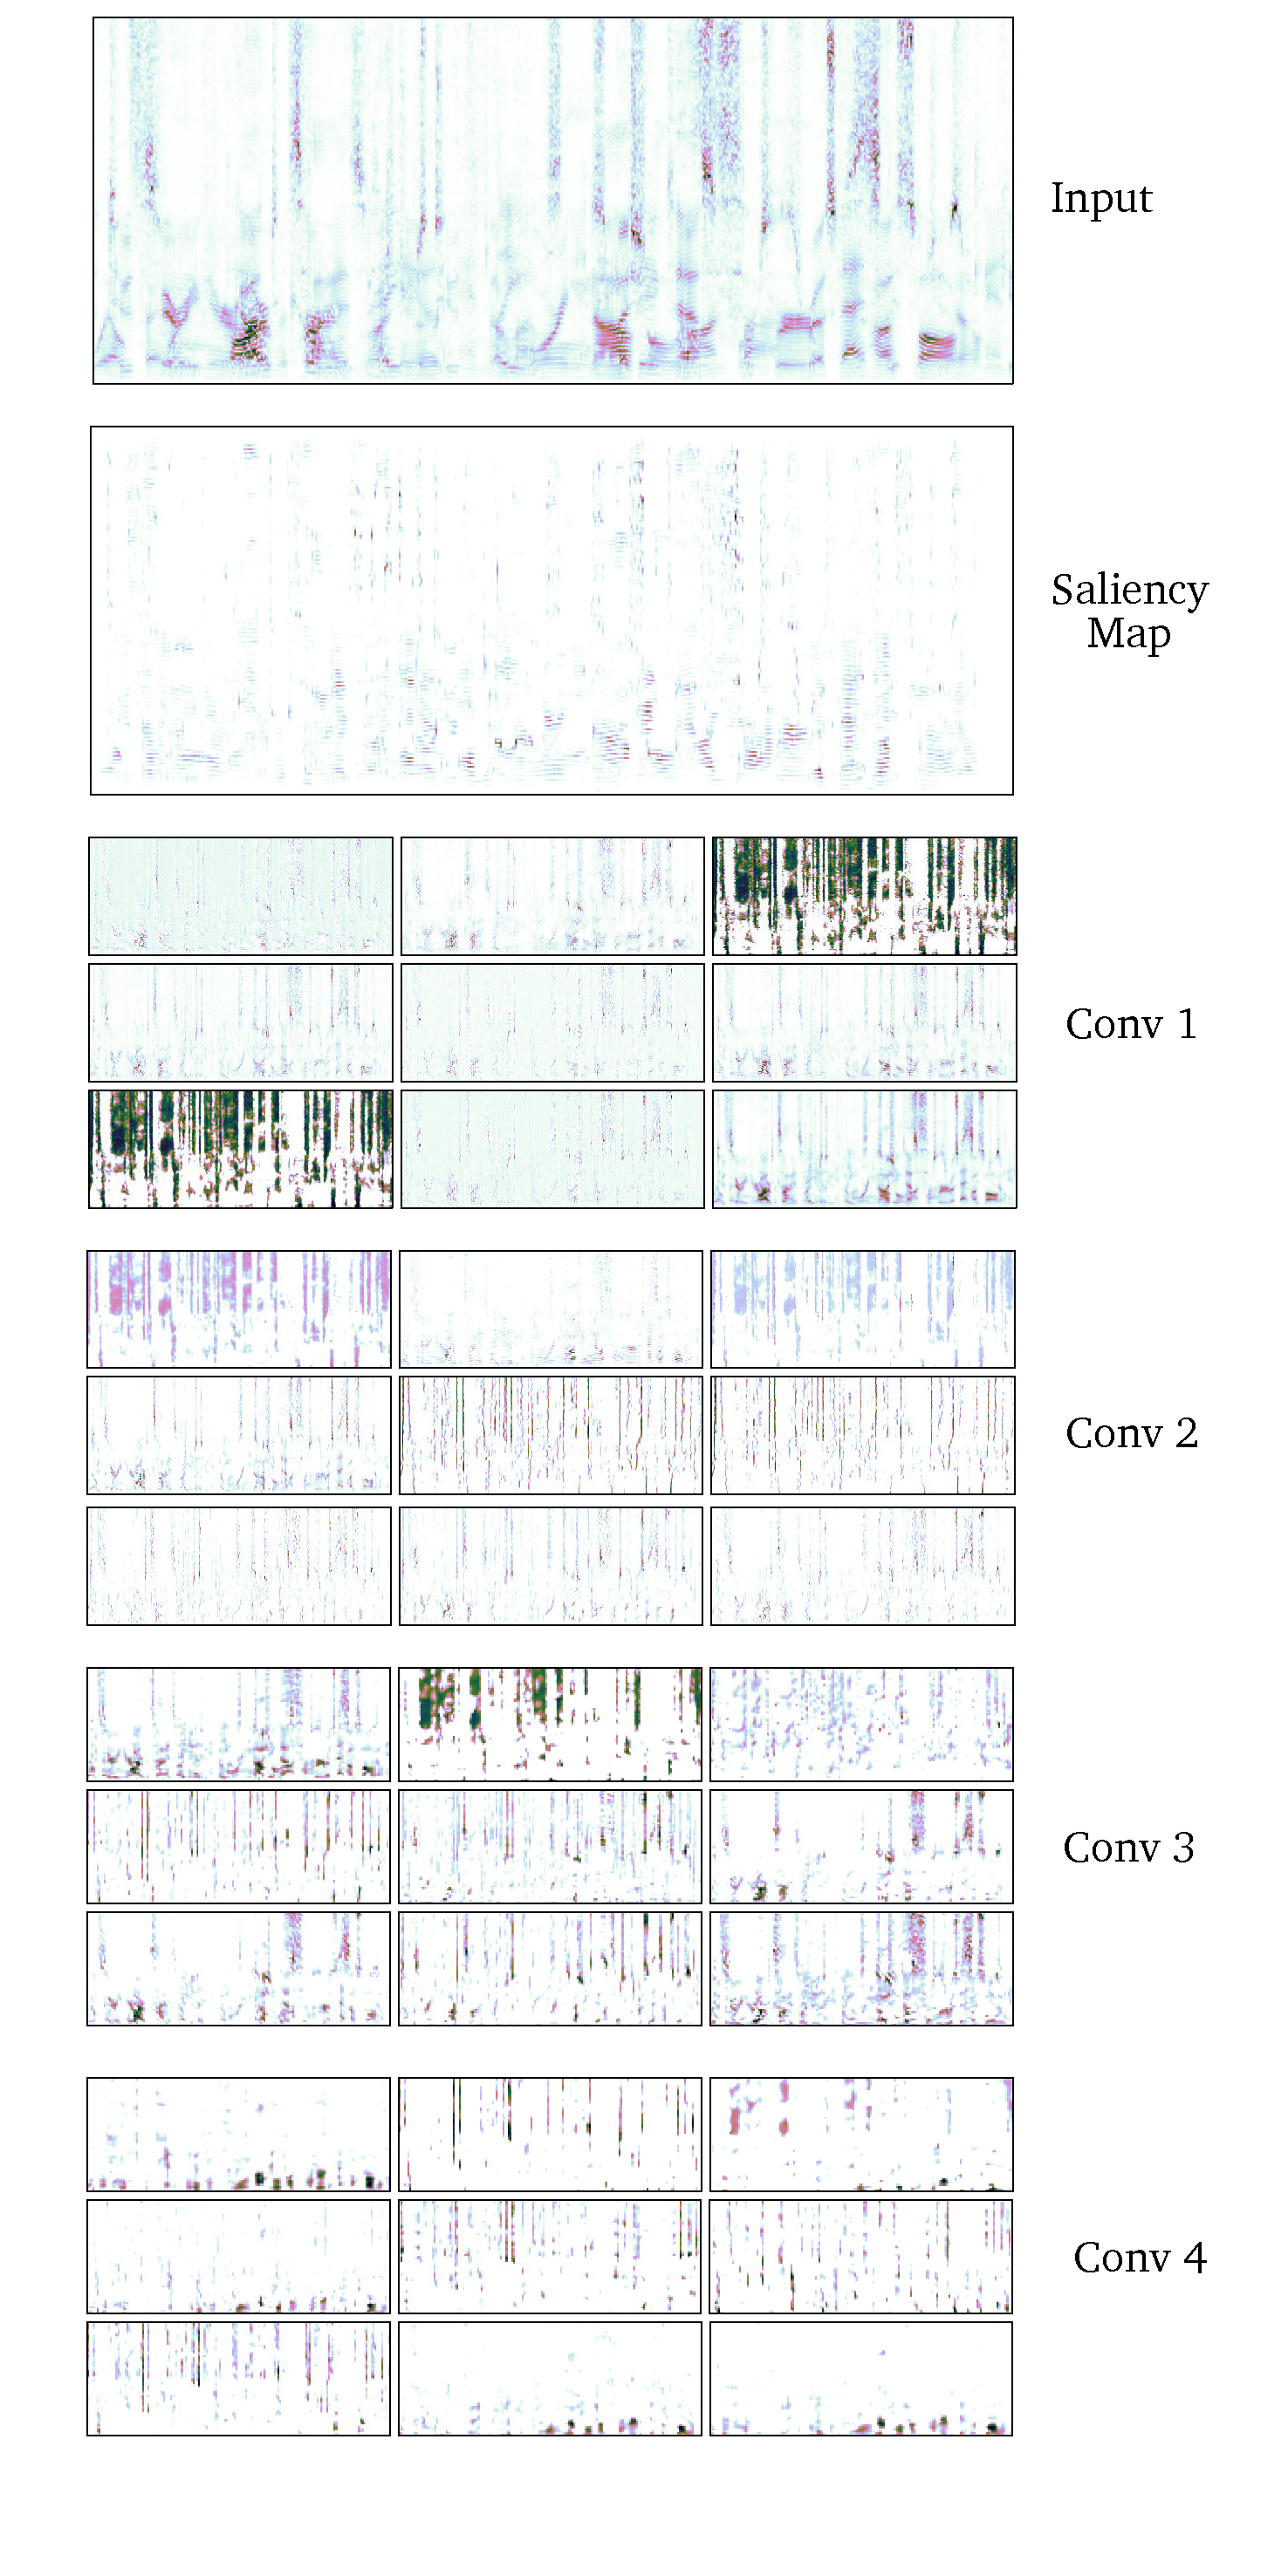
\includegraphics[width=\columnwidth, height=0.7\paperheight, keepaspectratio]{Chapters/dsc/figures/outputs.pdf}
  \caption{Illustration of intermediate outputs from the proposed CRNN for each convolutional layer for a given input with \(k=3\) speakers. Saliency map shows positive saliency of guided backpropagation~\cite{Springenberg14}. For each convolutional layer the nine most relevant filters were selected based on their loss with respect to the input.}%
\label{fig:convoutputs}
\end{figure}
% Select best performing system (CRNN, Classification, STFT) and analyse how it achieves the performance.
In the previous section we showed the effectiveness of the CRNN based model.
Even though \emph{CRNN} achieves very good performance under various conditions, it still remains unclear what strategy the model pursues.
To gain more insight, we conducted a visual analysis based on salience map representations~\cite{Simonyan13}.
% taken from https://github.com/Lasagne/Recipes/blob/master/examples/Saliency%20Maps%20and%20Guided%20Backpropagation.ipynb
In the deep learning context, saliency maps are visualizations that are able to show which specific input elements a neural network used for a particular prediction. This allows an object classifier to be used for object localization or in the case of audio spectrograms, which time frequency bins are most relevant.
The common idea is to compute the gradient of the model's prediction with respect to the input, holding the weights fixed. This determines which input elements need to be changed the least to affect the prediction the most.
\par
In this work we used guided backpropagations, first introduced in~\cite{Springenberg14} and successfully deployed in~\cite{schluter16} to compute a saliency map for singing voice detection.
For a given input spectrogram of a three speaker mixture, we depicted the saliency map in Figure~\ref{fig:convoutputs}.
The saliency map indicates that our proposed model does not rely much on the overlapped parts but instead utilize many of the single speaker time frequency bins.
Also, we can see that both, low frequency harmonic structures as well as many high frequency components such as plosives and fricative phonemes result in increased saliency.
For a more detailed analysis, we also visualized the filtered outputs of the successive convolutional layers.
While we cannot show all filter outputs (e.g. 64, for the first layer), instead for each filter, we compute its loss with respect to the input of the model using gradient update and sort the filters according to their loss.
Figure~\ref{fig:convoutputs} depicts the nine highest loss outputs per convolutional layer.
We can observe that while the first layer shows only low level variations of the input, already the second layer seems to be more abstract and emphasizes phoneme segmentations based on mid and high frequency content.
While filter outputs of layer 3 and 4 also show more low-frequency content such as the harmonic signals, the overall visual impression is that the proposed CRNN focuses on the temporal segmentation of phonemes.
\par
This leads to the hypothesis that the CRNN model learned the aggregated phoneme or syllable activity of all speakers in a fixed, given excerpt.
% \captionof{table}{Binary Logit Regression}\label{Binary Logit Regression}\begin{center}
% \begin{tabular}{lclc}
% \toprule
% \textbf{Dep. Variable:} &      error       & \textbf{  No. Observations:  } &     2000   \\
% \textbf{Model:}         &      Logit       & \textbf{  Df Residuals:      } &     1998   \\
% \textbf{Method:}        &       MLE        & \textbf{  Df Model:          } &        1   \\
% \textbf{Date:}          & Mon, 29 Jan 2018 & \textbf{  Pseudo R-squ.:     } &  0.01108   \\
% \textbf{Time:}          &     16:38:38     & \textbf{  Log-Likelihood:    } &   -1370.9  \\
% \textbf{converged:}     &       True       & \textbf{  LL-Null:           } &   -1386.3  \\
% \textbf{ }              &                  & \textbf{  LLR p-value:       } & 2.980e-08  \\
% \bottomrule
% \end{tabular}
% %\caption{Logit Regression Results}
% \end{center}
If that is the case, it would mean that the speaker count estimate would be affected if the speakers would speak slower or faster in relation to the fixed input window (speaking rate).
We therefore want to see if very slow or very fast speakers significantly increase the error of our proposed CRNN model.
In turn we define a null hypothesis that there is no association between the speaker count error probability and the value of the \emph{speaking rate}.
\par
To verify our hypothesis, we created another experiment based on the \emph{TIMIT} dataset.
It comes with phoneme and word level annotations, from which the speaking rate (defined as syllables per second) can be computed for each input sample~\cite{Jiao16}.
To reduce the influence of the different acoustical environment in TIMIT compared to Libri Speech, we retrained the CRNN classification model on the \emph{TIMIT} training dataset, using the same parameters as described in Section~\ref{sec:training}.
At test time we randomly generated 5 seconds excerpts of \(k=6\) from the TIMIT test subset and predicted the error \(E(k) = \hat{k} - k\) for each CRNN output.
We grouped the estimates into three classes: \(E(k) = 0\) (correct response), \(E(k) > 0\) (overestimation), \(E(k) < 0\) (underestimation).
For \(k=6\) we ended up with two groups of results because overestimation did not take place.
From the remaining two groups \emph{underestimation} and \emph{correct} responses we randomly selected 1000 samples each, resulting in an total sample size of \(n=2000\).
For these samples we computed an average speaking rate of \(3.40\) syllables per second and a standard deviation of \(0.2\).
We chose a Generalized Linear Model (GLM) for the statistical test, as described in~\cite{jaeger08}.
This allows us model the results with a binary logit regression model that turns the mean of E into a binomial distributed probability modeled by log linear values: \(\mbox{logit}(E) \sim \mbox{Intercept} + \beta \cdot{\mbox{Speaking Rate}}\).
\begin{table}[h]
\caption{Results of a binary logit regression test for the dependent variable \emph{correct response} over the independent variable \emph{speaking rate}. The results are based on $n=2000$ randomly drawn results of the CRNN model trained and evaluated on the TIMIT dataset.}%
\label{tab:logit}
\begin{center}
\begin{tabular}{lcccc}
\toprule
                        & \textbf{coef} & \textbf{std err} & \textbf{z} & \textbf{P$>$$|$z$|$} \\
\midrule
\textbf{speaking rate} &      -1.2697   &        0.232     &     -5.477  &         0.000        \\
\textbf{intercept}          &      4.3213  &        0.790     &    5.468  &         0.000  \\
\bottomrule
\end{tabular}
\end{center}
\end{table}
The results of our test are shown in Table~\ref{tab:logit} and indicate the speaking rate has statistically significant influence on the error \(p < 0.05, df=1, \textrm{Pseudo}\ R^2=0.0111\).
To better understand the effect of our predictor, we computed an odds ratio \(\exp(\mbox{speaking rate}) = 0.28\).
This indicates that a decrease in speaking rate of 1 syllable per second will increase the likeliness of an underestimation error by 28 percent.
Even though this is considered as a small effect size, it gives an interesting hint for the strategy taken of our proposed model and also suggests that for improved robustness, training would benefit from a large variety of speaking rates.
Furthermore, it still remains unclear the model would suffer from languages with a speaking rate which is naturally higher or lower than English or Chinese (see~\cite{Osser64}).

\section{Conclusion}%
\label{sec:conclusion}
We introduced the task of estimating the maximum number of concurrent speakers in a simulated ``cocktail-party'' environment using a data-driven approach, discussing how to frame this task in a deep learning context.
Building upon earlier work, we investigated what method is best to output integer source count estimates and also defined suitable cost functions for optimization.
In a comprehensive study we performed experiments to evaluate different network architectures.
Furthermore, we investigated and evaluated other important parameters such as input representations or the input duration.
Our final proposed model uses a convolutional recurrent (CRNN) architecture, based on classification at the network's output.
Compared to several baselines, our proposed model has a significantly lower error rate;
it achieves error rates of less then 0.3 speakers in mean absolute error for classifying zero to ten speakers---a decrease of 28.95\% compared to~\cite{stoeter17}.
In further simulations, we revealed that our model is robust to unseen languages (such as Chinese), as well as varying acoustical conditions (except for reverberation, where the error increased significantly).
However, including reverberate samples in the training reduces the error.
Additionally, we conducted a perceptual experiment showing that these results clearly outperform humans.
Lastly, in an ablation study, we found that the CRNN uses a strategy to segment phonemes/syllables to estimate the count.
Hence, we hypothesize that a speaker count estimate is influenced by the average speaking rates of certain languages.
Finally, to underpin this hypothesis, we showed that the speaking rate has a significant effect on the error of our model.


% \section*{Acknowledgment}
% \addcontentsline{toc}{section}{Acknowledgment}
% The authors gratefully acknowledge the compute resources and support provided by the Erlangen Regional Computing Center (RRZE).
% Special thanks to Antoine Liutkus.

% \nocite{*}
% \clearpage
% \bibliographystyle{IEEEtran}
% \bibliography{references}

% \newpage

% \vspace{-40 mm}
%
% \begin{IEEEbiography}[{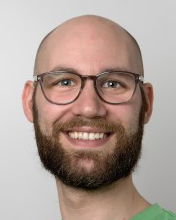
\includegraphics[height=1.25in,keepaspectratio=true]{photos/fabian}}]{Fabian-Robert~St\"{o}ter} received the diploma degree in electrical engineering in 2012 from the Leibniz Universit\"{a}t Hannover and is currently working towards his Ph.D. degree in audio signal processing in the research group of B. Edler at the International Audio Laboratories Erlangen, Germany. His research interests include supervised and unsupervised methods for audio source separation and signal analysis of highly overlapped sources.
% \end{IEEEbiography}
%
% \vspace{-40 mm}
% \begin{IEEEbiography}[{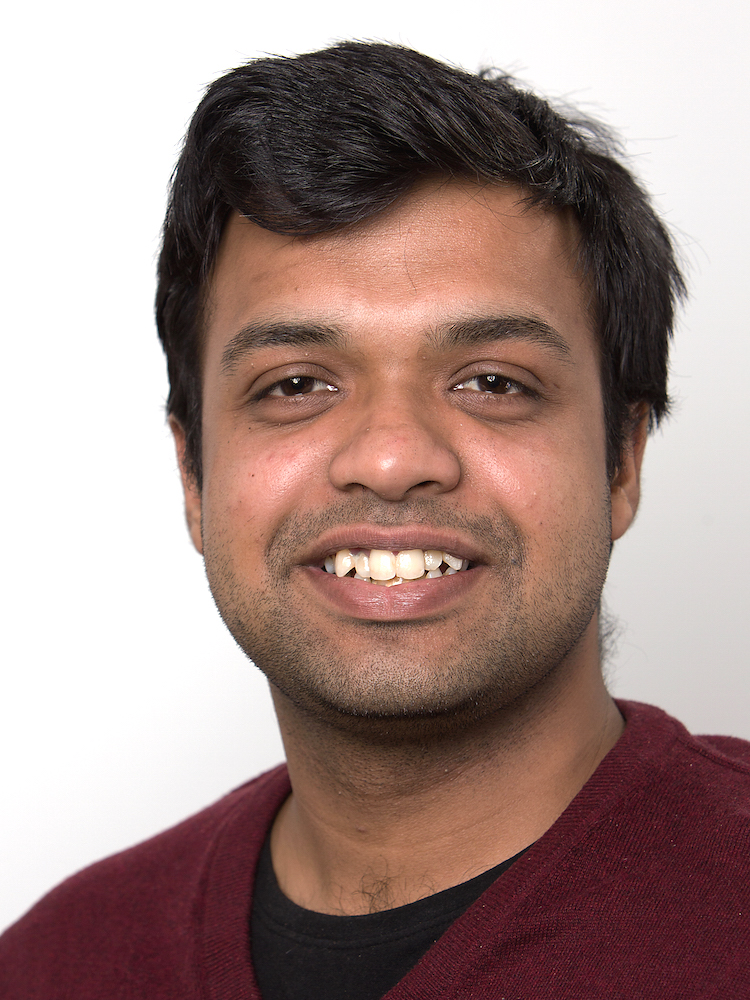
\includegraphics[width=1.25in,height=1.25in,clip,keepaspectratio]{photos/Chakrabarty}}]{Soumitro Chakrabarty} (S'10)
% received his BEng. degree from Manipal University, India in 2010 and his MSc. degree from Ecole Polytechnique Federale de Lausanne, Lausanne, Switzerland in 2013. He is currently pursuing a PhD. at International Audio Laboratories Erlangen, Germany on the topic of robust estimation of spatial information for microphone array processing.
%
% His current research interests include spatial filtering, sound source localization, multi-microphone source extraction and machine learning for array processing.
%
% \end{IEEEbiography}
% \vspace{-40 mm}
% \begin{IEEEbiography}[{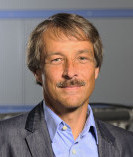
\includegraphics[height=1.25in,keepaspectratio=true]{photos/edler}}]{Bernd Edler} Lorem ipsum dolor sit amet, consectetur adipisicing elit, sed do eiusmod tempor incididunt ut labore et dolore magna aliqua. Ut enim ad minim veniam, quis nostrud exercitation ullamco laboris nisi ut aliquip ex ea commodo consequat. Duis aute irure dolor in reprehenderit in voluptate velit esse cillum dolore eu fugiat nulla pariatur. Excepteur sint occaecat cupidatat non proident, sunt in culpa qui officia deserunt mollit anim id est laborum.
% \end{IEEEbiography}
% \vspace{-40 mm}
% \begin{IEEEbiography}[{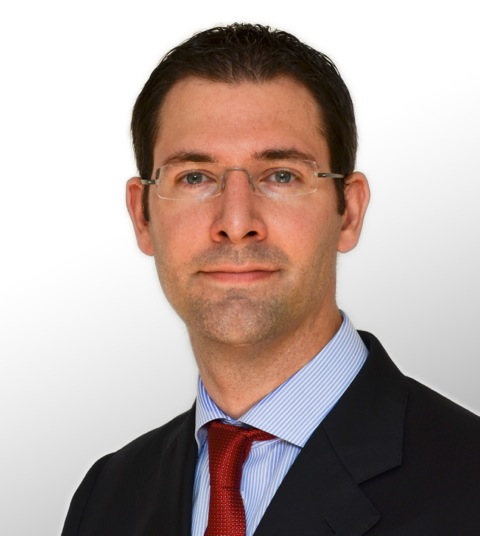
\includegraphics[width=1.25in,height=1.25in,clip,keepaspectratio]{photos/Habets}}]{Emanu\"{e}l A.P. Habets} (S'02-M'07-SM'11)
% is an Associate Professor at the International Audio Laboratories Erlangen (a joint institution of the Friedrich-Alexander-Universit\"{a}t Erlangen-N\"{u}rnberg and Fraunhofer IIS), and Head of the Spatial Audio Research Group at Fraunhofer IIS, Germany. He received the B.Sc. degree in electrical engineering from the Hogeschool Limburg, The Netherlands, in 1999, and the M.Sc. and Ph.D. degrees in electrical engineering from the Technische Universiteit Eindhoven, The Netherlands, in 2002 and 2007, respectively.
%
% From 2007 until 2009, he was a Postdoctoral Fellow at the Technion - Israel Institute of Technology and at the Bar-Ilan University, Israel. From 2009 until 2010, he was a Research Fellow in the Communication and Signal Processing Group at Imperial College London, U.K.
%
% His research activities center around audio and acoustic signal processing, and include spatial audio signal processing, spatial sound recording and reproduction, speech enhancement (dereverberation, noise reduction, echo reduction), and sound localization and tracking.
%
% Dr. Habets was a member of the organization committee of the 2005 International Workshop on Acoustic Echo and Noise Control (IWAENC) in Eindhoven, The Netherlands, a general co-chair of the 2013 International Workshop on Applications of Signal Processing to Audio and Acoustics (WASPAA) in New Paltz, New York, and general co-chair of the 2014 International Conference on Spatial Audio (ICSA) in Erlangen, Germany. He was a member of the IEEE Signal Processing Society Standing Committee on Industry Digital Signal Processing Technology (2013-2015), a Guest Editor for the IEEE Journal of Selected Topics in Signal Processing and the EURASIP Journal on Advances in Signal Processing, and an Associate Editor of the IEEE Signal Processing Letters (2013-2017). He is the recipient, with S. Gannot and I. Cohen, of the 2014 IEEE Signal Processing Letters Best Paper Award. Currently, he is a member of the IEEE Signal Processing Society Technical Committee on Audio and Acoustic Signal Processing, vice-chair of the EURASIP Special Area Team on Acoustic, Sound and Music Signal Processing, and Editor in Chief of the EURASIP Journal on Audio, Speech, and Music Processing.
% \end{IEEEbiography}
% \enlargethispage{-20.5cm}
% \end{document}




%\addtocontents{toc}{\protect\clearpage} % <--- just debug stuff, ignore
% %************************************************
\chapter{Math Test Chapter}\label{ch:mathtest} % $\mathbb{ZNR}$
%************************************************
Ei choro aeterno antiopam mea, labitur bonorum pri no. His no decore
nemore graecis. In eos meis nominavi, liber soluta vim cu. Sea commune
suavitate interpretaris eu, vix eu libris efficiantur.

\section{Some Formulas}
Due to the statistical nature of ionisation energy loss, large
fluctuations can occur in the amount of energy deposited by a particle
traversing an absorber element\footnote{Examples taken from Walter
Schmidt's great gallery: \\
\url{http://home.vrweb.de/~was/mathfonts.html}}.  Continuous processes
such as multiple
scattering and energy loss play a relevant role in the longitudinal
and lateral development of electromagnetic and hadronic
showers, and in the case of sampling calorimeters the
measured resolution can be significantly affected by such fluctuations
in their active layers.  The description of ionisation fluctuations is
characterised by the significance parameter $\kappa$, which is
proportional to the ratio of mean energy loss to the maximum allowed
energy transfer in a single collision with an atomic electron:
\graffito{You might get unexpected results using math in chapter or
section heads. Consider the \texttt{pdfspacing} option.}
\begin{equation}
\kappa =\frac{\xi}{E_{\textrm{max}}} %\mathbb{ZNR}
\end{equation}
$E_{\textrm{max}}$ is the maximum transferable energy in a single
collision with an atomic electron.
\[
E_{\textrm{max}} =\frac{2 m_{\textrm{e}} \beta^2\gamma^2 }{1 +
2\gamma m_{\textrm{e}}/m_{\textrm{x}} + \left ( m_{\textrm{e}}
/m_{\textrm{x}}\right)^2}\ ,
\]
where $\gamma = E/m_{\textrm{x}}$, $E$ is energy and
$m_{\textrm{x}}$ the mass of the incident particle,
$\beta^2 = 1 - 1/\gamma^2$ and $m_{\textrm{e}}$ is the electron mass.
$\xi$ comes from the Rutherford scattering cross section
and is defined as:
\begin{eqnarray*} \xi  = \frac{2\pi z^2 e^4 N_{\textrm{Av}} Z \rho
\delta x}{m_{\textrm{e}} \beta^2 c^2 A} =  153.4 \frac{z^2}{\beta^2}
\frac{Z}{A}
  \rho \delta x \quad\textrm{keV},
\end{eqnarray*}
where

\begin{tabular}{ll}
$z$          & charge of the incident particle \\
$N_{\textrm{Av}}$     & Avogadro's number \\
$Z$          & atomic number of the material \\
$A$          & atomic weight of the material \\
$\rho$       & density \\
$ \delta x$  & thickness of the material \\
\end{tabular}

$\kappa$ measures the contribution of the collisions with energy
transfer close to $E_{\textrm{max}}$.  For a given absorber, $\kappa$
tends
towards large values if $\delta x$ is large and/or if $\beta$ is
small.  Likewise, $\kappa$ tends towards zero if $\delta x $ is small
and/or if $\beta$ approaches $1$.

The value of $\kappa$ distinguishes two regimes which occur in the
description of ionisation fluctuations:

\begin{enumerate}
\item A large number of collisions involving the loss of all or most
    of the incident particle energy during the traversal of an absorber.

    As the total energy transfer is composed of a multitude of small
    energy losses, we can apply the central limit theorem and describe
    the fluctuations by a Gaussian distribution.  This case is
    applicable to non-relativistic particles and is described by the
    inequality $\kappa > 10 $ (\ie, when the mean energy loss in the
    absorber is greater than the maximum energy transfer in a single
    collision).

\item Particles traversing thin counters and incident electrons under
    any conditions.

    The relevant inequalities and distributions are $ 0.01 < \kappa < 10
    $,
    Vavilov distribution, and $\kappa < 0.01 $, Landau distribution.
\end{enumerate}


\section{Various Mathematical Examples}
If $n > 2$, the identity
\[
    t[u_1,\dots,u_n] = t\bigl[t[u_1,\dots,u_{n_1}], t[u_2,\dots,u_n]
    \bigr]
\]
defines $t[u_1,\dots,u_n]$ recursively, and it can be shown that the
alternative definition
\[
    t[u_1,\dots,u_n] = t\bigl[t[u_1,u_2],\dots,t[u_{n-1},u_n]\bigr]
\]
gives the same result.

%*****************************************
%*****************************************
%*****************************************
%*****************************************
%*****************************************

%\include{multiToC} % <--- just debug stuff, ignore for your documents
% ********************************************************************
% Backmatter
%*******************************************************
\appendix
%\renewcommand{\thechapter}{\alph{chapter}}
\cleardoublepage
\part{Appendix}
% %********************************************************************
% Appendix
%*******************************************************
% If problems with the headers: get headings in appendix etc. right
%\markboth{\spacedlowsmallcaps{Appendix}}{\spacedlowsmallcaps{Appendix}}
\chapter{Appendix Test}
Lorem ipsum at nusquam appellantur his, ut eos erant homero
concludaturque. Albucius appellantur deterruisset id eam, vivendum
partiendo dissentiet ei ius. Vis melius facilisis ea, sea id convenire
referrentur, takimata adolescens ex duo. Ei harum argumentum per. Eam
vidit exerci appetere ad, ut vel zzril intellegam interpretaris.

Errem omnium ea per, pro congue populo ornatus cu, ex qui dicant
nemore melius. No pri diam iriure euismod. Graecis eleifend
appellantur quo id. Id corpora inimicus nam, facer nonummy ne pro,
kasd repudiandae ei mei. Mea menandri mediocrem dissentiet cu, ex
nominati imperdiet nec, sea odio duis vocent ei. Tempor everti
appareat cu ius, ridens audiam an qui, aliquid admodum conceptam ne
qui. Vis ea melius nostrum, mel alienum euripidis eu.

\section{Appendix Section Test}
Ei choro aeterno antiopam mea, labitur bonorum pri no. His no decore
nemore graecis. In eos meis nominavi, liber soluta vim cu. Sea commune
suavitate interpretaris eu, vix eu libris efficiantur.

\autoref{tab:moreexample}

\graffito{More dummy text.}
Nulla fastidii ea ius, exerci suscipit instructior te nam, in ullum
postulant quo. Congue quaestio philosophia his at, sea odio autem
vulputate ex. Cu usu mucius iisque voluptua. Sit maiorum propriae at,
ea cum primis intellegat. Hinc cotidieque reprehendunt eu nec. Autem
timeam deleniti usu id, in nec nibh altera.

\section{Another Appendix Section Test}
Equidem detraxit cu nam, vix eu delenit periculis. Eos ut vero
constituto, no vidit propriae complectitur sea. Diceret nonummy in
has, no qui eligendi recteque consetetur. Mel eu dictas suscipiantur,
et sed placerat oporteat. At ipsum electram mei, ad aeque atomorum
mea.

\begin{table}
    \myfloatalign
  \begin{tabularx}{\textwidth}{Xll} \toprule
    \tableheadline{labitur bonorum pri no} & \tableheadline{que vista}
    & \tableheadline{human} \\ \midrule
    fastidii ea ius & germano &  demonstratea \\
    suscipit instructior & titulo & personas \\
    %postulant quo & westeuropee & sanctificatec \\
    \midrule
    quaestio philosophia & facto & demonstrated \\
    %autem vulputate ex & parola & romanic \\
    %usu mucius iisque & studio & sanctificatef \\
    \bottomrule
  \end{tabularx}
  \caption[Autem usu id]{Autem usu id.}
  \label{tab:moreexample}
\end{table}

Ei solet nemore consectetuer nam. Ad eam porro impetus, te choro omnes
evertitur mel. Molestie conclusionemque vel at, no qui omittam
expetenda efficiendi. Eu quo nobis offendit, verterem scriptorem ne
vix.

  
\begin{lstlisting}[float,caption=A floating example]
for i:=maxint to 0 do
begin
{ do nothing }
end;
\end{lstlisting}
%********************************************************************
% Other Stuff in the Back
%*******************************************************
\cleardoublepage%********************************************************************
% Bibliography
%*******************************************************
% work-around to have small caps also here in the headline
% https://tex.stackexchange.com/questions/188126/wrong-header-in-bibliography-classicthesis
% Thanks to Enrico Gregorio
\defbibheading{bibintoc}[\bibname]{%
  \phantomsection
  \manualmark
  \markboth{\spacedlowsmallcaps{#1}}{\spacedlowsmallcaps{#1}}%
  \addtocontents{toc}{\protect\vspace{\beforebibskip}}%
  \addcontentsline{toc}{chapter}{\tocEntry{#1}}%
  \chapter*{#1}%
}
\printbibliography[heading=bibintoc]

% Old version, will be removed later
% work-around to have small caps also here in the headline
%\manualmark
%\markboth{\spacedlowsmallcaps{\bibname}}{\spacedlowsmallcaps{\bibname}} % work-around to have small caps also
%\phantomsection
%\refstepcounter{dummy}
%\addtocontents{toc}{\protect\vspace{\beforebibskip}} % to have the bib a bit from the rest in the toc
%\addcontentsline{toc}{chapter}{\tocEntry{\bibname}}
%\label{app:bibliography}
%\printbibliography

\cleardoublepage%*******************************************************
% Declaration
%*******************************************************
\refstepcounter{dummy}
\pdfbookmark[0]{Declaration}{declaration}
\chapter*{Declaration}
\thispagestyle{empty}
Put your declaration here.
\bigskip

\noindent\textit{\myLocation, \myTime}

\smallskip

\begin{flushright}
    \begin{tabular}{m{5cm}}
        \\ \hline
        \centering\myName \\
    \end{tabular}
\end{flushright}

\cleardoublepage\pagestyle{empty}

\hfill

\vfill


\pdfbookmark[0]{Colophon}{colophon}
\section*{Colophon}
This document was typeset using the typographical look-and-feel \texttt{classicthesis} developed by Andr\'e Miede. 
The style was inspired by Robert Bringhurst's seminal book on typography ``\emph{The Elements of Typographic Style}''. 
\texttt{classicthesis} is available for both \LaTeX\ and \mLyX: 
\begin{center}
\url{https://bitbucket.org/amiede/classicthesis/}
\end{center}
Happy users of \texttt{classicthesis} usually send a real postcard to the author, a collection of postcards received so far is featured here: 
\begin{center}
\url{http://postcards.miede.de/}
\end{center}
 
\bigskip

\noindent\finalVersionString

%Hermann Zapf's \emph{Palatino} and \emph{Euler} type faces (Type~1 PostScript fonts \emph{URW
%Palladio L} and \emph{FPL}) are used. The ``typewriter'' text is typeset in \emph{Bera Mono}, 
%originally developed by Bitstream, Inc. as ``Bitstream Vera''. (Type~1 PostScript fonts were made 
%available by Malte Rosenau and
%Ulrich Dirr.)

%\paragraph{note:} The custom size of the textblock was calculated
%using the directions given by Mr. Bringhurst (pages 26--29 and
%175/176). 10~pt Palatino needs  133.21~pt for the string
%``abcdefghijklmnopqrstuvwxyz''. This yields a good line length between
%24--26~pc (288--312~pt). Using a ``\emph{double square textblock}''
%with a 1:2 ratio this results in a textblock of 312:624~pt (which
%includes the headline in this design). A good alternative would be the
%``\emph{golden section textblock}'' with a ratio of 1:1.62, here
%312:505.44~pt. For comparison, \texttt{DIV9} of the \texttt{typearea}
%package results in a line length of 389~pt (32.4~pc), which is by far
%too long. However, this information will only be of interest for
%hardcore pseudo-typographers like me.%
%
%To make your own calculations, use the following commands and look up
%the corresponding lengths in the book:
%\begin{verbatim}
%    \settowidth{\abcd}{abcdefghijklmnopqrstuvwxyz}
%    \the\abcd\ % prints the value of the length
%\end{verbatim}
%Please see the file \texttt{classicthesis.sty} for some precalculated 
%values for Palatino and Minion.
%
%    \settowidth{\abcd}{abcdefghijklmnopqrstuvwxyz}
%    \the\abcd\ % prints the value of the length





% ********************************************************************
% Game Over: Restore, Restart, or Quit?
%*******************************************************
\end{document}
% ********************************************************************
